% This is the Reed College LaTeX thesis template. Most of the work
% for the document class was done by Sam Noble (SN), as well as this
% template. Later comments etc. by Ben Salzberg (BTS). Additional
% restructuring and APA support by Jess Youngberg (JY).
% Your comments and suggestions are more than welcome; please email
% them to cus@reed.edu
%
% See https://www.reed.edu/cis/help/LaTeX/index.html for help. There are a
% great bunch of help pages there, with notes on
% getting started, bibtex, etc. Go there and read it if you're not
% already familiar with LaTeX.
%
% Any line that starts with a percent symbol is a comment.
% They won't show up in the document, and are useful for notes
% to yourself and explaining commands.
% Commenting also removes a line from the document;
% very handy for troubleshooting problems. -BTS

% As far as I know, this follows the requirements laid out in
% the 2002-2003 Senior Handbook. Ask a librarian to check the
% document before binding. -SN

%%
%% Preamble
%%
% \documentclass{<something>} must begin each LaTeX document
\pdfobjcompresslevel 0 % voir https://facile.cines.fr#latex
\documentclass[12pt,a4paper]{reedthesis}
% Packages are extensions to the basic LaTeX functions. Whatever you
% want to typeset, there is probably a package out there for it.
% Chemistry (chemtex), screenplays, you name it.
% Check out CTAN to see: https://www.ctan.org/
%%
\usepackage{graphicx,latexsym}
\usepackage{amsmath,amssymb,amsthm}
\usepackage{amsfonts}
\usepackage{bbm}
\usepackage{longtable,booktabs,setspace}
\usepackage[hyphens]{url}
% Added by CII
\usepackage{lmodern}
\usepackage{float}
\floatplacement{figure}{H}
% End of CII addition
\usepackage{rotating}
\usepackage[french,english]{babel}

\usepackage[utf8]{inputenc}
\usepackage[scaled]{berasans}
\usepackage[T1]{fontenc}
\usepackage{fancyhdr}
\usepackage{xcolor}
\definecolor{Prune}{RGB}{99,0,60}
\usepackage{mdframed}
\usepackage{multirow} %% Pour mettre un texte sur plusieurs rangées
\usepackage{multicol} %% Pour mettre un texte sur plusieurs colonnes
\usepackage{scrextend} %Forcer la 4eme de couverture en page pair
\usepackage{tikz}
\usepackage[absolute]{textpos}
\usepackage{colortbl}
\usepackage{array}
%\RequirePackage{geometry}% That nicely create a one-page template
%\geometry{textheight=100ex,textwidth=40em,top=30pt,headheight=30pt,headsep=30pt,inner=80pt}
\usepackage{geometry}
\usepackage{hyperref}

% Next line commented out by CII
%%% \usepackage{natbib}
% Comment out the natbib line above and uncomment the following two lines to use the new
% biblatex-chicago style, for Chicago A. Also make some changes at the end where the
% bibliography is included.
%\usepackage{biblatex-chicago}
%\bibliography{thesis}


% Added by CII (Thanks, Hadley!)
% Use ref for internal links
\renewcommand{\hyperref}[2][???]{\autoref{#1}}
\def\chapterautorefname{Chapter}
\def\sectionautorefname{Section}
\def\subsectionautorefname{Subsection}
% End of CII addition

% Added by CII
\usepackage{caption}
\captionsetup{width=5in}
% End of CII addition

% \usepackage{times} % other fonts are available like times, bookman, charter, palatino

% Syntax highlighting #22
  \usepackage{color}
  \usepackage{fancyvrb}
  \newcommand{\VerbBar}{|}
  \newcommand{\VERB}{\Verb[commandchars=\\\{\}]}
  \DefineVerbatimEnvironment{Highlighting}{Verbatim}{commandchars=\\\{\}}
  % Add ',fontsize=\small' for more characters per line
  \usepackage{framed}
  \definecolor{shadecolor}{RGB}{248,248,248}
  \newenvironment{Shaded}{\begin{snugshade}}{\end{snugshade}}
  \newcommand{\AlertTok}[1]{\textcolor[rgb]{0.94,0.16,0.16}{#1}}
  \newcommand{\AnnotationTok}[1]{\textcolor[rgb]{0.56,0.35,0.01}{\textbf{\textit{#1}}}}
  \newcommand{\AttributeTok}[1]{\textcolor[rgb]{0.77,0.63,0.00}{#1}}
  \newcommand{\BaseNTok}[1]{\textcolor[rgb]{0.00,0.00,0.81}{#1}}
  \newcommand{\BuiltInTok}[1]{#1}
  \newcommand{\CharTok}[1]{\textcolor[rgb]{0.31,0.60,0.02}{#1}}
  \newcommand{\CommentTok}[1]{\textcolor[rgb]{0.56,0.35,0.01}{\textit{#1}}}
  \newcommand{\CommentVarTok}[1]{\textcolor[rgb]{0.56,0.35,0.01}{\textbf{\textit{#1}}}}
  \newcommand{\ConstantTok}[1]{\textcolor[rgb]{0.00,0.00,0.00}{#1}}
  \newcommand{\ControlFlowTok}[1]{\textcolor[rgb]{0.13,0.29,0.53}{\textbf{#1}}}
  \newcommand{\DataTypeTok}[1]{\textcolor[rgb]{0.13,0.29,0.53}{#1}}
  \newcommand{\DecValTok}[1]{\textcolor[rgb]{0.00,0.00,0.81}{#1}}
  \newcommand{\DocumentationTok}[1]{\textcolor[rgb]{0.56,0.35,0.01}{\textbf{\textit{#1}}}}
  \newcommand{\ErrorTok}[1]{\textcolor[rgb]{0.64,0.00,0.00}{\textbf{#1}}}
  \newcommand{\ExtensionTok}[1]{#1}
  \newcommand{\FloatTok}[1]{\textcolor[rgb]{0.00,0.00,0.81}{#1}}
  \newcommand{\FunctionTok}[1]{\textcolor[rgb]{0.00,0.00,0.00}{#1}}
  \newcommand{\ImportTok}[1]{#1}
  \newcommand{\InformationTok}[1]{\textcolor[rgb]{0.56,0.35,0.01}{\textbf{\textit{#1}}}}
  \newcommand{\KeywordTok}[1]{\textcolor[rgb]{0.13,0.29,0.53}{\textbf{#1}}}
  \newcommand{\NormalTok}[1]{#1}
  \newcommand{\OperatorTok}[1]{\textcolor[rgb]{0.81,0.36,0.00}{\textbf{#1}}}
  \newcommand{\OtherTok}[1]{\textcolor[rgb]{0.56,0.35,0.01}{#1}}
  \newcommand{\PreprocessorTok}[1]{\textcolor[rgb]{0.56,0.35,0.01}{\textit{#1}}}
  \newcommand{\RegionMarkerTok}[1]{#1}
  \newcommand{\SpecialCharTok}[1]{\textcolor[rgb]{0.00,0.00,0.00}{#1}}
  \newcommand{\SpecialStringTok}[1]{\textcolor[rgb]{0.31,0.60,0.02}{#1}}
  \newcommand{\StringTok}[1]{\textcolor[rgb]{0.31,0.60,0.02}{#1}}
  \newcommand{\VariableTok}[1]{\textcolor[rgb]{0.00,0.00,0.00}{#1}}
  \newcommand{\VerbatimStringTok}[1]{\textcolor[rgb]{0.31,0.60,0.02}{#1}}
  \newcommand{\WarningTok}[1]{\textcolor[rgb]{0.56,0.35,0.01}{\textbf{\textit{#1}}}}


% Added by CII
%%% Copied from knitr
%% maxwidth is the original width if it's less than linewidth
%% otherwise use linewidth (to make sure the graphics do not exceed the margin)
\makeatletter
\def\maxwidth{ %
  \ifdim\Gin@nat@width>\linewidth
    \linewidth
  \else
    \Gin@nat@width
  \fi
}
\makeatother

%Added by @MyKo101, code provided by @GerbrichFerdinands

\renewcommand{\contentsname}{Table of Contents}
% End of CII addition

\setlength{\parskip}{0pt}

% Added by CII

\providecommand{\tightlist}{%
  \setlength{\itemsep}{0pt}\setlength{\parskip}{0pt}}

	\usepackage{color}
\usepackage{mathrsfs}
% Sets
\newcommand \NN {\mathbb{N}}
\newcommand \ZZ {\mathbb{Z}}
\newcommand \QQ {\mathbb{Q}}
\newcommand \RR {\mathbb{R}}
\newcommand \shiftset {\mathcal{D}}
% dx
\newcommand \dx [2] [] {\mathrm{d}^{#1}\mspace{-1mu}\mathord{#2}}
% Indicator
\newcommand \indic {\mathbbm{1}}
% Probability Operators
\DeclareMathOperator*{\prob}{\mathbb{P}}
\DeclareMathOperator*{\esp}{\mathbb{E}}
\DeclareMathOperator*{\var}{\mathbb{V}\text{ar}}
\DeclareMathOperator*{\cov}{\mathbb{C}\text{ov}}
\newcommand \PP [1]{\prob\left({#1}\right)}
\newcommand \EE [1]{\esp\left[{#1}\right]}
\newcommand \VV [1]{\var\left[{#1}\right]}
\newcommand \CC [1]{\cov\left[{#1}\right]}
% Law
\newcommand \unif [1] {\mathcal{U}\left({#1}\right)}
\newcommand \normal [2] {\mathcal{N}\left({#1},{#2}\right)}
\newcommand \ou [1]{{#1}_{\text{ou}}}
\newcommand \oui [2]{{#1}_{\text{ou},#2}}
% pv qv zs ts
\newcommand \pv {\mathfrak{p}}
\newcommand \qv {\mathfrak{q}}
\newcommand \zs {\mathfrak{z}}
\newcommand \ts {\mathfrak{t}}
\newcommand \sign {\mathfrak{s}}
% Usual vectors
\newcommand \shifts {\delta}
\newcommand \optim {\beta}
\newcommand \param {\theta}
% Operators
\DeclareMathOperator*{\argmin}{argmin}
% Matrix
\DeclareMathOperator*{\diag}{Diag}
\DeclareMathOperator*{\rang}{rang}
% Tree
\DeclareMathOperator*{\pa}{pa}
\DeclareMathOperator*{\mrca}{mrca}
\DeclareMathOperator*{\desc}{desc}
% Color
\newcommand \warning [1] {\textcolor{red}{#1}}
% End of CII addition
%%
%% End Preamble
%%
%

\usepackage{amsthm}
\newtheorem{theorem}{Théoreme}[chapter]
\newtheorem{lemma}{Lemme}[chapter]
\newtheorem{corollary}{Corollaire}[chapter]
\newtheorem{proposition}{Proposition}[chapter]
\newtheorem{conjecture}{Conjecture}[chapter]
\theoremstyle{definition}
\newtheorem{definition}{Définition}[chapter]
\theoremstyle{definition}
\newtheorem{example}{Exemple}[chapter]
\theoremstyle{definition}
\newtheorem{exercise}{Exercice}[chapter]
\theoremstyle{remark}
\newtheorem*{remark}{Remarque}
\newtheorem*{solution}{Solution}
\begin{document}
\selectlanguage{french}
\begin{titlepage}

%\thispagestyle{empty}

\newgeometry{left=7.5cm,bottom=2cm, top=1cm, right=1cm}
\tikz[remember picture,overlay] \node[opacity=1,inner sep=0pt] at (-28mm,-135mm){
\includegraphics{logos/bandeau.pdf}};

% fonte sans empattement pour la page de titre
\fontfamily{fvs}\fontseries{m}\selectfont

%*****************************************************
%******** NUMÉRO D'ORDRE DE LA THÈSE À COMPLÉTER  ****
%******** après le premier dépôt légal /          ****
%******** French legal PhD number to be completed ****
%******** after the first legal deposit           ****
%*****************************************************

\color{white}
\begin{picture}(0,0)
\put(-150,-735){\rotatebox{90}{NNT~: 2020UPASM016}}
\end{picture}
%*************************************************************
%**  LOGO  ÉTABLISSEMENT PARTENAIRE SI COTUTELLE :          **
%**  CHANGER L'IMAGE logoCotutelle.png; SINON COMMENTER  /  **
%**  Logo of partner establishment if cotutelle agreement : **
%**  change image logoCotutelle.png; otherwise add % signs  **
%*************************************************************
\vspace{10mm}

%*****************************************************
%**************** TITRE / TITLE **********************
%*****************************************************
\flushright
\vspace{15mm} % largeur à régler éventuellement / width to adjust if necessary
\color{Prune}
\fontfamily{fvs}\fontseries{m}\fontsize{22}{26}\selectfont
  Prise en compte de l'organisation hiérarchique des espèces pour la découverte de signatures métagénomiques multi-échelles


%*****************************************************

%\fontfamily{fvs}\fontseries{m}\fontsize{8}{12}\selectfont
\normalsize
\vspace{15mm}

\color{black}
\textbf{Thèse de doctorat de l'Université Paris-Saclay}

\vspace{10mm}

\hspace*{-0.7cm}École Doctorale de Mathématique Hadamard (EDMH) n°574\\
\small Spécialité de doctorat~: Mathématiques appliquées\\
\footnotesize Unité de recherche~: Université Paris-Saclay, CNRS, Univ Évry, Laboratoire de Mathématiques et Modélisation d'Évry, 91037, Évry-Courcouronnes, France\\
\footnotesize Référent~: Université d'Évry

\vspace{10mm}

\textbf{Thèse présentée et soutenue à Paris, le 9 décembre 2020, par}
\bigskip
\Large {\color{Prune} \textbf{Antoine BICHAT}}


\vspace{15mm}


\flushleft \normalsize \textbf{Composition du jury~:}
\bigskip


\scriptsize
\arrayrulecolor{Prune}
\begin{tabular}{|p{8cm}l}
\textbf{Nathalie VIALANEIX} &  Présidente\\
Directrice de recherche -- INRAE Toulouse & \\
\textbf{Étienne ROQUAIN} &  Rapporteur et examinateur\\
Maître de conférences, HdR -- Sorbonne Université & \\
\textbf{Joseph SALMON} &  Rapporteur et examinateur\\
Professeur des universités -- Université de Montpellier & \\
\textbf{Julie AUBERT} &  Examinatrice\\
Ingénieure de recherche -- INRAE Paris & \\
\textbf{Agathe GUILLOUX} &  Examinatrice\\
Professeure des universités -- Université d'Évry & \\
\textbf{Matthieu PICHAUD} &  Examinateur\\
Danone & \\
\end{tabular}
\begin{tabular}{p{8cm}l}
& \\
\textbf{Christophe AMBROISE} &  Directeur\\
Professeur des universités -- Université d'Évry & \\
\textbf{Mahendra MARIADASSOU} &  Co-encadrant\\
Chargé de recherche -- INRAE Jouy-en-Josas & \\
\textbf{Jonathan PLASSAIS} &  Invité\\
Stat-Alliance & \\
\end{tabular}
\end{titlepage}
\frontmatter % this stuff will be roman-numbered
\pagestyle{empty} % this removes page numbers from the frontmatter
  \begin{acknowledgements}
    Mes premiers remerciements vont naturellement à mes directeurs de thèse, Christophe Ambroise et Mahendra Mariadassou. Merci à vous de m'avoir guidé, soutenu, et épaulé pendant ces trois années sous vos ailes, avec votre culture scientifique, votre patience et votre dévouement. Merci à Jonathan Plassais de m'avoir accompagné cette première année de thèse, et à Francesco Strozzi d'avoir pris le relais. J'ai énormément appris avec vous !
    
    \vspace{5mm}
    
    Merci à Étienne Roquain et Joseph Salmon d'avoir accepté de rapporter ma thèse, ainsi qu'à Julie Aubert, Agathe Guilloux, Matthieu Pichaud et Nathalie Vialaneix de m'avoir fait l'honneur d'être dans mon jury, vos remarques ont contribué à améliorer mon manuscrit.
    
    \vspace{5mm}
    
    Je tiens à remercier toute la société Enterome, qui m'a accueilli pendant ces trois ans. Merci à Jonathan et Alessandra d'avoir monté ce projet de thèse, et à Christophe, Marie-Laure et Pierre de l'avoir accepté. De retour dans l'équipe en tant que doctorant, j'y ai retrouvé William --qui m'avait fait découvrir \emph{ggplot2} un plus tôt--, Coline, Jonathan et Francesco. D'autres collègues sont arrivés depuis --parfois déjà repartis--, Pauline, Tuk, Mercia, Camille --dans mes slides !--, Guillaume, et tout récemment Mathilde et Marlène. Ça a toujours été un réel plaisir de travailler avec vous au sein du département \emph{Biomarqueurs} puis \emph{Data Science} ! Merci à Rachel, Florence et Agnès --merci pour tous les colis !--, Jean-Michel, Victoria, Christophe, Christelle et tant d'autres, pour ces moments passés au bureau, au ski ou autour de la table !
    
    \vspace{5mm}
    
    Merci aux collègues du LaMME, que je retrouvais deux jours par semaine --ou un peu moins en fonction du RER. À Florent --avec qui j'ai partagé le bureau 404-- mais aussi Vincent, Guillem, Marco, Agathe, Franck et Cyril. Merci particulièrement à Valérie et Maurice pour leur aide pendant ces trois ans. Et bon courage à toi, Edmond, pour ces années de thèse qu'il te reste.
    
    \vspace{5mm}
    
    Je tiens à remercier les équipes de l'Agro pour m'avoir accueilli comme l'un des leurs. Aux doctorants, Raphaëlle --ma demi-sœur de thèse--, Félix, Marie, Timothée, Anna-Rosa, Martina, Saint-Clair, Bewentaoré, Rana, Mathieu, qui m'avez ouvert les portes de vos bureaux et invité à vos goûters. Mais également toute la famille de l'Agro, Tristan, Laure, Gabriel, Sophie, Pierre, Pierre, Liliane, Émilie, Paul et Stéphane --qui ont fourni l'inspiration pour \emph{zazou}--, Sarah, Avner, Céline, Éric. Et un grand merci à Julien, Julie et Marie-Pierre pour \emph{State of the R} et \emph{Finist'R}, ces séances que j'attendais avec impatience pour prêcher la bonne parole du \emph{tidy}.
    
    \vspace{5mm}
    
    Merci à Émilie, Laure, Gabriel, Erwan et Erwan de m'avoir fait confiance pour assurer vos formations à l'Agro et à l'X ou vous accompagner pendant vos projets pédagogiques. Je l'ai fait avec grand plaisir --je ne sais pas si ça l'a été aussi pour les élèves\ldots{}
    
    \vspace{5mm}
    
    Merci aux enseignants que j'ai pu avoir au cours de ma scolarité, qui m'ont transmis le goût de l'apprentissage et des mathématiques. J'aimerais en remercier deux plus particulièrement. Catherine Mathias --qui m'a propulsé en thèse-- et Rémi Peyre --pour tous nos échanges de méls durant ces trois années.
    
    \vspace{5mm}
    
    Merci à la communauté R, pour m'avoir fait découvrir ce merveilleux langage. En particulier ceux de \emph{Grrr}, toujours disponibles pour répondre à mes questions : Sébastien, Romain, Christophe, David, Diane, Colin, Victor, Florian, et beaucoup d'autres, qui m'avez enlevé tant d'épines du pied !
    
    \vspace{5mm}
    
    Un énorme merci à ma famille, qui m'a vu partir dans cette aventure et a toujours été là, mes parents --qui m'ont vu revenir en confinement--, mes grands-parents, mon parrain, ma marraine et mon filleul.
    
    \vspace{5mm}
    
    Enfin, merci à mes amis, qui, par leur affection, leur présence et leur bonne humeur, ont rendu agréables ces trois années de thèse : Gaëtan, Maxime, Agathe, Jean-Baptiste, Mathieu, Rodolphe, Martin, Olivier, Ulysse, Mathilde, Guillaume, Rémy, Théo, Geoffrey, Élodie, Bao, Emmanuel, Adrien, Loïs, Clément, Romain, Alexandre, Lise, Mathias, Gabriel, Nathanaël, Matthieu, Vincent, Mathilde, Jean, Amaury, Quentin, Lucile, Théo, Xavier, Valentin, Laureline, Alexis, Tristan, Adrien, Lalou, William, Raphaël, Anthony, Arnaud, Corentin, Orion, Maxime.
  \end{acknowledgements}

  \hypersetup{linkcolor=black}
  \setcounter{tocdepth}{2}
  \tableofcontents

  \listoftables

  \listoffigures



\mainmatter % here the regular arabic numbering starts
\pagestyle{fancyplain} % turns page numbering back on

\hypertarget{introduction}{%
\chapter*{Introduction}\label{introduction}}
\addcontentsline{toc}{chapter}{Introduction}

En 1982, lorsque J. Robin Warren et Barry J. Marshall mettent en évidence la relation entre ulcère de l'estomac et présence de la bactérie \emph{Helicobacter pylori}, la communauté scientifique ne les prend pas au sérieux, estimant impossible la survie de micro-organismes dans l'estomac à cause de son acidité. Des études ultérieures leur donnent cependant raison et Warren et Marshall reçoivent finalement le prix Nobel de physiologie ou médecine en 2005 « pour la découverte de la bactérie \emph{Helicobacter pylori} et son rôle dans les problèmes gastriques et les ulcères de l'estomac ».

Depuis, les connaissances et les données sur ce que l'on appelle désormais le microbiote --et en particulier sur le microbiote intestinal humain-- s'accumulent à un rythme effréné. Celles-ci ouvrent la voie à de nouvelles opportunités thérapeutiques, mais soulèvent également de nouvelles questions. Y répondre nécessite des méthodes statistiques adaptées et de plus en plus puissantes.

Nous nous intéressons ici aux méthodes dites « d'abondance différentielle », dont le but est de détecter les espèces dont la présence ou l'abondance sont liées à un environnement, le statut de l'hôte et plus généralement un facteur d'intérêt. Plus particulièrement, nous considérerons les approches hiérarchiques, où une information de similarité entre espèces, disponible sous la forme d'un arbre, peut être utilisée pour augmenter la puissance statistique du test.

Ce manuscrit commence par un chapitre de contextualisation biologique. Nous y introduisons les concepts de microbiote et de métagénomique à travers l'exemple du microbiote intestinal et les enjeux qui lui sont associés. Puis nous détaillons les différentes étapes du traitement classique des données métagénomiques --collecte, séquençage, prétraitement. Enfin, ce chapitre se termine en présentant les jeux de données qui seront utilisés dans ce manuscrit.

Le deuxième chapitre est un chapitre de contextualisation statistique autour des analyses d'abondances différentielles. Nous y rappelons les tests statistiques dédiés à cette question puis introduisons la problématique des tests multiples et les corrections habituelles. Enfin, nous terminons ce chapitre en présentant trois méthodes d'analyse d'abondance différentielle qui utilisent une information hiérarchique pour augmenter leur puissance statistique.

Après avoir présenté différentes distances entre les arbres, le chapitre \ref{arbres} présente une évaluation de l'efficacité des méthodes d'abondances différentielles hiérarchiques et l'impact du choix de l'arbre sur celles-ci.

Le chapitre \ref{nouvelleapproche} présente la nouvelle approche que nous avons mise au point pour inclure une information hiérarchique dans les études d'abondance différentielle. Il se termine par une évaluation de cette nouvelle méthode sur des jeux de données synthétiques et réelles.

Enfin, le chapitre \ref{ananum} présente la résolution de trois problèmes d'analyse numérique que nous avons rencontrés au cours de nos recherches.

\hypertarget{metagenomique}{%
\chapter{Métagénomique}\label{metagenomique}}

Quel est le point commun entre une poignée de terre, du camembert et votre intestin ? Tous hébergent une communauté de micro-organismes --bactéries, virus, champignons\ldots-- collectivement appelés le microbiote. Aussi extrêmes soient-ils, tous les environnements hébergent des communautés microbiennes. Comme l'on pourrait s'y attendre, les bactéries présentes dans le tube digestif d'escargots sous-marins (Aronson, Zellmer, \& Goffredi, \protect\hyperlink{ref-aronson2017specific}{2017}) ne sont pas les mêmes que celles présentes dans le désert d'Atacama (Araya, González, Cardinale, Schnell, \& Stoll, \protect\hyperlink{ref-araya2020microbiome}{2020}), mais même au sein d'environnements comparables, il existe une grande variabilité tant au niveau des espèces présentes que de leurs abondances.

Depuis la fin des années 2000, le développement des techniques de séquençage haut-débit et la baisse de leurs coûts (voir figure \ref{fig:couts}) ont rendu accessible l'ensemble des génomes du microbiote, aussi appelé microbiome ou métagénome.


\begin{figure}[t]

{\centering 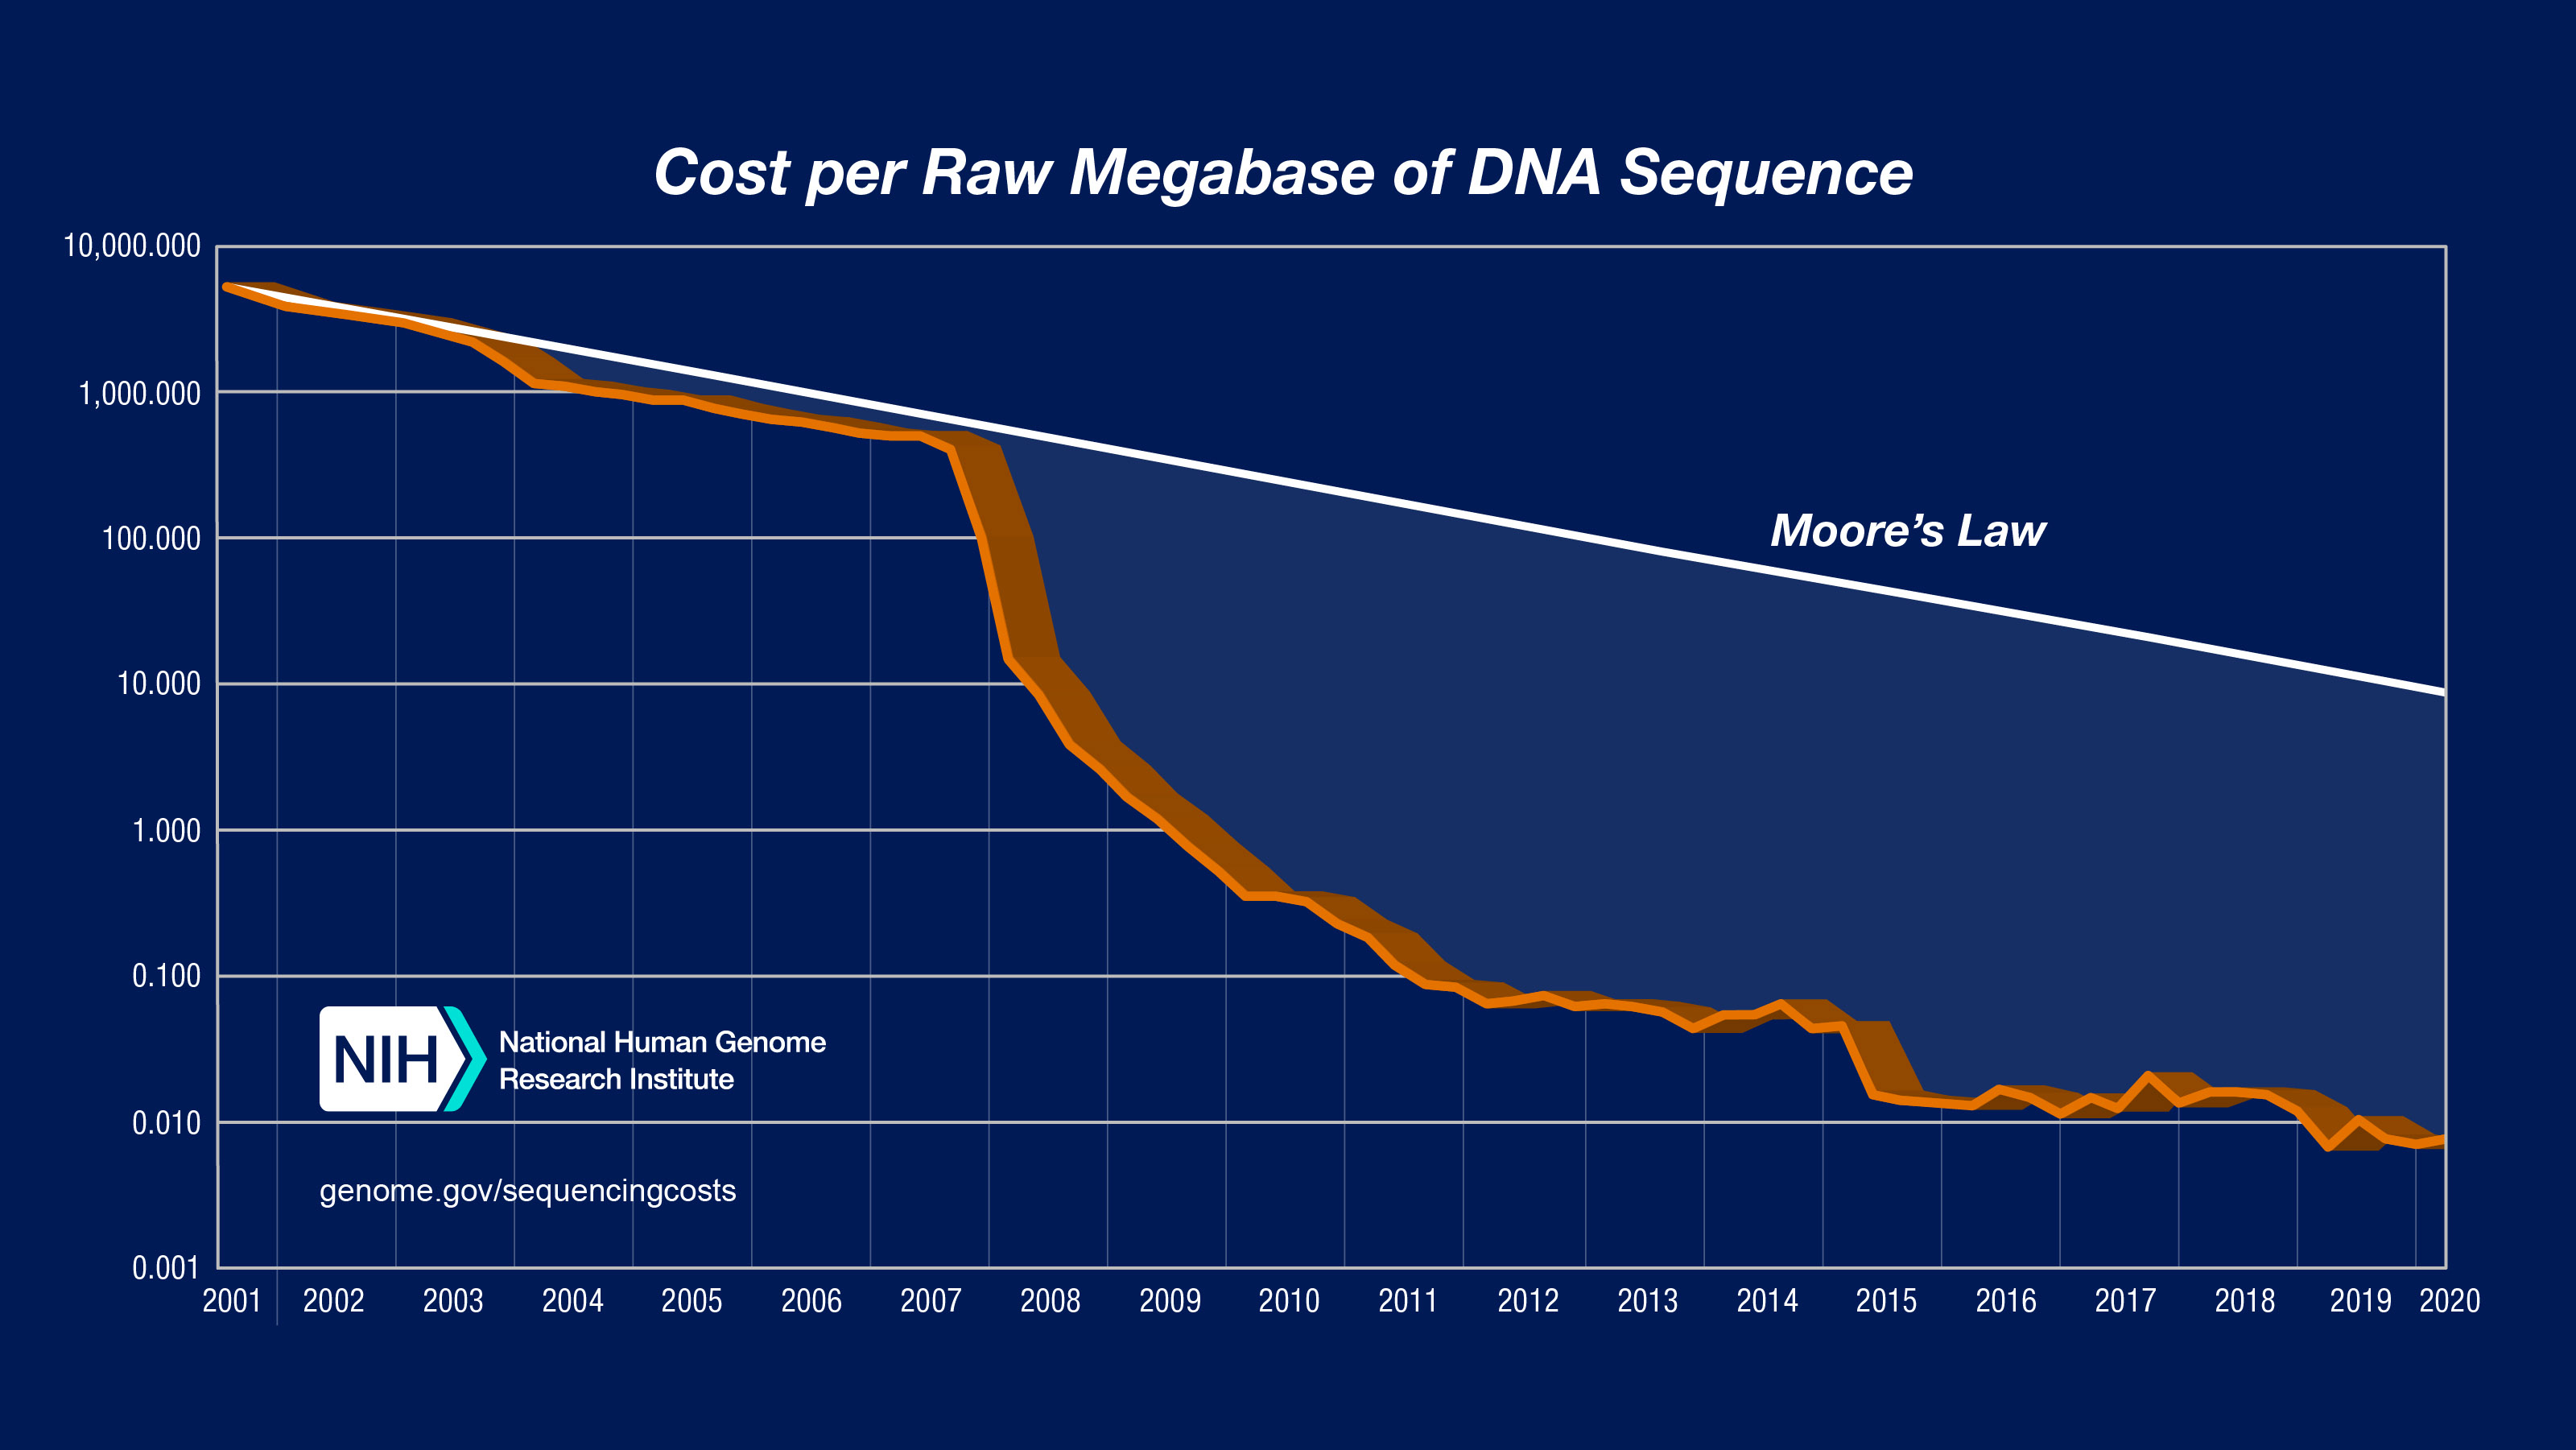
\includegraphics[width=0.9\linewidth]{img/couts} 

}

\caption{Évolution du coût de séquençage (en dollar) d'une mégabase d'ADN, en échelle logarithmique, tiré de \url{www.genome.gov}.}\label{fig:couts}
\end{figure}
\hypertarget{microbiote}{%
\section{Le microbiote intestinal humain}\label{microbiote}}

Même si les développements méthodologiques présentés dans cette thèse ont une portée générale et ne sont pas limités à un type de microbiote en particulier, ils sont effectués avec le microbiote intestinal humain en ligne de mire. Nous présentons ici quelques propriétés de ce microbiote afin que le lecteur prenne conscience de son importance et ait un exemple concret auquel se raccrocher par la suite.

\hypertarget{description}{%
\subsection{Description}\label{description}}

Le tractus gastro-intestinal, ou tube digestif, abrite une communauté microbienne composée d'environ cent mille milliards de micro-organismes pour un poids d'environ \(2~\text{kg}\) (Ley, Peterson, \& Gordon, \protect\hyperlink{ref-ley2006ecological}{2006}). Par abus de langage, on l'appelle le microbiote intestinal. Chez les adultes au mode de vie occidental et en bonne santé, les bactéries appartenant à l'embranchement (\emph{phylum}) des \emph{Firmicutes} représentent plus de \(60~\%\) de la composante bactérienne du microbiote. Si l'on y ajoute celles appartenant aux embranchements des \emph{Actinobacteria} et des \emph{Bacteroidetes}, cette fraction monte à \(90~\%\) (Zhernakova et al., \protect\hyperlink{ref-zhernakova2016population}{2016}).

La variabilité inter-individus reflète principalement des facteurs environnementaux ou comportementaux, qui structurent fortement les flores microbiennes, notamment: le régime alimentaire (David et al., \protect\hyperlink{ref-david2014diet}{2014}), l'âge (O'Toole \& Claesson, \protect\hyperlink{ref-otoole2010gut}{2010}; Yatsunenko et al., \protect\hyperlink{ref-yatsunenko2012human}{2012}) mais aussi la prise d'antibiotiques (Bokulich et al., \protect\hyperlink{ref-bokulich2016antibiotics}{2016}; Palleja et al., \protect\hyperlink{ref-palleja2018recovery}{2018}), la présence d'un animal de compagnie (Kates et al., \protect\hyperlink{ref-kates2020household}{2020}), etc.

\hypertarget{ruxf4le}{%
\subsection{Rôle}\label{ruxf4le}}

Les micro-organismes qui colonisent le tractus gastro-intestinal dégradent les glucides qui n'ont pas été préalablement absorbés par l'hôte (Flint, Scott, Duncan, Louis, \& Forano, \protect\hyperlink{ref-flint2012microbial}{2012}; Rowland et al., \protect\hyperlink{ref-rowland2018gut}{2018}). Ces réactions produisent des acides gras à chaîne courte (AGCC) qui sont des sources d'énergies importantes pour l'humain. Plusieurs voies métaboliques, présentes chez différentes bactéries, permettent de produire des AGCC et il n'existe donc pas un profil unique pour tous les humains. Des études à grande échelles (Arumugam et al., \protect\hyperlink{ref-arumugam2011enterotypes}{2011}) ont cependant permis de dégager des « profils types », appelés entérotypes, caractérisés entre autres par l'alimentation.

Certaines dégradations de sucres effectuées par le microbiote sont inaccessibles aux seules voies métaboliques humaines : le microbiote constitue donc un compagnon indispensable pour assimiler pleinement les nutriments que nous consommons. Citons l'exemple de la population japonaise, qui consomme en moyenne \(14.2~\text{g}\) de nori (un type d'algue) par jour et dans laquelle les enzymes porphyranases et agarases responsables de la dégradation des algues sont produites par la bactérie \emph{Bacteroides plebeius}. Cette capacité a été obtenue à la suite d'un transfert horizontal de gène de la part \emph{Zobellia galactanivorans}, une bactérie marine (Hehemann et al., \protect\hyperlink{ref-hehemann2010transfer}{2010}).

Le système immunitaire doit également beaucoup au microbiote intestinal (Blander, Longman, Iliev, Sonnenberg, \& Artis, \protect\hyperlink{ref-blander2017regulation}{2017}). Parmi les AGCC précédemment cités, on retrouve le butyrate, un métabolite ayant des propriétés anti-inflammatoires et favorisant la prolifération cellulaire au sein de la muqueuse intestinale, ce qui participe à la prévention du cancer colorectal (Canani et al., \protect\hyperlink{ref-canani2011potential}{2011}).
La composition du microbiote intestinal a également un effet sur l'efficacité des vaccins (Valdez, Brown, \& Finlay, \protect\hyperlink{ref-valdez2014influence}{2014}). Eloe-Fadrosh et al. (\protect\hyperlink{ref-eloe2013impact}{2013}) ont mis en évidence que les patients les plus répondeurs pour un vaccin antityphoïdique étaient ceux présentant une proportion plus importante de \emph{Clostridiales}. Mentionnons enfin dans ce domaine, la bactérie \emph{Bacteroides thetaiotamicron} qui induit une production du peptide antimicrobien \(\text{LL-37}\), lequel protège à son tour son hôte contre les infections par \emph{Candida albicans} (Fan et al., \protect\hyperlink{ref-fan2015activation}{2015}).

La signalisation biochimique bidirectionnelle entre le tractus gastro-intestinal et le système nerveux central, communément appelée axe intestin-cerveau, est grandement affectée par le microbiote intestinal. Les résultats les plus spectaculaires sont obtenues chez la drosophile, dans laquelle le microbiote intestinal participe à la modulation des comportements locomoteur (Schretter et al., \protect\hyperlink{ref-schretter2018gut}{2018}) et sexuel (Sharon et al., \protect\hyperlink{ref-sharon2010commensal}{2010}), et chez le rat, dans lequel la production d'un métabolite (l'indole) par certaines bactéries du microbiote induit des troubles du comportement et des troubles de l'anxiété (Jaglin et al., \protect\hyperlink{ref-jaglin2018indole}{2018}).

\hypertarget{dysbioses}{%
\subsection{Dysbioses}\label{dysbioses}}

Le terme dysbiose désigne un déséquilibre du microbiote, qui se traduit généralement par une perte de diversité ou par la surreprésentation d'une espèce. La table \ref{tab:dysbioses} présente un ensemble de maladies qui seraient causées par ou associées à une dysbiose.

\newpage
\begin{longtable}[]{@{}cc@{}}
\caption{\label{tab:dysbioses} Quelques exemples de maladies associées à une dysbiose.}\tabularnewline
\toprule
\begin{minipage}[b]{0.31\columnwidth}\centering
Type de maladie\strut
\end{minipage} & \begin{minipage}[b]{0.63\columnwidth}\centering
Maladie\strut
\end{minipage}\tabularnewline
\midrule
\endfirsthead
\toprule
\begin{minipage}[b]{0.31\columnwidth}\centering
Type de maladie\strut
\end{minipage} & \begin{minipage}[b]{0.63\columnwidth}\centering
Maladie\strut
\end{minipage}\tabularnewline
\midrule
\endhead
\begin{minipage}[t]{0.31\columnwidth}\centering
Maladies métaboliques\strut
\end{minipage} & \begin{minipage}[t]{0.63\columnwidth}\centering
Obésité (Turnbaugh et al., \protect\hyperlink{ref-turnbaugh2009core}{2009})\strut
\end{minipage}\tabularnewline
\begin{minipage}[t]{0.31\columnwidth}\centering
\strut
\end{minipage} & \begin{minipage}[t]{0.63\columnwidth}\centering
Diabète de type 2 (Qin et al., \protect\hyperlink{ref-qin2012metagenome}{2012})\strut
\end{minipage}\tabularnewline
\begin{minipage}[t]{0.31\columnwidth}\centering
\strut
\end{minipage} & \begin{minipage}[t]{0.63\columnwidth}\centering
Cirrhose (Qin et al., \protect\hyperlink{ref-qin2014alterations}{2014})\strut
\end{minipage}\tabularnewline
\begin{minipage}[t]{0.31\columnwidth}\centering
Maladies immunitaires\strut
\end{minipage} & \begin{minipage}[t]{0.63\columnwidth}\centering
Maladie de Crohn (Morgan et al., \protect\hyperlink{ref-morgan2012dysfunction}{2012})\strut
\end{minipage}\tabularnewline
\begin{minipage}[t]{0.31\columnwidth}\centering
\strut
\end{minipage} & \begin{minipage}[t]{0.63\columnwidth}\centering
Syndrome de l'intestin irritable (Chong et al., \protect\hyperlink{ref-chong2019microbiome}{2019})\strut
\end{minipage}\tabularnewline
\begin{minipage}[t]{0.31\columnwidth}\centering
\strut
\end{minipage} & \begin{minipage}[t]{0.63\columnwidth}\centering
Sclérose en plaques (Cekanaviciute et al., \protect\hyperlink{ref-cekanaviciute2017gut}{2017})\strut
\end{minipage}\tabularnewline
\begin{minipage}[t]{0.31\columnwidth}\centering
\strut
\end{minipage} & \begin{minipage}[t]{0.63\columnwidth}\centering
Asthme (Stokholm et al., \protect\hyperlink{ref-stokholm2018maturation}{2018})\strut
\end{minipage}\tabularnewline
\begin{minipage}[t]{0.31\columnwidth}\centering
Maladies psychiatrique\strut
\end{minipage} & \begin{minipage}[t]{0.63\columnwidth}\centering
Dépression (Foster \& Neufeld, \protect\hyperlink{ref-foster2013gut}{2013})\strut
\end{minipage}\tabularnewline
\begin{minipage}[t]{0.31\columnwidth}\centering
\strut
\end{minipage} & \begin{minipage}[t]{0.63\columnwidth}\centering
Schizophrénie (Zheng et al., \protect\hyperlink{ref-zheng2019gut}{2019})\strut
\end{minipage}\tabularnewline
\begin{minipage}[t]{0.31\columnwidth}\centering
Maladies neurologiques\strut
\end{minipage} & \begin{minipage}[t]{0.63\columnwidth}\centering
Maladie d'Alzheimer (Pistollato et al., \protect\hyperlink{ref-pistollato2016role}{2016})\strut
\end{minipage}\tabularnewline
\begin{minipage}[t]{0.31\columnwidth}\centering
\strut
\end{minipage} & \begin{minipage}[t]{0.63\columnwidth}\centering
Maladie de Parkinson (Bedarf et al., \protect\hyperlink{ref-bedarf2017functional}{2017})\strut
\end{minipage}\tabularnewline
\begin{minipage}[t]{0.31\columnwidth}\centering
\strut
\end{minipage} & \begin{minipage}[t]{0.63\columnwidth}\centering
Syndrome de Gilles de La Tourette (Ding et al., \protect\hyperlink{ref-ding2019selective}{2019})\strut
\end{minipage}\tabularnewline
\begin{minipage}[t]{0.31\columnwidth}\centering
Autres maladies\strut
\end{minipage} & \begin{minipage}[t]{0.63\columnwidth}\centering
Eczema (Abrahamsson et al., \protect\hyperlink{ref-abrahamsson2012low}{2012})\strut
\end{minipage}\tabularnewline
\begin{minipage}[t]{0.31\columnwidth}\centering
\strut
\end{minipage} & \begin{minipage}[t]{0.63\columnwidth}\centering
Maladies cardiovasculaires (Kelly et al., \protect\hyperlink{ref-kelly2016gut}{2016})\strut
\end{minipage}\tabularnewline
\begin{minipage}[t]{0.31\columnwidth}\centering
\strut
\end{minipage} & \begin{minipage}[t]{0.63\columnwidth}\centering
Cancer colorectal (Zeller et al., \protect\hyperlink{ref-zeller2014potential}{2014})\strut
\end{minipage}\tabularnewline
\begin{minipage}[t]{0.31\columnwidth}\centering
\strut
\end{minipage} & \begin{minipage}[t]{0.63\columnwidth}\centering
Entérocolite nécrosante (Mai et al., \protect\hyperlink{ref-mai2011fecal}{2011})\strut
\end{minipage}\tabularnewline
\bottomrule
\end{longtable}
\hypertarget{utilisations}{%
\subsection{Utilisations}\label{utilisations}}

Les liens entre microbiote et santé étant très nombreux, la recherche académique ainsi que les départements de recherche et innovation des industries pharmaceutiques et agroalimentaires n'ont pas attendu pour se lancer dans la recherche d'applications et de traitements tirant parti de ces micro-organismes.

Si certaines bactéries sont bénéfiques pour l'organisme, pourquoi ne pas augmenter volontairement leur quantité dans le microbiote ? C'est ce que proposent les approches probiotiques --aussi appelés bioaugmentation-- qui consistent à administrer (le plus souvent par voie orale) des bactéries vivantes et non-pathogènes (Gibson et al., \protect\hyperlink{ref-gibson2017expert}{2017}). Les probiotiques sont majoritairement considérés comme des compléments alimentaires, qui n'ont pas besoin de montrer leur efficacité pour être commercialisés. Des études cliniques prouvent cependant leur efficacité dans certains cas, comme l'utilisation d'un probiotique à base d'une souche de \emph{Bifidobacterium longum} pour diminuer la dépression chez les patients souffrant du syndrome de l'intestin irritable (Pinto-Sanchez et al., \protect\hyperlink{ref-pinto2017probiotic}{2017}).

Plutôt que de fournir directement des souches vivantes, l'approche par prébiotiques fournit des nutriments non digestibles par l'hôte mais stimulant la croissance de certaines bactéries (Gibson et al., \protect\hyperlink{ref-gibson2017expert}{2017}). Si les aliments « riches en fibres » peuvent être considérés comme des prébiotiques, des prébiotiques de synthèse font leur apparition sur le marché. Nestlé a par exemple déposé un brevet sur des prébiotiques à base d'oligosaccharides qui réduisent la présence de \emph{Streptococcus} chez l'enfant dans le but de diminuer le risque d'obésité une fois adulte (Sakwinska, Berger, Zolezzi, \& Holbrook, \protect\hyperlink{ref-sakwinska2017prebiotics}{2017}). Dans le même registre, la baguette « Amibiote » (contraction entre ami et microbiote), issue d'un partenariat entre INRAE et Bridor, contient \(11~\text{g}\) de fibres pour \(100~\text{g}\) de pain (contre \(2.9~\text{g}\) pour une baguette normale) et favorise la croissance de trois bactéries probiotiques.

Pour modifier la composition du microbiote intestinal, la méthode la plus efficace reste la transplantation fécale. Déjà pratiquée en Chine au \(\text{IV}^{\text{e}}\) siècle (Zhang, Luo, Shi, Fan, \& Ji, \protect\hyperlink{ref-zhang2012should}{2012}), la repopulation de l'intestin d'un sujet malade avec le microbiote d'un sujet sain a fait un retour en force en montrant des résultats spectaculaire pour le traitement des infections à \emph{Clostridium difficile} comparé aux thérapies habituelles (prise d'antibiotiques avec ou sans lavement) (Van Nood et al., \protect\hyperlink{ref-nood2013duodenal}{2013}). L'infection à \emph{Clostridium difficile} provoque des diarrhées potentiellement mortelles et se produit chez des patients dont le microbiote intestinal a déjà subi une perte de diversité, laissant la place au pathogène pour se développer.

Si la transplantation fécale pourrait servir de traitement à d'autres maladies, comme le syndrome de Gilles de La Tourette (Ding et al., \protect\hyperlink{ref-ding2019selective}{2019}), ce n'est pas le seul dessein dans lequel l'utilisation de cette technique est possible. Des transplantations fécales autologues peuvent être envisagées dans le cas où une altération du microbiote serait à prévoir. Cette technique a été testée avec succès par la société française MaaT Pharma pour des patients souffrant de leucémie aiguë myéloïde. Leurs selles sont collectées avant la chimiothérapie et une transplantation fécale autologue permet de restaurer un microbiote diversifié comparable à celui présent dans le tractus avant le traitement (Mohty et al., \protect\hyperlink{ref-mohty2018odyssee}{2018}). Une utilisation plus originale en est faite chez les koalas : la transplantation fécale leur permet de diversifier les espèces d'eucalyptus qu'ils sont capables de digérer, ce qui augmente leurs chances de survie alors que leur environnement est menacé (Reardon, \protect\hyperlink{ref-reardon2018faecal}{2018}).

La médiatisation de ces bons résultats a conduit à l'apparition sur les réseaux sociaux de protocoles pour des transplantations fécales « à faire soi-même » (Ekekezie et al., \protect\hyperlink{ref-ekekezie2020understanding}{2020}), y compris pour des indications pour lesquelles elles ne sont (pour l'instant) pas recommandées comme le syndrome de l'intestin irritable ou les troubles de l'autisme. En fonction des pays, la thérapie fécale est considérée comme un médicament ou une transplantation au même titre que les organes.

Plutôt que de modifier le microbiote et d'espérer que la nouvelle composition sera favorable, il est possible d'administrer directement des composés issus des bactéries désirées. C'est sur ce terrain que se place la biotech Enterome, qui a montré que l'administration de peptides issus du microbiote déclenchait une réponse immunitaire capable de s'attaquer à des tumeurs spécifiques (Chene et al., \protect\hyperlink{ref-chene2019microbiome}{2019}).

Une autre façon de tirer parti du microbiome est de s'en servir comme d'un biomarqueur : regarder sa composition peut être un moyen de déceler une maladie sans avoir recours à des tests invasifs ou plus coûteux.
Zeller et al. (\protect\hyperlink{ref-zeller2014potential}{2014}) ont par exemple proposé un modèle prédictif basé principalement sur les abondances de souches de \emph{Fusobacterium nucleatum}, \emph{Porphyromonas asaccharolytica} et \emph{Peptostreptococcus stomatis} pour détecter de façon précoce un cancer colorectal.
Chez les nouveaux-nés, l'entérocolite nécrosante est précédée d'une dysbiose caractéristique (Mai et al., \protect\hyperlink{ref-mai2011fecal}{2011}) permettant de l'identifier et de proposer un traitement adapté avant que la maladie ne leur soit fatale.

Toutes ces opportunités ont incité de nombreuses sociétés à se lancer sur le marché du microbiote dans l'espoir de croissances rapides. Mais le réveil peut être douloureux lorsque les espoirs se fracassent sur le mur de la réalité, comme Seres Therapeutics en a fait les frais. Le 29 juillet 2016, l'annonce de l'échec de la phase II de son probiotique SER-109 contre les infections à \emph{Clostridium difficile} a entraîné une chute du cours de son action près de \(70~\%\) (figure \ref{fig:seres}). L'entreprise a publié un communiqué en janvier 2017 indiquant que cet échec était dû à une erreur de protocole et qu'elle allait par conséquent entamer un essai de phase III, mais cela n'a pas suffi à rassurer les investisseurs.


\begin{figure}

{\centering 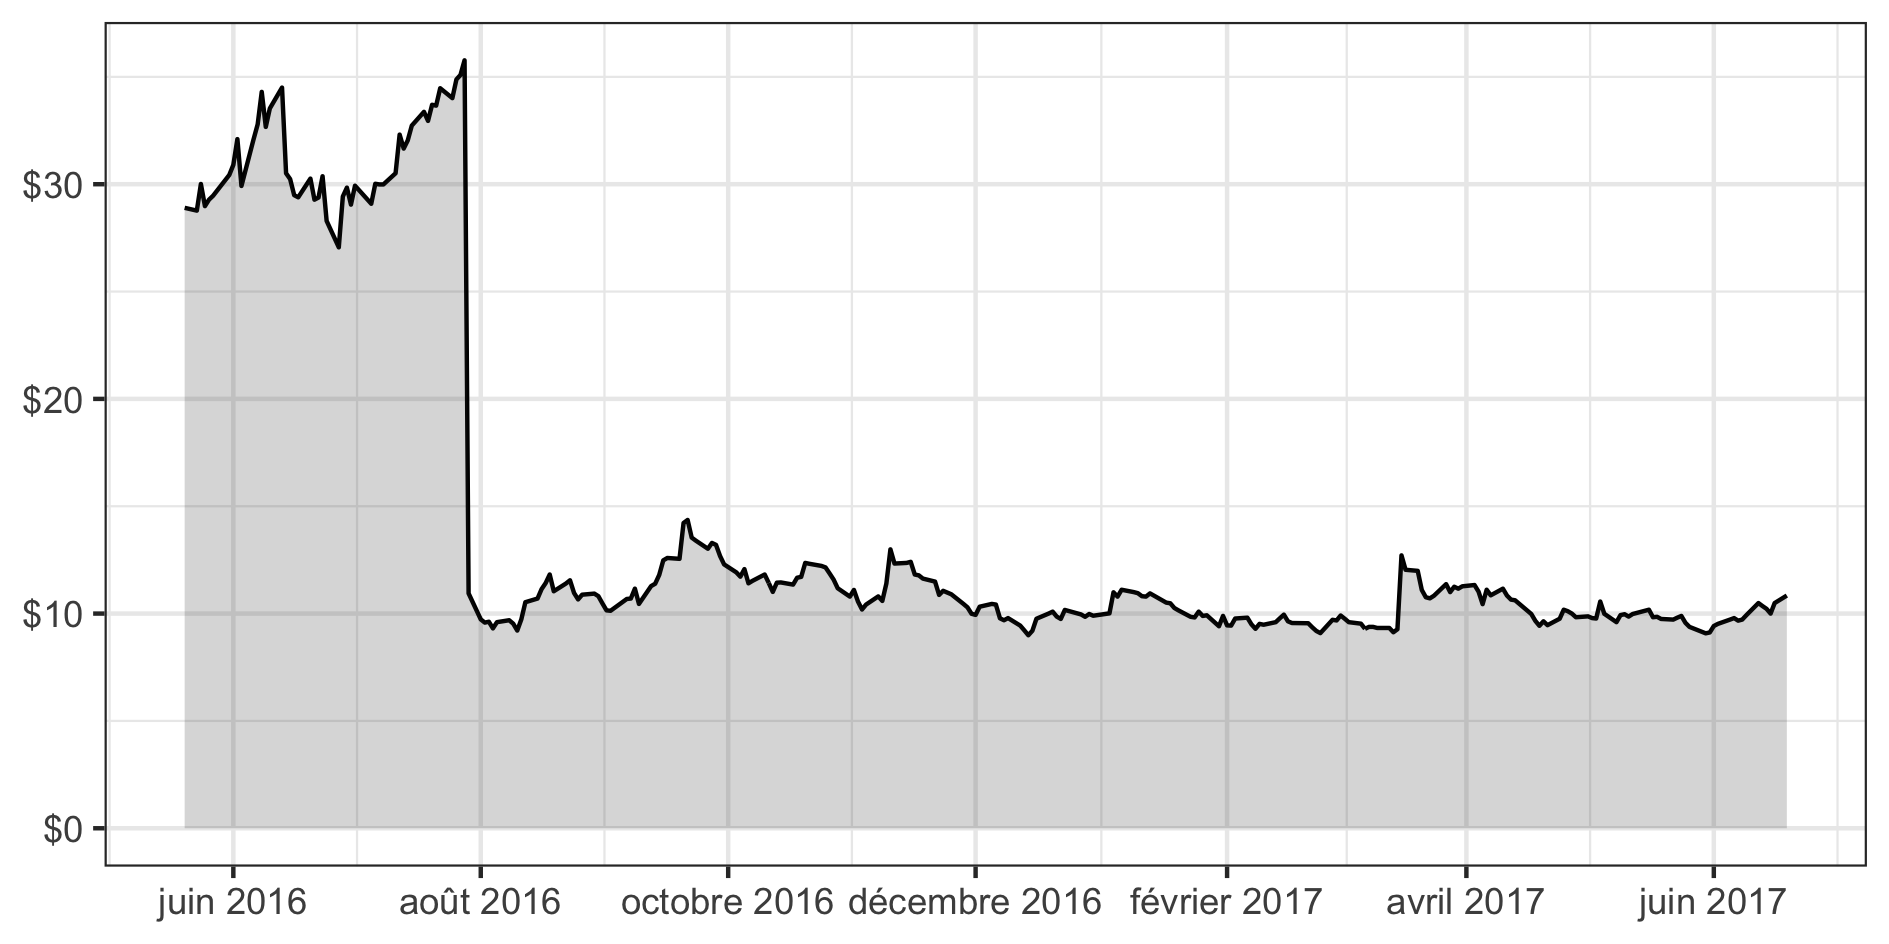
\includegraphics[width=0.9\linewidth]{img/seres} 

}

\caption{Cotation de Seres Therapeutics à partir de l'été 2016.}\label{fig:seres}
\end{figure}
\hypertarget{caracterisation}{%
\section{Caractérisation du microbiote}\label{caracterisation}}

Nous décrivons ici brièvement les différentes méthodes et techniques utilisées pour caractériser le microbiote.

\hypertarget{collecte-des-uxe9chantillons}{%
\subsection{Collecte des échantillons}\label{collecte-des-uxe9chantillons}}

La collecte des échantillons et le mode de conservation des échantillons sont des étapes cruciales pour la reproductibilité des analyses et la fiabilité des résultats. En effet, le temps de stockage avant une congélation à \(-80~^\circ\text{C}\) (Cuthbertson et al., \protect\hyperlink{ref-cuthbertson2014time}{2014}) ou le nombre de dégels successifs (Sergeant, Constantinidou, Cogan, Penn, \& Pallen, \protect\hyperlink{ref-sergeant2012high}{2012}) peuvent avoir un impact important sur la composition microbienne des échantillons, en affectant certains genres plutôt que d'autres.

Il est donc souhaitable d'avoir les conditions les plus homogènes possibles. Cependant, il peut être relativement compliqué d'obtenir des conditions homogènes de collecte et de conservation, notamment quand il s'agit d'études longitudinales où la récolte d'échantillons s'étale sur plusieurs pays ou plusieurs années, avec des équipes différentes, ou bien quand celle-ci est effectuée au domicile du donneur dans le cadre d'études participatives, telles que l'\emph{American Gut Project} (McDonald et al., \protect\hyperlink{ref-mcdonald2018american}{2018}).

\hypertarget{suxe9quenuxe7age-par-guxe8ne-marqueur}{%
\subsection{Séquençage par gène marqueur}\label{suxe9quenuxe7age-par-guxe8ne-marqueur}}

Le séquençage par gène marqueur, en général la sous-unité 16S de l'ARN ribosomique, permet de faire un inventaire taxonomique des espèces présentes dans le microbiote et de répondre à la question « qui est là ? ». Fait notable, le gène codant pour le 16S est présent chez toutes les espèces de bactéries et archées (Kembel, Wu, Eisen, \& Green, \protect\hyperlink{ref-kembel2012incorporating}{2012}). Sa séquence présente une succession de régions conservées, idéales pour l'extraire et l'amplifier par PCR, et des régions hypervariables, qui permettent de déterminer à quel genre (et dans une certaine mesure à quelle espèce) il appartient et de reconstruire une phylogénie. Il bénéficie également de bases de données taxonomiques extrêmement riches (par exemple, SILVA (Quast et al., \protect\hyperlink{ref-quast2012silva}{2012})). Pour toutes ces raisons, le gène 16S est un marqueur idéal pour identifier les différents micro-organismes présents dans un échantillon et quantifier leur abondance (Morgan \& Huttenhower, \protect\hyperlink{ref-morgan2012human}{2012}).

Les différentes étapes d'analyse s'enchaînent comme suit. Après extraction de l'ADN, on amplifie le gène 16S par PCR avec des amorces universelles, calibrées à partir des régions conservées, puis on séquence une ou plusieurs régions hypervariables (pour une longueur totale d'environ 550 paires de bases) par séquençage haut débit. Une fois ces portions d'ADN séquencées, on a accès aux séquences brutes des nucléotides qui les composent, appelées lectures ou \emph{reads}.

Ces lectures doivent ensuite subir un contrôle qualité. En effet, les technologies de séquençage produisent des lectures trop courtes ou de mauvaise qualité (Modolo \& Lerat, \protect\hyperlink{ref-modolo2015urqt}{2015}) qui doivent être éliminées. De plus, lors de l'amplification par PCR, il peut y avoir des évènements d'hybridation entre séquences d'ADN (Meyerhans, Vartanian, \& Wain-Hobson, \protect\hyperlink{ref-meyerhans1990dna}{1990}) qui créent des séquences chimériques et augmentent artificiellement la richesse microbienne. Des algorithmes ont été proposés pour identifier et filtrer les séquences chimériques avant la suite des analyses (Edgar, \protect\hyperlink{ref-edgar2016uchime2}{2016}; Wright, Yilmaz, \& Noguera, \protect\hyperlink{ref-wright2012decipher}{2012}).

Une première approche, dite \emph{affiliation first}, pour identifier à quelles espèces correspondent les lectures séquencés est de trouver une correspondance entre celles-ci et des séquences de références dans des bases de données de gènes 16S comme RDP (Maidak et al., \protect\hyperlink{ref-maidak2000rdp}{2000}, \protect\hyperlink{ref-maidak1997rdp}{1997}), SILVA (Quast et al., \protect\hyperlink{ref-quast2012silva}{2012}) ou Greengenes (DeSantis et al., \protect\hyperlink{ref-desantis2006greengenes}{2006}). Cette méthode est rapide et facilement parallélisable mais rend impossible le regroupement et l'analyse des lectures qui n'ont pas d'homologues dans les bases de référence.

L'approche la plus utilisée, dite \emph{clustering first}, consiste à rassembler les lectures au sein de groupes appelés OTUs, pour \emph{Operational Taxonomic Units}. Ce partitionnement se fait en agglomérant toutes les séquences qui ont au moins \(97~\%\) de similarité de séquence. Des outils bioinformatiques comme Mothur (Schloss et al., \protect\hyperlink{ref-schloss2009introducing}{2009}) ou QIIME (Caporaso et al., \protect\hyperlink{ref-caporaso2010qiime}{2010}) utilisent des algorithmes de classification ascendante hiérarchique pour effectuer ce partitionnement, ce qui est coûteux en calcul et en mémoire. Des algorithmes gloutons (Edgar, \protect\hyperlink{ref-edgar2010search}{2010}) permettent d'accélérer et de réduire l'empreinte mémoire de cette étape de partitionnement. À l'issue de cette étape, un représentant est ensuite choisi pour chaque groupe afin de lui assigner une affiliation taxonomique en comparant ce représentant à des bases de références. Les séquences des représentants permettent également de déterminer un arbre phylogénétique des OTUs. Comparée à l'approche \emph{affiliation first}, l'identification par OTU a l'avantage de pouvoir gérer des espèces non présentes dans les bases de données de référence en les considérant simplement comme mal affiliées. Le microbiote est finalement résumé par une table de comptage \(X = (x_{ij})\) où \(x_{ij}\) correspond au nombre de lectures de l'OTU \(i\) dans l'échantillon \(j\).

Au delà du partitionnement par similarité de séquences, il existe d'autres méthodes pour partitionner l'ensemble des séquences. Mentionnons par exemple le regroupement aux sein d'ASVs, pour \emph{Amplicon Sequence Variants}, qui a vocation à reconstruire les séquences exactes des représentants à l'aide d'un modèle probabiliste des erreurs de séquençage (Callahan, McMurdie, \& Holmes, \protect\hyperlink{ref-callahan2017exact}{2017}; Callahan et al., \protect\hyperlink{ref-callahan2016dada2}{2016}), ou au sein d'oligotypes, qui se focalisent sur les sites nucléotidiques de grande variabilité (Eren, Borisy, Huse, \& Welch, \protect\hyperlink{ref-eren2014oligotyping}{2014}; Eren et al., \protect\hyperlink{ref-eren2013oligotyping}{2013}). Le point de différenciation majeur de ces méthodes par rapport aux OTUs est de ne pas donner le même poids à toutes les positions lors de la construction des groupes de lectures.

La caractérisation par gène marqueur, en particulier le 16S, est bon marché, rapide et s'appuie sur des outils matures. Elle souffre néanmoins de quelques inconvénients :
\begin{enumerate}
\def\labelenumi{\arabic{enumi}.}
\item
  Lors de l'amplification par PCR, outre la possible création de chimères, les taxons très abondants vont avoir plus de chances de voir leurs deux brins s'apparier entre eux plutôt qu'avec une amorce, ce qui brise la chaîne de réplication (Mathieu-Daudé, Welsh, Vogt, \& McClelland, \protect\hyperlink{ref-mathieu1996dna}{1996}). Les taxons peu présents vont au contraire avoir plus de chances d'aller jusqu'au bout de la chaîne de réplication et leur abondance sera surestimée.
\item
  Le nombre de copies du gène 16S varie entre espèces, dans un rapport de \(1\) à \(21\) (Stoddard, Smith, Hein, Roller, \& Schmidt, \protect\hyperlink{ref-stoddard2015rrn}{2015}). Utiliser cette information pour corriger la quantification des OTU améliore l'estimation de la composition microbienne, mais le nombre de copies n'est pas toujours disponible (Kembel et al., \protect\hyperlink{ref-kembel2012incorporating}{2012}), en particulier pour les groupes microbiens peu étudiés.
\item
  Le 16S est limité à la fraction bactérienne du microbiote. D'autres marqueurs comme l'ITS1 et l'ITS2 doivent être utilisées pour la fraction fongique du microbiote. Ces derniers souffrent également du biais du nombre de copies (mais dans un rapport de \(1\) à \(1~000\)) et de bases de référence nettement moins riches.
\item
  Le séquençage par gène marqueur ne permet d'obtenir une résolution taxonomique qu'au niveau du genre, éventuellement de l'espèce dans certains cas favorables. Il ne permet pas non plus de déterminer les fonctions ou voies métaboliques présentes dans le microbiote. Ces dernières peuvent en effet être spécifiques aux souches au sein d'une espèce et nécessitent d'adopter une stratégie non ciblée.
\end{enumerate}

\begin{figure}[!t]

{\centering 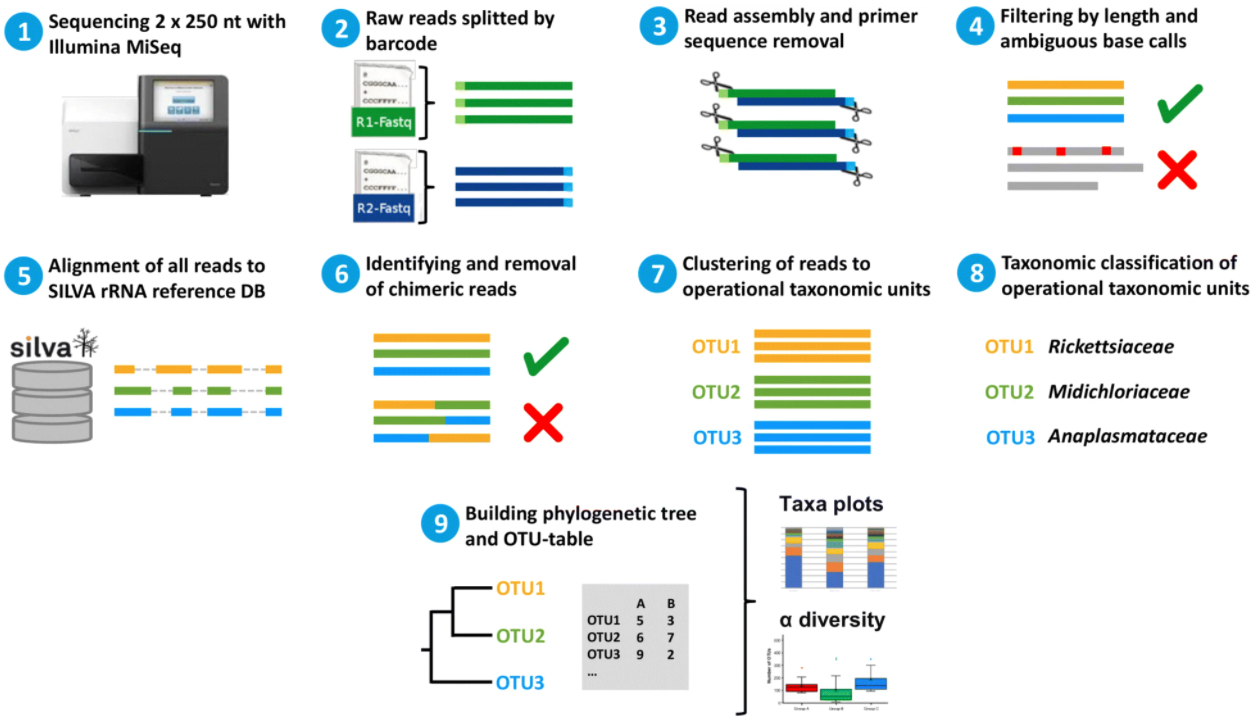
\includegraphics[width=0.9\linewidth]{img/16s} 

}

\caption{Résumé des étapes du séquençage par gène marqueur, tiré de Regier et al. (\protect\hyperlink{ref-regier2019combination}{2019}).}\label{fig:16s}
\end{figure}
\hypertarget{suxe9quenuxe7age-non-cibluxe9}{%
\subsection{Séquençage non ciblé}\label{suxe9quenuxe7age-non-cibluxe9}}

Comme son nom l'indique, le séquençage non ciblé, ou \emph{whole genome shotgun} souvent abrégé en \emph{shotgun}, cible l'ensemble du matériel génétique présent dans les échantillons, et non un unique gène marqueur. Il permet d'étudier le potentiel fonctionnel du microbiote et de répondre à la question « qui peut faire quoi ? ».

On commence par extraire l'ADN contenu dans les cellules puis on le brise par ultrason --ou sonification-- afin d'obtenir de courts fragments, de l'ordre d'une centaine de nucléotides. On effectue ensuite une PCR non ciblée avec des amorces aléatoires pour amplifier les fragments avant de les séquencer pour obtenir des lectures couvrant l'ensemble du matériel génétique.

La construction d'une table de comptage à partir des lectures est sensiblement plus compliquée que dans l'approche par gène marqueur. Il existe en effet plusieurs manières d'obtenir une table de comptage à partir des lectures: par comparaison de lectures (Maillet, Collet, Vannier, Lavenier, \& Peterlongo, \protect\hyperlink{ref-maillet2014commet}{2014}; Maillet, Lemaitre, Chikhi, Lavenier, \& Peterlongo, \protect\hyperlink{ref-maillet2012compareads}{2012}), par comparaison des profils en \(k\)-mers (Benoit et al., \protect\hyperlink{ref-benoit2016multiple}{2016}; Deorowicz, Kokot, Grabowski, \& Debudaj-Grabysz, \protect\hyperlink{ref-deorowicz2015kmc}{2015}), par classification exhaustive des lectures (Brady \& Salzberg, \protect\hyperlink{ref-brady2009phymm}{2009}; Kim, Song, Breitwieser, \& Salzberg, \protect\hyperlink{ref-kim2016centrifuge}{2016}; Ounit, Wanamaker, Close, \& Lonardi, \protect\hyperlink{ref-ounit2015clark}{2015}; Wood \& Salzberg, \protect\hyperlink{ref-wood2014kraken}{2014}), par recensement de gènes marqueurs (Liu, Gibbons, Ghodsi, Treangen, \& Pop, \protect\hyperlink{ref-liu2011accurate}{2011}; Segata et al., \protect\hyperlink{ref-segata2012metagenomic}{2012}; Truong et al., \protect\hyperlink{ref-truong2015metaphlan2}{2015}) ou encore par utilisation d'un catalogue de gènes (Coelho et al., \protect\hyperlink{ref-coelho2019ng}{2019}; Kultima et al., \protect\hyperlink{ref-kultima2012mocat}{2012}; Pons et al., \protect\hyperlink{ref-pons2010meteor}{2010}). Nous allons détailler cette dernière méthode, qui nécessite la construction préalable d'un catalogue ou l'utilisation d'un catalogue public (Almeida et al., \protect\hyperlink{ref-almeida2020unified}{2020}).

Une fois le catalogue obtenu, chaque lecture est alignée contre celui-ci pour déterminer le gène auquel elle correspond le plus, sur la base de la similarité de séquence. Dans le meilleur des cas, une lecture ne s'aligne que sur un seul gène, mais il arrive dans environ \(10~\%\) des cas qu'elle s'aligne sur plusieurs gènes distincts, par exemple parce qu'elle correspond à un domaine protéique partagé par plusieurs séquences. Dans ce dernier cas, plusieurs procédures sont possibles :
\begin{itemize}
\item
  On ne prend pas en compte cette lecture dans le comptage.
\item
  Le compte de cette lecture est réparti uniformément entre les gènes (\emph{i.e.} elle augmente le comptage de chacun des \(n\) gènes sur lesquels elle s'aligne de \(1/n\)).
\item
  Le compte de cette lecture est réparti entre les gènes, au prorata de leurs comptages obtenus à partir des lectures non ambiguës (\emph{i.e.} si elle s'aligne sur les gènes \(G_1, \dots, G_n\) de comptages respectifs \(A_1, \dots, A_n\) dans les lectures non ambiguës, l'abondance du gène \(i\) est augmentée de \(A_i / \sum_{j=1}^n A_j\)).
\end{itemize}
Contrairement à l'approche par gène marqueur, l'approche non-ciblée sur catalogue de gènes dresse un inventaire fonctionnel du microbiote, où le gène remplace l'OTU comme descripteur de base du microbiote.


\begin{figure}

{\centering 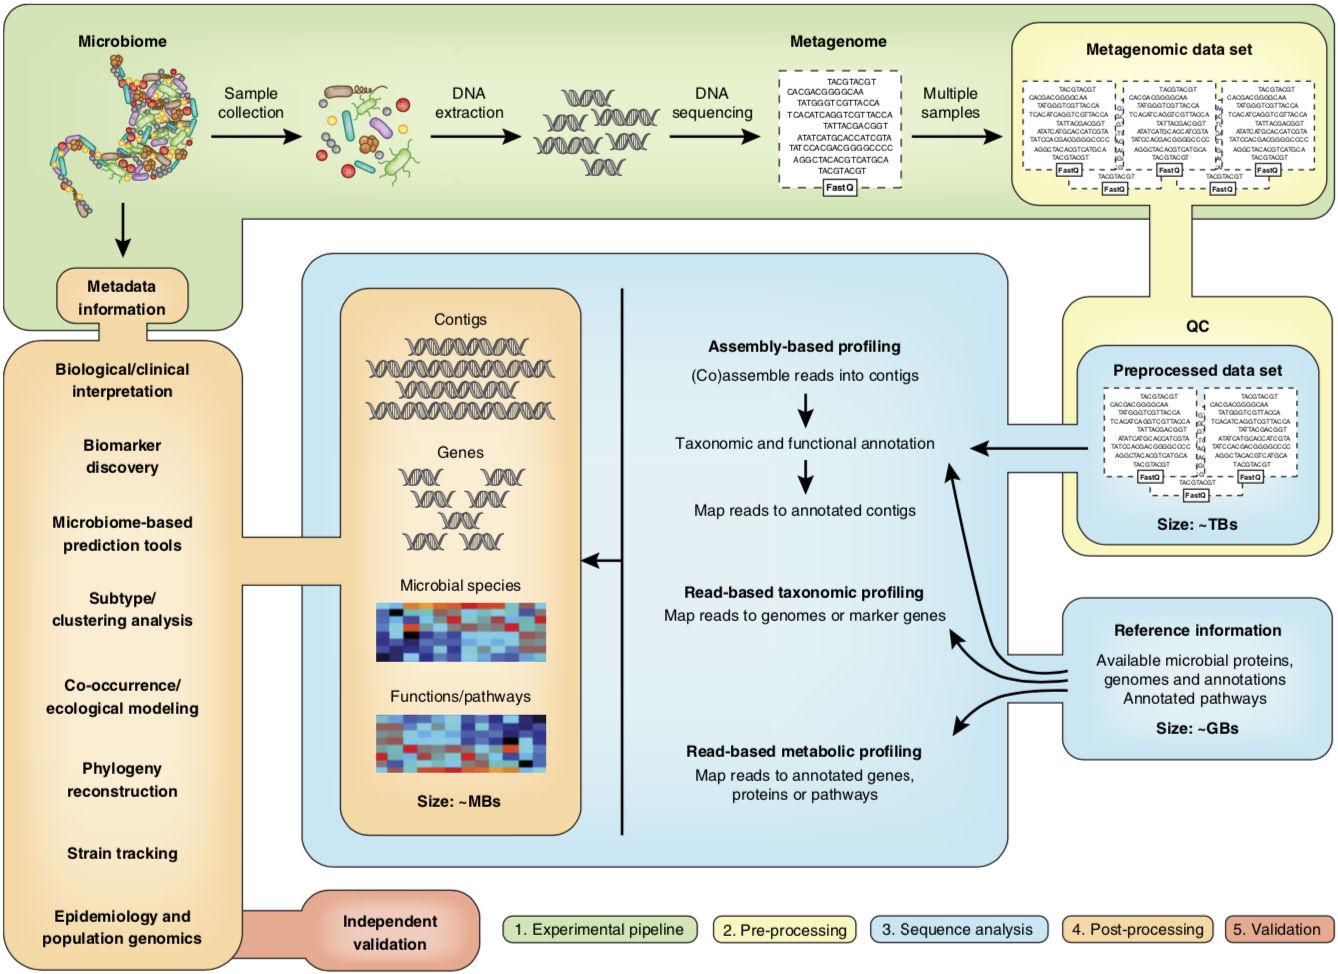
\includegraphics[width=0.9\linewidth]{img/shotgun} 

}

\caption{Résumé des étapes du séquençage non ciblé, tiré de Quince, Walker, Simpson, Loman, \& Segata (\protect\hyperlink{ref-quince2017shotgun}{2017}).}\label{fig:shotgun}
\end{figure}
\hypertarget{donneesmetagenomiques}{%
\subsection{Données métagénomiques}\label{donneesmetagenomiques}}

Une fois l'annotation effectuée, on dispose d'une table de comptage, c'est-à-dire du compte des différentes entités considérées dans les échantillons. Dans la suite, on désignera ces entités sous le terme générique \emph{taxon}, qu'il s'agisse d'espèces, de genres bactériens, d'OTUs, de gènes\ldots{}

Plusieurs cadres conceptuels existent pour analyser ces données mais les deux plus populaires sont ceux (i) des données de comptage et (ii) des données compositionnelles. Chacun de ces cadres possède des avantages et inconvénients qui lui sont propres et malgré des discussions intenses dans la littérature, (Gloor, Macklaim, Pawlowsky-Glahn, \& Egozcue, \protect\hyperlink{ref-gloor2017microbiome}{2017}; Gloor et al., \protect\hyperlink{ref-gloor2016relative}{2016}; McMurdie \& Holmes, \protect\hyperlink{ref-mcmurdie2014waste}{2014}; Vandeputte et al., \protect\hyperlink{ref-vandeputte2017quantitative}{2017}), il n'existe pas à l'heure actuelle de consensus sur celui à privilégier.

\hypertarget{donnuxe9es-de-comptage}{%
\subsubsection*{Données de comptage}\label{donnuxe9es-de-comptage}}
\addcontentsline{toc}{subsubsection}{Données de comptage}

Par la façon dont elles sont construites, à savoir en comptant le nombre de lectures de chaque taxon dans chaque échantillon, les tables d'abondance sont composées de données de comptage, à valeurs dans \(\NN\).

Une approche naturelle serait de considérer ces comptes comme issus d'une loi de Poisson, dont les masses sont telles que \(\PP{X = k} = \frac{\lambda^k}{k!}e^{-\lambda}\) pour \(k \in \NN\). Cependant, l'espérance et la variance d'une loi de Poisson sont égales, alors que les données observées sont surdispersées : elles possèdent une plus grande variabilité qu'attendue pour une distribution de Poisson (Anders \& Huber, \protect\hyperlink{ref-anders2010differential}{2010}; Robinson \& Smyth, \protect\hyperlink{ref-robinson2007moderated}{2007}). Afin de prendre en compte une telle surdispersion dans les données, il est préférable d'utiliser une loi binomiale négative (Zhang et al., \protect\hyperlink{ref-zhang2017negative}{2017}), qui peut être vu comme un mélange de loi de Poisson, avec une densité \(\Gamma\) sur le paramètre de la loi de Poisson.

Dans sa définition classique, la loi binomiale négative de paramètres \(n\) et \(p\) compte le nombre d'échecs avant d'obtenir \(n\) succès pour un événement binaire, avec \(p\) comme probabilité de succès. Sa fonction de répartition est alors telle que
\begin{equation*}
\PP{X = k} = \binom{k+n-1}{n-1} p^n(1-p)^k.
\end{equation*}
On préférera utiliser ici une autre paramétrisation, celle de moyenne \(m\) et de paramètre de dispersion \(\alpha \geq 0\). Lorsque \(\alpha = 0\), on retombe sur une loi de Poisson. Dans le cas contraire,
\begin{equation*}
\PP{X = k} = \frac{\Gamma(k+r)}{k!\Gamma(r)}\left(\frac{m}{r+m}\right)^r\left(\frac{r}{r+m}\right)^k
\end{equation*}
où \(r=\frac{1}{\alpha}\) et \(\Gamma : z \mapsto \int_0^{+\infty}t^{z-1}e^{-t}\dx{t}\) est la fonction gamma.

Une autre particularité des données métagénomiques est leur grande proportion de zéros : les comptages nuls sont surreprésentés et représentent fréquemment \(90~\%\) ou plus des coefficients de la table. Ceux-ci peuvent être des zéros structurels --de nature biologique-- où le taxon n'est pas présent dans le jeu de données, ou des zéros d'échantillonnage --de nature probabiliste-- où le taxon n'a pas été détecté alors qu'il est présent (mais en faible quantité) dans le jeu de données. Pour modéliser cette fréquence élevée de comptages nuls, on utilise alors des lois avec excès de zéros. Si \(X\) suit une loi sur \(\NN\), on peut créer \(Y\) avec excès de zéros comme suit :
\begin{equation*}
\left\{
\begin{aligned}
\PP{Y = 0} & = p_0 + (1-p_0) \PP{X = 0}\\
\PP{Y = k} & = (1-p_0) \PP{X = k} & \text{pour } k\in \NN^*,
\end{aligned}
\right.
\end{equation*}
où \(p_0\) est la proportion de zéros structurels. Si \(X\) suit une loi binomiale négative, \(Y\) suivra alors une loi binomiale négative avec excès de zéros, ou ZINB (pour \emph{Zero-Inflated Negative Binomial}) (Xinyan, Himel, \& Nengjun, \protect\hyperlink{ref-xinyan2016zero}{2016}).

La somme des comptages des taxons dans un échantillon est appelé \emph{profondeur de séquençage} et correspond au nombre de lectures produites par le séquenceur pour l'échantillon. La profondeur \emph{cible} (typiquement \(100~000\) lectures par échantillons) est imposée par le scientifique mais la profondeur \emph{effective} peut varier d'un facteur \(4\) pour des échantillons avec la même cible (\(50~000\) lectures pour le premier, \(200~000\) pour le deuxième).
Il est d'usage d'utiliser un facteur de normalisation pour prendre en compte ces différences et rendre les comptages comparables entre échantillons.

\hypertarget{donnuxe9es-compositionnelles}{%
\subsubsection*{Données compositionnelles}\label{donnuxe9es-compositionnelles}}
\addcontentsline{toc}{subsubsection}{Données compositionnelles}

L'autre grand point de vue considère que les comptages sont contraints par la profondeur de séquençage et ne nous permettent donc d'étudier que les \emph{abondances relatives} (par opposition aux \emph{abondances absolues}) des différents taxons dans l'échantillon. En pratique, les comptages des \(m\) taxons de chaque échantillon sont divisés par la profondeur de séquençage de l'échantillon pour reconstruire des vecteurs d'abondance relative, à valeurs dans le simplexe \(\mathcal{S}^m = \left\{x \in \RR_+^{*,m}, \sum_{i=1}^m x_i = 1 \right\}\) (Gloor \& Reid, \protect\hyperlink{ref-gloor2016compositional}{2016}).

Ces vecteurs de proportion peuvent ensuite être modélisées comme des tirages de lois de Dirichlet. La loi de Dirichlet \(\mathcal{D}(\alpha)\) sur \(\mathcal{S}^m\) de paramètre \(\alpha = (\alpha_1, \ldots, \alpha_m) \in \RR_+^{*,m}\) a pour densité
\begin{equation*}
f(x_1, \ldots, x_m) = \frac{1}{\text{B}(\alpha)} \prod_{i=1}^m x_i^{\alpha_i-1},
\end{equation*}
où \(\text{B} : \alpha \mapsto \frac{\prod_{i=1}^m\Gamma(\alpha_i)}{\Gamma\left(\sum_{i=1}^m \alpha_i\right)}\) est la fonction beta.

Des approches plus sophistiquées, basées sur des lois hiérarchiques multinomiales Dirichlet, permettent de modéliser en plus le fait que les comptages sont une version bruitée du vecteur de proportion (Holmes, Harris, \& Quince, \protect\hyperlink{ref-holmes2012dirichlet}{2012}).
\begin{equation*}
\begin{aligned}
p & \sim \mathcal{D}(\alpha), \\
\PP{X_1 = n_1, \ldots, X_m = n_m\mid p} & = \frac{n!}{\prod_{i=1}^m n_i!}\prod_{i=1}^m p_i^{n_i}.
\end{aligned}
\end{equation*}
\newline

La transformation en proportions préserve certaines propriétés, par exemple le rang d'un taxon au sein d'un échantillon, mais requiert une attention particulière pour d'autres opérations élémentaires, comme le calcul d'une composition moyenne. Aitchison (\protect\hyperlink{ref-aitchison1982statistical}{1982}) est le premier à proposer une géométrie \emph{compositionnelle} du simplexe, qui diffère de la géométrie euclidienne standard. Dans cette géométrie, le simplexe possède ses propres opérations internes de perturbation \(\oplus\) ou de composition \(\odot\) ainsi que sa propre distance \(d_a\) définie par
\begin{equation*}
d_a(x, y) = \sqrt{\frac{1}{2m}\sum_{i=1}^m\sum_{i=1}^m\left(\ln\left(\frac{x_i}{x_j}\right)-\ln\left(\frac{y_i}{y_j}\right)\right)^2} \text{ pour } x,y\in\mathcal{S}^m.
\end{equation*}
\newline

Un point régulièrement évoqué, que la géométrie d'Aitchison corrige, est la présence de corrélations négatives fallacieuses dans le jeu de données normalisé par la somme. Pour s'en convaincre, on peut considérer \(2\) variables indépendantes \(X\), \(Y\) et constater que \(p_1 = \frac{X}{X+Y}\) et \(p_2 = \frac{Y}{X+Y} = 1 - p_1\) sont corrélées négativement. Aitchison propose plusieurs transformations, collectivement appelées \emph{xlr}, pour pour plonger le simplexe dans l'espace euclidien standard et pouvoir ainsi appliquer les méthodes d'analyse multivariée standards aux données compositionnelles (Pawlowsky-Glahn, Egozcue, \& Tolosana Delgado, \protect\hyperlink{ref-pawlowsky2007lecture}{2007}).
\begin{itemize}
\tightlist
\item
  \textbf{Le ratio logarithmique additif} (\emph{additive log-ratio}) (Aitchison, \protect\hyperlink{ref-aitchison1986statistical}{1986})
\end{itemize}
\begin{equation*}
\text{alr}: x \in \mathcal{S}^m \mapsto \left(\ln\left(\frac{x_1}{x_m}\right), \ldots, \ln\left(\frac{x_{m-1}}{x_m}\right) \right) \in \RR^{m-1}.
\end{equation*}
Cette transformation souffre de deux problèmes : elle ne conserve pas les distances entre le simplexe et \(\RR^{m-1}\) et nécessite d'utiliser un taxon de référence (Albarède, \protect\hyperlink{ref-albarede1996introduction}{1996}; Pawlowsky-Glahn et al., \protect\hyperlink{ref-pawlowsky2007lecture}{2007}).
\begin{itemize}
\tightlist
\item
  \textbf{Le ratio logarithmique centré} (\emph{centered log-ratio}) (Aitchison, \protect\hyperlink{ref-aitchison1986statistical}{1986})
\end{itemize}
\begin{equation*}
\text{clr}: x \in \mathcal{S}^m \mapsto \left(\ln\left(\frac{x_1}{g_m(x)}\right), \ldots, \ln\left(\frac{x_{m}}{g_m(x)}\right) \right) \in \RR^{m}
\end{equation*}
où \(g:x\mapsto \sqrt[m]{\prod_{i=1}^m x_i}\) est la fonction de moyenne géométrique.
Bien que cette transformation conserve les distances et ne nécessite plus d'utiliser un taxon de référence, le simplexe est plongé dans un sous-espace vectoriel de dimension \(m-1\) de \(\RR^m\) défini par \(\{y \in \RR^m: y^T 1_m = 0\}\). Autrement dit, la somme des coordonnées du projeté doit être nulle.
\begin{itemize}
\tightlist
\item
  \textbf{Le ratio logarithmique isométrique} (\emph{isometric log-ratio}) (Egozcue, Pawlowsky-Glahn, Mateu-Figueras, \& Barcelo-Vidal, \protect\hyperlink{ref-egozcue2003isometric}{2003}).
\end{itemize}
\begin{equation*}
\text{ilr}: x \in \mathcal{S}^m \mapsto \Psi^T \text{clr}(x) = \left(y_1, \ldots, y_{m-1}\right) \in \RR^{m-1} 
\end{equation*}
où \(\Psi\) est une base orthonormée quelconque du sous-espace vectoriel \(\text{clr}(S^m) = \{y \in \RR^m: y^T 1_m = 0\}\). Cette transformation conserve les distances et nécessite une base adaptée. Un choix classique de base est donné par la matrice de Helmert privée de sa première ligne (et représentée ici pour \(m = 4\))
\begin{equation*}
\Psi^T = 
\begin{pmatrix}
1/\sqrt{2} & -1/\sqrt{2} & 0 & 0 \\
1/\sqrt{6} & 1\sqrt{6}  & -2\sqrt{6} & 0 \\
1/\sqrt{12} & 1\sqrt{12}  & 1\sqrt{12} & -3\sqrt{12} 
\end{pmatrix},
\end{equation*}
pour laquelle on obtient
\begin{equation*}
y_{i-1} = \frac{1}{\sqrt{i(i+1)}} \ln\left(\frac{x_i}{\left(\prod_{j=1}^{i-1} x_j\right)^{\frac{1}{i-1}}}\right) \text{ pour } i \in [\![2,m]\!].
\end{equation*}
Cette base produit des coordonnées \(y_i\) facilement interprétables : \(y_i\) mesure la balance entre \(x_i\) et la moyenne géométrique de \(x_1\) à \(x_{i-1}\).

Si l'on dispose de l'arbre phylogénétique des taxons, d'autres contrastes interprétables peuvent également être utilisés, par exemple la balance entre le sous-arbre gauche et le sous-arbre droit d'un nœud de l'arbre (Silverman, Washburne, Mukherjee, \& David, \protect\hyperlink{ref-silverman2017phylogenetic}{2017}).

Enfin, Xia, Sun, \& Chen (\protect\hyperlink{ref-xia2018statistical}{2018}) proposent une autre base, qui donne les coordonnées suivantes.
\begin{equation*}
y_i = \frac{1}{\sqrt{i(i+1)}}\ln \left(\frac{\prod_{j=1}^i x_j}{(x_i + 1)^i}\right) \text{ pour } i \in [\![1,m-1]\!].
\end{equation*}
\newline

Les transformations xlr ne tolèrent pas des proportions nulles. La solution généralement adoptée consiste à ajouter un pseudo-compte de \(1\) (ou \(1/2\)) à tous les taxons avant de calculer les proportions. Cette solution, si elle permet en pratique de s'abstraire des zéros lors des calculs, présente néanmoins l'inconvénient majeur d'induire des pics dans la densité des coordonnées transformées sans pour autant permettre de gérer explicitement les zéros structurels.

\hypertarget{jeuxdonnees}{%
\section{Jeux de données}\label{jeuxdonnees}}

Nous présentons ici les jeux de données utilisés dans ce manuscrit. Chaque jeu de données porte le nom du premier auteur de l'étude dont il est extrait. Tous sont disponibles dans le matériel supplémentaire de l'article d'origine ou dans le \emph{package} R \texttt{\{curatedMetagenomicData\}} qui met à disposition de manière homogène des jeux de données de métagénomique (Pasolli et al., \protect\hyperlink{ref-pasolli2017accessible}{2017}; R Core Team, \protect\hyperlink{ref-r2020}{2020}). Afin de limiter le bruit lié aux taxons très peu présents dans les jeux de données, ceux-ci pourront être retirés si leur prévalence (\emph{i.e.} le pourcentage d'échantillons dans lesquels le taxon est présent) est en dessous d'un certain seuil.

\hypertarget{brito}{%
\subsubsection*{Brito}\label{brito}}
\addcontentsline{toc}{subsubsection}{Brito}

Brito et al. (\protect\hyperlink{ref-brito2016mobile}{2016}) comparent une cohorte de \(81\) Nord-Américains urbains avec une cohorte de \(171\) Fidjiens ruraux en utilisant à la fois du séquençage 16S (que nous utiliserons) et du séquençage non ciblé. Leurs travaux ont montré que la variation du régime alimentaire se reflète dans la variation du potentiel fonctionnel des gènes du microbiote, les Fidjiens ayant par exemple plus de gènes spécialisés dans la dégradation de l'amidon. En ne gardant que les \(112\) adultes fidjiens de cette cohorte pour former un groupe d'échantillons homogènes, il reste \(77\) OTUs.

\hypertarget{chaillou}{%
\subsubsection*{Chaillou}\label{chaillou}}
\addcontentsline{toc}{subsubsection}{Chaillou}

L'étude de Chaillou et al. (\protect\hyperlink{ref-chaillou2015origin}{2015}) s'intéresse au microbiote alimentaire de produit carnés (bœuf haché, veau haché, merguez de volaille et dés de lardons) et de produits issus de la mer (filet de cabillaud, crevette, filet saumon et saumon fumé) pour étudier le rôle du microbiote dans l'altération de l'aliment. Les \(64\) échantillons, répartis uniformément entre les différents aliments, ont mis en évidence une perte de diversité microbienne concomitante à l'altération et ont permis d'identifier des espèces associées à une altération précoce. En ne conservant que les taxons ayant une prévalence supérieure à \(5~\%\) de prévalence, on conserve \(499\) OTUs dont \(97\) assignées à l'embranchement des \emph{Bacteroidetes}.

\hypertarget{chlamydiae}{%
\subsubsection*{Chlamydiae}\label{chlamydiae}}
\addcontentsline{toc}{subsubsection}{Chlamydiae}

Seule exception à notre terminologie, le jeu de donnée Chlamydiae constitue une sous-partie du jeu de données construit par Caporaso et al. (\protect\hyperlink{ref-caporaso2011global}{2011}). Ce dernier contient \(26\) échantillons répartis au sein de \(8\) environnements très différents (selles, bouche, eau, sol, sédiments, océan, eau douce calme et eau douce vive) pour étudier la diversité microbienne globale et calibrer l'effort de séquençage nécessaire à une bonne caractérisation. Le sous-jeu de données est restreint aux \(21\) OTUs assignées à l'ordre des \emph{Chlamydiales} et a servi d'exemple pour \texttt{\{StructSSI\}} dans Sankaran \& Holmes (\protect\hyperlink{ref-sankaran2014structssi}{2014}).

\hypertarget{ravel}{%
\subsubsection*{Ravel}\label{ravel}}
\addcontentsline{toc}{subsubsection}{Ravel}

Le jeu de données présenté dans Ravel et al. (\protect\hyperlink{ref-ravel2011vaginal}{2011}) concerne le microbiote vaginal de \(396\) femmes nord-américaines, n'ayant pas atteint la ménopause, issues de différents groupes ethniques et sujettes ou non à des vaginoses. Le séquençage par gène marqueur 16S a permis d'identifier cinq \emph{archétypes} de communautés microbiennes: quatre d'entre eux sont dominés par une espèce de \emph{Lactobacillus} qui acidifie le milieu et empêche le développement de bactéries responsables de vaginose, le dernier correspond à une diversité bactérienne élevée et est associé à des risques accrus de vaginose. \(40\) genres différents, de prévalence supérieure à \(5~\%\) sont présents dans ce jeu de données.

\hypertarget{wu}{%
\subsubsection*{Wu}\label{wu}}
\addcontentsline{toc}{subsubsection}{Wu}

Wu et al. (\protect\hyperlink{ref-wu2011linking}{2011}) se sont intéressés aux relations entre microbiote et régime alimentaire, parmi lesquelles l'importance de la consommation d'alcool. Bien qu'un changement de régime alimentaire pendant une courte durée (\(10\) jours) ait un impact significatif sur le microbiote, son ampleur reste modeste. Ce jeu de données, qui comprend \(98\) échantillons répartis à égalité entre sujets à faible et forte consommation d'alcool, contient \(400\) OTUs.

\hypertarget{zeller}{%
\subsubsection*{Zeller}\label{zeller}}
\addcontentsline{toc}{subsubsection}{Zeller}

Le jeu de données issu de Zeller et al. (\protect\hyperlink{ref-zeller2014potential}{2014}) contient \(42\) patients ayant un adénome, \(91\) patients ayant un cancer colorectal et \(66\) volontaires sains. Le but de l'étude est d'étudier les associations entre la composition du microbiote et le statut du patient, notamment pour trouver des biomarqueurs de la maladie. Tous les échantillons ont été caractérisés par l'approche gène marqueur (à l'aide du gène 16S) et par l'approche non-ciblée. En ne conservant que les taxons ayant une prévalence supérieure à \(~5\%\), l'approche gène marqueur a permis d'identifier \(119\) genres différents tandis que l'approche non-ciblée a identifié \(878\) MSPs --une autre entité métagénomique (Plaza Oñate et al., \protect\hyperlink{ref-plaza2018mspminer}{2018}).

\newpage
\begin{longtable}[]{@{}ccccc@{}}
\caption{\label{tab:datasets} Jeux de données utilisés dans ce manuscrit.}\tabularnewline
\toprule
\begin{minipage}[b]{0.29\columnwidth}\centering
Jeu de données\strut
\end{minipage} & \begin{minipage}[b]{0.18\columnwidth}\centering
Microbiote\strut
\end{minipage} & \begin{minipage}[b]{0.10\columnwidth}\centering
Rang\strut
\end{minipage} & \begin{minipage}[b]{0.12\columnwidth}\centering
Taxons\strut
\end{minipage} & \begin{minipage}[b]{0.16\columnwidth}\centering
Échantillons\strut
\end{minipage}\tabularnewline
\midrule
\endfirsthead
\toprule
\begin{minipage}[b]{0.29\columnwidth}\centering
Jeu de données\strut
\end{minipage} & \begin{minipage}[b]{0.18\columnwidth}\centering
Microbiote\strut
\end{minipage} & \begin{minipage}[b]{0.10\columnwidth}\centering
Rang\strut
\end{minipage} & \begin{minipage}[b]{0.12\columnwidth}\centering
Taxons\strut
\end{minipage} & \begin{minipage}[b]{0.16\columnwidth}\centering
Échantillons\strut
\end{minipage}\tabularnewline
\midrule
\endhead
\begin{minipage}[t]{0.29\columnwidth}\centering
Brito et al. (\protect\hyperlink{ref-brito2016mobile}{2016})\strut
\end{minipage} & \begin{minipage}[t]{0.18\columnwidth}\centering
Intestinal\strut
\end{minipage} & \begin{minipage}[t]{0.10\columnwidth}\centering
OTU\strut
\end{minipage} & \begin{minipage}[t]{0.12\columnwidth}\centering
77\strut
\end{minipage} & \begin{minipage}[t]{0.16\columnwidth}\centering
112\strut
\end{minipage}\tabularnewline
\begin{minipage}[t]{0.29\columnwidth}\centering
Chaillou et al. (\protect\hyperlink{ref-chaillou2015origin}{2015})\strut
\end{minipage} & \begin{minipage}[t]{0.18\columnwidth}\centering
Alimentaire\strut
\end{minipage} & \begin{minipage}[t]{0.10\columnwidth}\centering
OTU\strut
\end{minipage} & \begin{minipage}[t]{0.12\columnwidth}\centering
499/97\strut
\end{minipage} & \begin{minipage}[t]{0.16\columnwidth}\centering
64\strut
\end{minipage}\tabularnewline
\begin{minipage}[t]{0.29\columnwidth}\centering
Chlamydiae\strut
\end{minipage} & \begin{minipage}[t]{0.18\columnwidth}\centering
Varié\strut
\end{minipage} & \begin{minipage}[t]{0.10\columnwidth}\centering
OTU\strut
\end{minipage} & \begin{minipage}[t]{0.12\columnwidth}\centering
21\strut
\end{minipage} & \begin{minipage}[t]{0.16\columnwidth}\centering
26\strut
\end{minipage}\tabularnewline
\begin{minipage}[t]{0.29\columnwidth}\centering
(Caporaso et al., \protect\hyperlink{ref-caporaso2011global}{2011})\strut
\end{minipage} & \begin{minipage}[t]{0.18\columnwidth}\centering
\strut
\end{minipage} & \begin{minipage}[t]{0.10\columnwidth}\centering
\strut
\end{minipage} & \begin{minipage}[t]{0.12\columnwidth}\centering
\strut
\end{minipage} & \begin{minipage}[t]{0.16\columnwidth}\centering
\strut
\end{minipage}\tabularnewline
\begin{minipage}[t]{0.29\columnwidth}\centering
Ravel et al. (\protect\hyperlink{ref-ravel2011vaginal}{2011})\strut
\end{minipage} & \begin{minipage}[t]{0.18\columnwidth}\centering
Vaginal\strut
\end{minipage} & \begin{minipage}[t]{0.10\columnwidth}\centering
Genre\strut
\end{minipage} & \begin{minipage}[t]{0.12\columnwidth}\centering
40\strut
\end{minipage} & \begin{minipage}[t]{0.16\columnwidth}\centering
396\strut
\end{minipage}\tabularnewline
\begin{minipage}[t]{0.29\columnwidth}\centering
Wu et al. (\protect\hyperlink{ref-wu2011linking}{2011})\strut
\end{minipage} & \begin{minipage}[t]{0.18\columnwidth}\centering
Intestinal\strut
\end{minipage} & \begin{minipage}[t]{0.10\columnwidth}\centering
OTU\strut
\end{minipage} & \begin{minipage}[t]{0.12\columnwidth}\centering
400\strut
\end{minipage} & \begin{minipage}[t]{0.16\columnwidth}\centering
98\strut
\end{minipage}\tabularnewline
\begin{minipage}[t]{0.29\columnwidth}\centering
Zeller et al. (\protect\hyperlink{ref-zeller2014potential}{2014})\strut
\end{minipage} & \begin{minipage}[t]{0.18\columnwidth}\centering
Intestinal\strut
\end{minipage} & \begin{minipage}[t]{0.10\columnwidth}\centering
Genre\strut
\end{minipage} & \begin{minipage}[t]{0.12\columnwidth}\centering
119\strut
\end{minipage} & \begin{minipage}[t]{0.16\columnwidth}\centering
199\strut
\end{minipage}\tabularnewline
\begin{minipage}[t]{0.29\columnwidth}\centering
Zeller et al. (\protect\hyperlink{ref-zeller2014potential}{2014})\strut
\end{minipage} & \begin{minipage}[t]{0.18\columnwidth}\centering
Intestinal\strut
\end{minipage} & \begin{minipage}[t]{0.10\columnwidth}\centering
MSP\strut
\end{minipage} & \begin{minipage}[t]{0.12\columnwidth}\centering
878\strut
\end{minipage} & \begin{minipage}[t]{0.16\columnwidth}\centering
199\strut
\end{minipage}\tabularnewline
\bottomrule
\end{longtable}
\hypertarget{anadiff}{%
\chapter{Études d'analyse différentielle}\label{anadiff}}

Ce chapitre est un chapitre bibliographique sur les méthodes d'analyses différentielles existantes.
\begin{center}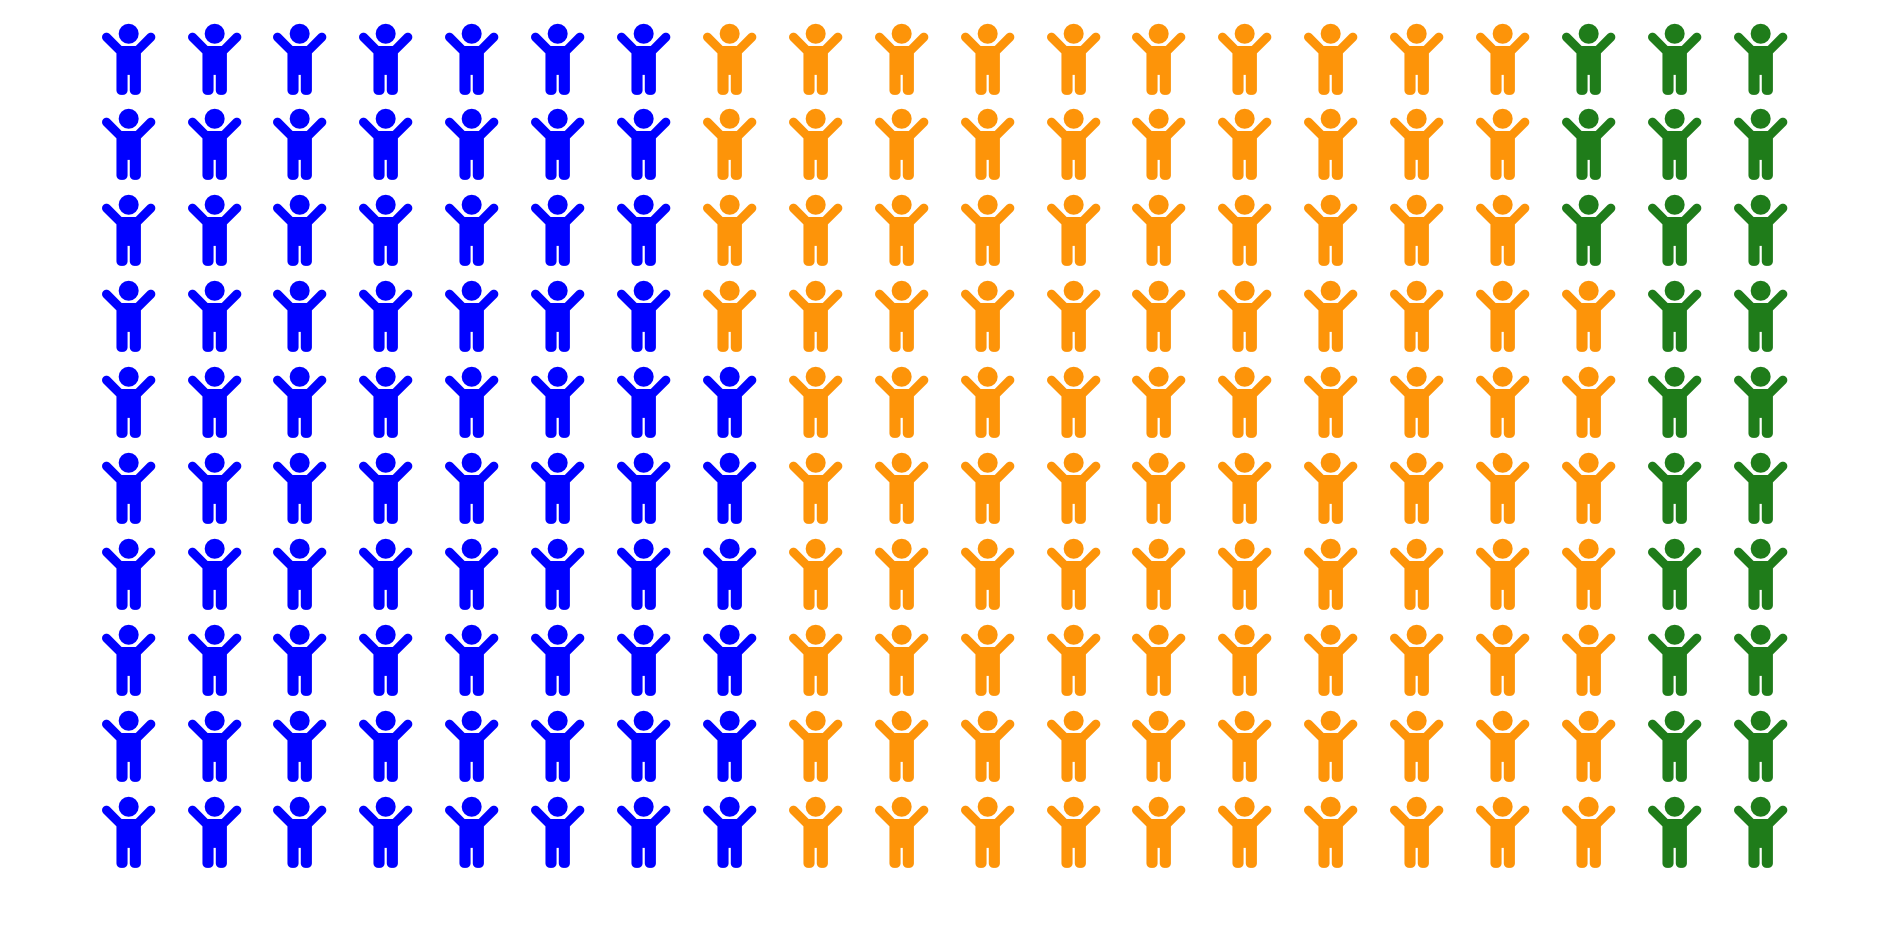
\includegraphics[width=0.9\linewidth]{img/cohort} \end{center}

\hypertarget{tests-statistiques}{%
\section{Tests statistiques}\label{tests-statistiques}}

\hypertarget{analyse-de-la-variance-uxe0-un-facteur}{%
\subsection{Analyse de la variance à un facteur}\label{analyse-de-la-variance-uxe0-un-facteur}}

Une première approche pour tester s'il y a un effet du groupe sur l'abondance est d'utiliser un modèle d'ANOVA à un facteur.

Avec \(k\) groupes, on renumérote les abondances des \(N\) individus tels que \(y_{i,j}\) soit l'abondance du \(j^{\text{ème}}\) individu au sein \(i^{\text{ème}}\) groupe. Avec \(n_i\) individus dans le groupe \(i\), la moyenne des abondances au sein du groupe est \(y_{i,\bullet} = \frac{1}{n_i}\sum_{j = 1}^{n_1} y_{i,j}\) et la moyenne générale est \(y_{\bullet, \bullet} = \frac{1}{N} \sum_{i=1}^k \sum_{j = 1}^{n_i} y_{i,j}\).

Sous les hypothèses de normalité et d'homoscédasticité des résidus, la statistique de test \(F\), définie par
\begin{equation*}
F = \frac{\sum_{i = 1}^k n_i \left(y_{i,\bullet} - y_{\bullet, \bullet} \right)^2 / (k - 1)}{\sum_{i=1}^k \sum_{j = 1}^{n_i} \left(y_{i,j} - y_{i,\bullet} \right)^2 / (N - k)},
\end{equation*}
suit une loi de Fisher à \(k - 1\) et \(N - k\) degrés de liberté.

\(F\) correspond au ratio entre la variance des moyennes de chaque groupe et la variance totale. On rejette alors \(\mathcal{H}_0 = \left\{\text{tous les groupes ont la même moyenne}\right\}\) si \(F\) est suffisamment grande et on considère que le groupe a une influence sur l'abondance.

\hypertarget{test-de-wilcoxon}{%
\subsection{Test de Wilcoxon}\label{test-de-wilcoxon}}

Le test de Wilcoxon-Mann-Whitney (Mann \& Whitney, \protect\hyperlink{ref-mann1947test}{1947}; Wilcoxon, \protect\hyperlink{ref-wilcoxon1992individual}{1992}) permet de tester si, pour deux échantillons, la probabilité qu'une valeur tirée au hasard dans un échantillon soit plus petite qu'une valeur tirée au hasard dans le second est égale à la probabilité qu'elle soit plus grande.
L'hypothèse nulle est alors \(\mathcal{H}_0 = \left\{\PP{X < Y} = \PP {Y < X} \right\}\) pour \(X\) et \(Y\) tirés dans chacune des populations.
En pratique, on utilise ce test non-paramétrique pour vérifier si les deux populations suivent la même distribution ou non.

Formellement, soit \(X = (x_1, \ldots, x_{n_1})\) et \(Y = (y_1, \ldots, y_{n_2})\) les deux échantillons à comparer pour lesquels il n'y a pas d'égalité dans leurs valeurs. Il est possible de définir sans ambiguïté le rang de chaque individu au sein de l'échantillon concaténé de taille \(n_1 + n_2\), puis \(R_1\) la somme des rangs des individus du premier groupe. Sous \(\mathcal{H}_0\), la statistique de test
\begin{equation*}
U = R_1 - \frac{n_1(n_1 + 1)}{2}
\end{equation*}
suit asymptotiquement une loi normale de moyenne \(\frac{n_1n_2}{2}\) et de variance \(\frac{n_1 n_2(n_1 + n_2 + 1)}{12}\). On rejette \(\mathcal{H}_0\) lorsque \(\left|U\right| > \Phi^{-1}(1-\alpha)\).
Il est possible de généraliser lorsqu'il y a des égalités dans les valeurs au sein d'un échantillon ou entre les échantillons. Dans ce cas là, la variance de la loi asymptotique doit être ajustée en conséquence.

\hypertarget{test-de-kruskall-wallis}{%
\subsection{Test de Kruskall-Wallis}\label{test-de-kruskall-wallis}}

Le test de Kruskall-Wallis (Kruskal \& Wallis, \protect\hyperlink{ref-kruskal1952use}{1952}) est une généralisation à \(k\) groupes du test de Wilcoxon-Mann-Whitney. Il est utilisé pour déterminer si les \(k\) échantillons proviennent d'une même population ou si au moins un des échantillons a une distribution différente des autres.

Comme pour Wilcoxon-Mann-Whitney, on commence par concaténer les \(N = \sum_{i = 1}^{k}n_i\) observations des \(k\) échantillons puis calculer la somme des rangs au sein de chaque groupe : \(R_1, \ldots, R_k\). Si les observations sont indépendantes et qu'il n'y a pas d'égalité dans leurs valeurs, la statistique de test
\begin{equation}
\label{eq:hkw}
H = \frac{12}{N (N + 1)} \sum_{i=1}^{k} \frac{R_i^2}{n_i} - 3(N + 1)
\end{equation}
suit une loi du \(\chi^2\) à \(k - 1\) degrés de libertés. \(H\) peut être réécrite comme
\begin{equation*}
\frac{N - 1}{N} \frac{ \sum_{i=1}^k n_i \left(\frac{R_i}{n_i} - \frac{N + 1}{2}\right)^2}{\frac{N^2-1}{12}},
\end{equation*}
qui, à un facteur multiplicatif près, correspond à la statistique de test d'une ANOVA à un facteur sur les rangs et où la variance au dénominateur n'a pas besoin d'être estimée (il s'agit de la variance de la loi uniforme sur \([\![1,N]\!]\)).

Lorsque des égalités sont présentes au sein des échantillons, \(H\) est calculée en divisant l'expression \eqref{eq:hkw} par
\begin{equation*}
1-\frac{\sum_{i = 1}^k t_i^3 - t_i}{N^3 - N},
\end{equation*}
où \(t_i\) est le nombre d'égalités au sein du \(i^{\text{ème}}\) échantillon. Après cette correction, si les \(n_i\) ne sont pas trop petits, cette nouvelle statistique \(H\) corrigée suit toujours une loi qui \(\chi^2\) à \(k - 1\) degrés de liberté.

On rejette l'hypothèse nulle sur l'égalité des rangs moyens \(\mathcal{H}_0 = \left\{ \frac{R_1}{n_1} = \ldots = \frac{R_k}{n_k} \right\}\) lorsque \(H\) est plus grande que la valeur seuil déterminée par \(\alpha\).

\hypertarget{autres-methodes}{%
\subsection{Autres méthodes}\label{autres-methodes}}

Les données métagénomiques ayant les spécificités précédemment présentées dans la section \ref{donneesmetagenomiques} (non-normalité, surabondance de zéros, somme contrainte\ldots), des méthodes spécifiques ont été développées pour les appréhender. Nous pouvons par exemple citer \emph{edgeR} (Robinson, McCarthy, \& Smyth, \protect\hyperlink{ref-robinson2010edger}{2010}), \emph{DESeq2} (Love, Huber, \& Anders, \protect\hyperlink{ref-love2014moderated}{2014}), \emph{metagenomeSeq} (Paulson, Stine, Bravo, \& Pop, \protect\hyperlink{ref-paulson2013differential}{2013}) ou \emph{mbzinb} (Chen et al., \protect\hyperlink{ref-chen2018omnibus}{2018}). Celles-ci peuvent utiliser des modèles linéaires généralisés ou des modèles avec excès de zéros pour essayer d'appréhender au mieux les données.

Nous n'avons pas testé ces méthodes dans nos analyses. Nous nous intéressons à l'apport de l'information hiérarchique et avons préféré utiliser le même test classique (Wilcoxon ou Kruskall-Wallis) dans toutes nos comparaisons. La nouvelle procédure que nous proposons dans le chapitre \ref{nouvelleapproche} peut cependant être appliquée sur les sorties de méthodes quelconques, pourvu qu'elles fournissent un vecteur de \(p\)-valeurs.

\hypertarget{edger-et-deseq2}{%
\subsubsection*{\texorpdfstring{\emph{edgeR} et \emph{DESeq2}}{edgeR et DESeq2}}\label{edger-et-deseq2}}
\addcontentsline{toc}{subsubsection}{\emph{edgeR} et \emph{DESeq2}}

Proposés initialement pour de l'analyse de données de transcriptomique, \emph{edgeR} (Robinson et al., \protect\hyperlink{ref-robinson2010edger}{2010}) et \emph{DESeq2} (Love et al., \protect\hyperlink{ref-love2014moderated}{2014}) ajustent un modèle de régression linéaire généralisé avec une structure d'erreur binomiale négative, afin de prendre en compte la surdispersion des données.

Le compte du taxon \(i\) dans l'échantillon \(j\) appartenant au groupe \(g\) est modélisé par
\begin{equation*}
Y_{i,j} \sim \text{NB}\left(s_j \mu_{i,g},\alpha_{i,g}\right)
\end{equation*}
où \(s_j\) est un facteur de normalisation qui modélise le nombre total de lectures dans l'échantillon \(j\), \(\mu_{i,g}\) est l'abondance du taxon \(i\) dans le groupe \(g\) et \(\alpha_{i,g}\) sa dispersion. La comparaison entre les groupes \(g\) et \(g'\) se formule alors \(\mathcal{H}_0 : \left\{\mu_{i,g} = \mu_{i,g'}\right\}\) contre \(\mathcal{H}_1 : \left\{\mu_{i,g} \neq \mu_{i,g'}\right\}\).

\hypertarget{mbzinb}{%
\subsubsection*{\texorpdfstring{\emph{mbzinb}}{mbzinb}}\label{mbzinb}}
\addcontentsline{toc}{subsubsection}{\emph{mbzinb}}

\emph{mbzinb} (Chen et al., \protect\hyperlink{ref-chen2018omnibus}{2018}) modélise également les comptes de lectures. En notant de plus \(p_{i,g}\) la proportion de zéros pour le taxon \(i\) dans les échantillons du groupe \(g\) (et donc \(1 - p_{i,g}\) sa prévalence), on a un nouveau modèle avec excès de zéros :
\begin{equation*}
Y_{i,j} \sim p_{i,g} \delta_0 + (1-p_{i,g}) \text{NB}\left(s_j\mu_{i,g},\alpha_{i,g}\right),
\end{equation*}
où \(\delta_0\) est la masse de Dirac en \(0\).

\hypertarget{aldex2}{%
\subsubsection*{\texorpdfstring{\emph{ALDEx2}}{ALDEx2}}\label{aldex2}}
\addcontentsline{toc}{subsubsection}{\emph{ALDEx2}}

Contrairement aux méthodes précédentes, \emph{ALDEx2} (Fernandes et al., \protect\hyperlink{ref-fernandes2014unifying}{2014}) considère les données métagénomiques comme des données compositionnelles. Ce test commence par normaliser les données pour les plonger dans le simplexe, puis ajuste une distribution de Dirichlet sur celles-ci. Elle génère alors des réalisations conformément à la loi de Dirichlet apprise via une méthode de Monte-Carlo afin d'augmenter artificiellement la taille du jeu de données. Enfin, les jeux de données artificiels sont projetés dans \(\RR^p\) via la transformation \(\text{clr}\) avant d'effectuer des tests d'abondance différentiels classiques pour obtenir des \(p\)-valeurs.

\hypertarget{probluxe9matique-des-tests-multiples}{%
\section{Problématique des tests multiples}\label{probluxe9matique-des-tests-multiples}}

À chaque fois qu'un test est réalisé, il y une probabilité \(\alpha\) que celui-ci rejette à tort une hypothèse nulle. Si \(m\) tests indépendants sont réalisés, la probabilité qu'au moins une hypothèse rejetée le soit à tort est alors de \(1-(1-\alpha)^m\), qui dépasse \(0.9\) pour \(m = 50\) et \(\alpha = 0.05\). En métagénomique, il est courant d'effectuer plusieurs centaines de tests simultanés, et la nécessité de corriger pour la multiplicité des tests est d'autant plus importante.


\begin{figure}

{\centering 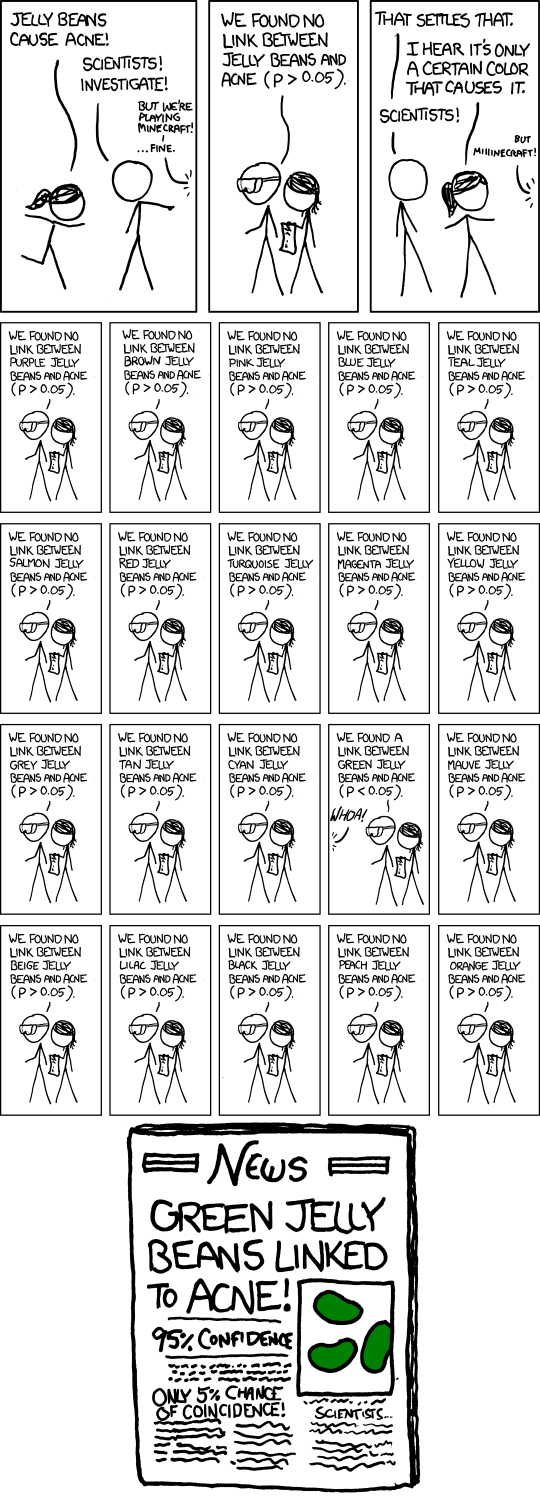
\includegraphics[width=0.4\linewidth]{img/significant} 

}

\caption{Dessin humoristique illustrant la problématique des tests multiples, par \href{https://xkcd.com/882}{XKCD}.}\label{fig:xkcd}
\end{figure}
\hypertarget{uxe9valuation-des-performances}{%
\subsection{Évaluation des performances}\label{uxe9valuation-des-performances}}

Lorsqu'une série de tests est réalisée et que la vérité est connue, il est possible de comparer le résultat avec l'attendu et de compter les effectifs dans les quatre configurations possibles.

Lorsqu'un test rejette l'hypothèse nulle à raison, on parlera de vrai positif et s'il la rejette à tort, il s'agira d'un faux positif. Si un test ne parvient pas à rejeter l'hypothèse nulle alors que celle-ci est vraie, il s'agit d'un vrai négatif alors que s'il aurait dû la rejeter, il s'agit d'un faux négatif.
Sur l'ensemble des tests, le nombre de vrais positifs, vrais négatifs, faux positifs et faux négatifs sont notés respectivement TP, TN, FP et FN. Ces quantités sont agrégées dans la \emph{matrice de confusion}, présentée dans la figure \ref{fig:conf}.


\begin{figure}

{\centering 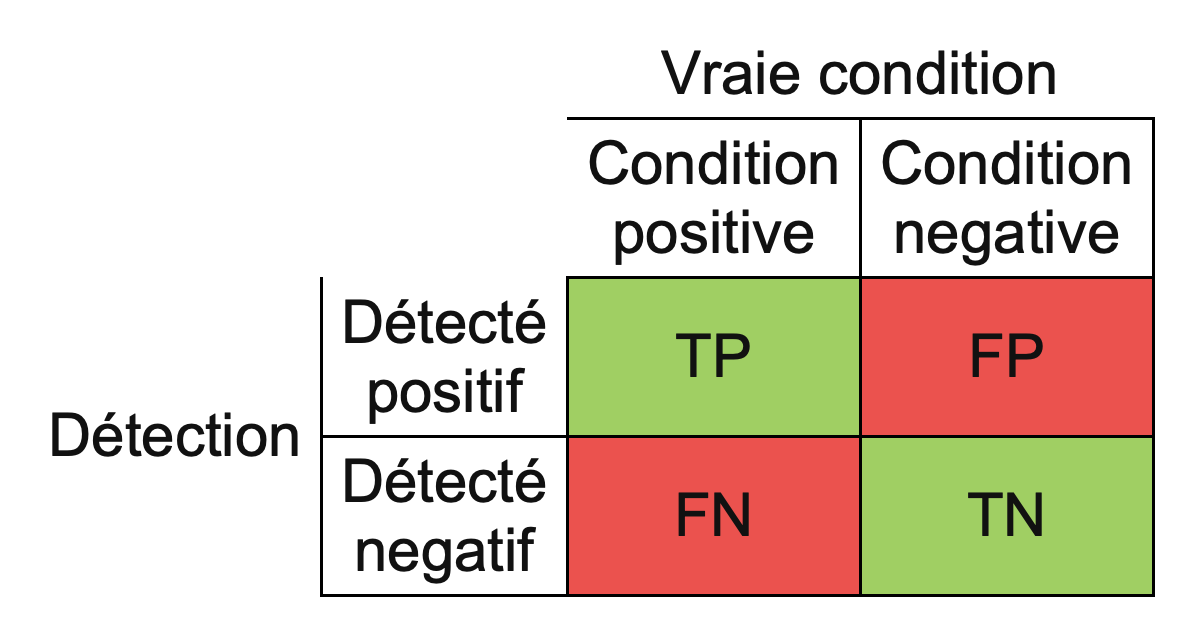
\includegraphics[width=0.7\linewidth]{img/confusionmatrix} 

}

\caption{Matrice de confusion. TP est le nombre de vrais positifs, TN le nombre de vrais négatifs, FP le nombre de faux positifs et FN le nombre de faux négatifs.}\label{fig:conf}
\end{figure}
À partir de ces mesures primaires, on peut définir le taux de vrais positifs (\emph{true positive rate}), appelé également puissance, sensibilité ou rappel :
\begin{equation*}
\text{TPR} = \frac{\text{TP}}{\text{TP} + \text{FN}},
\end{equation*}
qui représente la proportion d'espèces vraiment différentiellement abondantes que la méthode arrive à détecter. C'est une quantité que l'on souhaite maximiser. Cependant, un test qui détecterait toutes les espèces comme différentiellement abondantes aurait un TPR au maximum, à \(1\). Il faut donc aussi pouvoir contrôler que l'on ne rejette pas trop à tort, en contrôlant soit directement le nombre de faux positifs FP, soit la proportion de faux positifs parmi les positifs (\emph{false discovery proportion}) :
\begin{equation*}
\text{FDP} = \frac{\text{FP}}{\text{TP} + \text{FP}}.
\end{equation*}
\newline

Le FDP est lié à la précision \(\text{PPV}\) (\emph{positive predictive value}) via \(\text{PPV} = 1 - \text{FDP}\). Celle-ci mesure la crédence que l'on peut accorder au test sachant qu'il a rejeté l'hypothèse nulle.

Une fois que l'on maximise la puissance d'un test tout en contrôlant le nombre ou la proportion de fausses découvertes, il est intéressant d'avoir des métriques qui combinent ces métriques secondaires, comme l'exactitude (\emph{accuracy}), qui est la proportion de fois où le test a correctement assigné les bactéries :
\begin{equation*}
\text{ACC} =\frac{\text{TP} + \text{TN}}{\text{TP} + \text{FP} + \text{FN} + \text{TN}},
\end{equation*}
ou du score \(\text{F}_1\) qui est la moyenne harmonique entre la précision et le rappel :
\begin{equation*}
\text{F}_1 = \frac{2}{\frac{1}{\text{TPR}} + \frac{1}{\text{PPV}}} = \frac{2 \text{TP}}{2\text{TP} + \text{FP} + \text{FN}}.
\end{equation*}
Ces deux quantités sont à valeurs dans \(\mathopen[0,1\mathclose]\) et plus elles sont proches de \(1\), plus le modèle est performant.

Les mesures présentées auparavant sont valables quelque soit le seuil à partir duquel on rejette l'hypothèse nulle, couramment égal à \(0.05\). Il peut alors être intéressant de regarder ces quantités comme une fonction du seuil de rejet \(t\) : \(\text{TPR}(t)\), \(\text{FDP}(t)\), \(\text{ACC}(t)\)\ldots{}

On définit alors la courbe ROC (\emph{receiver operating characteristic}) comme étant la sensibilité en fonction de la spécificité pour les différents seuils, soit l'ensemble des points \(\left(\text{FDP}(t), \text{TPR}(t)\right)_{t\in\mathopen[0,1\mathclose]}\).

Lorsque \(t=0\), on ne rejette jamais, il n'y a ni faux positif ni vrai positif et on est en \((0,0)\). Lorsque \(t=1\), on rejette tout le temps, \(\text{FN} = \text{TN} = 0\) et on est en \((1,1)\). \(\text{FDP}\) et \(\text{TPR}\) sont des fonctions croissantes en \(t\). En \((0,1)\), il n'y a ni faux négatif ni faux positif et le test est toujours correct. La courbe ROC relie donc \((0,0)\) à \((1,1)\) et plus elle s'approche de \((0,1)\), mieux c'est. L'aire sous la courbe ROC, dite AUC pour \emph{area under the curve}, permet de quantifier la qualité d'un classificateur indépendamment du seuil choisi. Plus l'AUC est proche de \(1\), plus le classificateur est performant.

\hypertarget{correction-de-bonferroni}{%
\subsection{Correction de Bonferroni}\label{correction-de-bonferroni}}

La correction de Bonferroni a pour objectif de contrôler le \emph{family-wise error rate}, la probabilité de faire au moins une erreur dans les découvertes en changeant le seuil auquel on rejette l'hypothèse nulle. Si au lieu de rejeter en dessous du seuil \(\alpha\), on rejette en dessous de \(\frac{\alpha}{m}\), on contrôle le FWER au niveau \(\alpha\) :
\begin{align*}
\text{FWER} & = \PP{\text{FP} \geq 1} \\
& = \PP{\bigcup_{i\in \mathbb{H}_0} \left\{\pv_i \leq \frac{\alpha}{m}\right\} } \\
& \leq \sum_{i\in \mathbb{H}_0} \PP{\left\{\pv_i \leq \frac{\alpha}{m} \right\}} \\
& = m_0 \frac{\alpha}{m}  \\
& \leq \alpha.
\end{align*}
Pour plus de praticité, on travaille avec les \(q\)-valeurs --ou \(p\)-valeurs ajustées-- associées à la correction de Bonferroni définies par
\begin{equation*}
\qv^{\text{bonf}} = m * \pv,
\end{equation*}
qui sont, elles, comparées au seuil \(\alpha\).

Ainsi, avec une probabilité de \(1-\alpha\), il n'y a aucun faux positif pour l'ensemble des tests réalisés.

Cependant, les procédures qui contrôlent le FWER comme les corrections de Bonferroni ou de Holm, une alternative plus puissante (Holm, \protect\hyperlink{ref-holm1979simple}{1979}), sont très conservatrices et peu utilisées en métagénomique.

\hypertarget{correction-de-benjamini-hochberg}{%
\subsection{Correction de Benjamini-Hochberg}\label{correction-de-benjamini-hochberg}}

Au lieu de n'autoriser aucun faux positif à un risque \(\alpha\), Benjamini \& Hochberg (\protect\hyperlink{ref-benjamini1995controlling}{1995}) proposent de contrôler la proportion de fausses découvertes parmi les découvertes. Il s'agit alors de garder la quantité \(\text{FDP} = \frac{\text{FP}}{\text{R} \vee 1}\) en dessous d'un seuil \(\alpha\), où \(\text{R} = \text{TP} + \text{FP}\) est le nombre d'hypothèses rejetées.

Sous réserve d'une indépendance entre les tests, la procédure de Benjamini-Hochberg (BH) contrôle l'espérance du \(\text{FDP}\), appelée FDR (pour \emph{false discovery rate}), au seuil \(\alpha\). Celle-ci se fait en trois étapes :
\begin{itemize}
\item
  ordonner les \(p\)-valeurs \(\pv_{(1)}, \ldots, \pv_{(m)}\) et poser \(\pv_{(0)} = 0\) ;
\item
  trouver le rang \(\hat{\ell} = \max\left\{\ell \in [\![0,m]\!] \left| \pv_{(\ell)} \leq \frac{\alpha\ell}{m} \right. \right\}\) ;
\item
  rejeter les \(\hat{\ell}\) hypothèses correspondant aux plus petites \(p\)-valeurs.
\end{itemize}
En effet, notons \(V_i = \indic_{\left\{H_i \text{ est rejetée}\right\}}\) pour \(i \in \mathbb{H}_0\). On a alors
\(\text{FDP} = \frac{\text{FP}}{\text{R} \vee 1} = \sum_{i\in \mathbb{H}_0} \frac{V_i}{\text{R} \vee 1}\).

Fixons \(i\in \mathbb{H}_0 \neq \emptyset\). S'il y a \(k\) hypothèses rejetées, alors \(H_i\) est rejetée si et seulement si \(\pv_i \leq \frac{\alpha k}{m}\) et alors \(V_i = \indic_{\left\{\pv_i \leq \frac{\alpha k}{m}\right\}}\). Définissons \(\text{R}(\pv_i \rightarrow 0)\) le nombre d'hypothèses rejetées lorsqu'on fixe \(\pv_i\) à \(0\). S'il y a \(k\) hypothèses rejetées et que \(\pv_i \leq \frac{\alpha k}{m}\), \(H_i\) est rejetée et fixer \(\pv_i\) à \(0\) ne change pas le nombre d'hypothèses rejetées : \(\text{R} = \text{R}(\pv_i \rightarrow 0)\). À l'inverse, si \(\pv_i > \frac{\alpha k}{m}\), \(H_i\) n'est pas rejetée et \(V_i = 0\). La concaténation des deux résultats précédents donne \(V_i\indic_{\left\{\text{R}=k\right\}} = V_i\indic_{\left\{\text{R}(\pv_i \rightarrow 0) = k\right\}}\).

En notant \(\mathcal{F}_i = \sigma\left(\left\{\pv_1, \ldots, \pv_{i-1}, \pv_{i+1}, \ldots, \pv_m \right\}\right)\) la tribu engendrée par les \(p\)-valeurs sauf \(\pv_i\),
\begin{equation*}
\begin{aligned}
\EE{\left.\frac{V_i}{\text{R}\vee 1} \right| \mathcal{F}_i} & = \EE{\left.\sum_{k = 1}^m\frac{V_i\indic_{\left\{\text{R}=k\right\}}}{k} + \frac{0}{0\vee1} \right| \mathcal{F}_i} \\
& = \sum_{k = 1}^m \EE{\left.\frac{V_i\indic_{\left\{\text{R}(\pv_i \rightarrow 0)=k\right\}}}{k}\right| \mathcal{F}_i} \\
& = \sum_{k = 1}^m \indic_{\left\{\text{R}(\pv_i \rightarrow 0)=k\right\}} \EE{\left.\frac{\indic_{\left\{\pv_i \leq \frac{\alpha k}{m}\right\}}}{k}\right| \mathcal{F}_i} \\
& = \sum_{k = 1}^m \indic_{\left\{\text{R}(\pv_i \rightarrow 0)=k\right\}} \frac{\alpha}{m} \\
& = \frac{\alpha}{m}.
\end{aligned}
\end{equation*}
La troisième égalité provient du fait que \(\text{R}(\pv_i \rightarrow 0)\) est connue conditionnellement à \(\mathcal{F}_i\), la quatrième découle du fait que \(\pv_i \sim \unif{\mathopen[0, 1\mathclose]}\) et la dernière résulte du fait qu'en fixant une \(p\)-valeur à \(0\), on va rejeter au moins une fois et \(\text{R}(\pv_i \rightarrow 0)\) est compris entre \(1\) et \(m\).

Finalement,
\begin{equation*}
\text{FDR} = \EE{\text{FDP}} = \EE{\sum_{i\in \mathbb{H}_0} \frac{V_i}{\text{R} \vee 1}} = \sum_{i\in \mathbb{H}_0}\frac{\alpha}{m} \leq \alpha.
\end{equation*}
En terme de \(q\)-valeurs,
\begin{equation*}
\qv^{\text{bh}}_{(i)} = \min\left\{\min_{j\ge i}\left\{\frac{m\pv_{(j)}}{j}\right\},1\right\},
\end{equation*}
où \(\pv_{(1)}, \ldots, \pv_{(m)}\) sont les \(p\)-valeurs réordonnées et \(\qv^{\text{bh}}_{(i)}\) est la \(q\)-valeur associée à \(\pv_{(i)}\).

\hypertarget{correction-de-benjamini-yekutieli}{%
\subsection{Correction de Benjamini-Yekutieli}\label{correction-de-benjamini-yekutieli}}

Si les tests ne sont pas indépendants, il est possible d'appliquer la procédure de Benjamini-Yekutieli (BY) (Benjamini \& Yekutieli, \protect\hyperlink{ref-benjamini2001control}{2001}) qui ne requiert aucune hypothèse d'indépendance entre les tests. Il s'agit d'une modification dans la procédure de Benjamini-Hochberg, où l'on ne compare plus à \(\frac{\alpha\ell}{m}\) mais à \(\frac{\alpha\ell}{m\sum_{i = 1}^m \frac{1}{\ell}}\).

Les \(q\)-valeurs sont alors
\begin{equation*}
\qv^{\text{by}}_{(i)} = \min\left\{\min_{j\ge i}\left\{\sum_{i = 1}^m \frac{1}{i} \frac{ m\pv_{(j)}}{j}\right\},1\right\}.
\end{equation*}
Cette procédure très générique présente l'inconvénient d'être extrêmement conservatrice et de faire peu de découvertes.

\hypertarget{procuxe9dures-hiuxe9rarchiques-pour-tests-multiples}{%
\section{Procédures hiérarchiques pour tests multiples}\label{procuxe9dures-hiuxe9rarchiques-pour-tests-multiples}}

Jusqu'alors, les corrections proposées font l'hypothèse (\emph{a priori} fausse) que les tests sont indépendants ou vérifient une hypothèse technique de dépendance positive, comme BH, ou fonctionnent quelque soit la relation de dépendance entre les tests, au prix d'un fort conservatisme, comme BY.

Il serait plus intéressant d'utiliser explicitement la relation de dépendance entre les tests afin d'augmenter la puissance statistique. C'est ce que proposent les méthodes présentées dans cette section.

Cette section ne nécessite qu'une définition intuitive de ce qu'est un arbre : un graphe acyclique connexe orienté dont les nœuds terminaux (feuilles) sont étiquetés et ayant ou non des longueurs de branches. Une définition plus rigoureuse en sera donnée dans le chapitre \ref{arbres}.

\hypertarget{treefdr}{%
\subsection{\texorpdfstring{\emph{TreeFDR}}{TreeFDR}}\label{treefdr}}

\emph{TreeFDR} (Xiao, Cao, \& Chen, \protect\hyperlink{ref-xiao2017false}{2017}) est une procédure de lissage des \(z\)-scores suivie d'une procédure de correction par permutation implémentée dans le package \texttt{\{StructFDR\}}.

Dans ce modèle hiérarchique, les \(z\)-scores \(\zs = \Phi^{-1}\left(\pv\right)\) sont vus comme la réalisation d'un vecteur gaussien multivarié de moyenne \(\mu\) :
\begin{equation*}
\left. \zs \mid \mu \right. \sim \mathcal{N}_m\left(\mu,\sigma^2 \mathbf{I}_m\right).
\end{equation*}
À partir de l'arbre, on calcule la matrice des distances patristiques entre feuilles \(D = (d_{i,j})_{i,j}\) que l'on converti en une matrice de corrélation \(C_{\rho} = \left(\exp\left(-2\rho D_{i,j}\right)\right)_{i,j}\). Cette matrice de corrélation est ensuite utilisée pour décrire les corrélations entre les composantes de \(\mu\) :
\begin{equation*}
\mu \sim \mathcal{N}_m\left(\gamma \mathbf{1}_m,\tau^2C_{\rho}\right).
\end{equation*}
L'estimateur du maximum \emph{a posteriori} de \(\mu\) est alors
\begin{equation*}
\mu^* = \left(\mathbf{I}_m + k^2 C_{\rho}^{-1}\right)\left(k^2 C_{\rho}^{-1} \gamma \mathbf{1}_m + \zs \right),
\end{equation*}
avec \(k = \frac{\sigma}{\tau}\).

Les hyperparamètres \(\rho\) et \(k\) contrôlent le niveau de lissage du modèle : les \(z\)-scores issus d'un même clade vont être regroupés vers une valeur commune. De hautes valeurs de \(k\) ou de faibles valeurs de \(\rho\) entraînent un fort lissage.

\hypertarget{fdr-hiuxe9rarchique}{%
\subsection{FDR hiérarchique}\label{fdr-hiuxe9rarchique}}

Le FDR hiérarchique (hFDR) est une procédure proposée par Yekutieli (\protect\hyperlink{ref-yekutieli2008hierarchical}{2008}) et implémentée dans le \emph{package} R \texttt{\{structSSI\}} (Sankaran \& Holmes, \protect\hyperlink{ref-sankaran2014structssi}{2014}).

Contrairement à \emph{TreeFDR}, le FDR hiérarchique a besoin d'avoir une \(p\)-valeur à chaque nœud interne. Dans le cas de données métagénomiques, celles-ci peuvent facilement être obtenues en effectuant un test d'abondance différentielle sur la somme des bactéries qui descendent du nœud considéré.

C'est un algorithme descendant qui teste les hypothèses par \emph{familles} --c'est à dire tous les enfants d'un même nœud-- au niveau \(\alpha\) en corrigeant avec BH à chaque fois. Plus précisément, on commence par tester la famille de la racine (avec une correction de BH). Puis, pour chaque nœud rejeté au sein de cette famille, on va tester ses enfants (en corrigeant toujours avec BH). À l'inverse, si un nœud n'est pas rejeté, aucun de ses enfants directs et de ses descendants n'est testé. L'algorithme se termine une fois arrivé aux feuilles ou lorsqu'il ne reste que des nœuds qui n'ont pas pu être rejetés. La figure \ref{fig:hfdr} illustre cette procédure sur un arbre à \(6\) feuilles.


\begin{figure}

{\centering 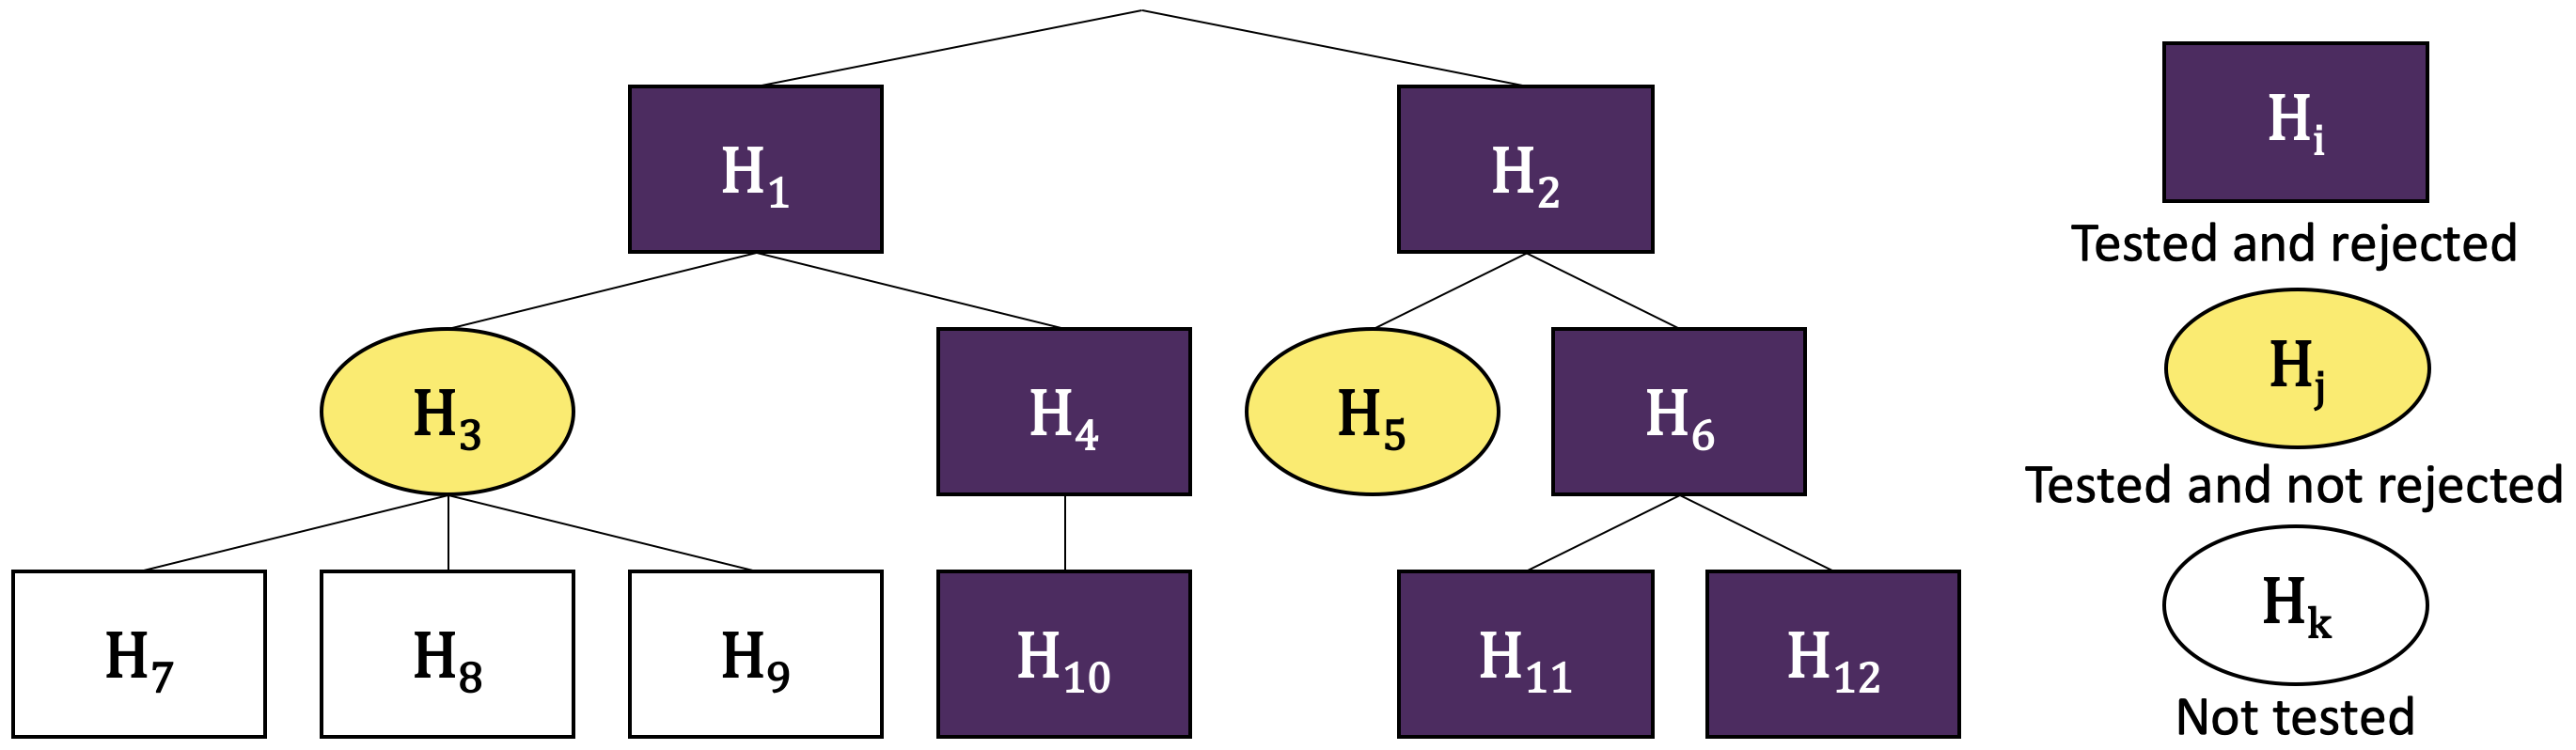
\includegraphics[width=0.9\linewidth]{img/hfdr} 

}

\caption{Exemple d'une procédure de FDR hiérarchique. Les hypothèses à tester sont notées \(H_1\) à \(H_{12}\). L'algorithme commence par tester et rejeter (après correction) \(H_1\) et \(H_2\). Puis il teste la famille \((H_3, H_4)\), car ce sont des enfants de \(H_1\), et rejette \(H_4\) mais pas \(H_3\). La famille \((H_7, H_8, H_9)\) n'est pas testée car \(H_3\) n'a pas été rejeté. \(H_{10}\) est testé et rejeté. L'algorithme procède de même sur les descendants de \(H_2\). En définitive, il y a trois découvertes aux feuilles (\(H_{10}\), \(H_{11}\) et \(H_{12}\)) pour \(5\) familles testées. Le FDR a \emph{posteriori} pour les feuilles est alors de \(1.44 \times \alpha \times 2\).}\label{fig:hfdr}
\end{figure}
Alors que \(\alpha\) est le niveau de contrôle \emph{a priori} intra-familles, si l'on ne considère que les découvertes au niveau des feuilles, hFDR garantit un contrôle \emph{a posteriori} au niveau
\begin{equation*}
\alpha' = 1.44 \times \alpha \times \frac{\# \text{découvertes} + \#\text{familles testées}}{\# \text{découvertes} + 1}.
\end{equation*}
\newline

Cette méthode souffre de plusieurs problèmes majeurs. Tout d'abord, le contrôle du FDR est fait seulement \emph{a posteriori}, et plusieurs essais sont nécessaires pour contrôler le FDR au niveau souhaité, sans avoir la certitude que cela soit possible.
De plus, pour que la procédure descende jusqu'aux feuilles, il faut que le signal d'abondance différentielle soit détectable dès la famille de la racine, sinon la procédure s'arrête dès le début, et cela arrive souvent en pratique (Huang et al., \protect\hyperlink{ref-huang2020treeclimbr}{2020}).

Enfin, dans son implémentation par Sankaran \& Holmes (\protect\hyperlink{ref-sankaran2014structssi}{2014}), les \(p\)-valeurs d'entrées ne sont pas données en argument par l'utilisateur mais calculées au sein la procédure via une ANOVA à un facteur. Ce type de test n'est malheureusement pas adapté aux données métagénomiques, ce qui fait perdre de la puissance à la procédure (Bichat, Plassais, Ambroise, \& Mariadassou, \protect\hyperlink{ref-bichat2020incorporating}{2020}). Pour ces raisons, la procédure hFDR ne sera pas comparée aux autres méthodes dans la section \ref{nouvelleapproche}.

\hypertarget{treeclimbr}{%
\subsection{\texorpdfstring{\emph{treeclimbR}}{treeclimbR}}\label{treeclimbr}}

Huang et al. (\protect\hyperlink{ref-huang2020treeclimbr}{2020}) ont récemment proposé \emph{treeclimbR}, une procédure ascendante qui permet de sélectionner directement des clades différentiellement abondants.

Tout d'abord, pour chaque nœud interne, on agrège les abondances en les sommant sur ses descendants. Puis, pour chaque nœud \(i\) (interne ou feuille), on effectue un test qui renvoie une \(p\)-valeur \(\pv_i\) ainsi que le signe \(\sign_i\in \{-1,1\}\) associé à la direction du changement d'abondance.

On calcule ensuite un score à chaque nœud défini par
\begin{equation*}
U_i(t) = \left|\frac{\sum_{k \in \desc(i)} \sign_k \indic_{\{\pv_i < t\}}}{\#\desc(i)}\right|
\end{equation*}
où \(t \in \mathopen[0,1\mathclose]\) est un hyperparamètre que l'on va estimer dans la suite et \(\desc(i)\) est l'ensemble des descendants de \(i\). Lorsque \(U_i(t)\) est proche de \(1\), cela signifie que les descendants de \(i\) sont différentiellement abondants et dans le même sens. À l'inverse, quand \(U_i(t)\) s'approche de \(0\), soit les espèces ne sont pas différentiellement abondantes, soit elles le sont dans des directions opposées.

Pour chaque \(t\) candidat sur une grille, on parcours l'arbre depuis la racine et on arrête la descente d'une branche lorsque l'on rencontre un nœud \(i\) tel que \(U_i(t) = 1\) : il s'agit d'un nœud terminal pour la procédure, qui représente tous ses descendants.

On effectue ensuite une correction pour test multiple (Benjamini-Hochberg) sur les nœuds terminaux et les feuilles qui ne font pas partie de la descendance d'un nœud terminal.

Il reste à sélectionner le meilleur \(t\) candidat. On utilise trois critères éliminatoires. Le premier est un choix \emph{a posteriori} d'une borne maximale \(t_{\max}\) pour \(t\) (dépendante des résultats) et on exclut les candidats tels que \(t\in\mathopen[0, t_{\max}\mathclose]\), ceci permettant de contrôler le FDR au niveau des feuilles parmi les candidats restants. Puis on ne conserve que les candidats ayant le plus grand nombre de feuilles rejetées, ce qui maximise la puissance. Et enfin, parmi les candidats restants, on ne garde que ceux qui minimisent le nombre de nœuds rejetés, pour retenir le niveau de résolution le plus adapté.

\hypertarget{arbres}{%
\chapter{Arbres}\label{arbres}}

\hypertarget{duxe9finitions}{%
\section{Définitions}\label{duxe9finitions}}

Un arbre est un graphe connexe acyclique. Les nœuds de degré \(1\) sont appelés feuilles, par oppositions aux nœuds internes.

Un arbre enraciné est un graphe connexe acyclique dirigé possédant une unique racine. Chaque nœud \(i\), à l'exception de la racine, a un unique parent noté \(\pa(i)\). Les feuilles sont les nœuds n'ayant pas de fils. Il est possible d'enraciner un arbre non-raciné en choisissant un nœud quelconque et en orientant les arêtes de la racine vers les feuilles. La branche menant au nœud \(i\) est dénotée \(b_i\) et a pour longueur \(\ell_i\). On parle de topologie d'un arbre lorsqu'on fait abstraction de ses longueurs de branche.

On note \(\mrca(i,j)\) l'ancêtre commun le plus récent (\emph{most recent common ancestor}) aux nœuds \(i\) et \(j\) : \(\mrca(i,j) = \pa^k(i)\), soit le \(k\)-ième parent successif de \(i\), avec \(k = \argmin_{p\in \NN}\left\{\exists q \in \NN : \pa^p(i) = \pa^q(j)\right\}\), et \(\desc(i)\) les descendants de \(i\), soit l'ensemble des nœuds ayant \(i\) pour ancêtre, \(i\) inclus : \(\desc(i) = \left\{j : \exists k \in \NN : \pa^k(j)=i\right\}\).

Le nœud \(i\) est à distance \(t_i\) de la racine et on note \(t_{i,j} = t_{\mrca(i,j)}\).

La distance, dite patristique, entre les nœuds \(i\) et \(j\) est notée \(d_{i,j} = t_i + t_j - 2 t_{i,j}\).

\(\tilde{\ell}_{i,j} = t_i - t_{i,j}\) est la distance entre le nœud \(i\) et l'ancêtre commun le plus récent à \(i\) et \(j\).

Un arbre enraciné est \textbf{binaire} si tous ses nœuds internes ont exactement deux fils. En particulier, un arbre binaire à \(m\) feuilles possède \(n = 2m-2\) branches.

Un nœud est \textbf{polytomique} s'il a plus de deux fils.

Un arbre est \textbf{ultramétrique} s'il est raciné et si toutes les feuilles sont à la même distance de la racine.

Un \textbf{clade} est un sous-arbre, il contient un nœud et tous ses descendants.

Pour un arbre enraciné, la \textbf{matrice d'incidence} \(T = (t_{i,j}) \in\{0,1\}^{m \times n}\) encode les relations de descendance entre nœuds au sein de l'arbre. Pour une feuille \(i\) et un nœud quelconque \(j\), le coefficient \(t_{i,j}\) vaut \(1\) si \(i \in \desc(j)\). En particulier, la colonne \(t_j\) est l'indicatrice des feuilles issues du nœud \(j\) tandis que la ligne \(t_{i.}\) est l'indicatrice des ancêtres de la feuille \(i\).


\begin{figure}

{\centering 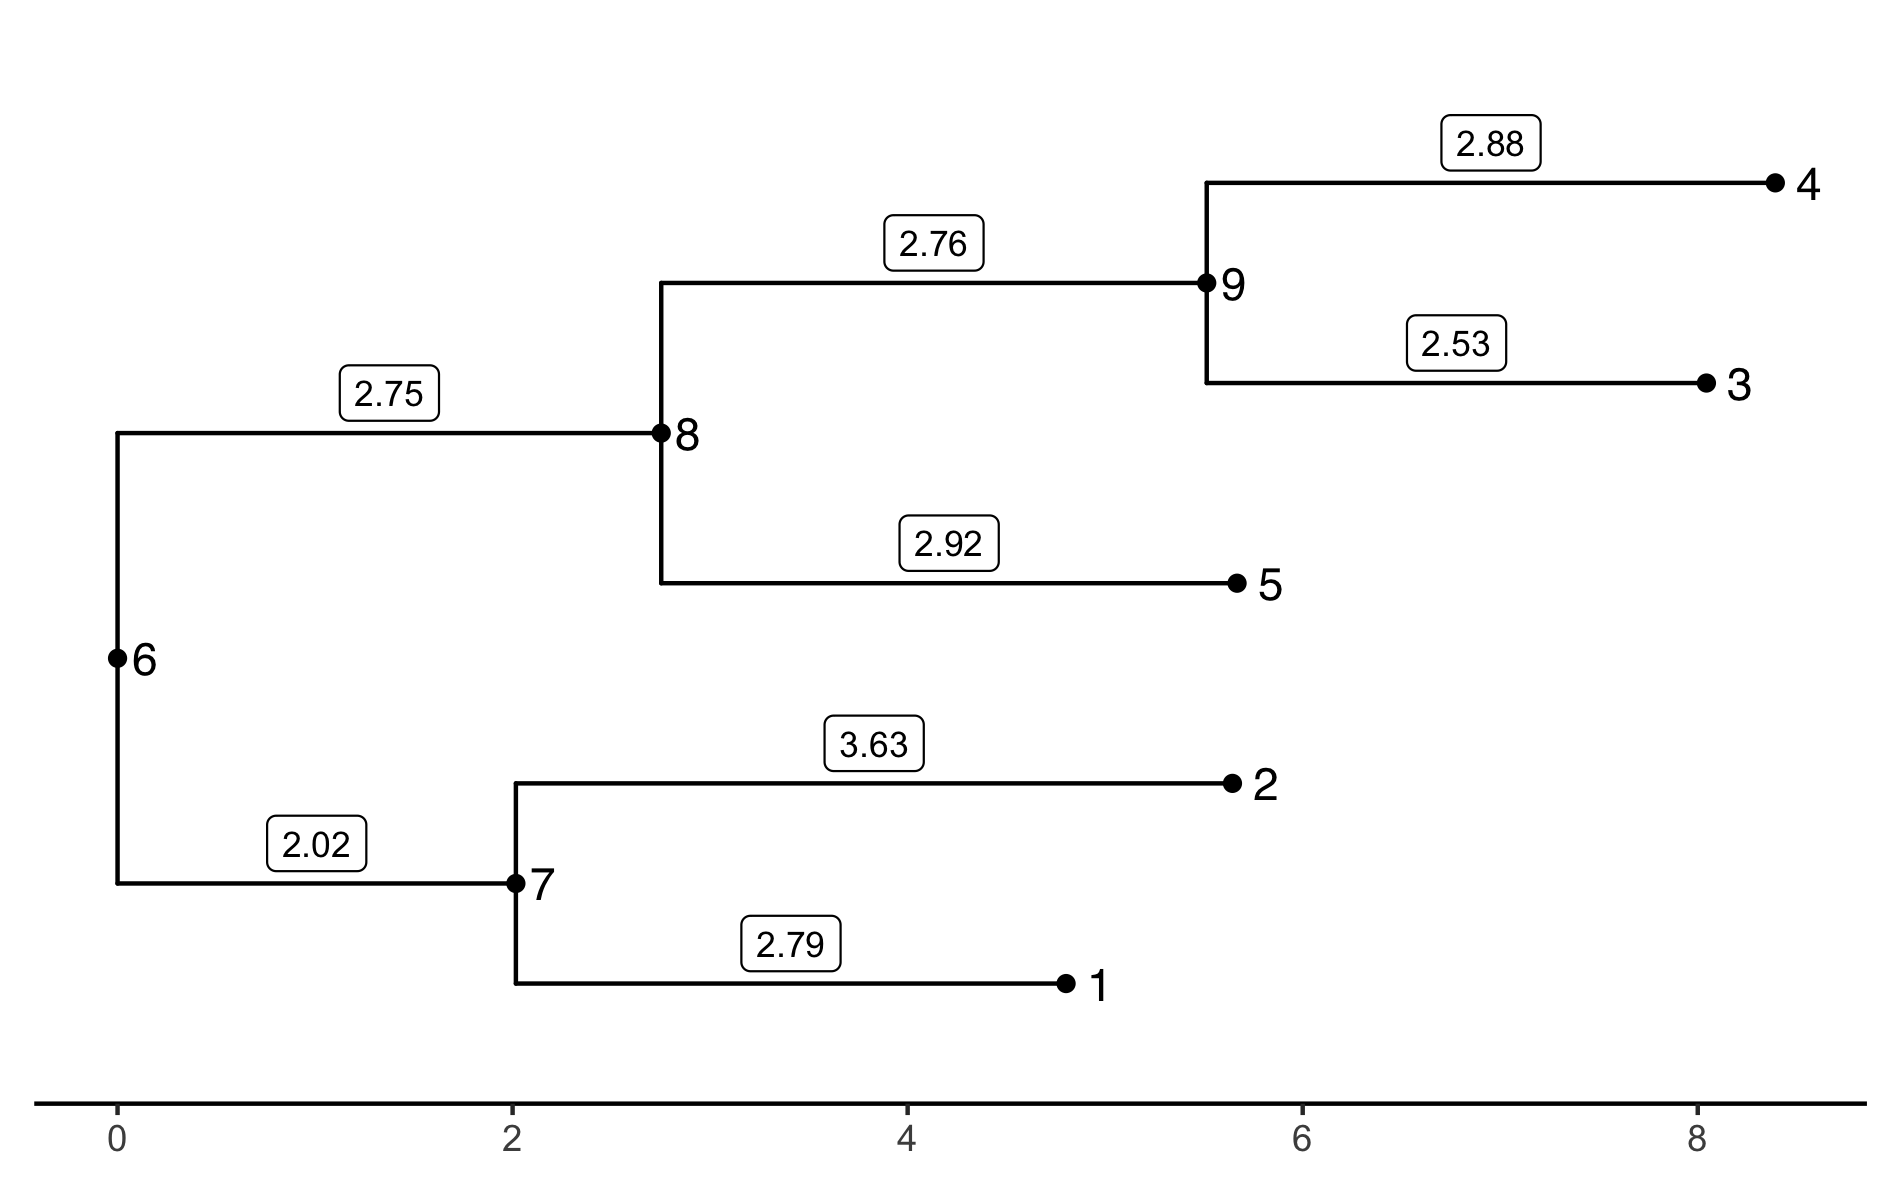
\includegraphics[width=0.9\linewidth]{img/tree_raw} 

}

\caption{Exemple d'un arbre enraciné binaire non ultramétrique à \(m = 5\) feuilles et \(n = 8\) branches.}\label{fig:treeraw}
\end{figure}
Illustrons les notations de cette section à l'aide de la figure \ref{fig:treeraw}. On a alors \(\pa(1) = \pa(2) = 7\), \(\desc(8) = \{3, 4, 5, 8, 9\}\), \(\mrca(5, 3) = 8\), \(\ell_1 = 2.79\), \(t_{3,4} = t_9 = \ell_8 + \ell_9 = 5.51\), \(t_{1,2} = t_7 = 2.02\), \(d_{3,5} = t_3 + t_5 - t_{3,5} = \ell_5 + \ell_9 + \ell_3 = 8.21\), \(\tilde{\ell}_{3,5} = t_3 - t_{3,5} = \ell_9 + \ell_3 = 5.29\) et
\begin{equation*}
T = 
\begin{bmatrix}
1 & 0 & 0 & 0 & 0 & 1 & 1 & 0 & 0 \\
0 & 1 & 0 & 0 & 0 & 1 & 1 & 0 & 0 \\
0 & 0 & 1 & 0 & 0 & 1 & 0 & 1 & 1 \\
0 & 0 & 0 & 1 & 0 & 1 & 0 & 1 & 1 \\
0 & 0 & 0 & 0 & 1 & 1 & 0 & 1 & 0 \\
\end{bmatrix}.
\end{equation*}
\hypertarget{distances}{%
\section{Distances}\label{distances}}

Les arbres sont des objets compliqués et plusieurs distances entre arbres ont été proposées dans la littérature. Nous en décrivons brièvement trois, qui mettent l'accent sur des aspects différents de l'arbre: topologie, longueurs de branche, combinaison des deux.

\hypertarget{distance-de-robinson-foulds}{%
\subsection{Distance de Robinson-Foulds}\label{distance-de-robinson-foulds}}

La distance de Robinson-Foulds (Robinson \& Foulds, \protect\hyperlink{ref-robinson1981comparison}{1981}) entre deux arbres racinés \(T\) et \(T'\) correspond intuitivement au nombre de branches spécifiques à un des deux arbres. Formellement, chaque nœud interne \(j\) définit une bipartition des feuilles et peut être associé à l'ensemble \(C_j \subset [\![1,m]\!]\) des feuilles issues du nœud \(j\). La colonne \(j\) de la matrice d'incidence précédemment introduite correspond en particulier à un codage binaire de \(C_j\). L'arbre \(T\) est ensuite recodé comme l'ensemble \(\mathcal{C}^T = \{C_j: j \in \text{nœud interne de } T\}\) de ses bipartitions. La distance de Robinson-Foulds entre \(T\) et \(T'\) est définie comme le cardinal de la différence symétrique entre \(\mathcal{C}^T\) et \(\mathcal{C}^{T'}\) :
\begin{equation*}
d(T, T') = | \mathcal{C}^T \setminus \mathcal{C}^{T'} | + | \mathcal{C}^{T'} \setminus \mathcal{C}^{T} |.
\end{equation*}
\hypertarget{distance-cophuxe9nuxe9tique}{%
\subsection{Distance cophénétique}\label{distance-cophuxe9nuxe9tique}}

La distance cophénétique entre deux arbres enracinés, introduite par Sokal \& Rohlf (\protect\hyperlink{ref-sokal1962comparison}{1962}), est basée sur les matrice des distances patristiques \(D^T = \left(d^T_{i,j}\right)_{i,j}\) entre paires de feuilles dans l'arbre \(T\), en particulier sur la vectorisation \(v^T\) de la partie triangulaire supérieure de \(D^T\), de longueur \(\frac{m(m-1)}{2}\). La distance cophénétique \(d(T, T')\) entre arbres \(T\) et \(T'\) est définie comme le complémentaire du coefficient de corrélation de Pearson entre \(v^{T_1}\) et \(v^{T_2}\):
\begin{equation*}
d(T, T') = 1 - \frac{ \frac{2\sum_{i < j} (d^{T}_{i,j} - \bar{d}^{T})(d^{T'}_{i,j} - \bar{d}^{T'})}{m(m-1)}}{\sqrt{\frac{2\sum_{i < j} (d^{T}_{i,j} - \bar{d}^{T})^2}{m(m-1)}} \sqrt{\frac{2\sum_{i < j} (d^{T'}_{i,j} - \bar{d}^{T'})^2}{m(m-1)}}} = 1 - \text{cor}(v^T, v^{T'})
\end{equation*}
où \(\bar{d}^{T} = \frac{2}{m(m-1)} \sum_{1 \leq i < j \leq m} d^{T}_{i,j}\). Cette distance ne prend en compte que la topologie de l'arbre.

\hypertarget{distance-de-billera-holmes-vogtmann-bhv}{%
\subsection{Distance de Billera-Holmes-Vogtmann (BHV)}\label{distance-de-billera-holmes-vogtmann-bhv}}

La distance BHV (Billera, Holmes, \& Vogtmann, \protect\hyperlink{ref-billera2001geometry}{2001}) est construite en plongeant l'espace \(\mathscr{T}_m\) des arbres à \(m\) feuilles dans \(\RR^m \times \RR^{2^{m}-m-1}\) puis en considérant la distance des plus courts chemins dans le sous-espace induit.

Formellement, un arbre binaire est définie par (i) sa topologie et (ii) ses longueurs de branches. Il existe \(m\) branches terminales (menant à une feuille) et \(2^{m} - m - 1\) branches internes distinctes, caractérisées chacune par l'ensemble des feuilles issues de cette feuille. Toutes ces branches ont une longueur positive. L'espace \(\mathscr{T}_m\) est donc naturellement plongé dans \(\RR_+^m \times \RR_+^{2^{m}-m-1}\). Le produit cartésien distingue les longueurs des branches externes (celles qui mènent aux feuilles, partagées par tous les arbres) de celles des branches internes, caractéristique d'une topologie donnée. Mais il n'en constitue qu'une sous-variété. En effet, à topologie \(T\) fixée, chaque longueur de branche peut varier dans \(\RR_+\). L'ensemble des arbres binaires de topologie \(T\), branches terminales omises, est donc identifiable à l'orthant ouvert \(\RR_+^{*, m-2}\). Si on fait tendre la longueur d'une branche interne vers \(0\), on se ramène à une topologie non-binaire \(\tilde{T}\), dans laquelle un unique nœud a exactement trois fils. Cette topologie peut également s'obtenir par contraction de branche interne à partir de deux autres topologies binaires \(T'\) et \(T''\). La topologie non-binaire \(\tilde{T}\) correspond à une \emph{frontière commune}, un sous-orthant de dimension \(m-3\) inclus dans chacun des trois orthants de dimension \(m-2\) caractérisant \(T\), \(T'\) et \(T''\). De façon générale, les sous-orthants de dimension \(m - 2 - k\) peuvent être identifiés à des topologies dégénérées, obtenues en contractant \(k\) branches internes d'un arbre binaire.

Il existe \((2m-3)!! = (2m-3)\times(2m-5)\times\dots\times5 \times 3 \times 1 = \prod_{i = 0}^{m-2} 2i+1\) topologies binaires (Cavalli-Sforza \& Edwards, \protect\hyperlink{ref-cavalli1967phylogenetic}{1967}) qui correspondent à autant d'orthants de dimension \(m-2\). \(\mathscr{T}_m\) est donc constitué de \((2m-3)!!\) orthants (un par topologie) de dimension \(m-2\), \emph{collés} entre eux par des sous-orthants de dimension inférieure et correspondant à des topologies non-binaires. La figure \ref{fig:bhvorthants} montre une jonction de tels orthants dans le cas où \(m=4\).


\begin{figure}

{\centering 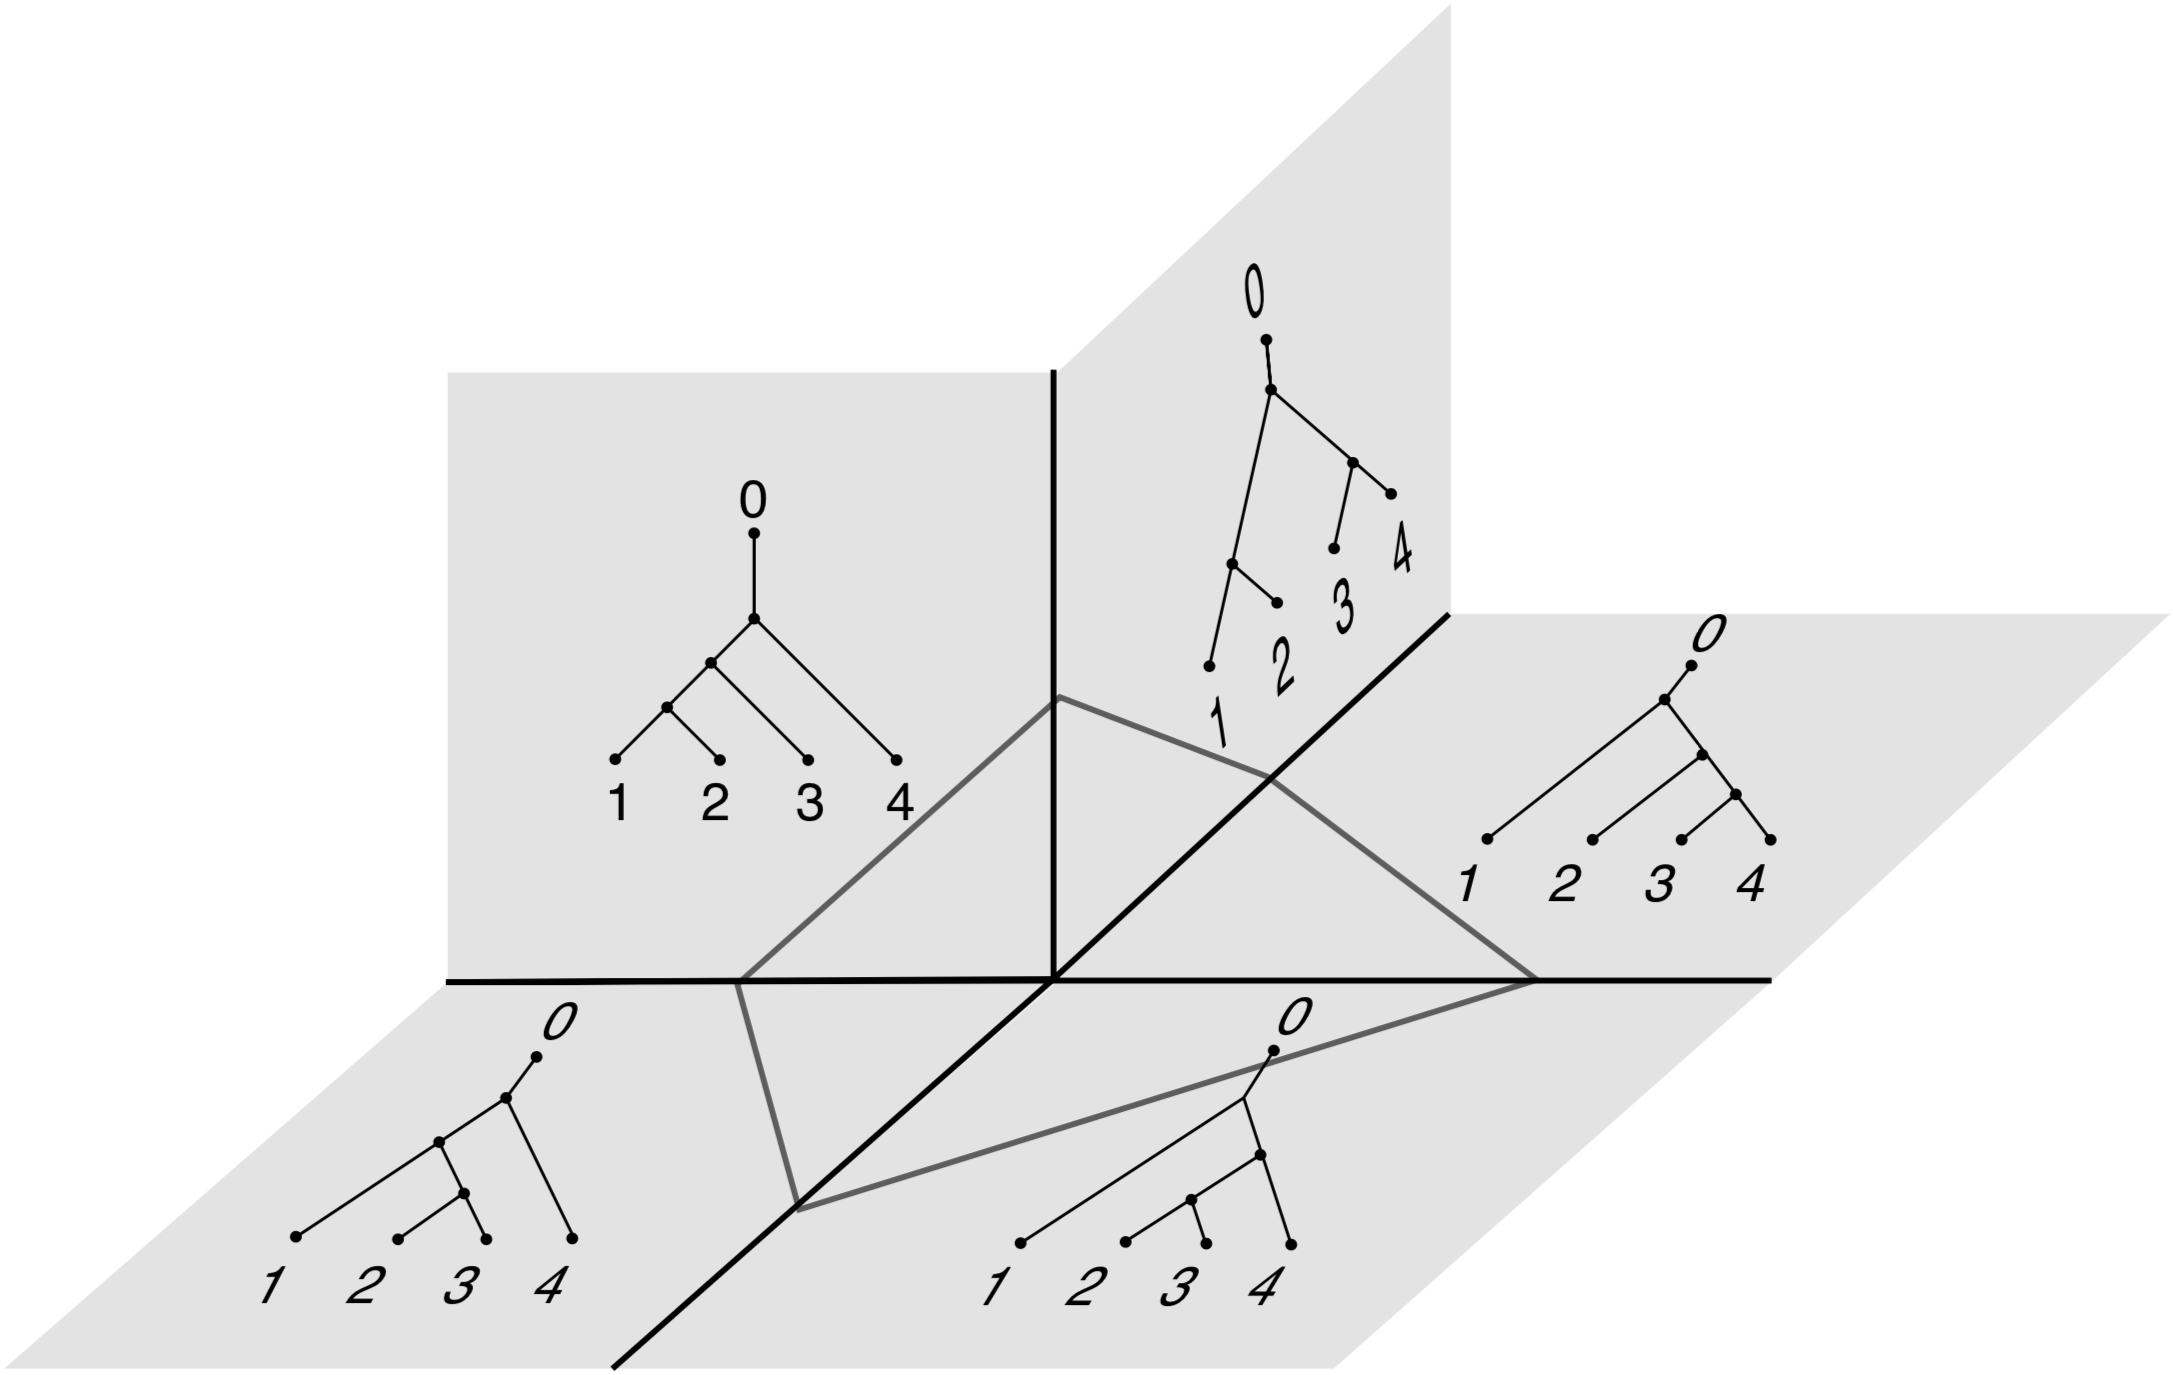
\includegraphics[width=0.9\linewidth]{img/bhv_orthants} 

}

\caption{Une partie de \(\mathscr{T}_4\), où cinq orthants se rejoignent, tiré de Billera et al. (\protect\hyperlink{ref-billera2001geometry}{2001}).}\label{fig:bhvorthants}
\end{figure}
Billera et al. (\protect\hyperlink{ref-billera2001geometry}{2001}) montrent que \(\mathscr{T}_m\) est connexe et possède une courbure négative. En particulier, pour toute paire d'arbres \(T\) et \(T'\), il existe un plus court chemin dans \(\mathscr{T}_m\) entre \(T\) et \(T'\). La distance BHV est la distance géodésique dans \(\mathscr{T}_m\), c'est à dire la distance du plus court chemin. Lorsque \(T\) et \(T'\) appartiennent au même orthant (c'est à dire partagent la même topologie), la distance géodésique coïncide avec la distance euclidienne dans l'orthant.

La figure \ref{fig:bhvdist} illustre un exemple plus complexe dans lequel le plus court chemin traverse plusieurs orthants. Dans cet exemple, la distance géodésique est la somme des distances euclidiennes du chemin parcouru dans chaque orthant. La distance BHV prend en compte la topologie, les longueurs de branche et la géométrie de \(\mathscr{T}_m\) mais son calcul effectif est nettement plus coûteux que celui des distances cophénétiques et de Robinson-Foulds (Owen \& Provan, \protect\hyperlink{ref-owen2010fast}{2010}).


\begin{figure}

{\centering 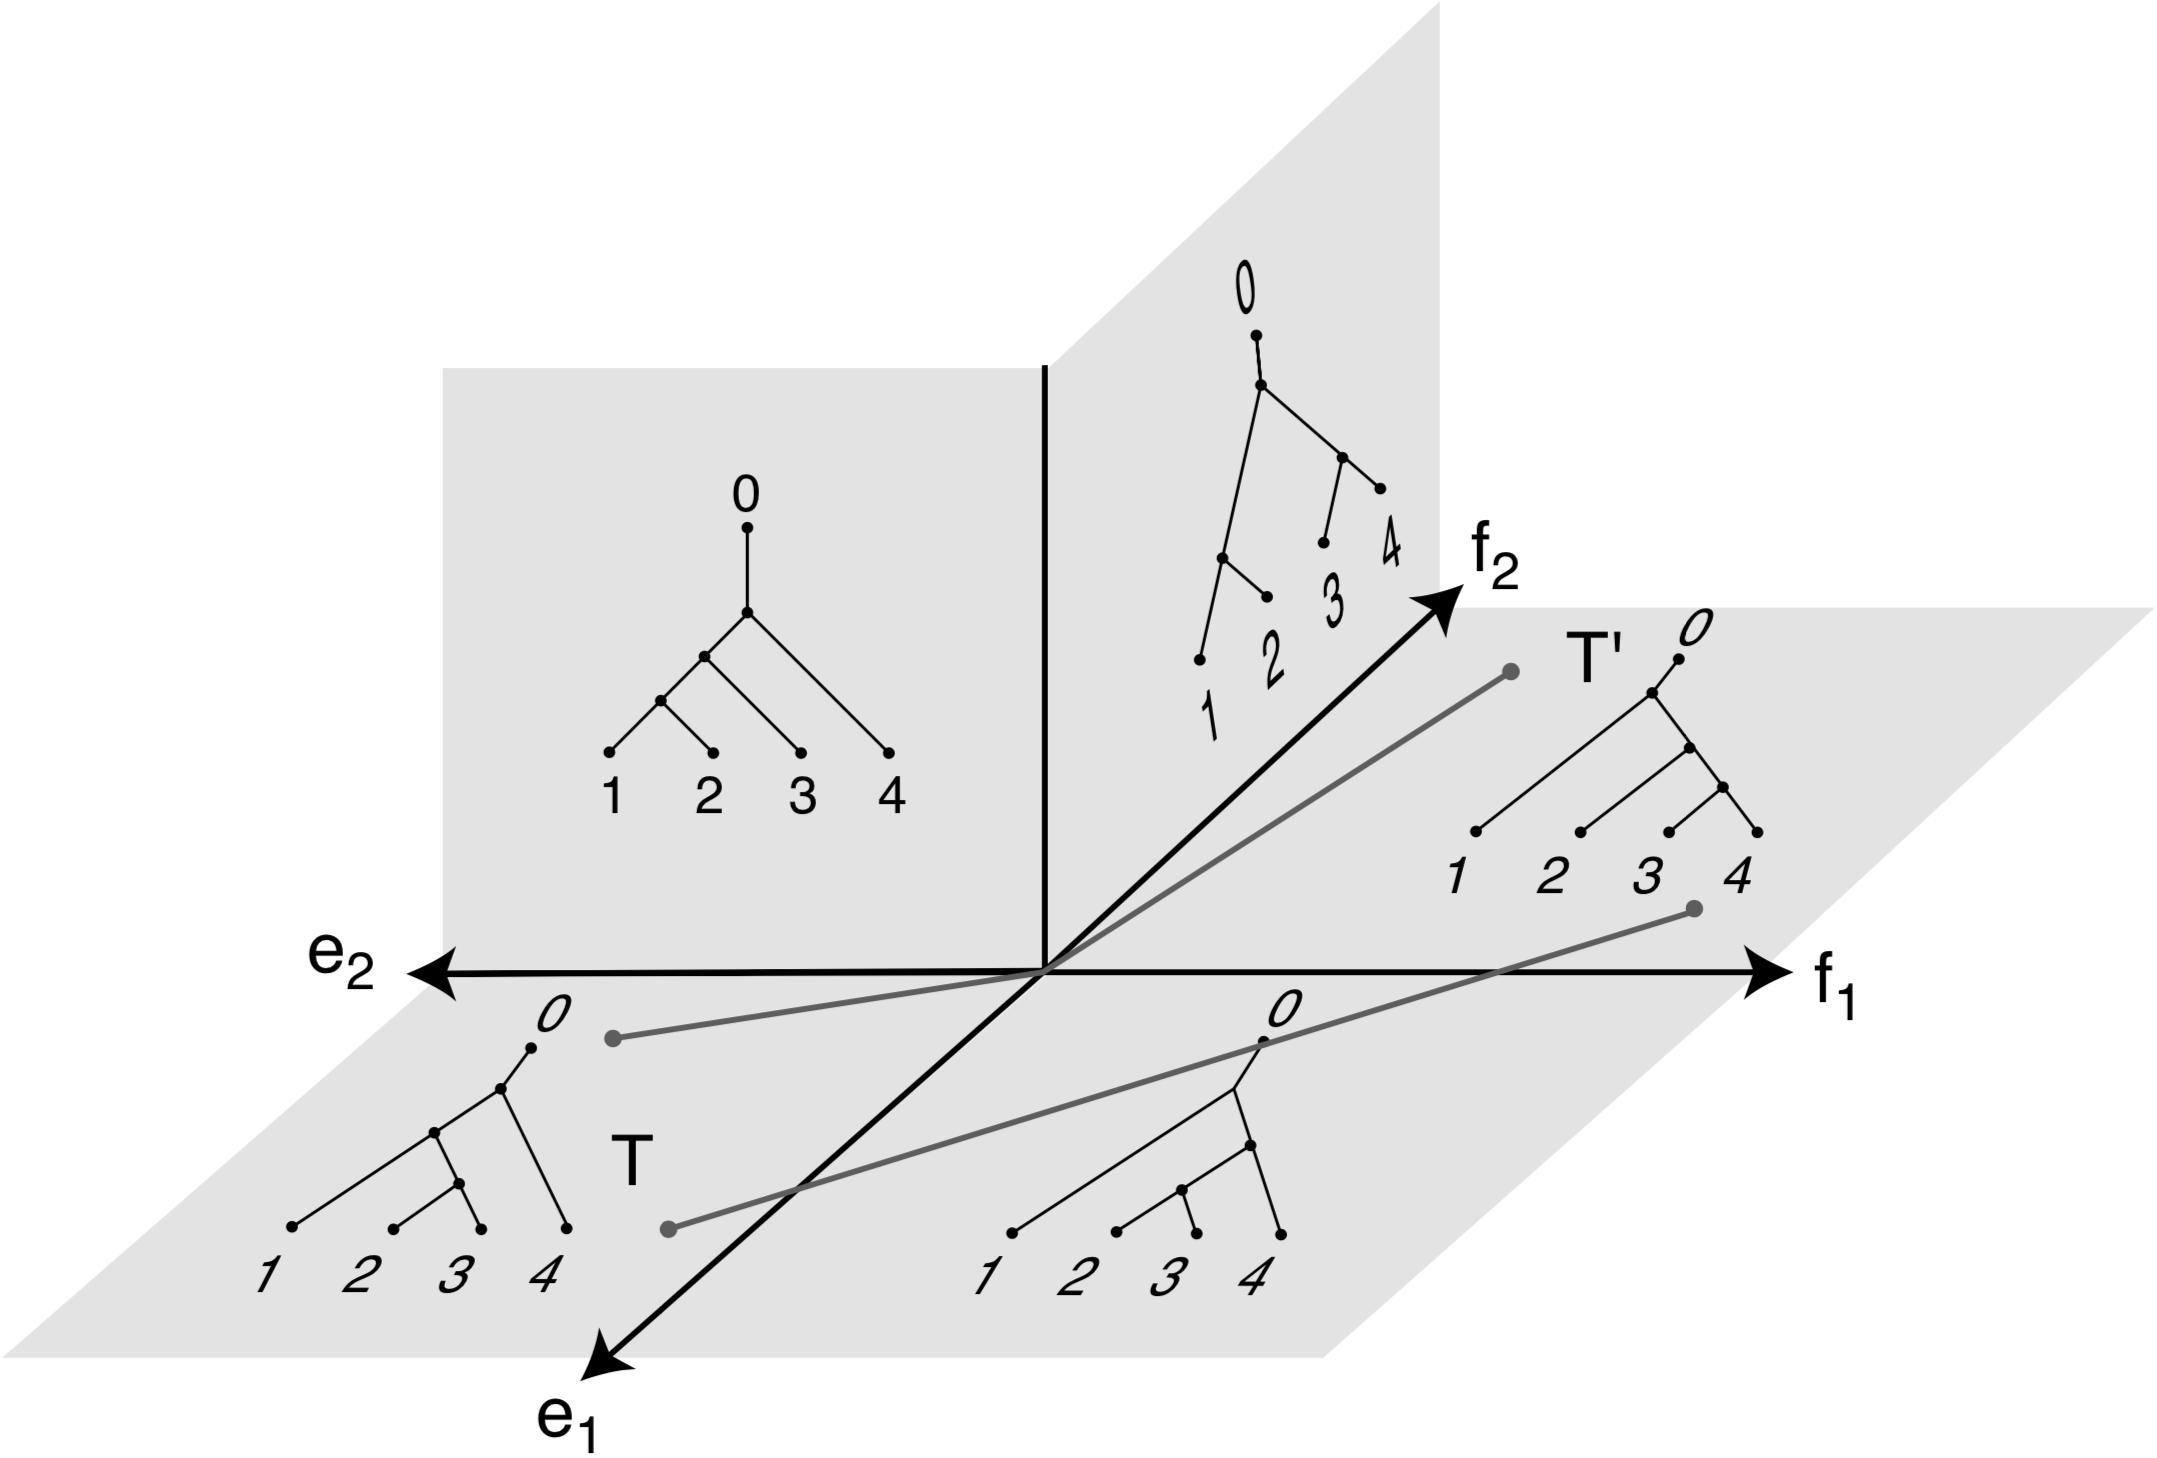
\includegraphics[width=0.9\linewidth]{img/bhv_dist} 

}

\caption{Des chemins traversant plusieurs orthants dans \(\mathscr{T}_4\), tiré de Billera et al. (\protect\hyperlink{ref-billera2001geometry}{2001}).}\label{fig:bhvdist}
\end{figure}
\hypertarget{arbres-dintuxe9ruxeat}{%
\section{Arbres d'intérêt}\label{arbres-dintuxe9ruxeat}}

Dans nos analyses, nous considérons trois types d'arbre : taxonomique, phylogénétique ou de corrélation. Les deux premiers représentent l'histoire évolutive des taxons et sont reconstruits à partir de données phénotypiques et moléculaires. Le dernier est reconstruit à partir des tableaux d'abondance et représente les similarités en terme de profils d'abondance.

\hypertarget{phyloguxe9nie}{%
\subsection{Phylogénie}\label{phyloguxe9nie}}

L'arbre phylogénétique, ou phylogénie, traduit les relations de parenté entre organismes. Pour un séquençage avec gène marqueur, l'arbre est reconstruit à partir des séquences représentatives (Price, Dehal, \& Arkin, \protect\hyperlink{ref-price2010fasttree}{2010}). Intuitivement, la longueur d'une branche reflète la distance évolutive entre une séquence et sa séquence parentale, mesuré par le nombre moyen de substitutions par paire de bases sur la branche.

\hypertarget{taxonomie}{%
\subsection{Taxonomie}\label{taxonomie}}

La classification linnéenne du vivant regroupe les espèces au sein de groupes cohérents de plus en plus larges : genres, familles, ordres, classes, embranchements et règnes. Cette hiérarchie peut être représentée sous la forme d'un arbre, dit taxonomie, et est disponible dans des bases de données comme celle du NCBI (Geer et al., \protect\hyperlink{ref-geer2010ncbi}{2010}). Cette taxonomie est construite à partir de données phénotypiques ou moléculaires mais est indépendante des données d'abondance. De plus, l'étiquetage des espèces et des rangs supérieurs permet d'avoir un cadre conceptuel unifié entre différentes études. En revanche, l'arbre n'est pas binaire mais au contraire fortement polytomique et les branches n'ont pas de longueur naturelle. Elles seront arbitrairement fixées à \(1\) dans la suite des analyses.

\hypertarget{cortree}{%
\subsection{Arbre des corrélations}\label{cortree}}

Afin de rendre compte de la structure observée des données, nous avons défini un arbre, dit \emph{arbre des corrélations}, construit à partir des tables d'abondances. Dans un premier temps, la table d'abondance est utilisée pour construire une matrice de dissimilarité \(D = (d_{i,j})\) entre espèces, définie par :
\begin{equation*}
d_{i,j} = 1 - \frac{\text{cov}(\text{rg}_{\tilde{X}_i(i,j)}, \text{rg}_{\tilde{X}_j(i,j)})}{\sigma_{\text{rg}_{\tilde{X}_i(i,j)}} \sigma_{\text{rg}_{\tilde{X}_j(i,j)}}}
\end{equation*}
où \(\text{rg}_X\) désigne les variables de rang du vecteur \(X\) et \(\tilde{X}_{i}(i,j) = \{X_i: X_i + X_j > 0\}\), \(\tilde{X}_{j}(i,j) = \{X_i: X_i + X_j > 0\}\) sont les profils d'abondances de \(X_i\) et \(X_j\) privés des coordonnées simultanément nulles. Le deuxième terme du membre de droite correspond à la corrélation de Spearman entre \(\tilde{X}_{i}(i,j)\) et \(\tilde{X}_{j}(i,j)\). La matrice \(D\) est utilisée pour construire une classification ascendante hiérarchique avec la méthode de Ward. L'arbre des corrélations correspond au dendrogramme de la classification. Par construction, les taxons au profil d'abondance similaire sont regroupés ensemble et la longueur des branches correspond au coût de fusion entre deux sous-arbres.

Contrairement aux arbres taxonomiques et phylogénétiques, l'arbre des corrélations est construit à partir des abondances et il est toujours possible de le calculer, y compris lorsque les « taxons » ne sont pas des espèces mais d'autres entités (gènes, MSPs, etc) pour lesquelles ni la phylogénie, ni la taxonomie ne sont définies.

Cependant, l'arbre des corrélations étant estimé à partir des données, il est sensible à la variabilité de celles-ci. C'est d'autant plus le cas pour les couples d'espèces rares où il y a beaucoup de zéros partagés et l'estimation de leur corrélation est très imprécise. Ce problème peut être résolu en filtrant les espèces à faible abondance ou prévalence mais ce sont souvent ces espèces rares qui jouent un rôle crucial dans le fonctionnement des écosystèmes (Jousset et al., \protect\hyperlink{ref-jousset2017less}{2017}).

Enfin, si les données servent à la fois à construire l'arbre des corrélations et à effectuer les tests, il faut faire attention à ne pas surapprendre de celles-ci.

\hypertarget{comparaison-entre-les-arbres}{%
\section{Comparaison entre les arbres}\label{comparaison-entre-les-arbres}}

Notre objectif est de comparer l'arbre des corrélations à l'arbre taxonomique (ou phylogénétique). Nous nous intéressons plus précisément aux trois questions suivantes :
\begin{itemize}
\item
  L'arbre des corrélations est-il significativement différent de l'arbre taxonomique ?
\item
  L'arbre des corrélations est-il plus proche de l'arbre taxonomique qu'un arbre aléatoire ?
\item
  Quel est l'impact de l'arbre sur les procédures d'abondance différentielle hiérarchiques ?
\end{itemize}
Pour répondre aux deux premières questions, nous utilisons une forêt d'arbres pour construire une \emph{région de confiance} autour de l'arbre des corrélations et une \emph{distance typique} entre arbres aléatoires. Une réponse à la dernière question sera apportée en testant différents choix d'arbre pour les procédures hiérarchiques sur des jeux de données simulées et réelles.

\hypertarget{foruxeat-darbres}{%
\subsection{Forêt d'arbres}\label{foruxeat-darbres}}

L'arbre des corrélations étant estimé à partir des données et assez variable, nous déterminons une région de confiance autour de celui-ci à l'aide de la méthode du \emph{bootstrap} (Felsenstein, \protect\hyperlink{ref-felsenstein1985confidence}{1985}; Wilgenbusch, Huang, \& Gallivan, \protect\hyperlink{ref-wilgenbusch2017visualizing}{2017}). Pour ce faire, nous créons \(N_B\) nouvelles tables d'abondance par un ré-échantillonnage avec remise sur les échantillons (\emph{i.e.} les colonnes) puis, pour chaque table ainsi construite, nous calculons un nouvel arbre de corrélation.

Nous générons également des arbres aléatoires, sous l'hypothèse nulle, en permutant les labels des feuilles d'un arbre de référence. Cette procédure conserve le nombre de branches et la distribution des polytomies. Elle est de ce fait plus adaptée qu'un tirage uniforme dans l'espace des arbres, qui favorise les topologies symétriques binaires et ne génère pas de nœuds polytomiques. \(N_T\) arbres aléatoires sont générés de cette manière en partant de la taxonomie et \(N_C\) en partant de l'arbre des corrélations.

Au total, nous avons donc une forêt comprenant \(2 + N_B + N_C + N_T\) arbres ayant les mêmes feuilles.

\hypertarget{distance-entre-les-arbres}{%
\subsection{Distance entre les arbres}\label{distance-entre-les-arbres}}

Nous calculons la matrice des distances RF et BHV entre toutes les paires d'arbres de notre forêt, que nous exploitons de deux façons différentes.

Nous regardons d'abord la distance entre chaque arbre et l'arbre des corrélations. La partie supérieure de la figure \ref{fig:foretbhv} représente les boîtes à moustaches ainsi que les diagrammes en violon de ces distances pour trois jeux de données. L'arbre des corrélations est significativement plus proche de ses réplicats \emph{bootstrapés} que de la taxonomie ou des arbres aléatoires (\(\pv<10^{-16}\) avec un test des étendues de Tukey). De plus, la taxonomie est aussi loin de l'arbre des corrélations que peut l'être une taxonomie aléatoire (\(\pv > 0.05\)).

Ensuite, ayant accès à toutes les distances deux à deux nous pouvons également effectuer une analyse en coordonnées principale (PCoA, \emph{Principal COmponent Analysis}) (Gower, \protect\hyperlink{ref-gower1966some}{1966}) sur la forêt d'arbres. La PCoA est une méthode de réduction de dimension des données. Comme l'analyse en composantes principale (ACP), elle cherche à construire des axes décorrélés entre eux qui vont maximiser l'inertie du nuage de points. Mais contrairement à l'ACP, la PCoA s'appuie sur une matrice de distances et non sur un tableau de descripteurs individus \(\times\) variables. Dans \(\RR^n\), effectuer une PCoA avec les distances euclidiennes est équivalent à faire une ACP.

Dans la partie inférieure de la figure \ref{fig:foretbhv}, nous avons les deux premiers axes de la PCoA avec la distance BHV pour différents jeux de données, ce que Jombart, Kendall, Almagro-Garcia, \& Colijn (\protect\hyperlink{ref-jombart2017treespace}{2017}) et Wilgenbusch et al. (\protect\hyperlink{ref-wilgenbusch2017visualizing}{2017}) appellent des paysages d'arbres (\emph{tree landscapes}). Nous apercevons deux ou trois îlots (Jombart et al., \protect\hyperlink{ref-jombart2017treespace}{2017}) : un pour l'arbre de corrélations et ses réplicats \emph{bootstrapés}, qui matérialisent sa région de confiance, un pour la taxonomie et les taxonomies aléatoires et un dernier pour les arbres aléatoire construits à partir de l'arbre des corrélations --les deux derniers étant éventuellement confondus, comme c'est le cas pour les données de Ravel et al. (\protect\hyperlink{ref-ravel2011vaginal}{2011}). Bien que le premier axe ne représente que \(5\) à \(10~\%\) de l'inertie totale, il exclut systématiquement la taxonomie de la région de confiance de l'arbre des corrélations.


\begin{figure}[t]

{\centering 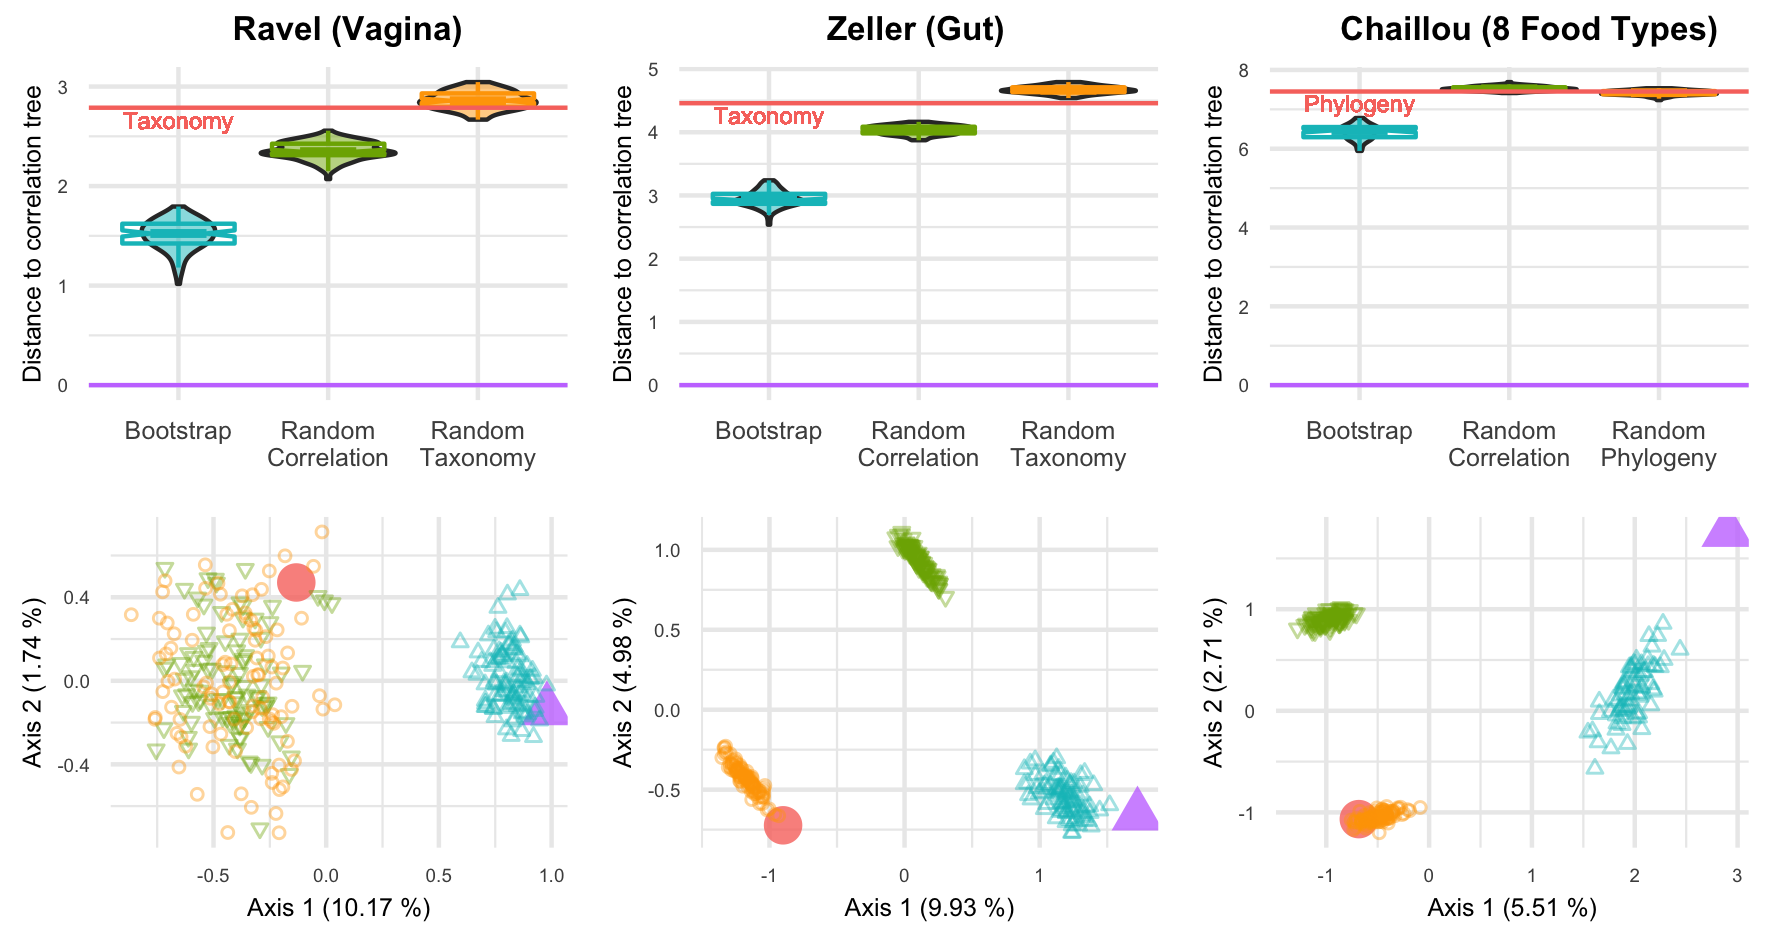
\includegraphics[width=0.9\linewidth]{img/foretbhv} 

}

\caption{Distances BHV au sein de la forêt d'arbres pour trois jeux de données.}\label{fig:foretbhv}
\end{figure}
Ces résultats doivent être mis en regard de ceux obtenus avec le jeu de données \emph{Chlamydiae} de Caporaso et al. (\protect\hyperlink{ref-caporaso2011global}{2011}), où la phylogénie se positionne au sein de la région de confiance de l'arbre des corrélations (figure \ref{fig:foretbhvbis}). Ce jeu de données se caractérise par sa faible taille : seulement \(26\) échantillons et beaucoup de taxons peu abondants ou peu prévalents, ce qui produit une région de confiance très large. De plus, il contient des échantillons provenant de \(8\) environnements très différents (océan, selles, sol\ldots), et ces niches écologiques se retrouvent à la fois dans la phylogénie (Philippot et al., \protect\hyperlink{ref-philippot2010ecological}{2010}) et dans l'arbre des corrélations.


\begin{figure}[t]

{\centering 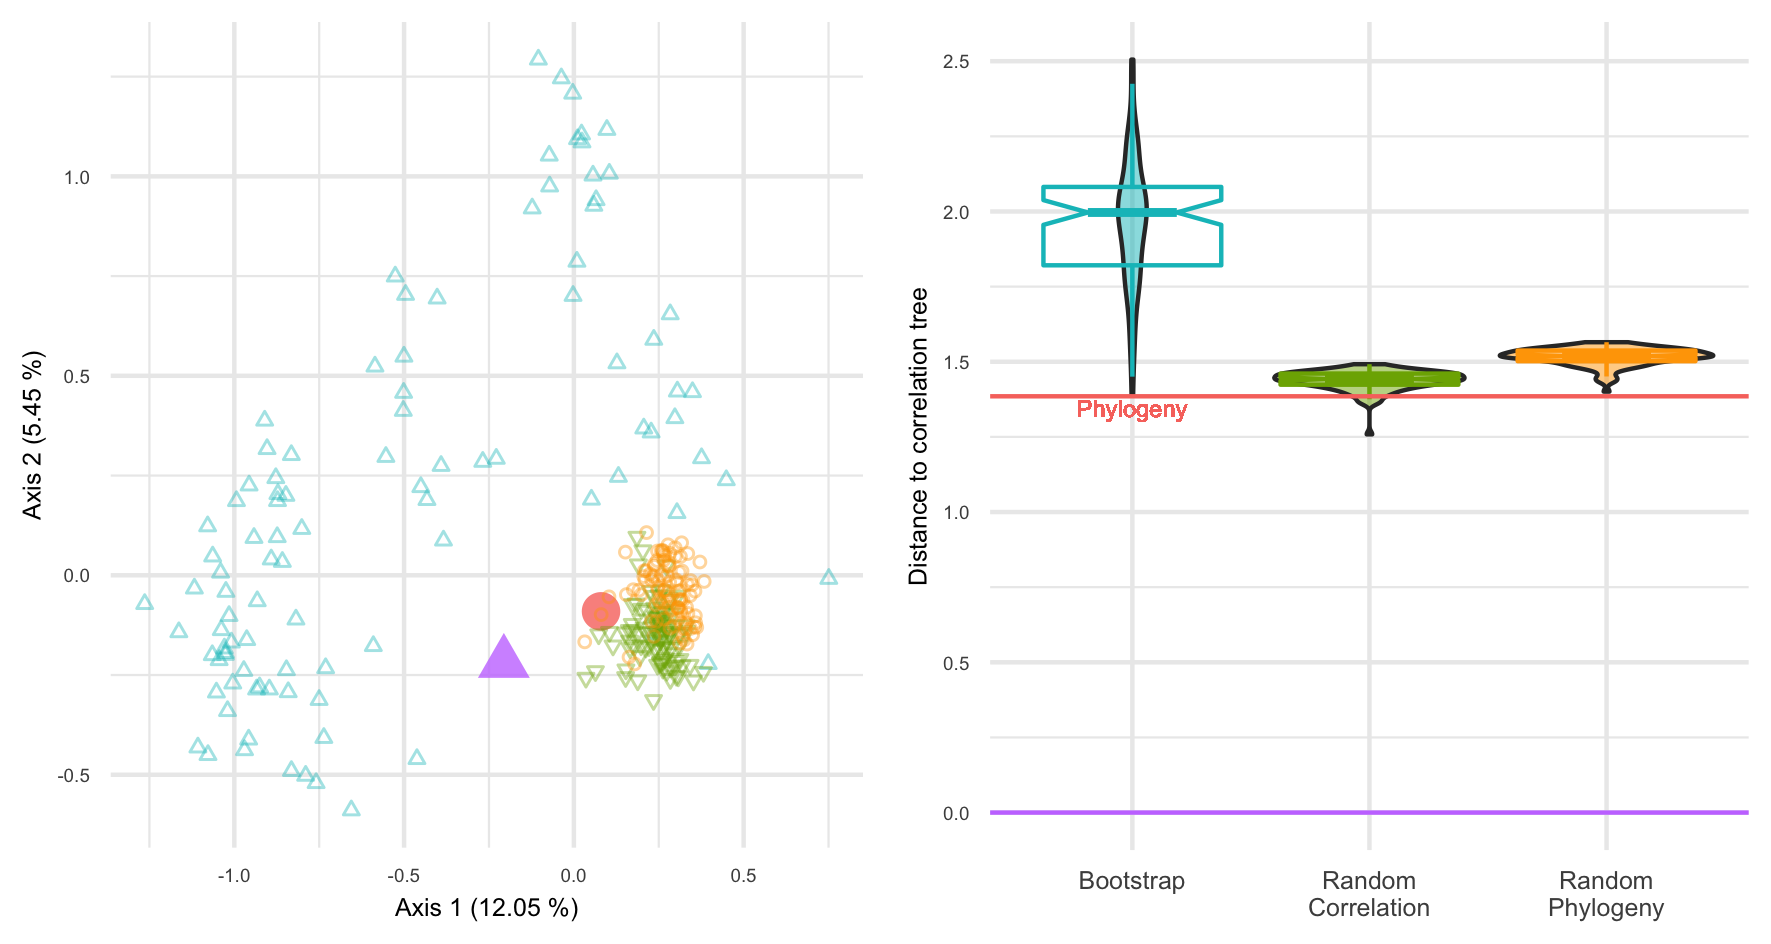
\includegraphics[width=0.9\linewidth]{img/foretbhv_ch} 

}

\caption{Distances BHV au sein de la forêt d'arbres pour le jeu de données Chlamydiae.}\label{fig:foretbhvbis}
\end{figure}
À l'aide de ces résultats, nous pouvons affirmer que l'arbre des corrélations ne capte pas le même signal que la taxonomie ou la phylogénie, en particulier lorsque l'on se concentre sur un seul biome. Les taxons avec un profil d'abondance similaire sont regroupés ensemble dans l'arbre des corrélations, par construction, mais pas dans la taxonomie ou la phylogénie, ce qui ne fait d'aucun de ces deux derniers arbres un bon candidat pour trouver des groupes de taxons différentiellement abondants.

Nous obtenons les mêmes conclusions en utilisant la distance RF, comme le montre la figure \ref{fig:foretrf}.


\begin{figure}

{\centering 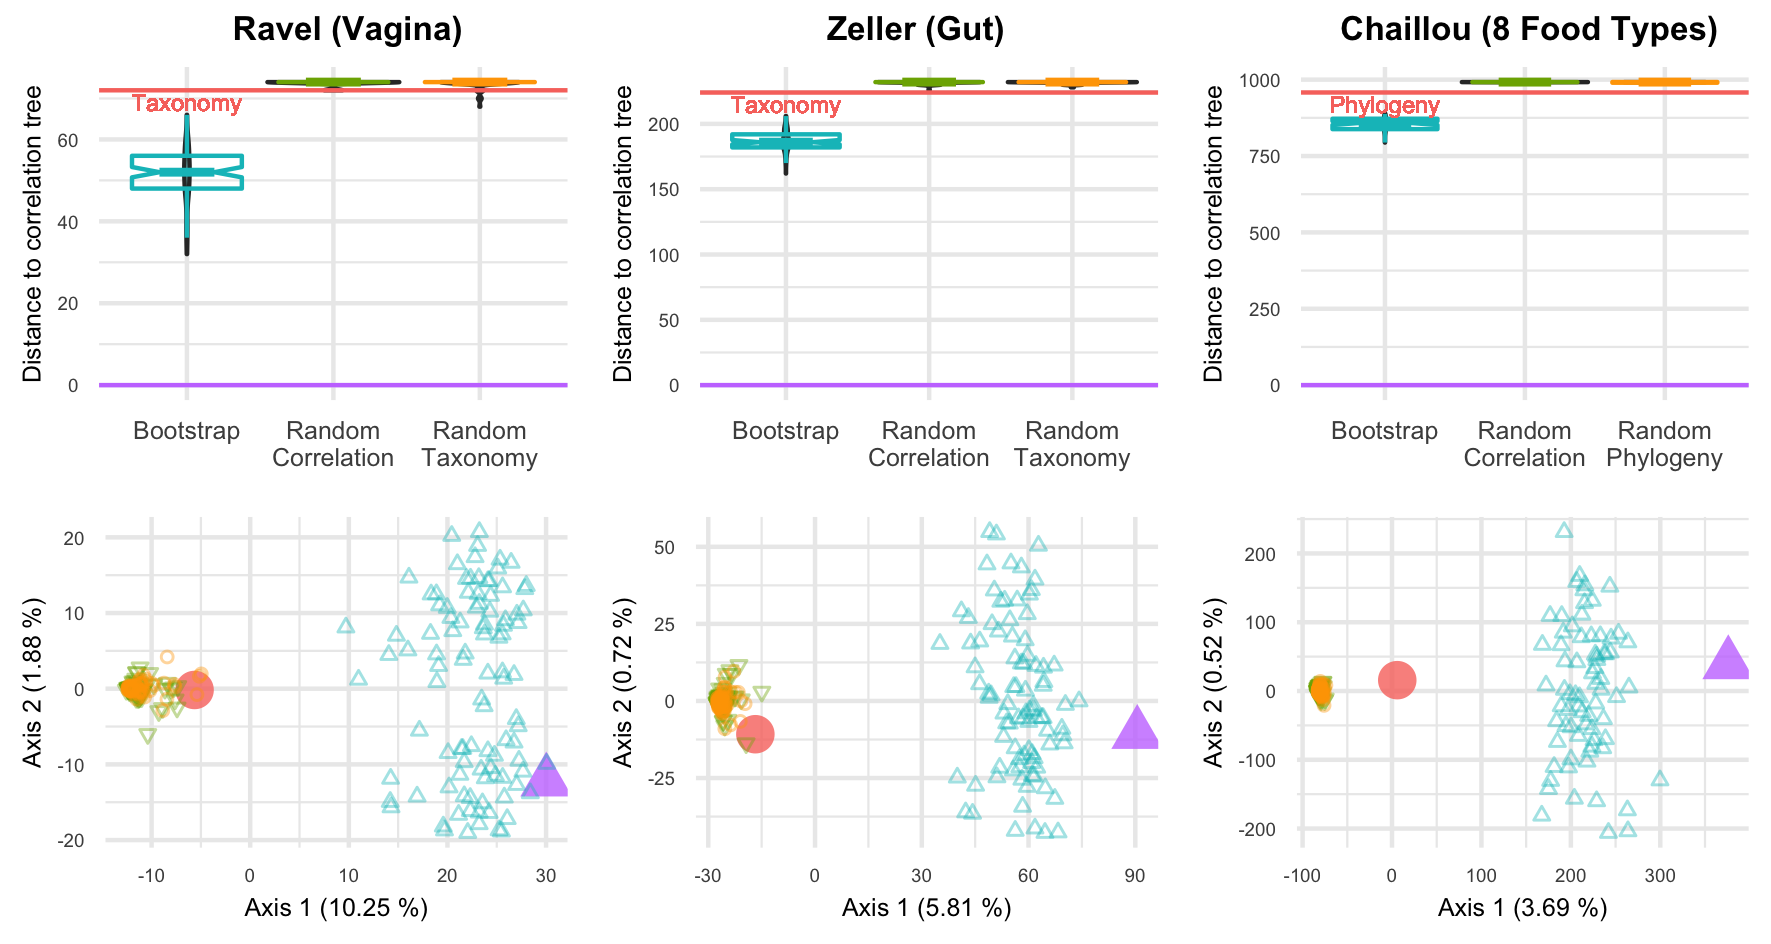
\includegraphics[width=0.9\linewidth]{img/foretrf} 

}

\caption{Distances RF au sein de la forêt d'arbres pour trois jeux de données.}\label{fig:foretrf}
\end{figure}
\hypertarget{checktreefdr}{%
\subsection{Choix de l'arbre et lissage de z-score}\label{checktreefdr}}

L'arbre des corrélations étant différent de l'arbre taxonomique, nous avons regardé l'impact du choix de l'arbre sur la procédure \emph{TreeFDR} (Xiao et al., \protect\hyperlink{ref-xiao2017false}{2017}), à la fois sur des données simulées et sur un jeu de données réel.

Afin de simuler un jeu de données métagénomique, nous avons d'abord appris du jeu de données de Wu et al. (\protect\hyperlink{ref-wu2011linking}{2011}) les paramètres d'une loi Dirichlet-multinomiale \(\mathcal{D}(\gamma)\). Nous créons ensuite un jeu de données échantillon par échantillon comme suit : (i) la profondeur de séquençage \(N_i\) est tirée selon une loi binomiale négative de moyenne \(10000\) et de dispersion \(25\), (ii) le vecteur de proportion \(\alpha_i\) est tirée dans une distribution de Dirichlet de paramètre \(\gamma\) puis (iii) les comptages de l'échantillon \(i\) sont tirés dans une loi multinomiale de paramètre \(N_i\) et \(\alpha_i\).

Une fois le jeu de données simulées obtenu, il reste à créer des taxons différentiellement abondants. La procédure est illustrée dans la figure \ref{fig:abdiff}. Tout d'abord, les échantillons sont aléatoirement assignés à un groupe \(A\) ou \(B\) (quadrant B). Ensuite, les taxons différentiellement abondants sont sélectionnés uniformément dans l'arbre (quadrant C). Enfin, l'abondance de ces taxons au sein du groupe \(B\) est multipliée par un \emph{fold-change} (quadrant D).


\begin{figure}[!t]

{\centering 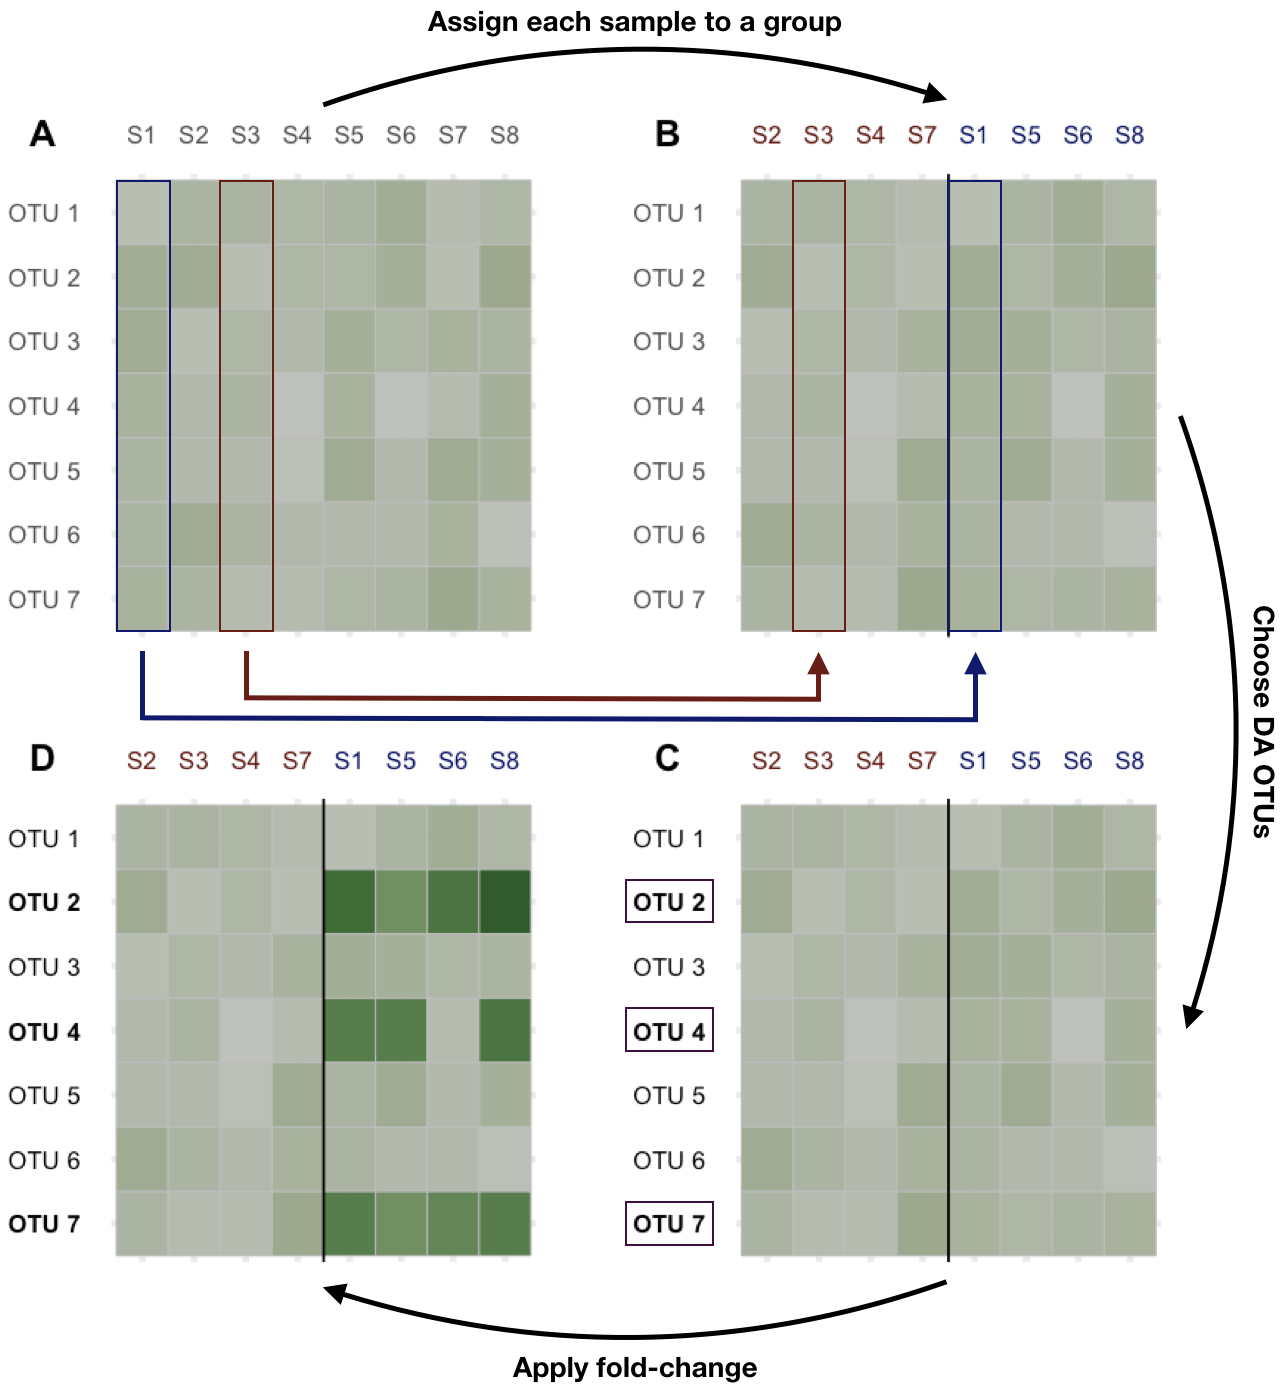
\includegraphics[width=0.9\linewidth]{img/abdiff} 

}

\caption{Création de taxons différentiellement abondants au sein d'un jeu de données.}\label{fig:abdiff}
\end{figure}
On qualifiera ce schéma de simulation de \emph{paramétrique}.

Il est également possible d'utiliser directement les comptages d'un jeu de données réel homogène, comme celui des individus sains de Brito et al. (\protect\hyperlink{ref-brito2016mobile}{2016}) --au lieu d'en simuler suivant une Dirichlet-multinomiale-- puis d'appliquer la procédure de la figure \ref{fig:abdiff} pour générer de l'abondance différentielle. On parlera alors d'un schéma \emph{non-paramétrique} --par opposition à la simulation paramétrique, précédemment décrite.

Nous avons généré des jeux de données d'abondance différentielle puis évalué la performance des corrections Benjamin-Hochberg et de \emph{TreeFDR} avec l'arbre des corrélations, la taxonomie, un arbre des corrélations aléatoire et une taxonomie aléatoire.

Regardons dans un premier temps les simulations non paramétriques (issues d'un jeu de données réelles). Tout d'abord, notons que la procédure échoue dans \(4~\%\) des simulations pour l'ensemble des arbres, et jusqu'à \(8~\%\) quand on se limite à l'arbre des corrélations. Notons ensuite que les hyperparamètres \(k\) et \(\rho\) qui contrôlent le niveau de lissage des \(z\)-scores sont assez éloignés de \(1\) (très bas pour \(k\), très haut pour \(\rho\)), ce qui réduit considérablement l'impact du lissage. Les distributions de la figure \ref{fig:smoothing} montrent que dans plus de la moitié des simulations, le lissage déplace le \(z\)-score de moins de \(10^{-2}\). Dans le cas où l'arbre utilisé est celui des corrélations, un déplacement des \(z\)-scores d'amplitude supérieure à \(10^{-2}\) ne se produit que dans \(5~\%\) des simulations.


\begin{figure}

{\centering 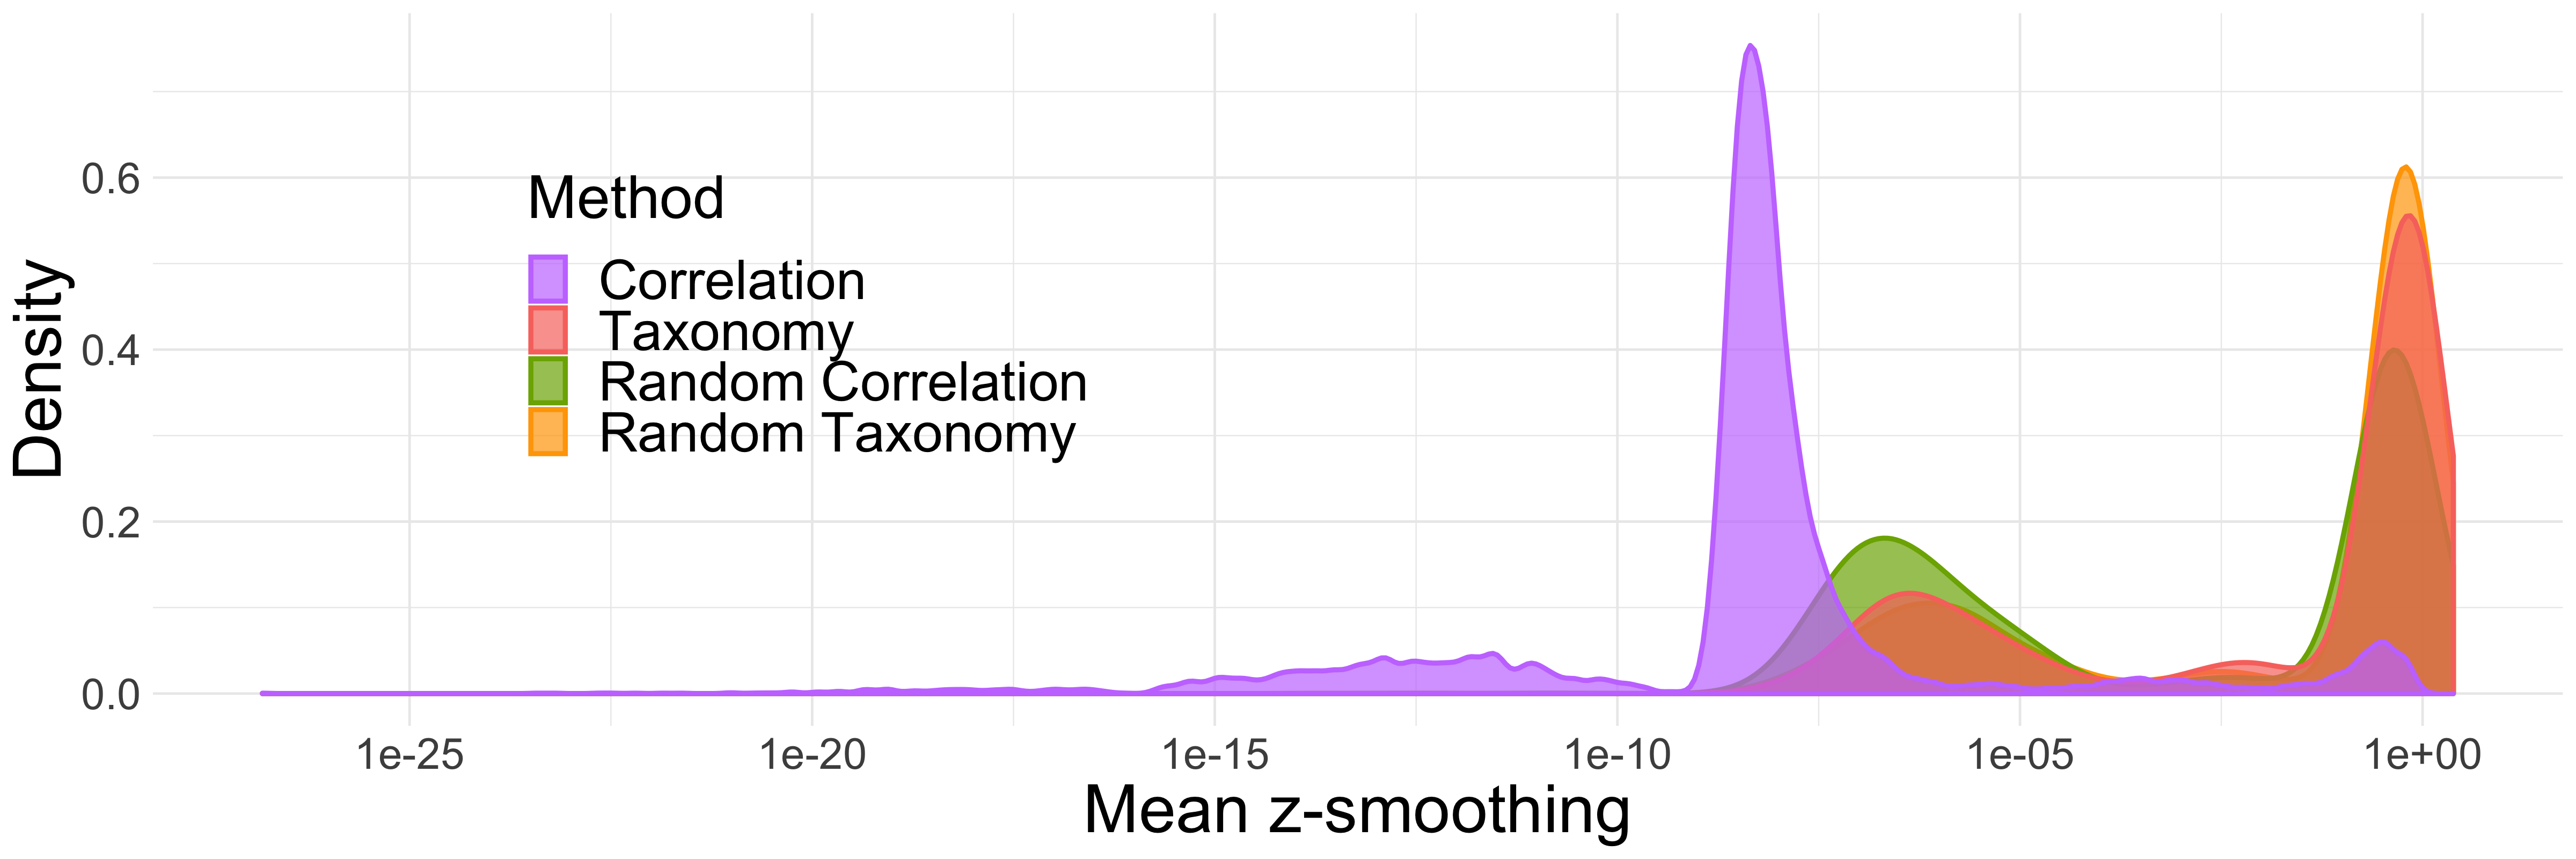
\includegraphics[width=0.9\linewidth]{img/smoothing} 

}

\caption{Distribution des moyennes des valeurs absolues des différences entres les \(z\)-scores avant et après lissage, pour les simulations non paramétriques.}\label{fig:smoothing}
\end{figure}
Au niveau du contrôle du FDR, seul BH contrôle systématiquement le taux de faux positifs en deçà de \(5~\%\) (figure \ref{fig:tprfdrcornp} bas). Les procédures hiérarchiques peuvent dépasser ce seuil, allant jusqu'à \(7~\%\) lorsque la proportion réelle d'espèces différentiellement abondantes est faible (\(\leq 10~\%\)). Enfin, BH est la méthode qui a le plus important TPR, quelque soit le \emph{fold-change} ou la proportion d'hypothèses nulles (figure \ref{fig:tprfdrcornp} haut). Devant ces résultats, nous pouvons affirmer que l'utilisation d'un arbre dans la procédure de lissage de \emph{TreeFDR}, même adapté aux données d'abondances comme l'arbre des corrélations, ne permet pas d'avoir des procédures plus puissantes que BH.


\begin{figure}[!t]

{\centering 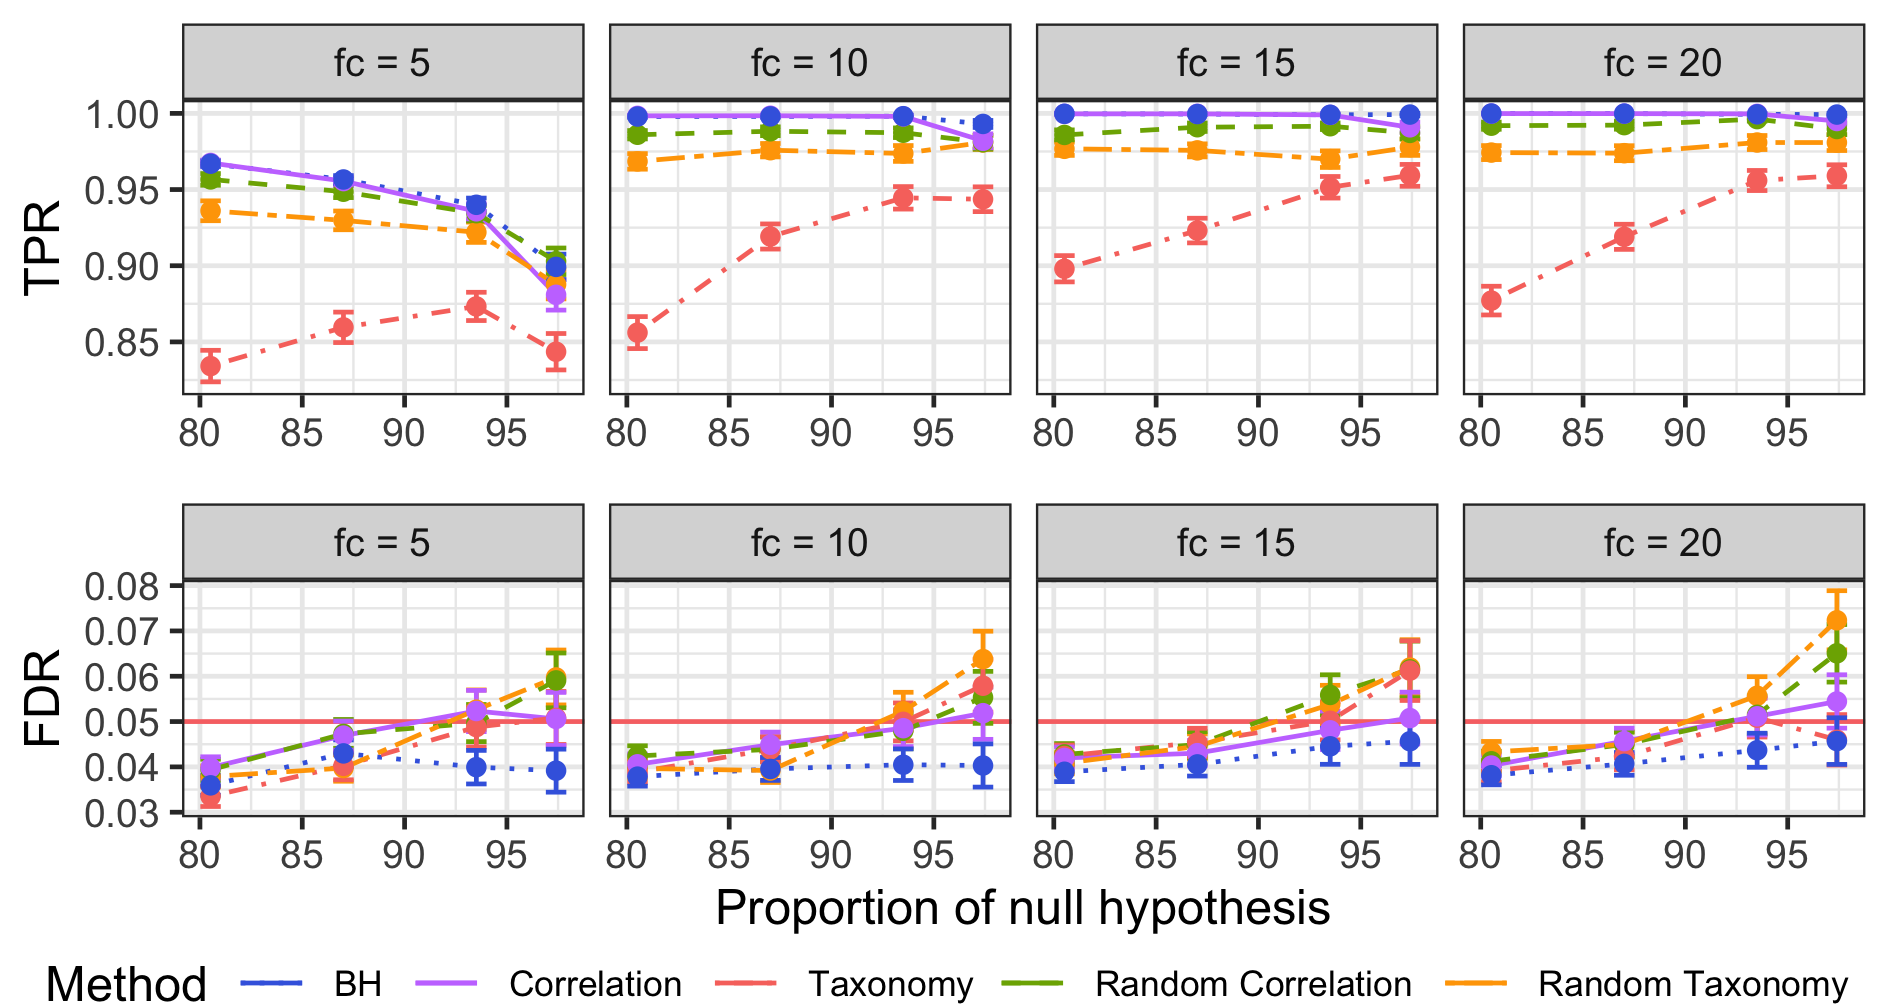
\includegraphics[width=0.9\linewidth]{img/tprfdr_cor_np} 

}

\caption{Moyennes et écart-types de la moyenne des TPR et FDR pour les simulations non paramétriques avec différents \emph{fold-changes} et proportions d'hypothèses nulles.}\label{fig:tprfdrcornp}
\end{figure}
Les simulations paramétriques donnent des résultats semblables aux simulations non-paramétriques, comme le montre la figure \ref{fig:tprfdrcorp}. On note cependant un effondrement du TPR avec ce schéma de simulation.


\begin{figure}[!t]

{\centering 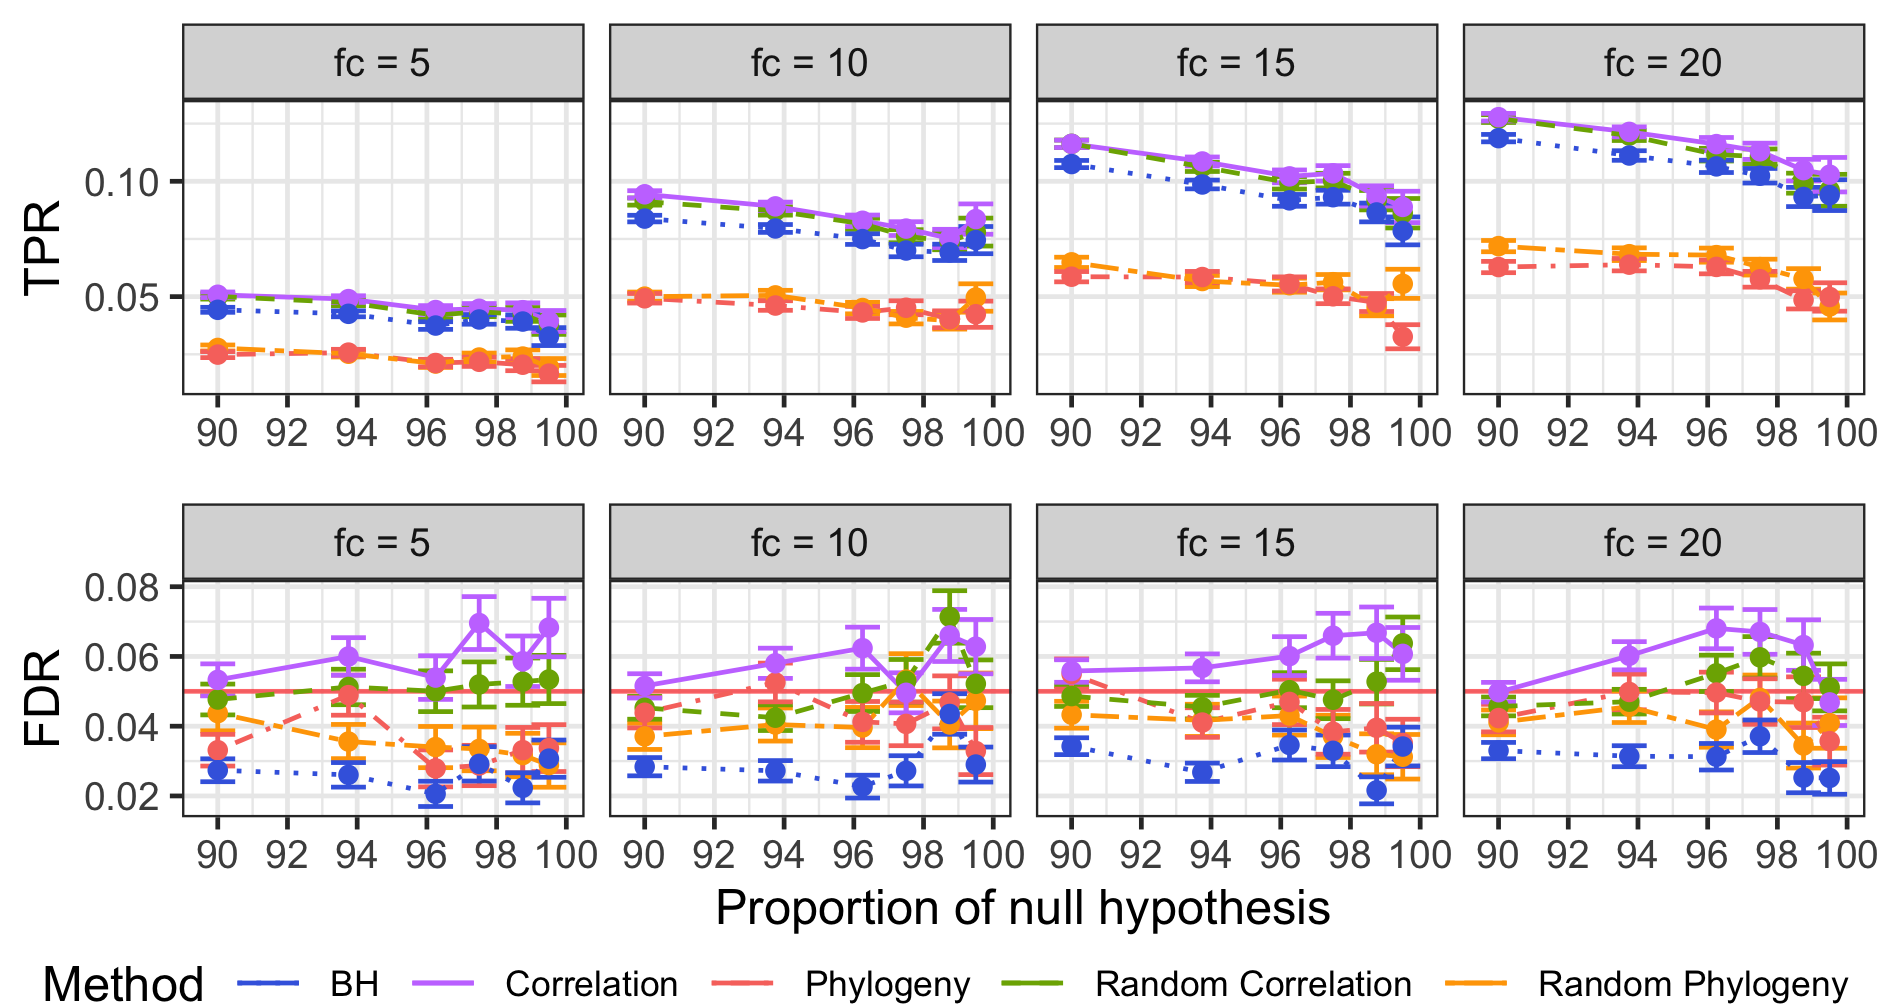
\includegraphics[width=0.9\linewidth]{img/tprfdr_cor_p} 

}

\caption{Moyennes et écart-types de la moyenne des TPR et FDR pour les simulations paramétriques avec différents \emph{fold-changes} et proportions d'hypothèses nulles.}\label{fig:tprfdrcorp}
\end{figure}
Nous avons également testé l'influence de l'arbre sur la procédure de lissage avec le jeu de données de Zeller et al. (\protect\hyperlink{ref-zeller2014potential}{2014}). Celui-ci a été analysé à deux niveaux de granularité différents : genre et MSP. La figure montre le nombre de genres (à gauche) ou de MSPs (à droite) détectés pour différents seuils jusqu'à \(\alpha = 0.15\).


\begin{figure}[!b]

{\centering 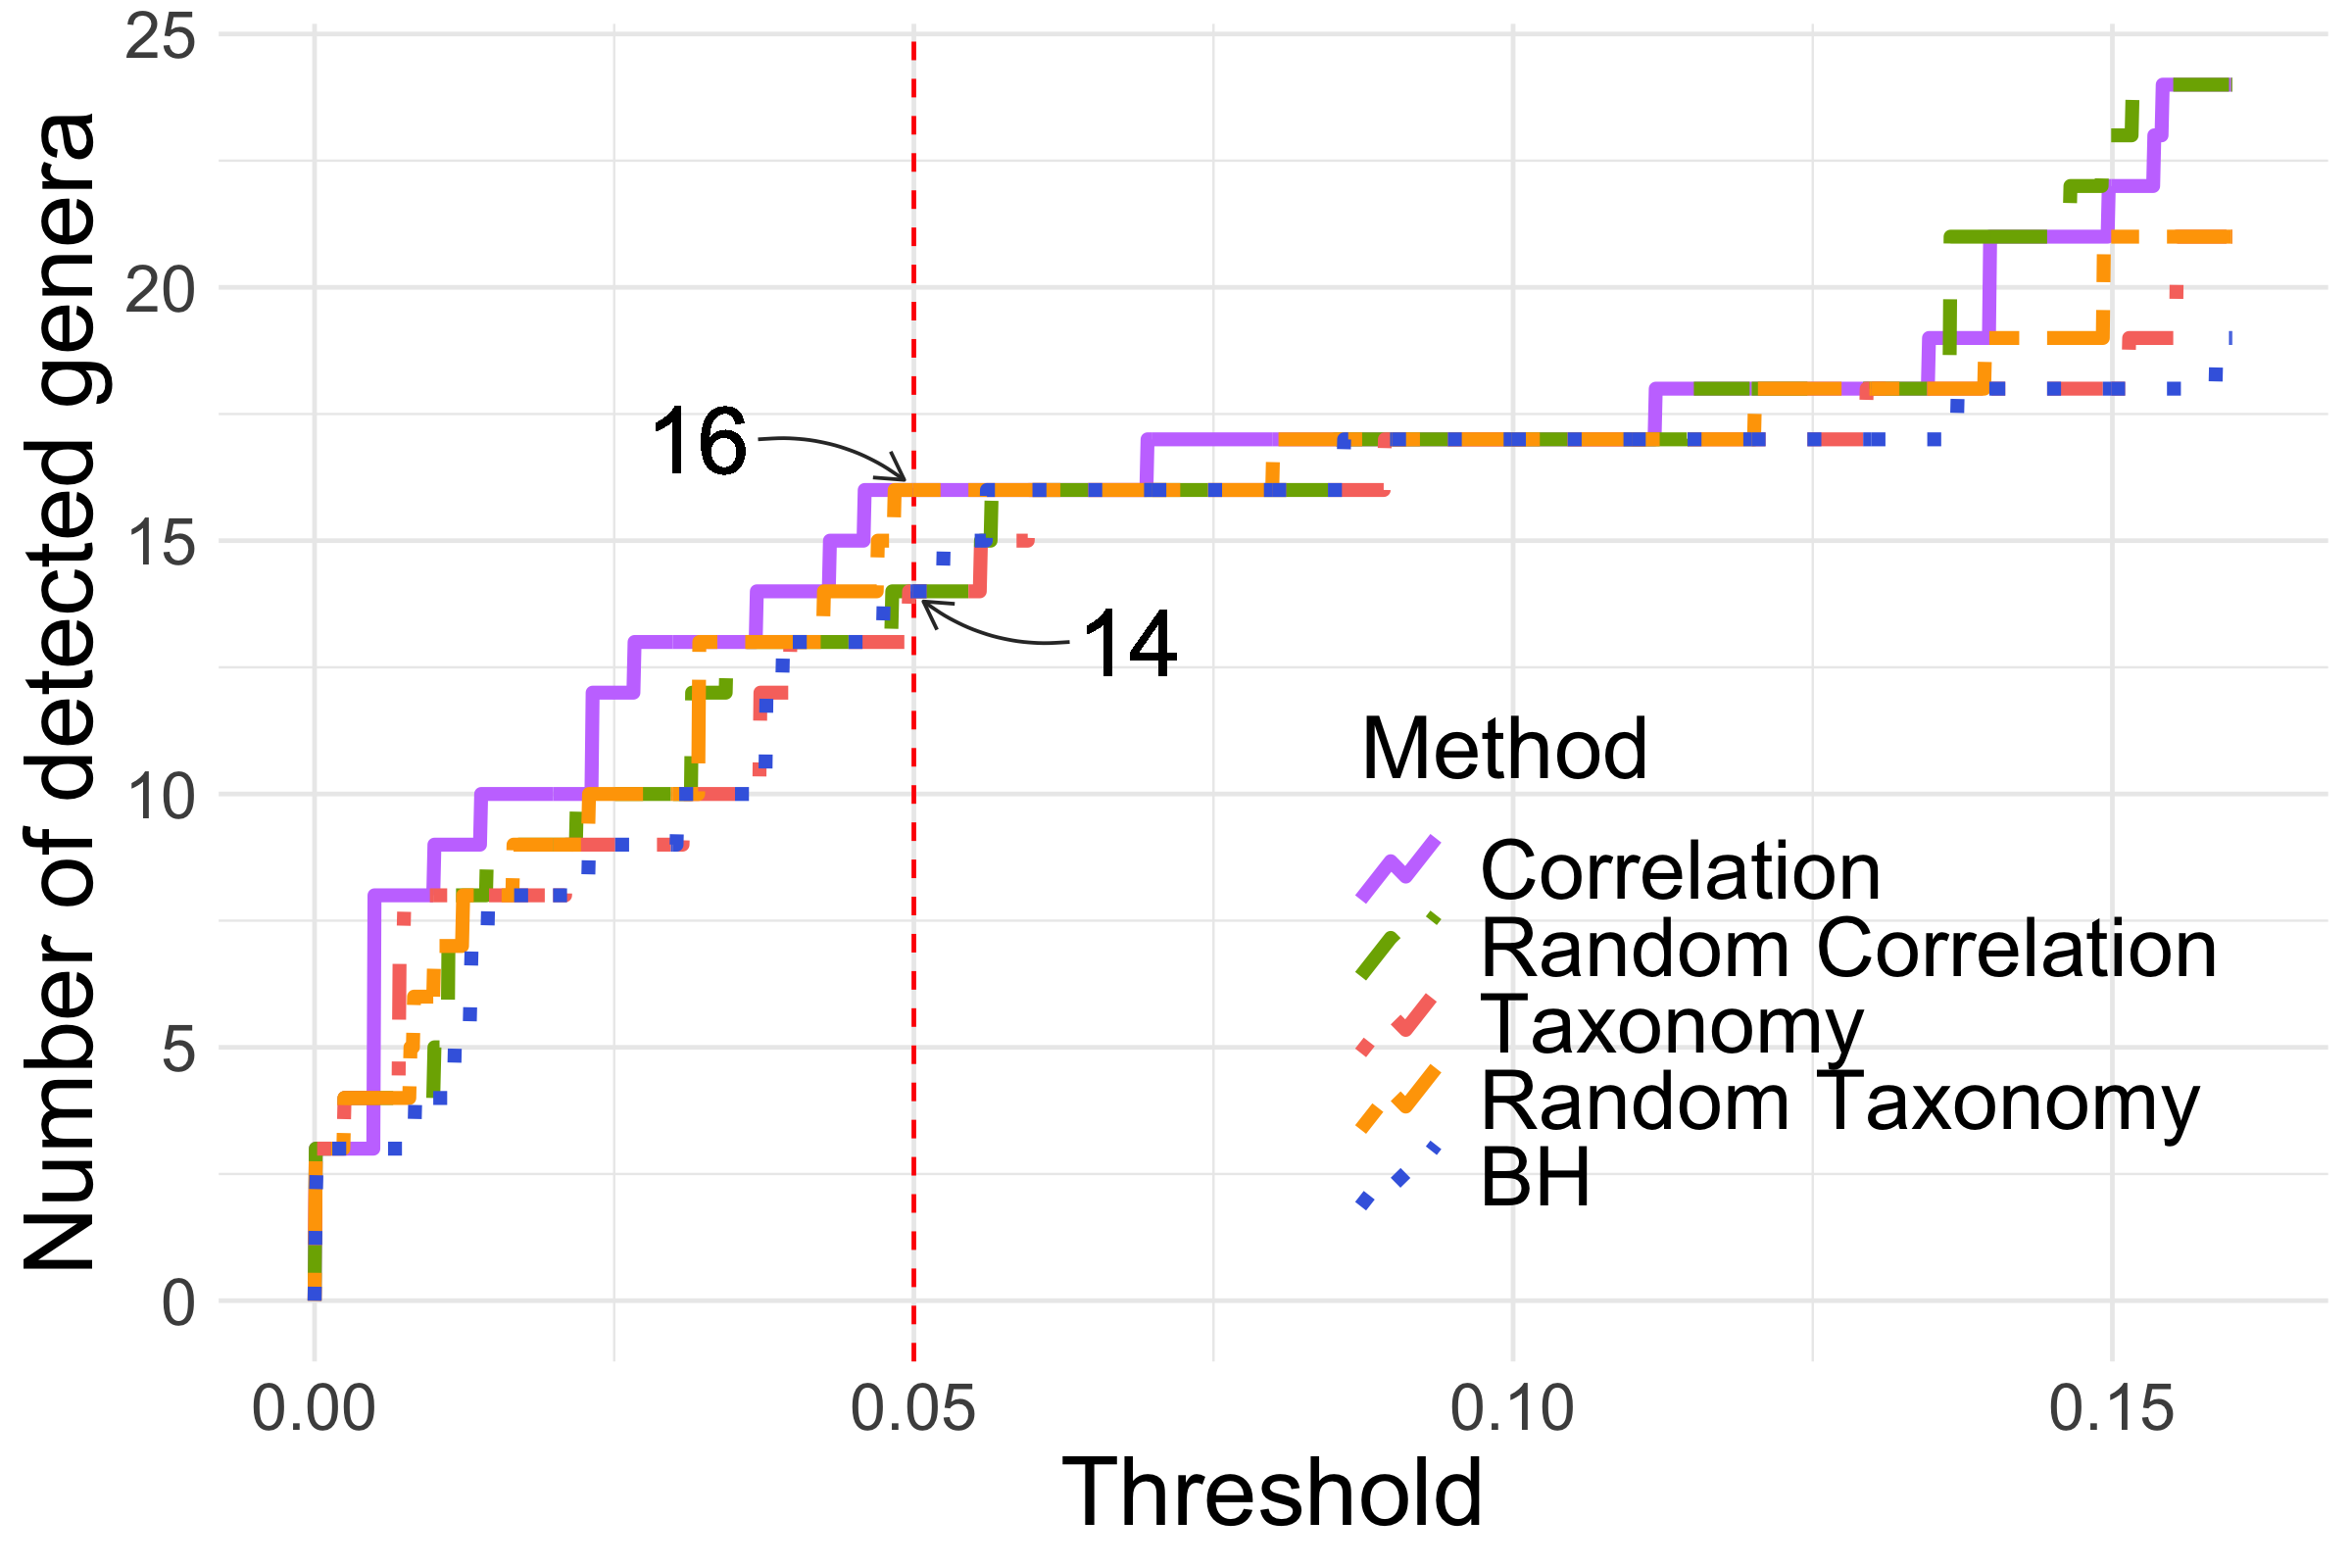
\includegraphics[width=0.4\linewidth]{img/zeller_detect_genus} 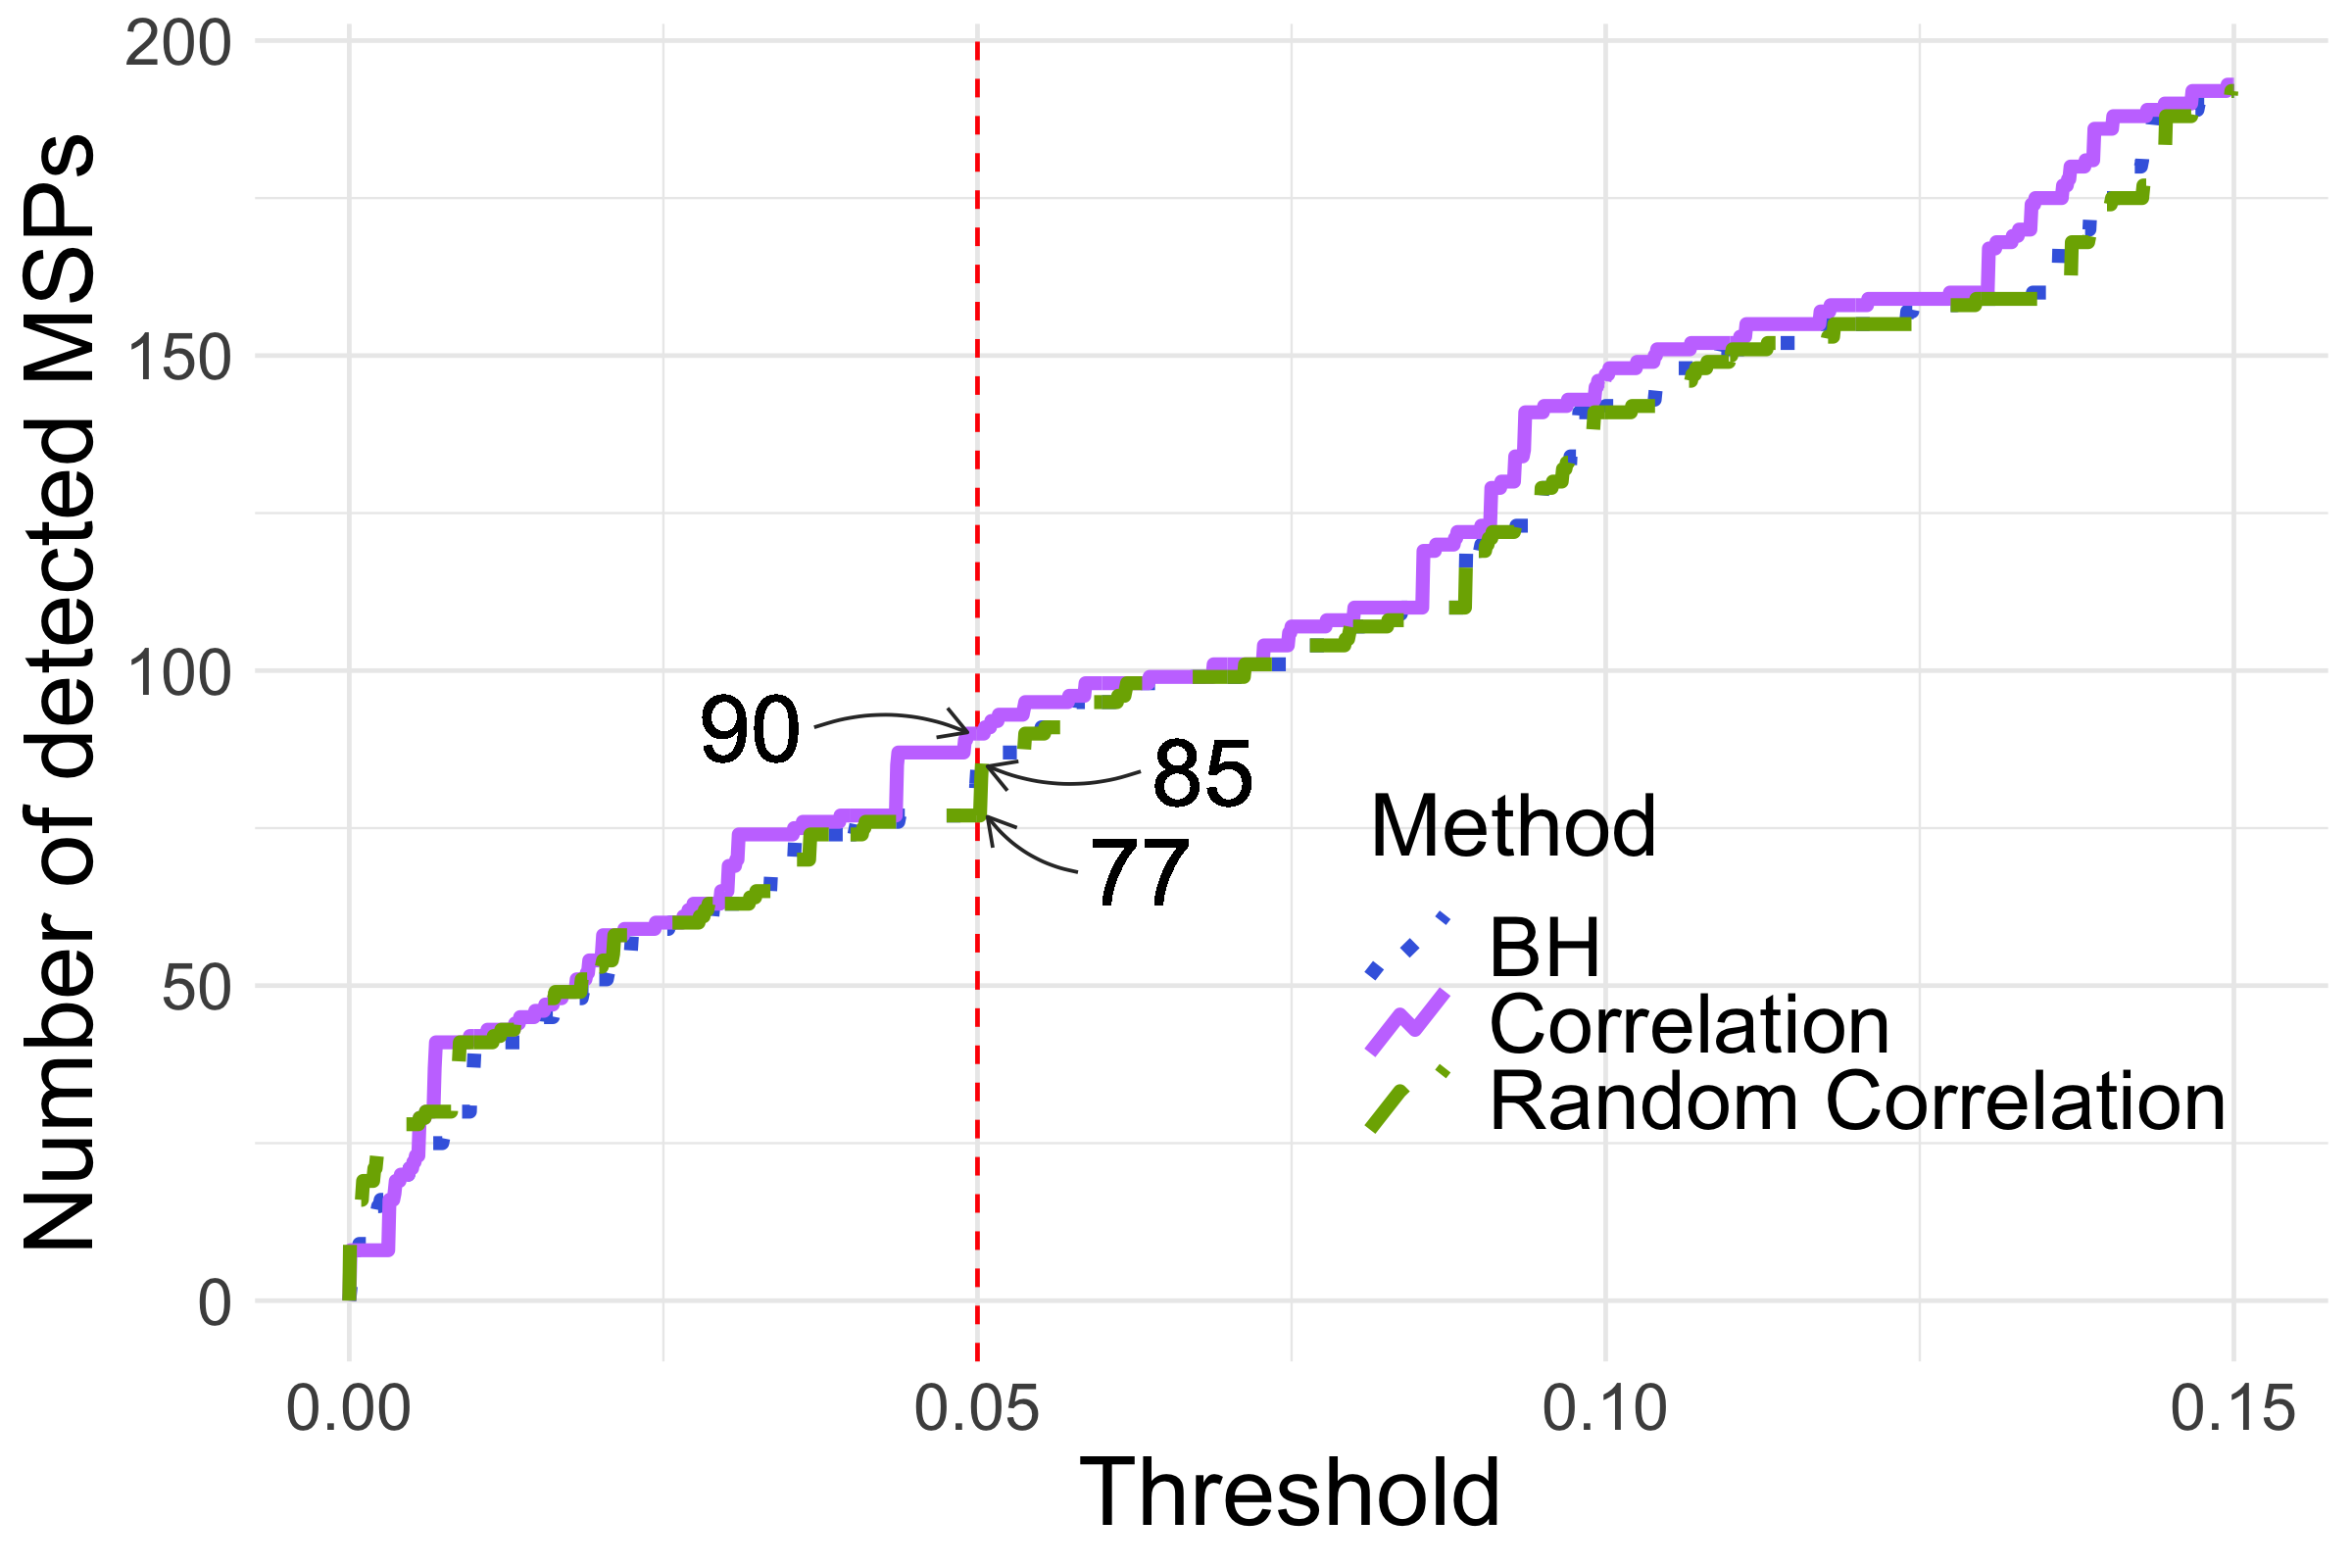
\includegraphics[width=0.4\linewidth]{img/zeller_detect_msp} 

}

\caption{Moyennes et écart-types de la moyenne des TPR et FDR pour les simulations non paramétriques avec différents \emph{fold-changes} et proportions d'hypothèses nulles.}\label{fig:zellerdetected}
\end{figure}
Dans les deux cas, l'arbre des corrélations détecte pour la majorité des seuils plus de taxons que BH mais la différence est très faible, y compris en comparaison avec les arbres aléatoires. Si l'on regarde au niveau des MSPs à \(\alpha = 0.05\), l'arbre des corrélations permet de détecter 5 taxons de plus que la procédure BH classique. Ces taxons ne sont cependant pas regroupés dans des clades différentiellement abondants. Il semblerait alors que cela soit plutôt la correction de permutation post-lissage, qui a pour objectif de contrôler le \emph{FDR discret}, plutôt que le lissage lui-même qui produise cet effet. Le FDR discret prend en compte des distributions non continues des \(p\)-valeurs sous l'hypothèse nulle et est adapté aux données de comptage. Cette méthode de correction a été déclarée plus performante pour détecter des taxons différentiellement abondants que la procédure BH classique (Jiang et al., \protect\hyperlink{ref-jiang2017discrete}{2017}).

\hypertarget{choix-de-larbre-et-fdr-hiuxe9rarchique}{%
\subsection{Choix de l'arbre et FDR hiérarchique}\label{choix-de-larbre-et-fdr-hiuxe9rarchique}}

Le fait que le FDR hiérarchique ne permette pas de spécifier \emph{a priori} un niveau de FDR cible mais uniquement de le calculer \emph{a posteriori} pour une liste d'espèces différentiellement abondantes le rend inadapté à des simulations comme celles de la section \ref{checktreefdr}. C'est pourquoi nous ne regarderons l'impact du choix de l'arbre sur cette procédure qu'au travers de jeux de données réelles.

Nous avons d'abord réanalysé le jeu de données Chlamydiae (Sankaran \& Holmes, \protect\hyperlink{ref-sankaran2014structssi}{2014}), comme dans l'article original, en utilisant un seuil pour la correction au niveau des familles \(\alpha = 0.1\). Avec la phylogénie, \(8\) OTUs ont été détectés comme différentiellement abondantes et la procédure garantit un FDR \emph{a posteriori} de \(\alpha'=0.32\). Si l'on utilise l'arbre des corrélations à la place, on trouve \(3\) OTUs supplémentaires pour un FDR \emph{a posteriori} comparable de \(\alpha'=0.324\). Les boîtes à moustaches des abondances de ces OTUs (figure \ref{fig:chlamydiae} E, F) montrent qu'elles sont bien plus abondantes dans les échantillons de sol que dans les autres biomes, ce qui confirme leur statut d'OTU différentiellement abondante.

La figure \ref{fig:chlamydiae} résume cette analyse en indiquant quelles OTUs sont détectées avec l'une ou l'autre des méthodes et en précisant les évidences brutes (\(\mathfrak{e} = -\log\pv\)) correspondantes aux feuilles des arbres. Intéressons nous plus particulièrement à l'OTU \(547~579\) (marquée d'une étoile rouge) qui a été détectée par l'arbre des corrélations (figure \ref{fig:chlamydiae} D) mais pas par la phylogénie (figure \ref{fig:chlamydiae} A). Elle n'a pas été testée par la phylogénie car elle est entourée d'espèces non différentiellement abondantes qui masquent le signal (figure \ref{fig:chlamydiae} B). À l'inverse, dans l'arbre des corrélations (figure \ref{fig:chlamydiae} D), elle se situe dans un clade où toutes les OTUs sont différentiellement abondantes, ce qui permet à la procédure de rejeter tous les sous-arbres contenant \(547~579\) jusqu'à la feuille correspondant à \(547~579\), sans s'arrêter au niveau des branches internes.


\begin{figure}[!t]

{\centering 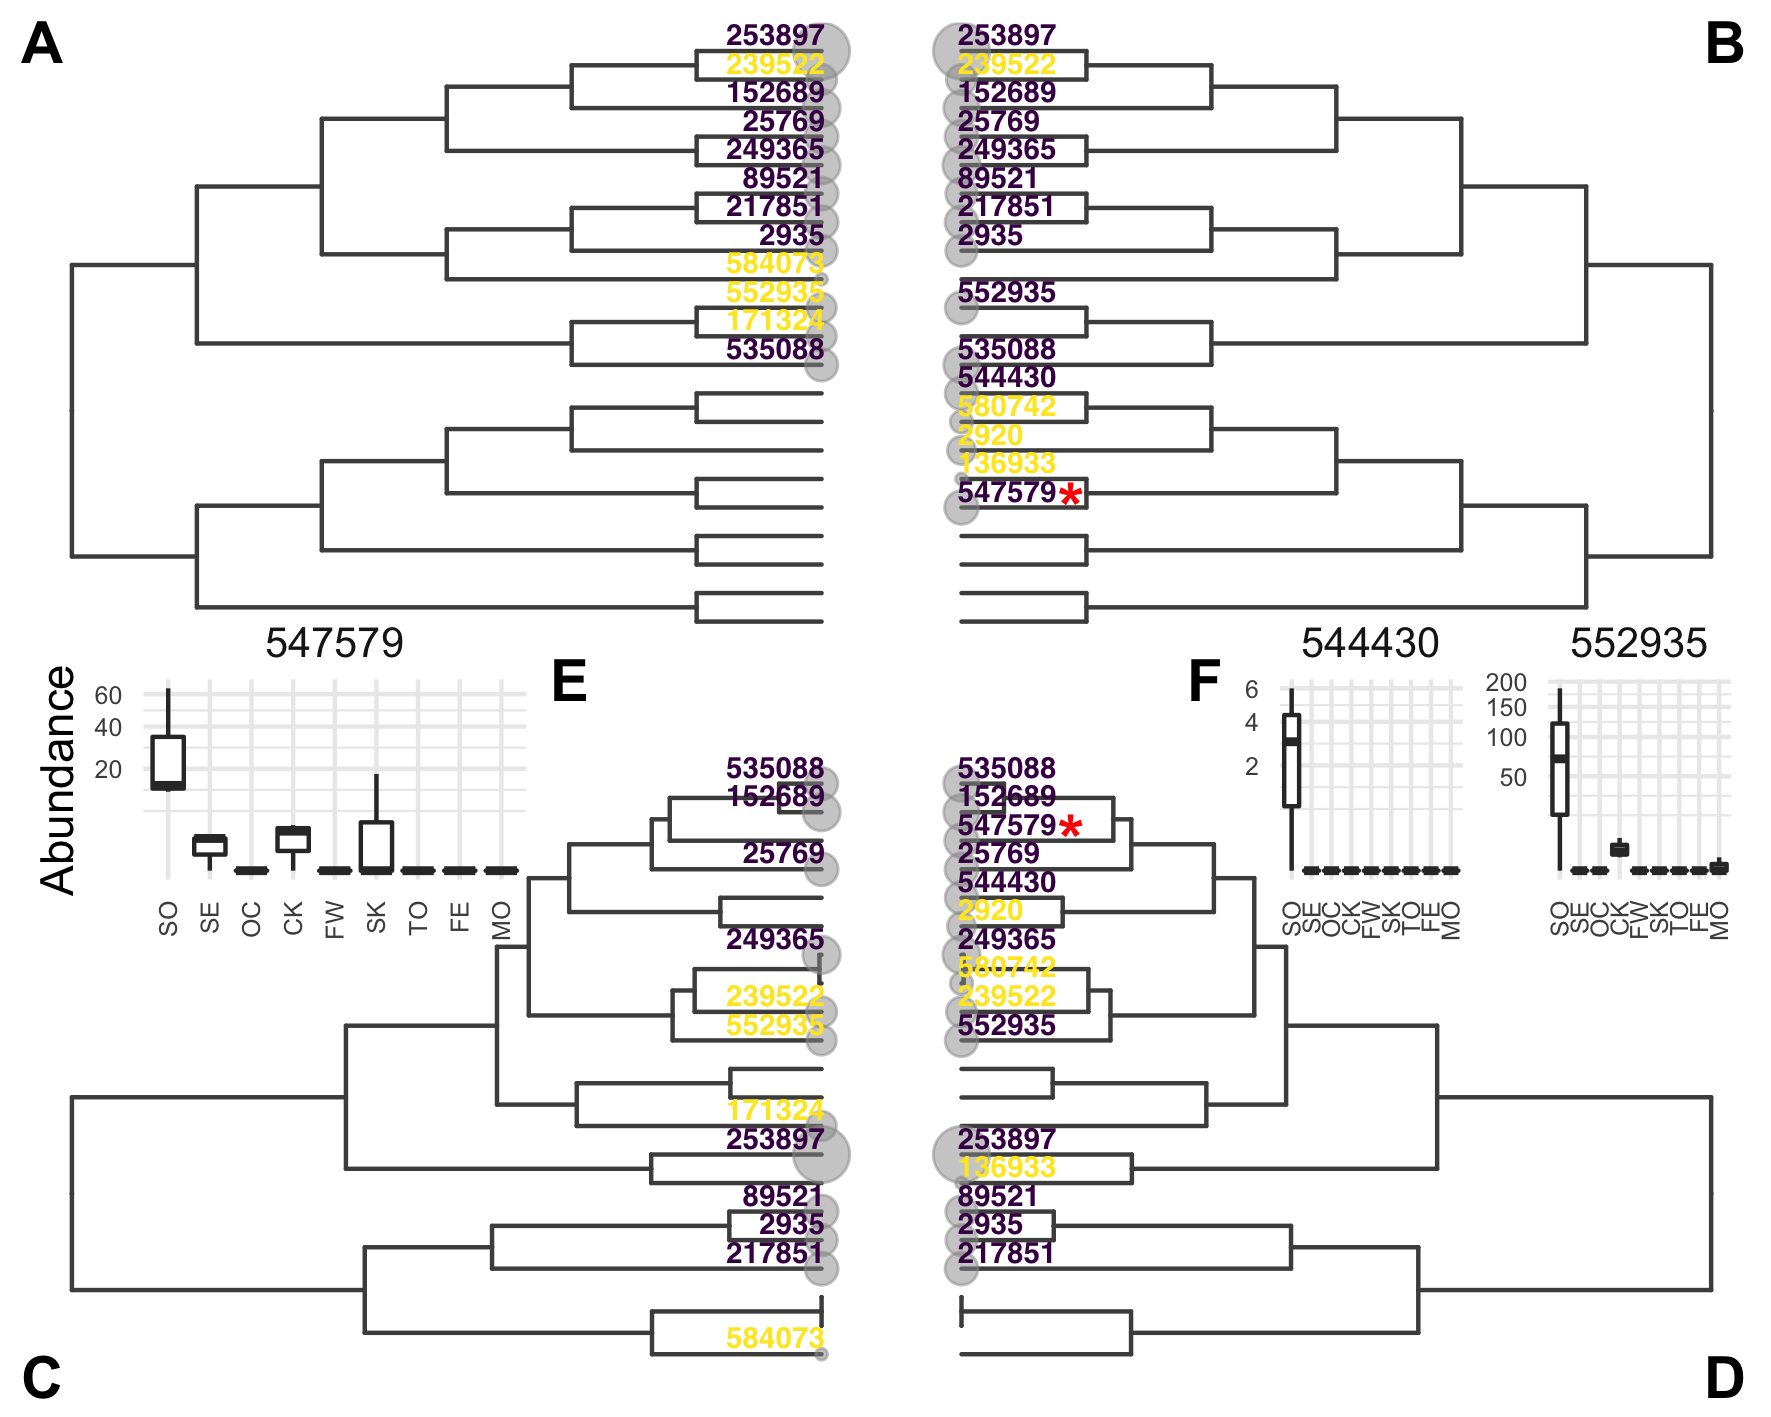
\includegraphics[width=0.9\linewidth]{img/chlamydiae} 

}

\caption{Les évidences brutes sont représentées aux feuilles de la phylogénie (A et C) ou de l'arbre des corrélations (B et D). Les OTUs considérées différentiellement abondantes pour la phylogénie (A et B) ou pour l'arbre des corrélations (C et D) sont en violet. Les OTUs testées mais non rejetées sont en jaune.}\label{fig:chlamydiae}
\end{figure}
On peut remarquer que le FDR \emph{a posteriori} est assez élevé, à \(0.324\). En effectuant une correction par BH à ce même niveau, on détecte \(15\) OTUs différentiellement abondantes, soit quatre de plus que la correction avec l'arbre des corrélations. Ceci peut s'expliquer par le fait que hFDR contrôle le FDR dans le pire des cas tandis que le FDR effectif pourrait être bien plus bas que cette borne pessimiste (Yekutieli, \protect\hyperlink{ref-yekutieli2008hierarchical}{2008}).

Avec cette approche descendante, l'arbre des corrélations est plus adapté que la phylogénie. En regroupant les espèces corrélées et donc potentiellement différentiellement abondantes au sein d'un même sous-arbre, il permet de concentrer les différents signaux dans une portion d'arbre et d'éviter qu'ils ne soient dilués dans tout l'arbre, comme c'est le cas avec la phylogénie.

Nous avons ensuite analysé le jeu de données Chaillou (Chaillou et al., \protect\hyperlink{ref-chaillou2015origin}{2015}) restreint aux \emph{Bacteroidetes}. L'utilisation d'un seuil \(\alpha=0.01\) au niveau des familles a conduit à un contrôle du FDR \emph{a posteriori} à \(\alpha'=0.04\) à la fois pour la phylogénie et l'arbre des corrélations. Le premier arbre a détecté \(28\) OTUs différentiellement abondantes contre \(34\) pour la phylogénie.

En observant l'abondance des \(22\) OTUs détectées simultanément par les deux procédures ou des \(18\) détectées par une seule des deux (figure \ref{fig:chailloubp}), on remarque que chacune d'entre elles (i) est absente ou en dessous du seuil de détection dans au moins un des aliments et (ii) a de fortes prévalences et abondances dans au moins un autre aliment. Ceci valide leur caractère différentiellement abondant et permet de les considérer comme des vrais positifs.


\begin{figure}

{\centering 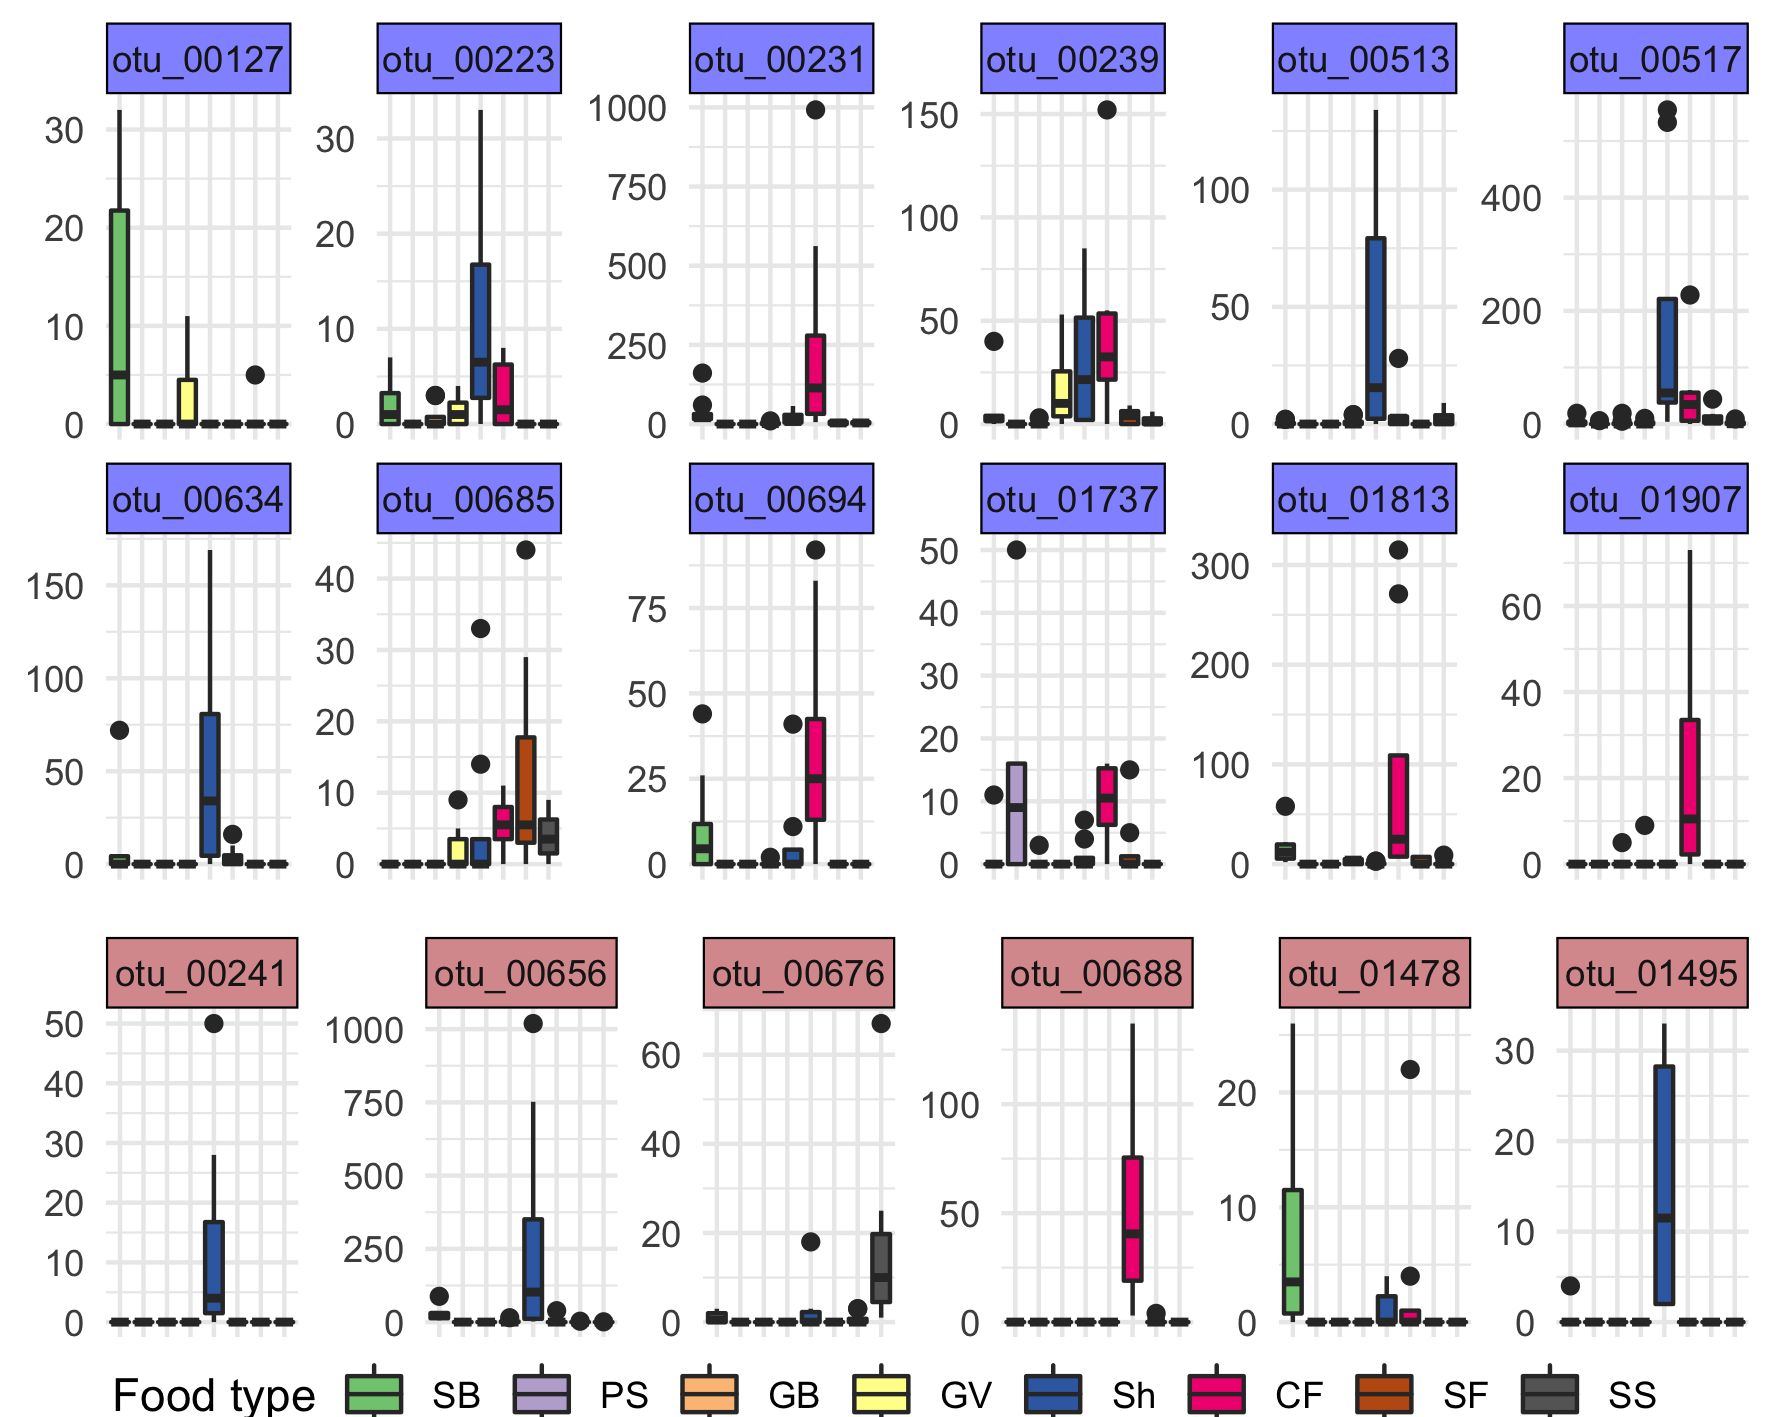
\includegraphics[width=0.9\linewidth]{img/chaillou_bp} 

}

\caption{Abondances des OTUs détectées uniquement par l'arbre des corrélations (en bleu) ou par la phylogénie (en rouge).}\label{fig:chailloubp}
\end{figure}
Si l'on regarde les OTUs détectées sur leurs arbres respectifs, comme représentées sur la figure \ref{fig:chailloutrees}, les OTUs détectées uniquement par l'arbre des corrélations sont éparpillées dans la phylogénie, de manière similaire à ce qu'on a pu observer pour le jeu de données Chlamydiae. À l'inverse, les OTUs différentiellement abondantes uniquement dans la phylogénie sont proches d'OTUs détectées pour l'arbre des corrélations mais ne sont pas détectées à cause de la faible puissance du test de Fisher, pratiqué par défaut dans \texttt{StructSSI} et peu adapté aux données métagénomiques.


\begin{figure}

{\centering 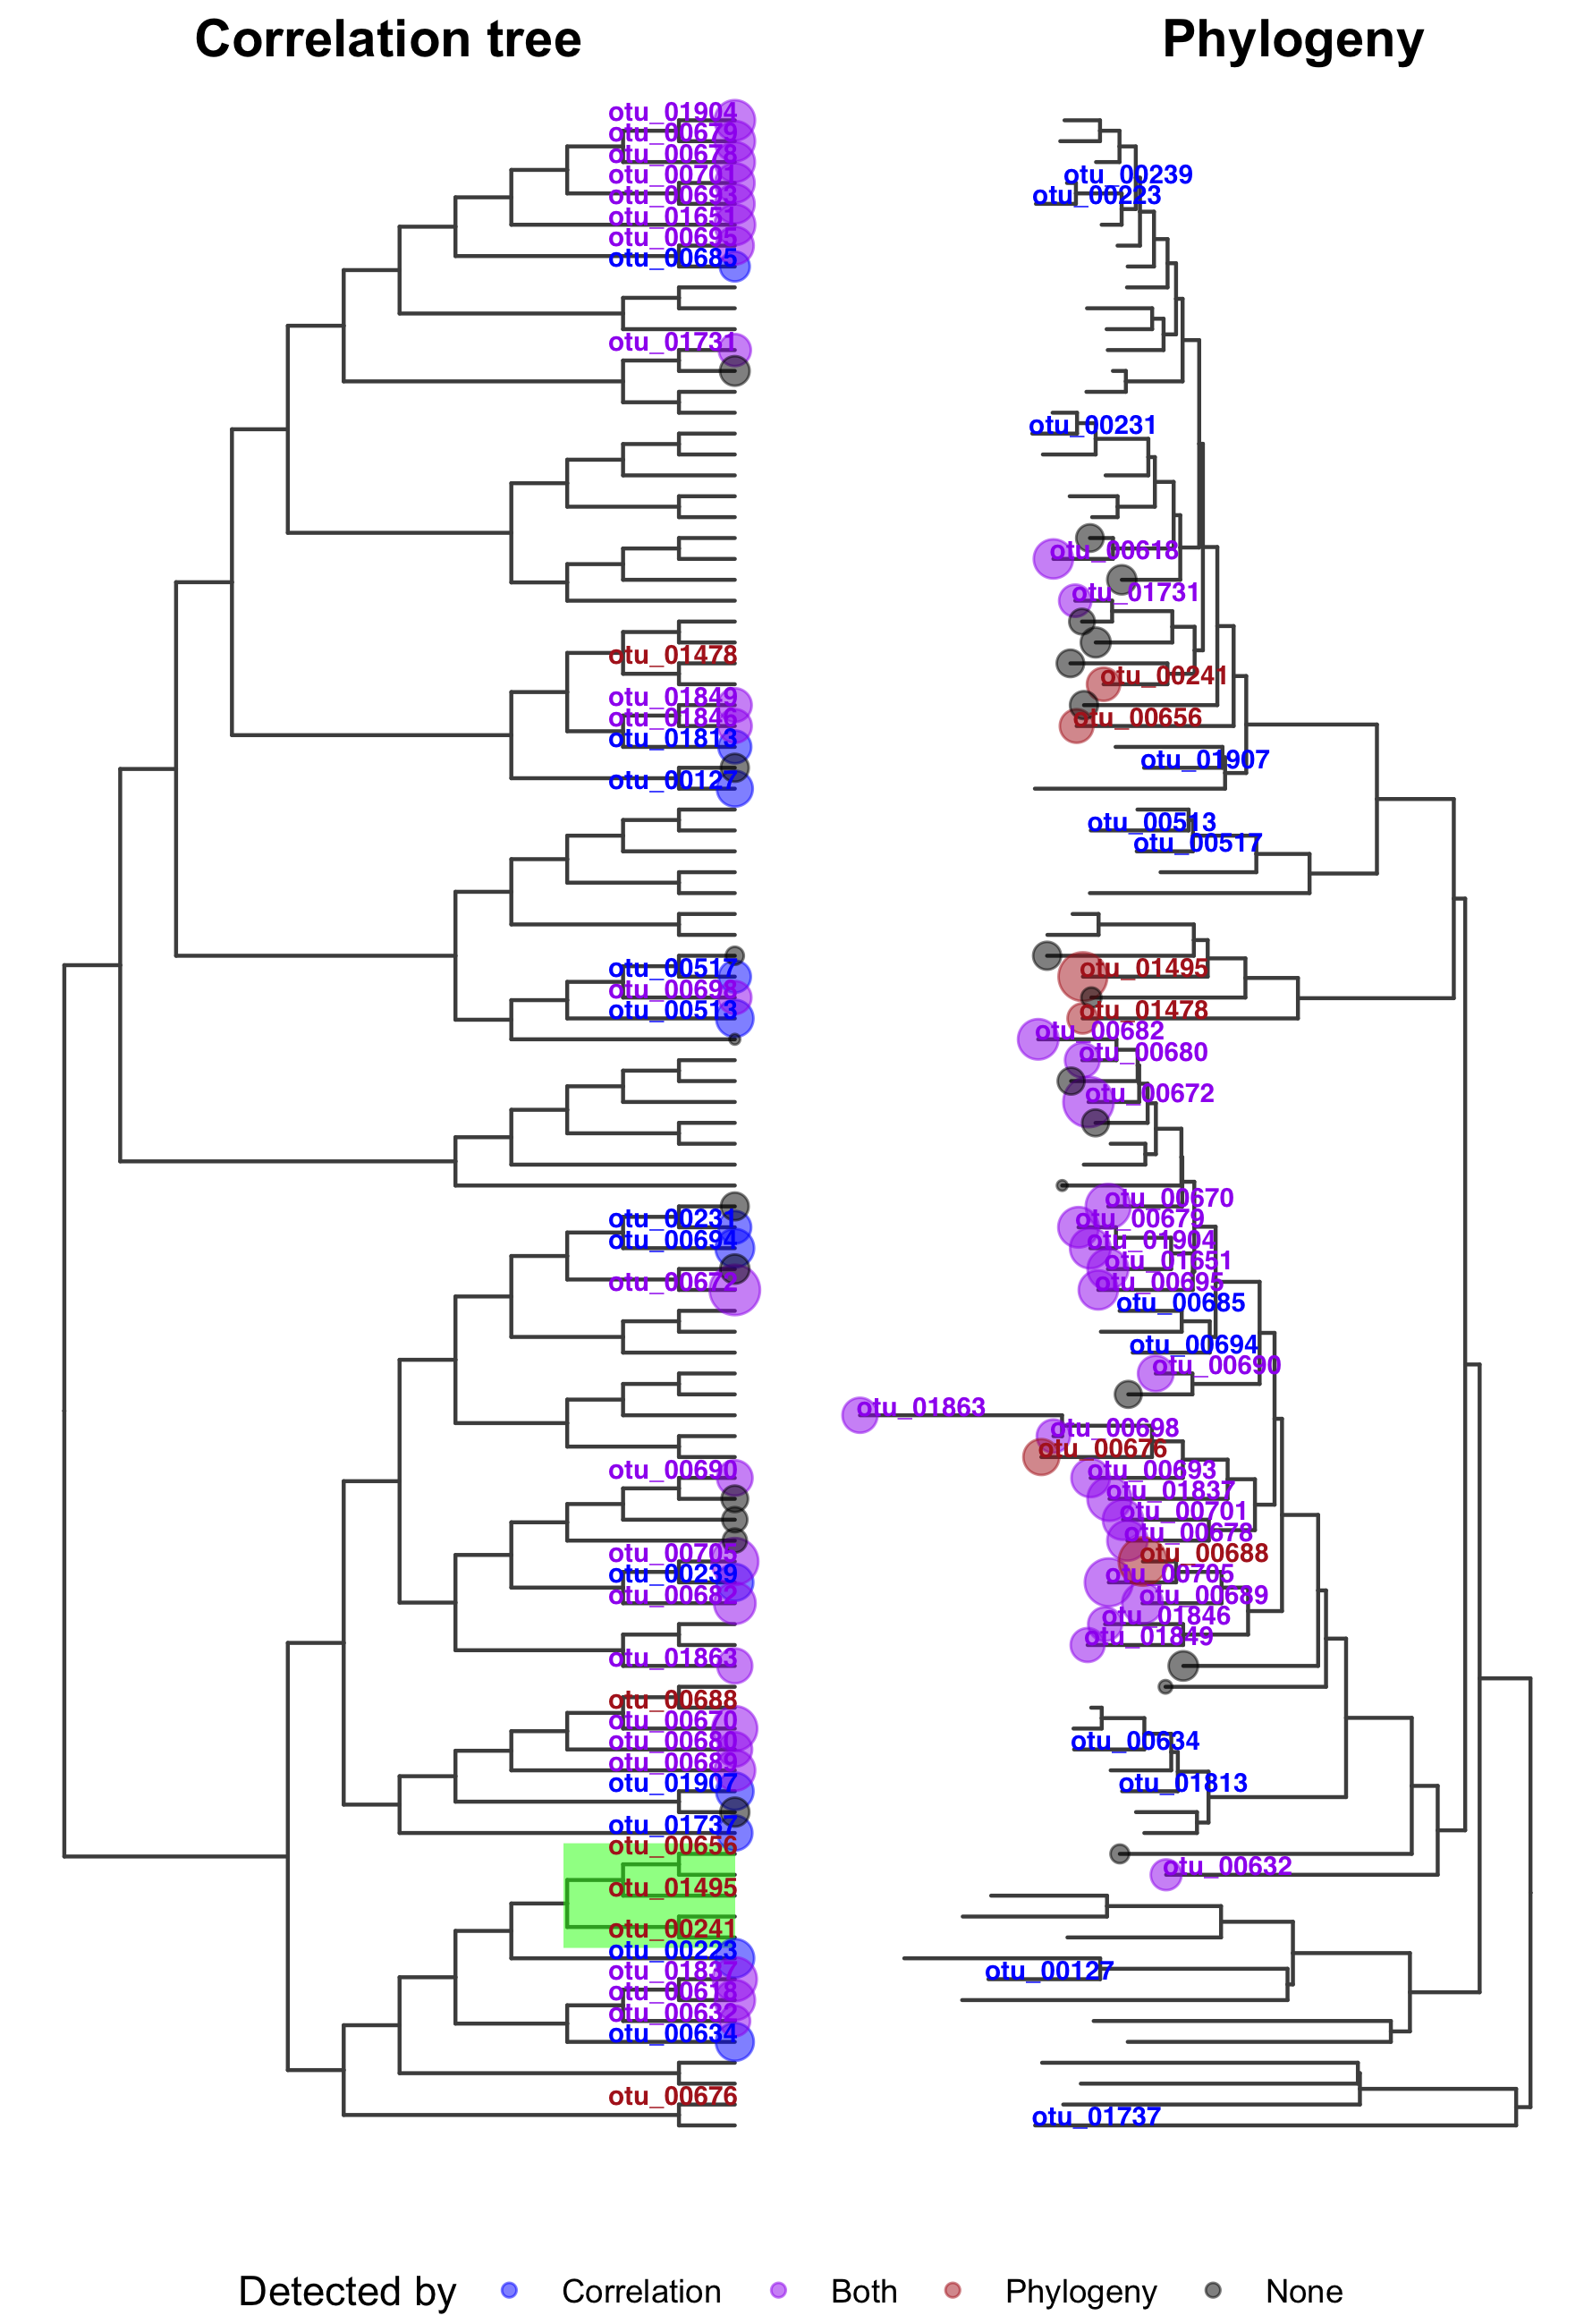
\includegraphics[width=0.9\linewidth]{img/chaillou_trees} 

}

\caption{Évidences des OTUs détectées avec l'arbre des corrélations (à droite) ou la phylogénie (à gauche).}\label{fig:chailloutrees}
\end{figure}
Si l'on regarde plus attentivement les cinq OTUs du cadre vert de la figure \ref{fig:chailloutrees}, on a trois OTUs qui ont été détectées uniquement par la phylogénie et non par l'arbre des corrélations alors qu'elles appartiennent au même clade de cinq individus dans celui-ci. La figure \ref{fig:chaillouzoom} met l'accent sur ces cinq OTUs, qui ne sont présentes quasiment que dans les crevettes. Le test de Fisher couplé au bruit causé par l'agrégation des données fait qu'on ne descend pas dans le sous-arbre en question. L'inaptitude de l'arbre des corrélations à identifier ces taxons est donc imputable à l'utilisation d'un test inadapté : remplacer le test de Fisher par un test non paramétrique de Kruskall-Wallis aurait permis à la procédure hiérarchique sur l'arbre des corrélations d'identifier l'ensemble des OTUs du clade.


\begin{figure}

{\centering 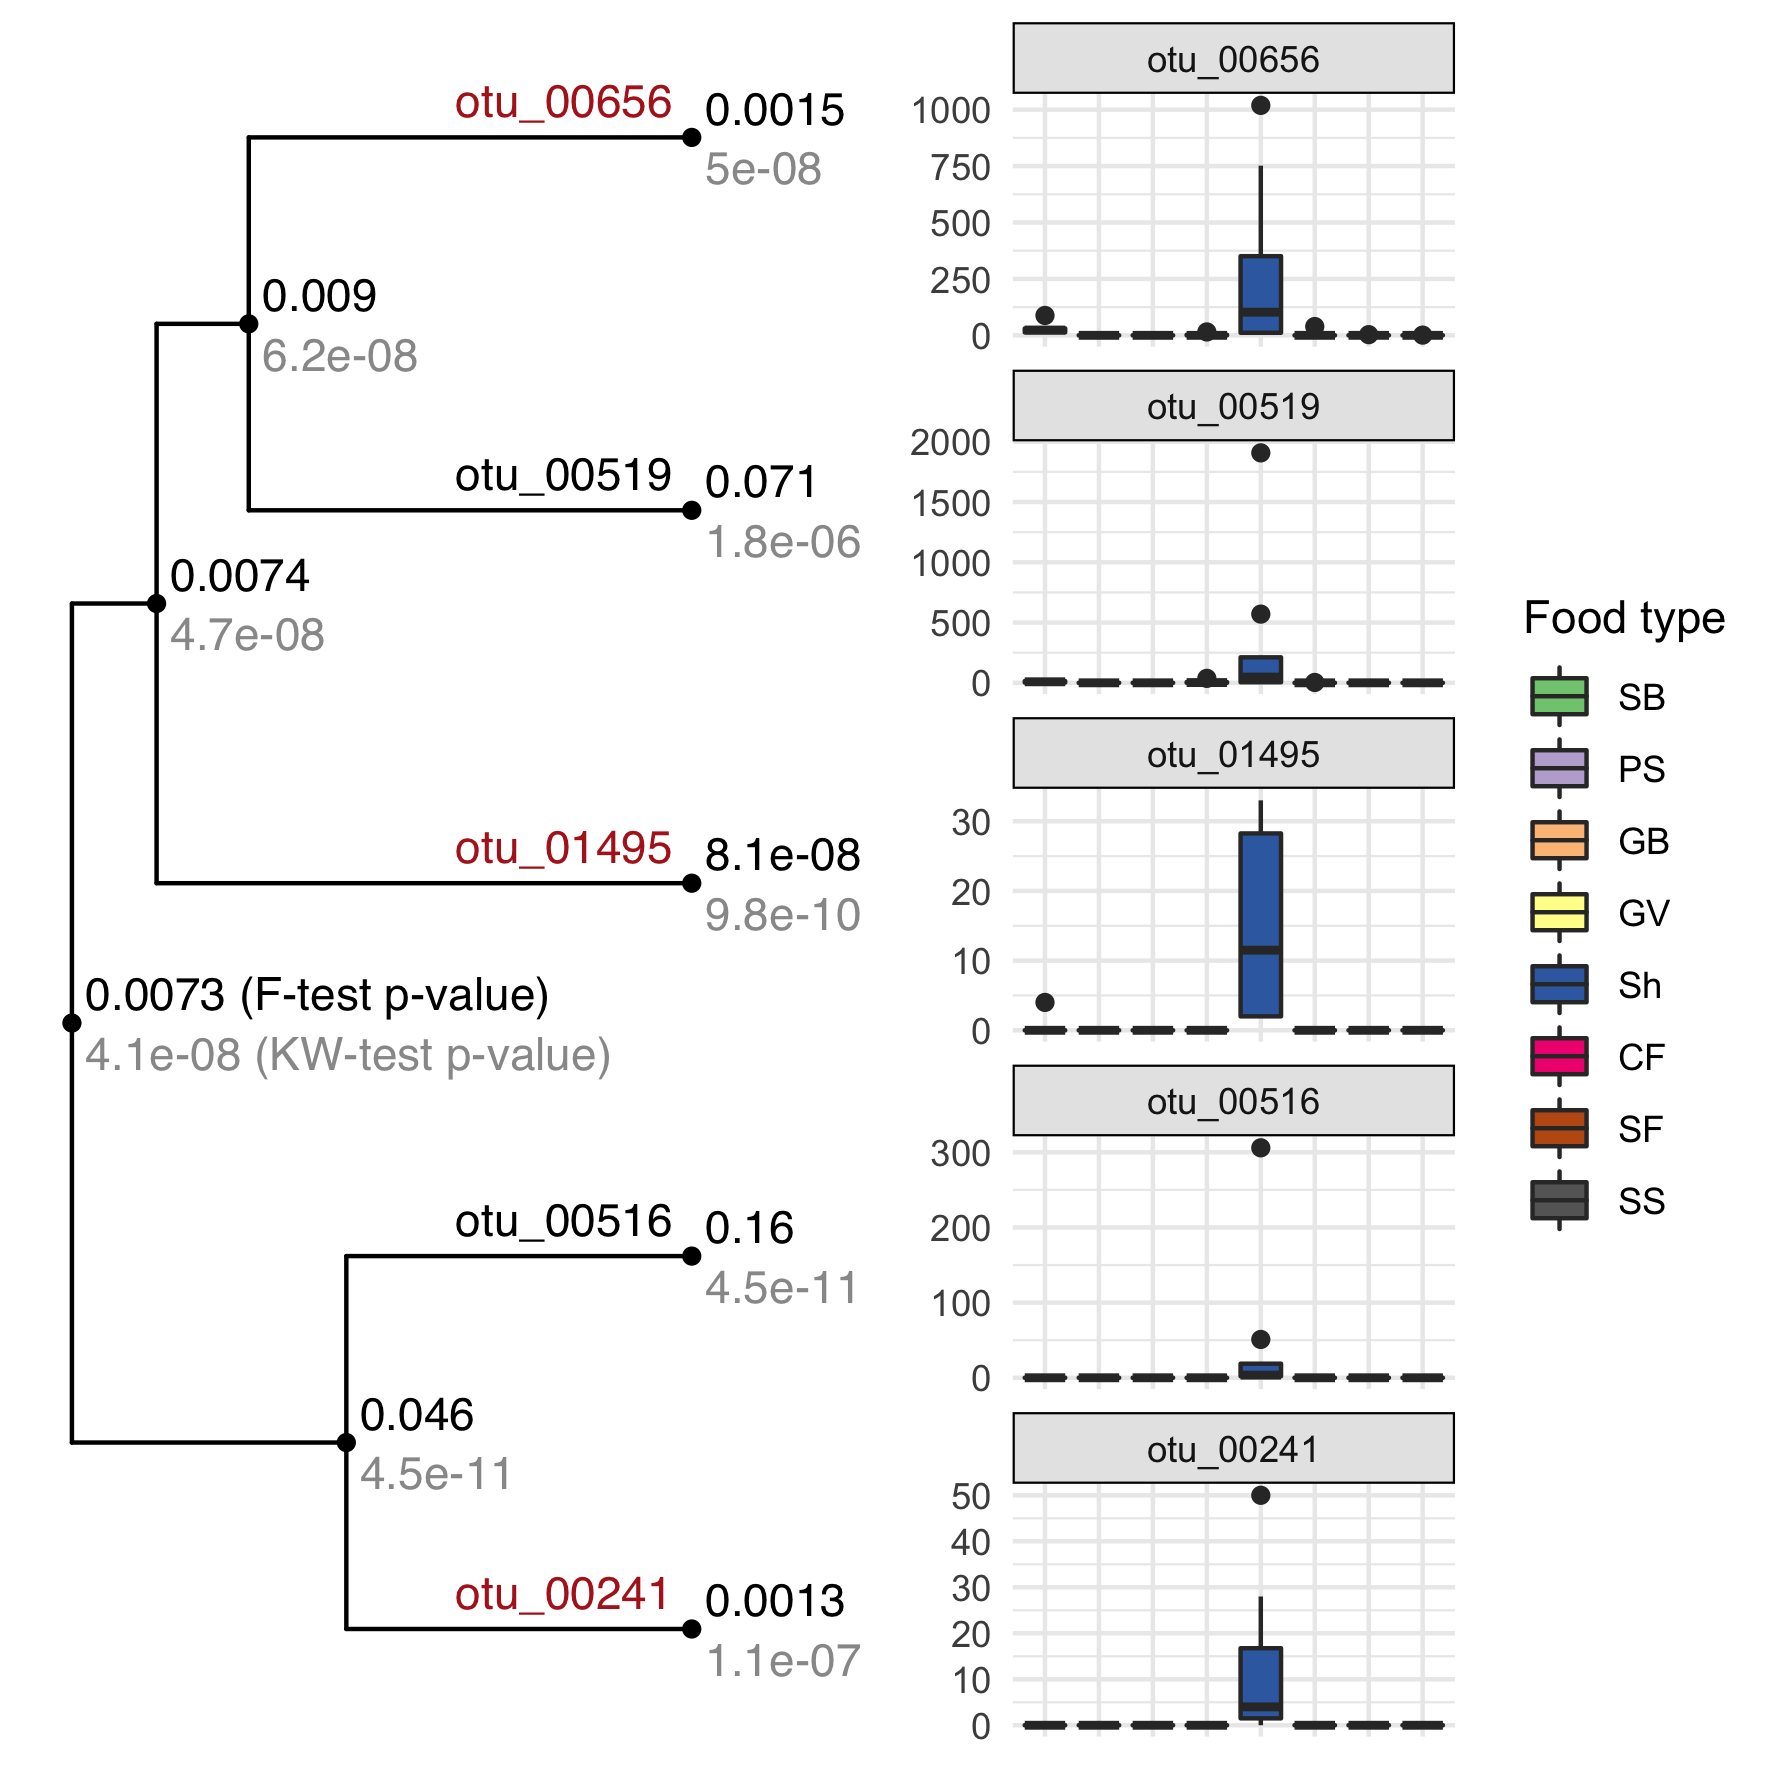
\includegraphics[width=0.9\linewidth]{img/chaillou_zoom} 

}

\caption{Focus sur les cinq OTUs du cadre vert de la figure \ref{fig:chailloutrees}.}\label{fig:chaillouzoom}
\end{figure}
\hypertarget{nouvelleapproche}{%
\chapter{\texorpdfstring{\emph{zazou} : une nouvelle approche}{zazou : une nouvelle approche}}\label{nouvelleapproche}}

\hypertarget{ou}{%
\section{Processus d'Ornstein-Uhlenbeck}\label{ou}}

Un processus d'Ornstein-Uhlenbeck (OU) de force de rappel \(\ou{\alpha}\), de valeur optimale \(\ou{\optim}\), et d'écart-type \(\ou{\sigma} > 0\) est un processus gaussien qui satisfait l'équation différentielle stochastique suivante :
\begin{equation*}
\dx{W_t} = - \ou{\alpha} (W_t - \ou{\optim}) \dx{t} + \ou{\sigma}\dx{B_t},
\end{equation*}
avec \(B\) le mouvement brownien unidimensionnel standard.

Si \(W_0\) est connu et fixé, l'espérance du processus vaut \(\EE{W_t} = W_0 e^{-\ou{\alpha} t} + \ou{\optim}\left(1 - e^{-\ou{\alpha} t}\right)\) et la covariance du processus est donnée par

\[\CC{W_t, W_s} = \frac{\ou{\sigma}^2}{2\ou{\alpha}}\left(e^{-\ou{\alpha} \left|t-s\right|} - e^{-\ou{\alpha} \left(t+s\right)}\right).\]

Le processus est gaussien et il admet pour loi limite \(\normal{\ou{\optim}}{\frac{\ou{\sigma}^2}{2\ou{\alpha}}}\), dont la variance est finie.

De par leurs propriétés, les processus d'Ornstein-Uhlenbeck sont devenus populaires pour modéliser l'évolution de traits biologiques continus, comme la masse corporelle des mammifères (Freckleton, Harvey, \& Pagel, \protect\hyperlink{ref-freckleton2003bergmann}{2003}).

Il est également possible de faire évoluer un processus d'Ornstein-Uhlenbeck sur un
arbre (Bastide, Mariadassou, \& Robin, \protect\hyperlink{ref-bastide2017detection}{2017}). Le long d'une branche, les paramètres du processus sont fixes. À chaque nœud, une branche se divise (en deux dans le cas d'un arbre binaire) et le processus donne naissance à deux copies indépendantes ayant la même valeur initiale au point de branchement. Cela induit notamment une dépendance statistique entre tous les descendants d'un même ancêtre. Cette dépendance est d'autant plus forte que l'ancêtre est récent. Sur la figure \ref{fig:treeou}, le processus vert partant de \(N_1\) jusqu'à \(N_2\) donne naissance à deux processus \(T_4\) et \(T_5\), jaune et bleu, lorsqu'il arrive au nœud \(N_2\).

De plus, à chaque branchement, un changement dans les paramètres du processus est susceptible de se produire. Dans ce cas, le processus garde la même valeur au nœud mais continue sa trajectoire avec les nouveaux paramètres. C'est le cas en \(N_3\) dans la figure \ref{fig:treeou} où le processus orange a subi un changement dans sa valeur optimale \(\ou{\optim}\) par rapport au processus rouge : la trajectoire est continue et le processus dérive vers la nouvelle valeur optimale.


\begin{figure}

{\centering 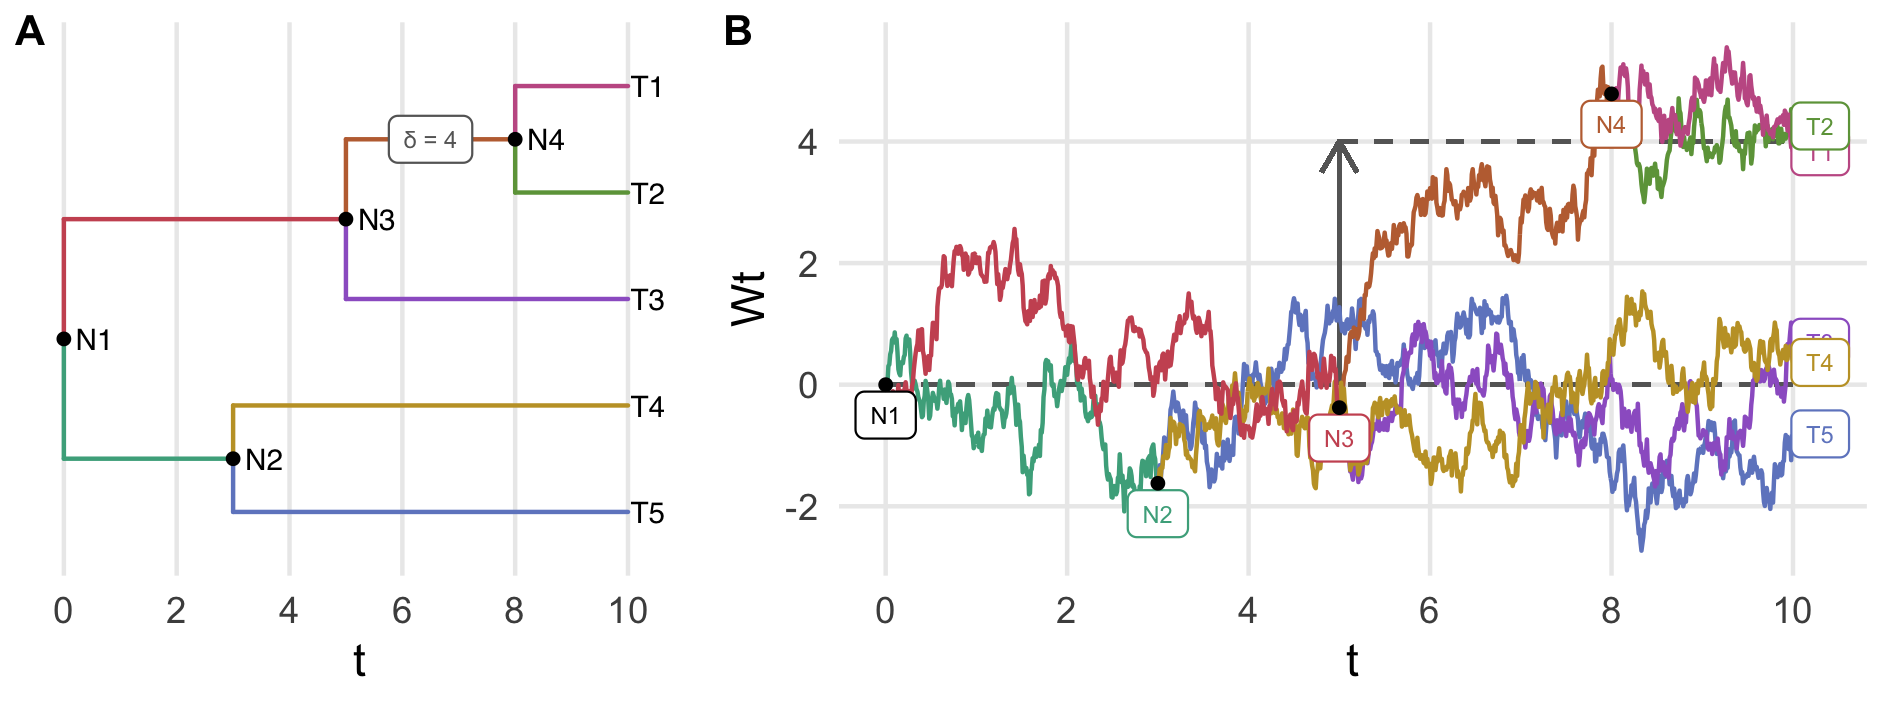
\includegraphics[width=0.9\linewidth]{img/tree_ou} 

}

\caption{Exemple d'un processus d'Ornstein-Uhlenbeck sur un arbre à 5 feuilles. À chaque branchement, le processus se scinde en deux processus indépendants ayant la même valeur initiale. Les paramètres sont conservés sauf lors d'un saut dans la valeur optimale, comme sur la branche conduisant à \(N_4\).}\label{fig:treeou}
\end{figure}
Le produit matriciel de la matrice d'incidence \(T\) par le vecteur de sauts \(\shifts\) permet d'effectuer la somme cumulée des sauts le long des branches pour obtenir la valeur optimale du processus aux feuilles. Dans l'exemple de la figure \ref{fig:treeou},
\begin{equation*}
\oui{\optim}{\{\text{feuilles}\}} = T \shifts = 
\begin{bmatrix}
1 & 0 & 0 & 0 & 0 & 1 & 0 & 1 & 1 \\
0 & 1 & 0 & 0 & 0 & 1 & 0 & 1 & 1 \\
0 & 0 & 1 & 0 & 0 & 1 & 0 & 1 & 0 \\
0 & 0 & 0 & 1 & 0 & 1 & 1 & 0 & 0 \\
0 & 0 & 0 & 0 & 1 & 1 & 1 & 0 & 0 \\
\end{bmatrix}
\cdot
\begin{bmatrix}
0 \\
0 \\
0 \\
0 \\
0 \\
0 \\
0 \\
0 \\
4 \\
\end{bmatrix} 
= 
\begin{bmatrix}
4 \\
4 \\
0 \\
0 \\
0 \\
\end{bmatrix}.
\end{equation*}
\newline

En notant \(\oui{\optim}{i}\) la valeur optimale du processus sur la branche descendant au nœud \(i\), la loi à ce nœud conditionnellement à son parent est
\begin{equation*}
X_i|X_{\text{pa}(i)} \sim \mathcal{N}\left( X_{\text{pa}(i)} e^{-\ou{\alpha} \ell_i } + \oui{\optim}{i} \left(1-e^{-\ou{\alpha} \ell_i}\right), \frac{\ou{\sigma}^2}{2\ou{\alpha}} \left(1 - e^{-2\ou{\alpha} \ell_i}\right) \right).
\end{equation*}
Ceci permet d'avoir une expression pour la covariance entre les nœuds \(i\) et \(j\). Dans le cas où \(P = \pa(i)=\pa(j)\), on a
\begin{equation*}
\begin{aligned}
\CC{X_i, X_j} & = \EE{X_iX_j} - \EE{X_i} \EE{X_j} \\
& = \EE{\EE{X_iX_j\mid P}} - \EE{\EE{X_i\mid P}} \EE{\EE{X_j \mid P }} \\
& = \EE{\left(P e^{-\ou{\alpha}\ell_i} + \oui{\optim}{i} \left(1-e^{-\ou{\alpha}\ell_i}\right)\right) \left(P e^{-\ou{\alpha}\ell_j} + \oui{\optim}{j} \left(1-e^{-\ou{\alpha}\ell_j}\right)\right)} \\
& \qquad - \EE{P e^{-\ou{\alpha}\ell_i} + \oui{\optim}{i} \left(1-e^{-\ou{\alpha}\ell_i}\right)} \EE{P e^{-\ou{\alpha}\ell_j} + \oui{\optim}{j} \left(1-e^{-\ou{\alpha}\ell_j}\right)} \\
& = e^{-\ou{\alpha}(\ell_i + \ell_j)} \EE{P^2} - e^{-\ou{\alpha}(\ell_i + \ell_j)} \EE{P}^2 \\
& = e^{-\ou{\alpha} d_{i,j}} \VV{P} \\
& = \frac{\ou{\sigma}^2}{2\ou{\alpha}}\left(1 - e^{-2\ou{\alpha} t_{i,j} }\right) \times e^{-\ou{\alpha} d_{i,j}}.
\end{aligned}
\end{equation*}
Cette expression reste valable quelque soit le niveau de parenté entre \(i\) et \(j\). Ainsi, pour un arbre ultramétrique de longueur \(h\), la matrice de variance-covariance du vecteur gaussien des feuilles (numérotées de 1 à \(m\)) est composée des éléments
\begin{equation}
\label{eq:covariance}
\frac{\ou{\sigma}^2}{2\ou{\alpha}}\left(e^{-\ou{\alpha} d_{i,j}} - e^{-2\ou{\alpha} h}\right).
\end{equation}
En particulier, la variance à toutes les feuilles est \(\frac{\ou{\sigma}^2}{2\ou{\alpha}}\left(1 - e^{-2\ou{\alpha} h}\right)\).

\hypertarget{zazousection}{%
\section{Zazou}\label{zazousection}}

\hypertarget{moduxe8le}{%
\subsection{Modèle}\label{moduxe8le}}

L'approche que nous avons développée s'appuie sur les \(z\)-scores aux feuilles et fait deux hypothèses :
\begin{enumerate}
\def\labelenumi{\arabic{enumi}.}
\tightlist
\item
  les \(z\)-scores sont la réalisation d'un processus d'Ornstein-Uhlenbeck avec sauts sur l'arbre phylogénétique,
\item
  sous \(\mathcal{H}_1\), \(\zs_i \sim \normal{\mu_i}{1}\) avec \(\mu_i < 0\).
\end{enumerate}
La première hypothèse nous permet de définir la distribution jointe des \(z\)-scores comme
\begin{equation*}
\zs \sim \mathcal{N}_{m}\left(\mu,\Sigma\right)
\end{equation*}
où \(\mu\) dépend de \(\shifts\), le vecteur des sauts du processus, via la relation \(\mu = T\delta\) et \(\Sigma\) dépend de \(\ou{\alpha}\) et \(\ou{\sigma}\) via l'équation \eqref{eq:covariance}.

La seconde hypothèse est classique lorsqu'on travaille sur les \(z\)-scores (McLachlan \& Peel, \protect\hyperlink{ref-mclachlan2004finite}{2004}) et est justifiée par le décalage à gauche des \(p\)-valeurs sous \(\mathcal{H}_1\) : \(\pv_i \preccurlyeq \unif{\mathopen[0, 1\mathclose]}\). Cette hypothèse implique alors l'équivalence entre trouver les hypothèses alternatives et déterminer les composantes non-nulles du vecteur \(\mu\). Sous \(\mathcal{H}_0\) et \(\mathcal{H}_1\), la variance aux feuilles doit valoir \(1\), ce qui impose
\begin{equation*}
\ou{\sigma}=\frac{2\ou{\alpha}}{1 - e^{-2\ou{\alpha}h}},
\end{equation*}
de sorte que \(\Sigma\) dépend uniquement de \(\ou{\alpha}\).

À ce stade, nous n'avons accès qu'au vecteur \(\zs\).

\hypertarget{estimation-ponctuelle}{%
\subsection{Estimation ponctuelle}\label{estimation-ponctuelle}}

En supposant \(\ou{\alpha}\) (et donc \(\Sigma\)) connue, une application naïve du maximum de vraisemblance donnerait
\begin{equation*}
\hat{\mu} = \argmin_{\mu\in\mathbb{R}_-^m} \|\zs - \mu\|_{\Sigma^{-1}, 2}^2
\end{equation*}
comme estimateur de \(\mu\). En réalité, c'est la position des sauts qui nous intéresse et nous souhaitons donc plutôt avoir un estimateur de \(\shifts\). En utilisant la relation \(\mu = T\shifts\), celui-ci est donné par
\begin{equation*}
\hat{\delta} = \argmin_{\shifts \in \shiftset} \left\|\zs - T\shifts\right\|_{\Sigma^{-1},2}^2,
\end{equation*}
où \(\shiftset = \left\{\shifts\in \mathbb{R}^{n} / T\shifts \in\mathbb{R}_-^m\right\}\) est l'ensemble de faisabilité pour les sauts qui induisent des composantes négatives aux feuilles. Bien que le problème soit convexe (la fonction objective est convexe, tout comme l'ensemble de faisabilité), la matrice \(T\) n'est pas de plein rang et l'estimateur \(\hat{\mu}\) n'est donc pas unique.

Nous lui préférons donc un estimateur parcimonieux, obtenu en rajoutant une contrainte \(\ell_1\) (Tibshirani, \protect\hyperlink{ref-tibshirani1996regression}{1996}) à la fonction objectif :
\begin{equation*}
\hat{\shifts} = \argmin_{\shifts \in \shiftset} \left\|\zs - T\shifts\right\|_{\Sigma^{-1},2}^2 + \lambda \|\shifts\|_1.
\end{equation*}
\newline

En utilisant la décomposition de Cholesky \(\Sigma^{-1} = R^TR\), ce nouveau problème peut se ramener au problème bien connu du lasso, avec une contrainte convexe sur \(\shifts\) :
\begin{equation}
\label{eq:lasso}
\hat{\shifts} = \argmin_{\shifts \in \shiftset} \left\|y - X\shifts\right\|_2^2 + \lambda \|\shifts\|_1,
\end{equation}
où \(y = R\zs \in \RR^m\) et \(X = RT \in \RR^{m \times n}\).

Le problème \eqref{eq:lasso} est convexe en \(\shifts\) et sa résolution est possible avec l'algorithme détaillé dans la section \ref{shooting}, qui est une modification de l'algorithme du \emph{shooting} (Fu, \protect\hyperlink{ref-fu1998penalized}{1998}).

Il reste maintenant à déterminer \(\ou{\alpha}\) et \(\lambda\). Ceux-ci ne pouvant être obtenus directement à partir des données, nous allons sélectionner le couple qui minimise le critère BIC suivant :
\begin{equation*}
\left(\ou{\hat{\alpha}}, \hat{\lambda}\right) = \argmin_{\alpha > 0, \lambda \geq 0} \left\|\zs - T\shifts_{\alpha, \lambda}\right\|_{\Sigma(\alpha)^{-1},2}^2 + \log|\Sigma(\alpha)| + \|\shifts_{\alpha, \lambda}\|_0 \log{m},
\end{equation*}
où \(\shifts_{\alpha, \lambda}\) est la solution du problème \eqref{eq:lasso} pour \(\alpha\) et \(\lambda\). En pratique, une grille bidimensionnelle donne les valeurs du couple à tester. Cette approche a été préférée à l'alternative usuelle de la validation croisée pour ne pas avoir à gérer la dépendance entre les \(z\)-scores.

\hypertarget{duxe9biaisage-et-intervalles-de-confiance}{%
\subsection{Débiaisage et intervalles de confiance}\label{duxe9biaisage-et-intervalles-de-confiance}}

L'estimateur lasso est connu pour être biaisé (Javanmard \& Montanari, \protect\hyperlink{ref-javanmard2013confidence}{2013}) et ne produit pas d'intervalles de confiance pour les \(\hat{\shifts}_i\). Nous utilisons donc une procédure de débiaisage, comme celles proposées dans Zhang \& Zhang (\protect\hyperlink{ref-zhang2014confidence}{2014}) ou Javanmard \& Montanari (\protect\hyperlink{ref-javanmard2013confidence}{2013}) et Javanmard \& Montanari (\protect\hyperlink{ref-javanmard2014confidence}{2014}). Ces deux procédures fonctionnent suivant le même principe. Tout d'abord, au lieu d'avoir un estimateur initial de \(\shifts\) comme dans \eqref{eq:lasso}, nous avons besoin d'un estimateur couplé de \(\shifts\) et de sa variance \(\sigma\), qui peut être obtenu par un \emph{scaled lasso} (Sun \& Zhang, \protect\hyperlink{ref-sun2012scaled}{2012}) et qui sera notre estimateur initial :
\begin{equation*}
\left(\hat{\shifts}^{\text{(init)}},\ \hat{\sigma}\right) = \argmin_{\shifts \in \shiftset, \sigma > 0}  \frac{\|y - X \shifts\|_2^2}{2\sigma m} + \frac{\sigma}{2} + \lambda \|\shifts\|_1.
\end{equation*}
\newline

L'estimation jointe est faite de façon itérative en alternant des étapes de mise à jour de
\(\hat{\shifts}^{\text{(init)}}\) par lasso et de mise à jour de \(\hat{\sigma}\) par résolution exacte, via l'expression \(\hat{\sigma} = \frac{\left\|y - X \hat{\shifts}^{\text{(init)}}\right\|_2}{\sqrt{m}}\). Une fois cette estimation initiale obtenue, Zhang \& Zhang (\protect\hyperlink{ref-zhang2014confidence}{2014}) proposent de calculer un système de score \(S\), qu'on peut comprendre comme une orthogonalisation faible de \(X\), pour corriger \(\hat{\shifts}^{\text{(init)}}\). La colonne \(s_j\) de \(S\) s'obtient comme étant le résidu de la régression lasso de \(x_j\) contre \(X_{-j}\), le reste des colonnes de \(X\).

Puis, l'estimateur débiaisé s'obtient alors en en corrigeant \(\hat{\shifts}_j^{\text{(init)}}\) comme suit :
\begin{equation*}
\hat{\shifts}_j = \hat{\shifts}_j^{\text{(init)}} + \frac{\langle s_j,y-X\hat{\shifts}^{(\text{init})}\rangle}{\langle s_j,x_j\rangle}.
\end{equation*}
\newline

Javanmard \& Montanari (\protect\hyperlink{ref-javanmard2013confidence}{2013}) et Javanmard \& Montanari (\protect\hyperlink{ref-javanmard2014confidence}{2014}) proposent une correction alternative
\begin{equation*}
\hat{\shifts} = \hat{\shifts}^{(\text{init})} + \frac{1}{m}SX^T \left(Y-X\hat{\shifts}^{(\text{init})}\right),
\end{equation*}
basée sur un système de score différent. La matrice \(S\) est cette fois-ci un inverse généralisé de \(M = \frac{X^TX}{m}\), construit colonne par colonne en résolvant les problèmes suivants :
\begin{equation*}
\left\{
  \begin{aligned}
    s_j & = \argmin_{s \in \mathbb{R}^{n}} \ s^TMs \\
    &\text{t.q.}\  \|Ms - e_j\|_{\infty} \leq \gamma
  \end{aligned}
\right.
\end{equation*}
où \(e_j \in \RR^n\) est le \(j^{\text{ème}}\) vecteur de la base canonique définie par \(e_{ij} = \delta_{i,j}\). Dans chacune des deux méthodes, sous des hypothèses standard en régression en grande dimension, \(\hat{\shifts}\sim \mathcal{N}_n\left(\shifts,V\right)\) ce qui permet d'obtenir un intervalle de confiance bilatéral au niveau \(\alpha\) pour \(\shifts_j\) :
\begin{equation*}
\left[ \hat{\shifts}_j \pm \phi^{-1}\left(1-\frac{\alpha}{2}\right) \sqrt{v_{j,j}} \right].
\end{equation*}
\newline

Avec le premier système de score, \(V\) se calcule élément par élément :
\begin{equation*}
v_{i,j} = \hat{\sigma}^2 \frac{\langle s_i,s_j\rangle}{\langle s_i,x_i\rangle\langle s_j,x_j\rangle},
\end{equation*}
tandis qu'avec le second, \(V = \frac{S M S^T }{m}\). En exprimant la \(i^{\text{ème}}\) composante de \(\mu\) à l'aide de \(\optim\) comme étant \(\mu_i = t_{i.}^T\shifts\) où \(t_{i.}\) est la \(i^{\text{ème}}\) ligne de \(T\), on obtient également un intervalle de confiance unilatéral au niveau \(\alpha\) pour \(\hat{\mu}_i\) :
\begin{equation*}
\left[-\infty, \hat{\mu}_i + \sqrt{t_{i.}^T V t_{i.}} \phi^{-1}\left(1-\alpha\right)\right],
\end{equation*}
et la \(p\)-valeur associée à cet intervalle, qui teste \(\mathcal{H}_0 = \left\{\mu_i = 0\right\}\) contre \(\mathcal{H}_1 = \left\{\mu_i < 0\right\}\), est donc
\begin{equation*}
\pv^\text{h}_i = \Phi\left(\frac{t_{i.}^T\hat{\shifts}}{\left(t_{i.}^TVt_{i.}\right)^{1/2}}\right),
\end{equation*}
qui est la \(p\)-valeur lissée hiérarchiquement.

\hypertarget{correction-pour-tests-multiples}{%
\subsection{Correction pour tests multiples}\label{correction-pour-tests-multiples}}

Une fois ces \(p\)-valeurs lissées obtenues, Javanmard, Javadi, \& others (\protect\hyperlink{ref-javanmard2019false}{2019}) proposent une méthode de correction pour tests multiples conçue spécialement pour le lasso débiaisé et qui repose sur les \(t\)-scores
\(\ts_i = \frac{t_{i.}^T\hat{\shifts}}{\left(t_{i.}^TVt_{i.}\right)^{1/2}}\).

Définissons \(t_{\text{max}} = \sqrt{2 \log m - 2 \log \log m}\) puis
\begin{equation}
\label{eq:tstar}
t^{\star} = \inf \bigg\{ 0 \leq t \leq t_{\max} : \underbrace{\frac{2m(1 - \Phi(t))}{R(t) \vee 1}}_{\widehat{\text{FDR}}(t)} \leq \alpha \bigg\},
\end{equation}
où \(R(t)= \sum_{i = 1}^m \indic_{\{\ts_i \leq -t\}}\) est le nombre d'hypothèses nulles rejetées au niveau \(t\). Le numérateur du quotient peut s'interpréter comme le nombre attendu de rejets sous l'hypothèse nulle, et celui-ci est donc une estimation du \(\text{FDR}\) au niveau \(t\), que l'on cherche à garder sous le seuil \(\alpha\). Si l'infimum en \eqref{eq:tstar} est \(+\infty\), on pose \(t^{\star} = \sqrt{2 \log m}\).

On rejette \(\mathcal{H}_0\) si \(\ts_i \leq -t^{\star}\) ce qui amène à définir les \(q\)-valeurs hiérarchiques
\begin{equation*}
\qv^{\text{h}}_i = \frac{\pv^{\text{h}}_i \alpha}{\Phi(-t^{\star})},
\end{equation*}
et l'hypothèse nulle associée est rejetée si \(\qv^{\text{h}}_i < \alpha\). Cette procédure contrôle le FDR au niveau \(\alpha\) (Javanmard et al., \protect\hyperlink{ref-javanmard2019false}{2019}).
\begin{remark}
\iffalse{} {Remarque. } \fi{}Comme \(t^{\star}\) dépend de \(\alpha\), les \(q\)-valeurs dépendent aussi de \(\alpha\) et doivent être calculées pour chaque niveau de FDR cible, contrairement à la procédure BH(\(\alpha\)) standard.
\end{remark}
\hypertarget{evaluation}{%
\section{Évaluation de la méthode}\label{evaluation}}

\hypertarget{simuzazou}{%
\subsection{Données simulées}\label{simuzazou}}

Afin d'évaluer la qualité de notre procédure, nous avons simulé des données de manière non-paramétrique, comme présenté dans la section \ref{checktreefdr} et dans la figure \ref{fig:abdiff} : à partir d'un jeu de données homogènes, on sélectionne des taxons différentiellement abondants, on assigne un groupe \(A\) ou \(B\) à chacun des échantillon et on multiplie les abondances de chaque taxon différentiellement abondant dans le groupe \(B\) par un \emph{fold-change} prédéterminé.

Trois déclinaisons de simulations ont été adoptées. Dans la première, dite positive, les taxons sont sélectionnés pour former des groupes dans la phylogénie et un \emph{fold-change} de \(3\), \(5\) ou \(10\) est ensuite appliqué. Ceci permet de créer des simulations pour lesquelles l'arbre est réellement informatif. Plus précisément, pour sélectionner les taxons différentiellement abondants, on applique un algorithme des \(k\)-médoïdes (Reynolds, Richards, Iglesia, \& Rayward-Smith, \protect\hyperlink{ref-reynolds2006clustering}{2006}) à la matrice des distances patristiques (Sneath, Sokal, \& others, \protect\hyperlink{ref-sneath1973numerical}{1973}), ce qui donne des groupes de taxons à faible distance patristique les uns des autres, qui correspondent généralement à un sous-arbre de la phylogénie. Un ou plusieurs groupes sont alors sélectionnés aléatoirement et leurs taxons sont déclarés différentiellement abondants.

Les deux autres déclinaisons de la procédure de simulation de jeux de données sont dites négatives. Pour l'une, les taxons sont sélectionnés uniformément dans l'arbre puis un \emph{fold-change} de \(5\) est appliqué, pour créer des simulations dans lesquelles le modèle est mal spécifié. Pour l'autre le \emph{fold-change} appliqué vaut \(1\), ce qui permet de voir comment réagit l'algorithme lorsqu'aucun taxon n'est différentiellement abondant.

La figure \ref{fig:tprfdrzazou} présente les résultats dans le cas des simulations positives. Si les procédures de corrections classiques (BH et BY) contrôlent bien le FDR à \(5~\%\), ce n'est pas le cas pour les procédures hiérarchiques. Dans la majorité des cas, le FDR des procédures hiérarchiques reste en dessous de \(6~\%\) mais pour la procédure à système de score (ss) avec un \emph{fold-change} de \(5\) et pour celle avec l'inverse généralisé par colonne (ci) avec un \emph{fold-change} de \(3\), il passe à \(8\) et \(9~\%\) respectivement. Dans toutes les configurations, BY a le TPR le plus faible, BH et \emph{TreeFDR} (tf) se comportent de manière semblable, conformément aux résultats présentés dans Bichat et al. (\protect\hyperlink{ref-bichat2020incorporating}{2020}), et les deux variantes de \emph{zazou} obtiennent le meilleur TPR.


\begin{figure}

{\centering 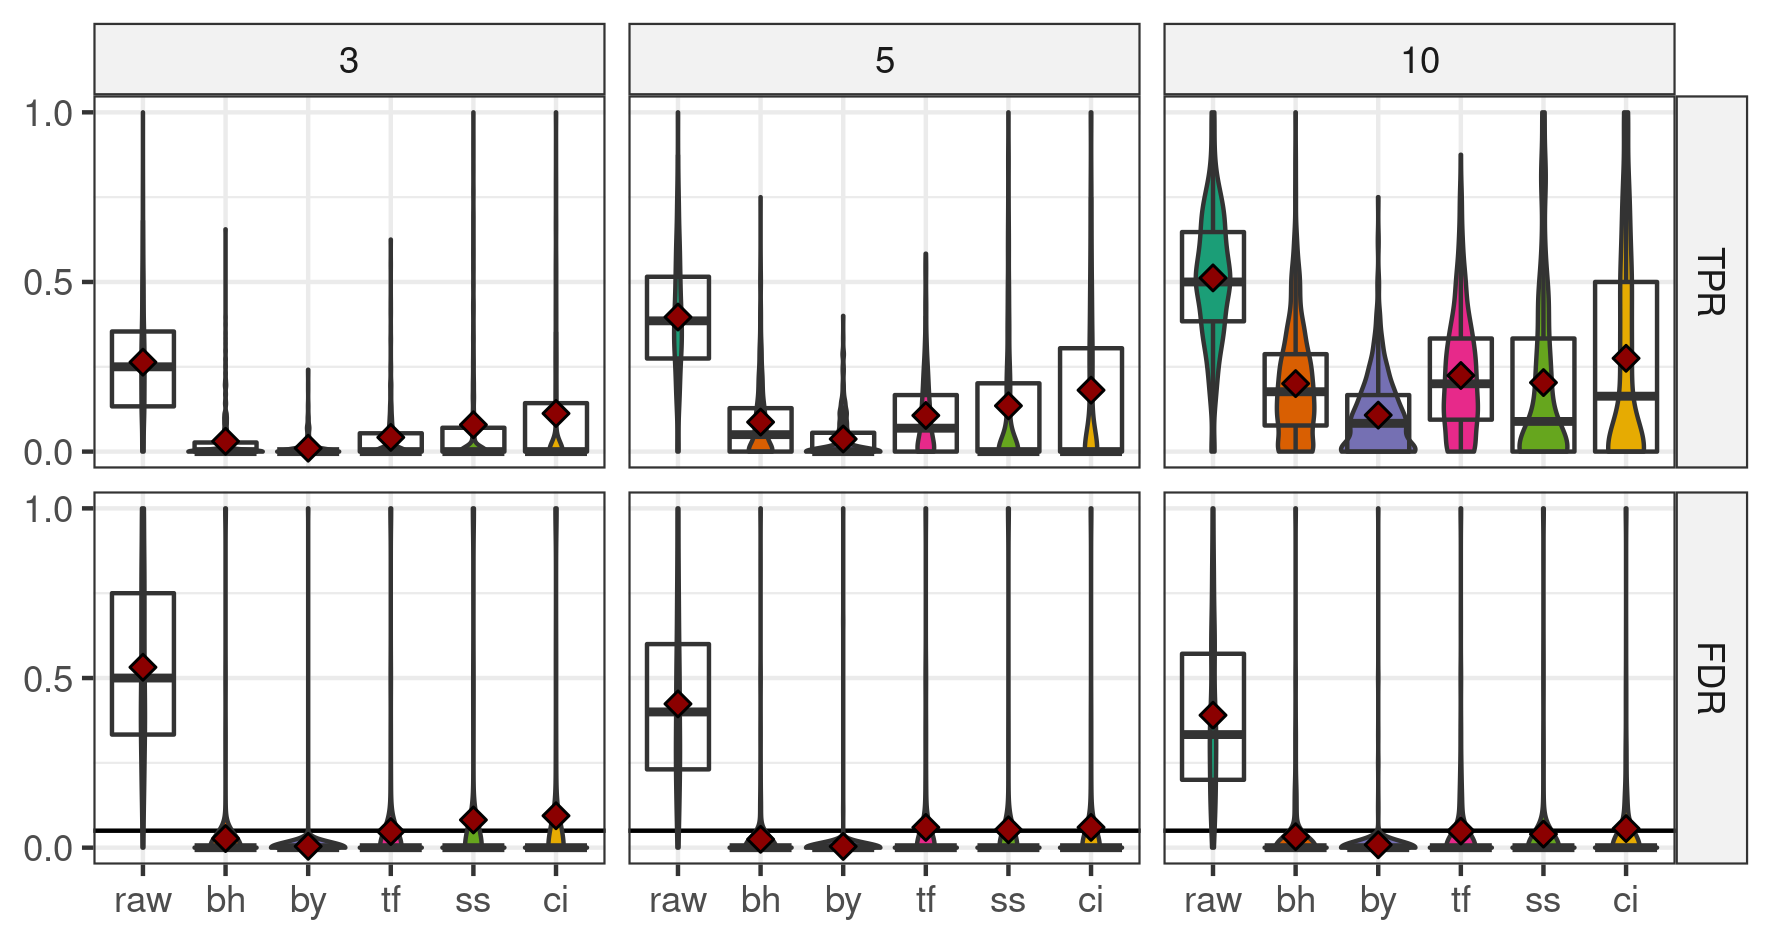
\includegraphics[width=0.9\linewidth]{img/tprfdr_zazou} 

}

\caption{TPR (haut) et FDR (bas) pour les différentes procédures et différents \emph{fold-changes} (en colonnes) dans le cadre des simulations positives.}\label{fig:tprfdrzazou}
\end{figure}
Le taux de faux positif plus élevé qu'attendu pour les résultats de \emph{zazou} suggère que le choix du seuil de détection proposé dans Javanmard et al. (\protect\hyperlink{ref-javanmard2019false}{2019}) n'est pas complètement adapté. Nous comparons donc les performances des différentes méthodes à l'aide de l'AUC, qui est une mesure indépendante du seuil. La figure \ref{fig:aucroczazou} met en évidence les meilleures performances de \emph{zazou}, dans ses deux variantes. En regardant la partie gauche des courbes ROC, on s'aperçoit que \emph{zazou} est plus performant dès les premières découvertes et que cela n'est pas un effet compensatoire des seuils plus élevés. Comme mentionné précédemment, BH et \emph{TreeFDR} obtiennent des performances similaires et moins bonnes que celles de \emph{zazou}. BY est la méthode la moins satisfaisante (du fait du grand nombre de \(p\)-valeurs ajustées à \(1\)).


\begin{figure}[!t]

{\centering 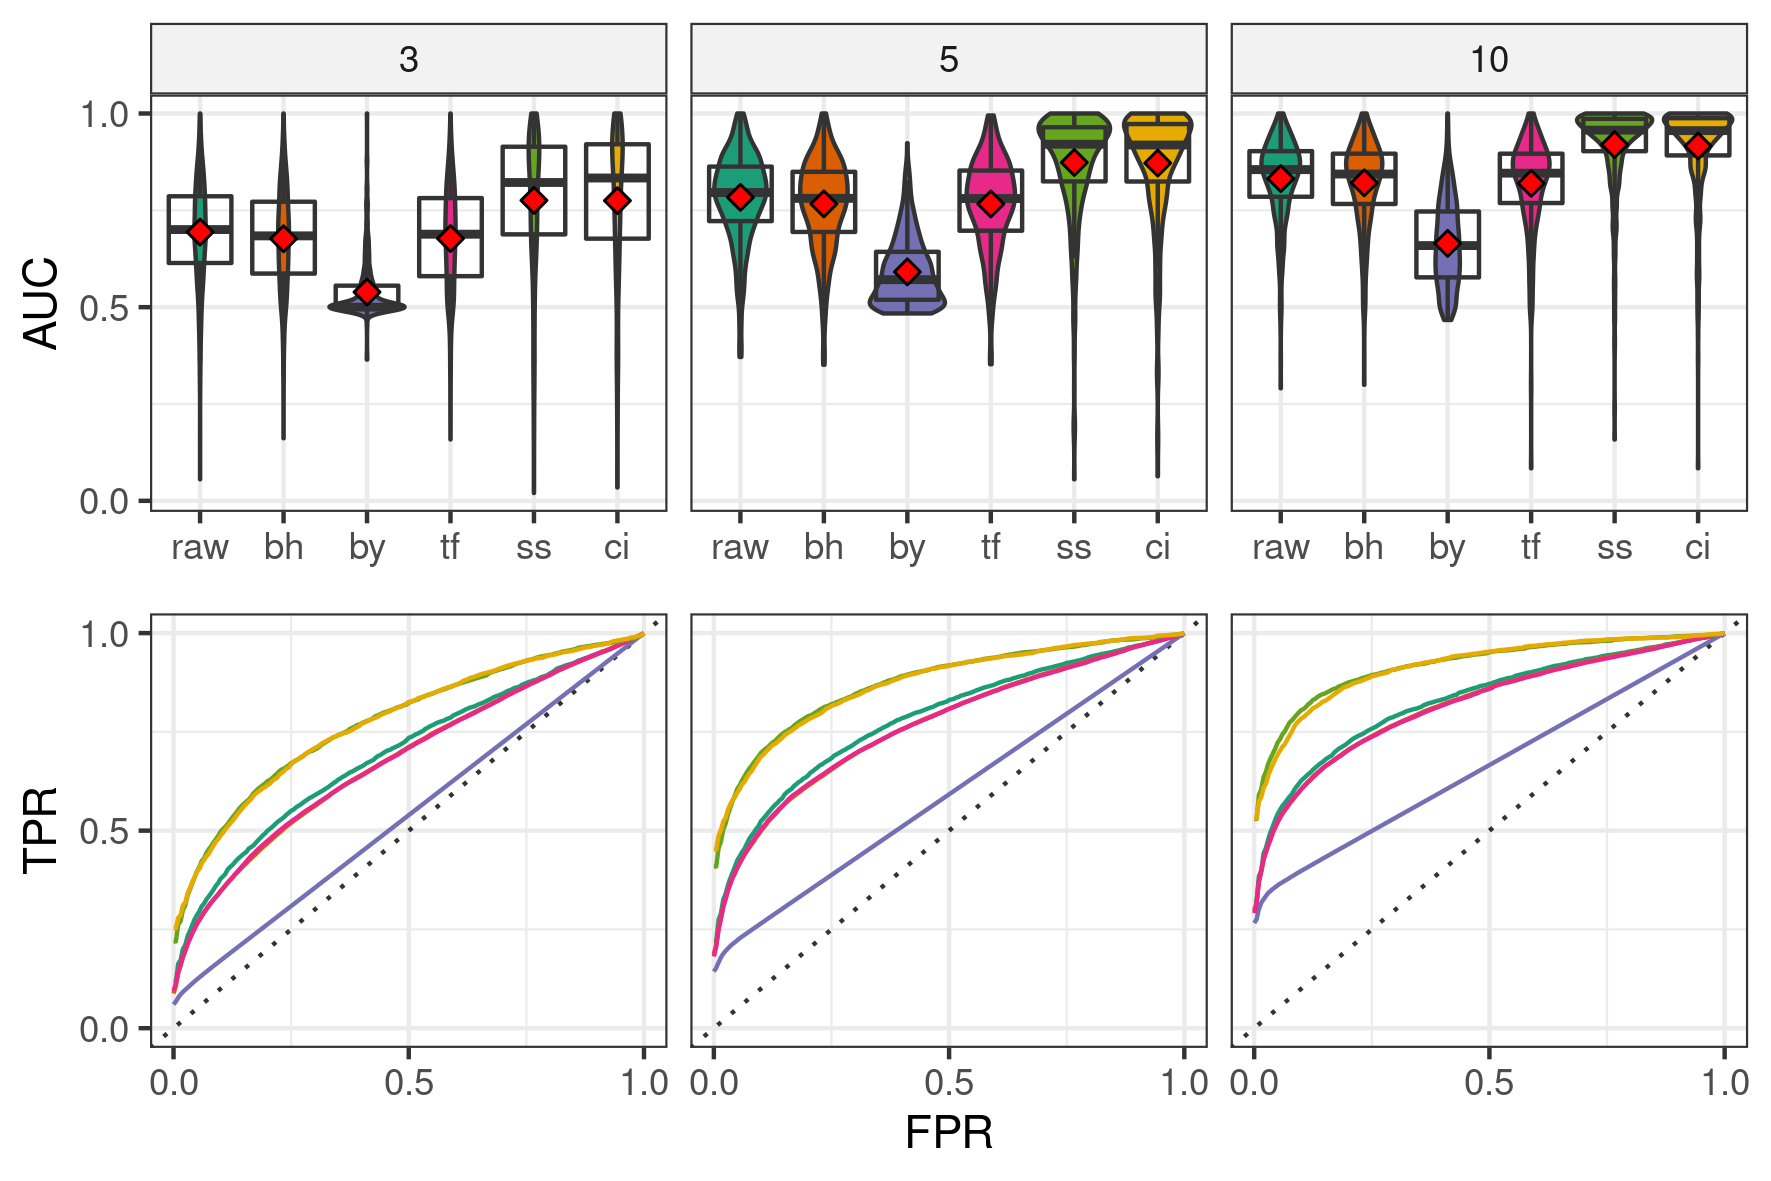
\includegraphics[width=0.9\linewidth]{img/aucroc_zazou} 

}

\caption{Distribution des AUC (haut) et courbes ROC (bas) pour les différentes procédures et \emph{fold-changes} (en colonnes) dans le cadre des simulations positives.}\label{fig:aucroczazou}
\end{figure}
Dans le cas des simulations négatives (figure \ref{fig:aucnegzazou}), l'imposition d'une contrainte hiérarchique inadaptée fait perdre \(15\) à \(20\) points d'AUC à \emph{zazou} par rapport à BH. Ce phénomène ne se retrouve pas dans les résultats de \emph{TreeFDR}, qui est pourtant également une procédure hiérarchique, grâce à une astuce d'implémentation. En effet, \emph{TreeFDR} effectue une correction de BH en parallèle de la procédure de lissage, et si cette dernière détecte bien moins de taxons que BH, les résultats de BH sont renvoyés à la place de ceux obtenus par lissage (Bichat et al., \protect\hyperlink{ref-bichat2020incorporating}{2020}; Xiao et al., \protect\hyperlink{ref-xiao2017false}{2017}).


\begin{figure}[!t]

{\centering 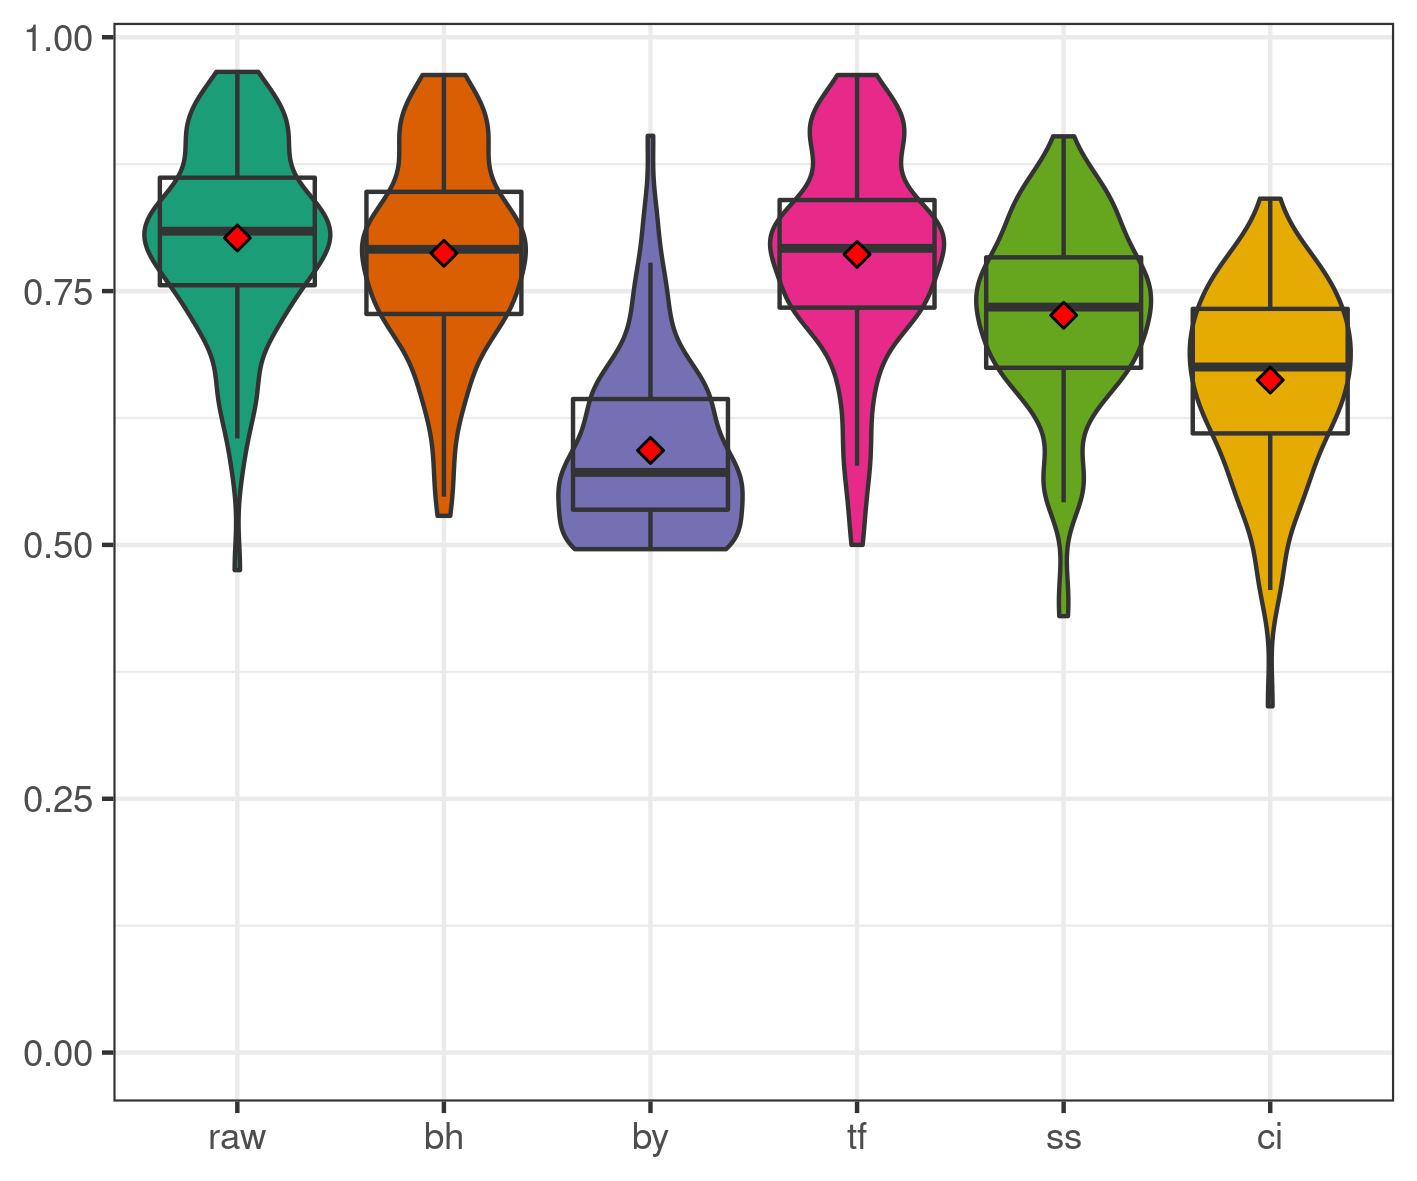
\includegraphics[width=0.4\linewidth]{img/aucneg_zazou} 

}

\caption{Distribution des AUC pour les différentes procédures lorsque les taxons différentiellement abondants sont sélectionnés uniformément.}\label{fig:aucnegzazou}
\end{figure}
Enfin, pour les simulations où aucun taxon n'est différentiellement abondant (\(\text{fc} = 1\)), les procédures ne détectent aucun faux positif, comme attendu.

\hypertarget{influence-de-luxe2ge}{%
\subsection{Influence de l'âge}\label{influence-de-luxe2ge}}

Nous avons comparé l'effet des différentes procédures de correction lors d'une analyse d'abondance différentielle entre des \(112\) adultes et \(34\) enfants au sein du jeu de données de Brito et al. (\protect\hyperlink{ref-brito2016mobile}{2016}) des populations insulaires. Des tests de Wilcoxon ont été effectués sur les 387 espèces présentes et 21 espèces ont été détectées à \(5~\%\) sans correction. Après correction par BH, BY, \emph{TreeFDR} ou \emph{treeclimbR}, aucune espèce n'est détectée. En revanche, \emph{zazou} en détecte certaines avec ses deux variantes : 17 pour ss et 6 pour ci.

La figure \ref{fig:heattree} montre que les espèces détectées par \emph{zazou} ne forment pas un sous-ensemble de celles obtenues sans correction. Au contraire, \emph{zazou} identifie des espèces proches de certaines détectées sans correction, majoritairement dans la zone mise en évidence par le bandeau rouge.


\begin{figure}[!t]

{\centering 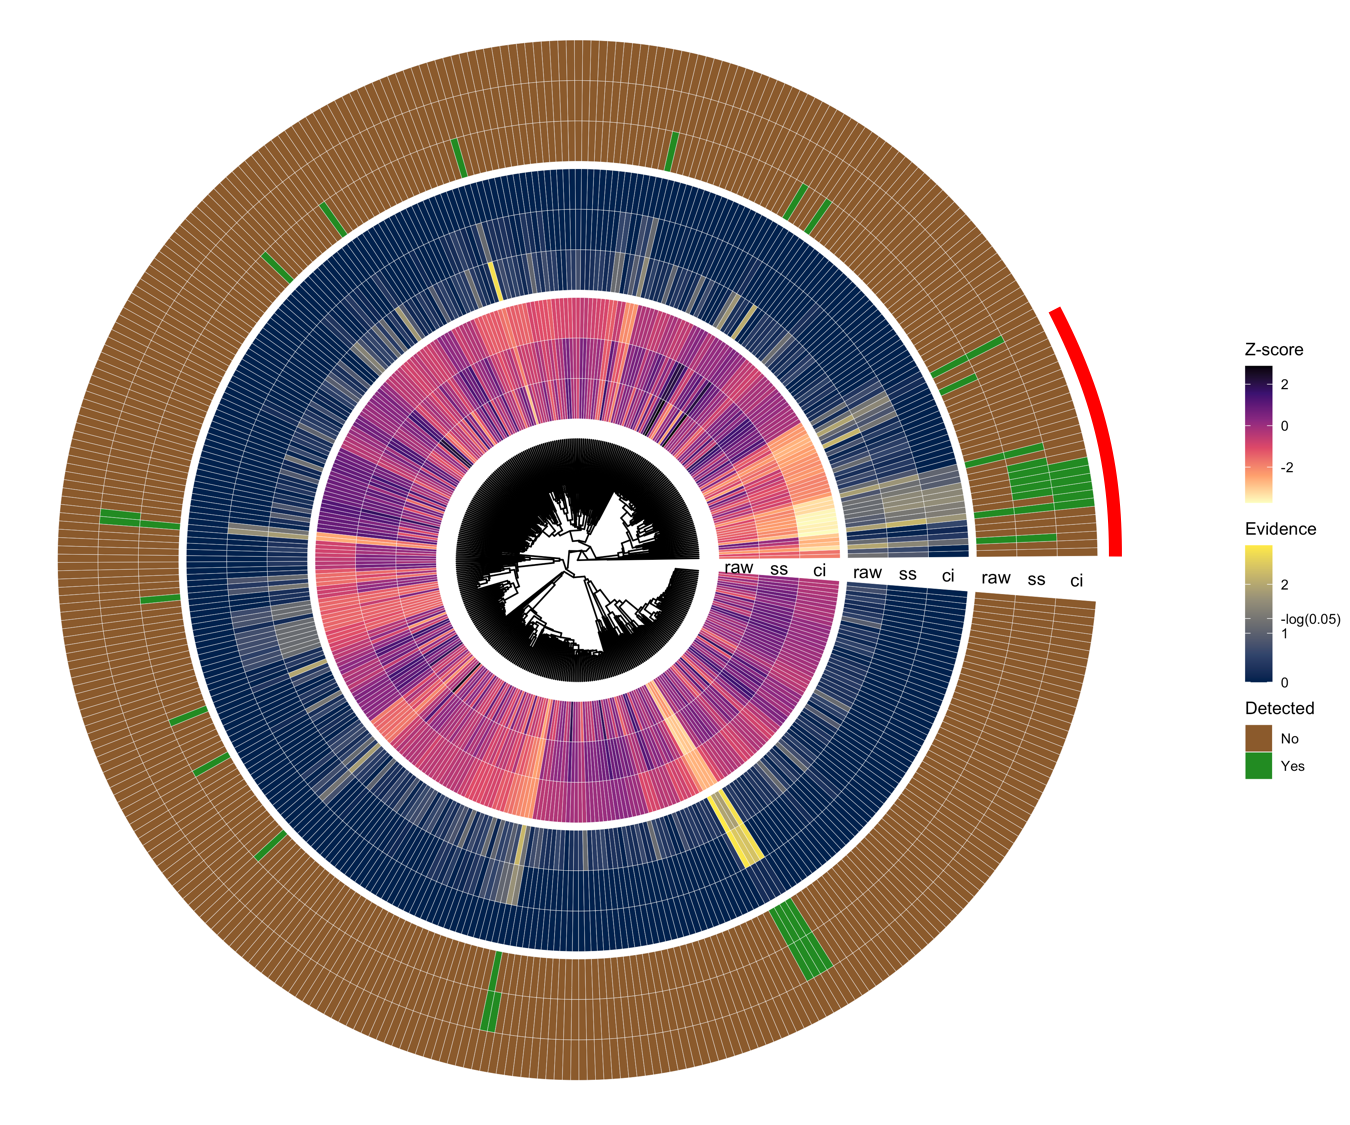
\includegraphics[width=0.9\linewidth]{img/heattree} 

}

\caption{Phylogénie des \(387\) espèces du jeu de données des Fidjiens. Les cercles intérieur, central et extérieur représentent respectivement les \(z\)-scores bruts, les évidences corrigées et les statuts détecté ou non associé aux espèces pour différentes procédures (sans correction et les deux variantes de \emph{zazou}).}\label{fig:heattree}
\end{figure}
\hypertarget{ananum}{%
\chapter{Problèmes d'analyse numérique}\label{ananum}}

Ce chapitre présente trois résolutions que nous avons apportées aux problèmes d'analyses numériques rencontrés lors de l'élaboration de l'algorithme \emph{zazou}, présenté dans la section \ref{zazousection}.

Ce sont des algorithmes itératifs qui permettent de converger jusqu'à une approximation raisonnable de la solution.

\hypertarget{shooting}{%
\section{\texorpdfstring{Algorithme du \emph{shooting}}{Algorithme du shooting}}\label{shooting}}

L'algorithme du \emph{shooting} est une méthode de résolution numérique du lasso proposée par Fu (\protect\hyperlink{ref-fu1998penalized}{1998}). Nous allons ici décrire la variante que nous avons développée lorsque l'espace d'existence du paramètre est contraint.

Le problème \eqref{eq:lasso} peut-être réécrit dans sa forme générale
\begin{equation}
\label{eq:shooting}
\param^\star = \argmin_{\param \in \RR^p,U\param \in \RR^q_{-}} \left\|y - X\param\right\|_2^2 + \lambda \|\param\|_1,
\end{equation}
où \(y \in \RR^n\), \(X \in \RR^{n\times p}\) et \(U \in \RR^{q \times p}\). Il s'agit d'un problème convexe et donc nous pouvons facilement adapter l'algorithme initial pour résoudre itérativement un problème unidirectionnel sur chaque coordonnée.

Pour isoler la \(j^{\text{ème}}\) coordonnée \(\param_j\), nous décomposons les termes du problème en\\
\begin{equation*}
\left\|y - X\param\right\|_2^2 + \lambda \|\param\|_1 = \left\|y - X_{-j}\param_{-j} - \param_j x_j\right\|_2^2 + \lambda |\param_j| + \lambda \|\param_{-j}\|_1
\end{equation*}
et
\begin{equation*}
U\param = U_{-j}\param_{-j} + \param_j u_j.
\end{equation*}
Ainsi, le problème unidirectionnel associé à la \(j^{\text{ème}}\) coordonnée du problème \eqref{eq:shooting} est
\begin{equation}
\label{eq:unidirectionnel}
\left\{
  \begin{aligned}
    \argmin_{\param \in \RR} h(\param) & = \frac{1}{2} \|y - z - x\param\|^2_2 + \lambda |\param| \\
    & \text{t.q. } u + v\param \leq 0
  \end{aligned}
\right.
\end{equation}
Notons \(I_+ = \left\{ i : v_i > 0 \right\}\) et \(I_- = \left\{i : v_i < 0 \right\}\) puis \(\param_{\min} = \max_{i \in I_+} -\frac{u_i}{v_i}\) et \(\param_{\max} = \min_{i \in I_-} -\frac{u_i}{v_i}\).

Le problème \eqref{eq:unidirectionnel} est faisable si et seulement si
\begin{enumerate}
\def\labelenumi{\arabic{enumi}.}
\item
  \(\param_{\min} \leq \param_{\max}\),
\item
  pour chaque \(i\), \(v_i = 0\) entraîne \(u_i \leq 0\).
\end{enumerate}
Sous ces deux conditions, la région de faisabilité est \(\mathcal{I} = \mathopen[\param_{\min}, \param_{\max}\mathclose]\).

Le sous-gradient de \(h\) est
\begin{equation*}
\partial h(\param) = 
\begin{cases} 
-(y-z)^Tx + x^Tx\param - \lambda & \text{si } \param < 0, \\ 
-(y-z)^Tx + x^Tx\param + \lambda & \text{si } \param > 0, \\
 -(y-z)^Tx + \lambda [-1, 1]          & \text{si } \param = 0,
\end{cases}
\end{equation*}
et les potentiels minimiseurs de \(h\), tels que \(0\in \partial h(\param)\), sont alors
\begin{equation}
\label{eq:solutionsanscontrainte}
\begin{cases} 
\frac{(y-z)^Tx+\lambda}{x^Tx} & \text{si } (y-z)^Tx < -\lambda, \\ 
\frac{(y-z)^Tx-\lambda}{x^Tx} & \text{si } (y-z)^Tx > \lambda, \\ 
0                             & \text{si } | (y-z)^Tx | \leq \lambda.
\end{cases}
\end{equation}
Si le problème \eqref{eq:unidirectionnel} est faisable, par convexité de \(h\), sa solution est obtenue en projetant \eqref{eq:solutionsanscontrainte} sur l'ensemble de faisabilité \(\mathcal{I}\) :
\begin{equation*}
\param^\star = \begin{cases} 
P_{\mathcal{I}}\left(\frac{(y-z)^Tx+\lambda}{x^Tx}\right) & \text{si } (y-z)^Tx < -\lambda, \\ 
P_{\mathcal{I}}\left(\frac{(y-z)^Tx-\lambda}{x^Tx}\right) & \text{si } (y-z)^Tx > \lambda, \\ 
P_{\mathcal{I}}(0)                             & \text{si } | (y-z)^Tx | \leq \lambda,
\end{cases}
\end{equation*}
où \(P_{\mathcal{I}} : x \mapsto \max\left({\param_{\min}}, \min\left(x, \param_{\max}\right)\right)\) est la projection sur \(\mathcal{I}\).

\hypertarget{mam}{%
\section{\texorpdfstring{Minimisation sous contrainte de \(x^TAx\)}{Minimisation sous contrainte de x\^{}TAx}}\label{mam}}

Soit \(A \in \RR^{n\times n}\) une matrice définie positive, \(e\) un vecteur de \(\RR^n\) et \(\gamma\) un réel strictement positif. Nous avons mis en place un algorithme de résolution au problème de minimisation suivant :
\begin{equation}
\label{eq:xax}
\left\{
  \begin{aligned}
    x^\star & = \argmin_{x \in \mathbb{R}^{n}} \ x^TAx \\
    &\text{t.q. }\|Ax - e\|_{\infty} \leq \gamma.
  \end{aligned}
\right.
\end{equation}
D'après le théorème spectral, il existe \(U, D \in \RR^{n\times n}\) et \(\lambda \in \RR_+^n\) tels que
\begin{itemize}
\item
  \(A = UDU^T\),
\item
  \(U^TU = \mathbf{I}_n\),
\item
  \(D = \diag\left(\lambda_1, \ldots, \lambda_n\right)\),
\item
  \(\lambda_1 \geq \dots ... \lambda_r > 0 = \lambda_{r+1} = \dots = \lambda_{n}\) avec \(r = \rang(A)\).
\end{itemize}
La solution \(x^{\star}\) du problème initial \eqref{eq:xax} est liée à la solution \(x^{\diamond}\) du problème complémentaire
\begin{equation}
\label{eq:xaxcomp}
\left\{
  \begin{aligned}
    x^\diamond & = \argmin_{x \in \mathbb{R}^{n}} \ x^TDx \\
    &\text{t.q.}\  \|Bx - e\|_{\infty} \leq \gamma
  \end{aligned}
\right.
\end{equation}
par \(x^\star = Ux^\diamond\), avec \(B = UD\).

La résolution du problème complémentaire \eqref{eq:xaxcomp} se fait en trouvant d'abord un \(x\) dans l'ensemble de faisabilité, par exemple avec la méthode proposée dans la section \ref{proj}, puis en mettant à jour coordonnée par coordonnée jusqu'à convergence.

Pour \(j \in [\![1,n]\!]\), le problème de minimisation de \(x^TDx\) en \(x_j\) peut s'écrire
\begin{equation*}
\argmin_{x_j \in \RR} \lambda x_j^2 + \sum_{k\neq j}x_k^2\lambda_k,
\end{equation*}
dont la solution non contrainte évidente est \(0\), qu'il faudra projeter sur l'ensemble de faisabilité.

Explicitons la contrainte en \(x_j\) donnée dans le problème \eqref{eq:xaxcomp}. Écrivons d'abord la décomposition de \(Bx\) en \(Bx = B_{-j}x_{-j} + x_jb_j = c + x_jb_j\) avec \(c = B_{-j}x_{-j}\in\RR^n\).

On a alors
\begin{equation*}
\begin{aligned}
& \|Bx - e\|_\infty \leq \gamma \\
\iff  & \|c + x_jb_j - e\|_\infty \leq \gamma \\
\iff  & |c_k + x_jb_{k,j} - e_k| \leq \gamma & \forall k \\
\iff  & -\gamma \leq c_k + x_jb_{k,j} - e_k \leq \gamma & \forall k \\
\iff  & -\gamma + e_k - c_k \leq x_jb_{k,j} \leq \gamma + e_k - c_k  & \forall k\\
\iff  & x_j \in \mathopen[l_k, u_k\mathclose] = \mathcal{I}_k & \forall k\\
\iff  & x_j \in \mathopen[\max((l_k)_k) , \min((u_k)_k)\mathclose] = \bigcap_k \mathcal{I}_k = \mathcal{I} \\
\end{aligned}
\end{equation*}
où
\begin{equation*}
l_k = \left\{
  \begin{aligned}
    & \frac{-\gamma + e_k - c_k}{b_{k,j}} & \text{si } b_{k,j} > 0 \\
    & \frac{\gamma + e_k - c_k}{-b_{k,j}} & \text{si } b_{k,j} < 0 \\
    & \left\{  
    \begin{aligned}
      & -\infty & \text{si }|c_k - e_k| \leq \gamma \\
      & +\infty & \text{sinon} \\
    \end{aligned}
    \right. & \text{si } b_{k,j} = 0
  \end{aligned}
\right.
\end{equation*}
et
\begin{equation*}
u_k = \left\{
  \begin{aligned}
      & \frac{\gamma + e_k - c_k}{b_{k,j}} & \text{si } b_{k,j} > 0 \\
      & \frac{-\gamma + e_k - c_k}{-b_{k,j}} & \text{si } b_{k,j} < 0 \\
    & \left\{  
    \begin{aligned}
      & +\infty & \text{si }|c_k - e_k| \leq \gamma \\
      & -\infty & \text{sinon} \\
    \end{aligned}
    \right. & \text{si } b_{k,j} = 0
  \end{aligned}
\right.
\end{equation*}
Le problème \eqref{eq:xaxcomp} est faisable si et seulement si \(\mathcal{I} \neq \emptyset\) si et seulement si \(\max((l_k)_k) \leq \min((u_k)_k)\). Dans ce cas, le minimum sous contrainte est atteint en \(P_\mathcal{I}(0)\), la projection de \(0\) sur \(\mathcal{I}\).
\begin{remark}
\iffalse{} {Remarque. } \fi{}S'il existe un \(k\) tel que \(b_{k,j} = 0\) et \(\left|c_k-e_k\right| > \gamma\) alors \(\mathcal{I} = \mathcal{I}_k = \emptyset\) et le problème n'est pas faisable. À l'inverse, si pour tout \(k\), \(b_{k,j} = 0\) et \(\left|c_k-e_k\right| \leq \gamma\) alors \(\mathcal{I} = \RR\) et la solution est \(0\).
\end{remark}
L'algorithme de résolution avance en mettant à jour la \(j^{\text{ème}}\) coordonnée de \(x^\diamond\) à \(P_\mathcal{I}(0)\) et continue d'itérer sur les coordonnées jusqu'à convergence.

\hypertarget{proj}{%
\section{Projection sur un ensemble de faisabilité}\label{proj}}

Nous appliquons ici le problème de projection sur une intersection d'ensembles convexes au cas rencontré dans le problème \eqref{eq:xaxcomp}, c'est-à-dire quand l'ensemble est de la forme \(\|Mx-e\|_{\infty} < \gamma\).

Formellement, si \(M \in \RR^{m\times n}\), \(e \in \RR^m\) et \(\gamma > 0\), nous cherchons à obtenir un point dans \(\mathcal{C} = \left\{x \in \RR^n, \|Mx-e\|_{\infty} < \gamma \right\}\), que nous supposons non vide.

Définissons \(f:x\mapsto \max\left(f_1(x), \ldots, f_m(x), -\varepsilon\right)\), où \(f_j: x\mapsto \left|m_j^Tx - e_j\right| - \gamma\) et \(\varepsilon > 0\). Comme \(\mathcal{C}\neq\emptyset\), \(\argmin f \subset \mathcal{C}\) et \(\min f = -\varepsilon\).

Nous utilisons une descente du gradient dont les itérations successives sont données par \(x^{(0)} \in \RR^n\) et
\begin{equation*}
x^{(k+1)} = x^{(k)} - \alpha_kg_k
\end{equation*}
où \(\alpha_k\) est le pas et \(g_k = \partial f\left(x^{(k)}\right)\).

Comme \(\min f = -\varepsilon\) est connu, nous pouvons utiliser la longueur de pas de Polyak (Polyak, \protect\hyperlink{ref-polyak1987introduction}{1987})
\begin{equation*}
\alpha_k = \frac{f\left(x^{(k)}\right) + \varepsilon}{\|g_k\|_2^2},
\end{equation*}
qui est optimale en un certain sens.

Il nous reste maintenant à expliciter \(g_k\).

Si pour chaque \(i \in [\![1,m]\!]\), \(f_i\left(x^{(k)}\right) < -\varepsilon\) alors \(x^{(k)} \in \mathcal{C}\) et l'algorithme peut s'arrêter.

Dans le cas contraire, il existe \(j\in [\![1,m]\!]\) tel que \(f\left(x^{(k)}\right) = f_j\left(x^{(k)}\right)\) et alors
\begin{equation*}
\begin{aligned}
g_k & = \partial f_j\left(x^{(k)}\right) \\
& = 
  \begin{cases}
  m_j & \text{si}\ m_j^Tx^{(k)} - e_j > 0,\\
  \mathopen[-m_j, m_j\mathclose] & \text{si}\ m_j^Tx^{(k)} - e_j = 0,\\
  -m_j & \text{si}\ m_j^Tx^{(k)} - e_j < 0,
  \end{cases}
\end{aligned}
\end{equation*}
puis \(\|g_k\|_2^2 = m_j^Tm_j\).

\hypertarget{conclusion-et-perspectives}{%
\chapter*{Conclusion et perspectives}\label{conclusion-et-perspectives}}
\addcontentsline{toc}{chapter}{Conclusion et perspectives}

Dans cette thèse, nous avons exploré différentes pistes d'amélioration des méthodes d'analyse d'abondance différentielle en métagénomique tirant parti d'une information hiérarchique sur les taxons.

Après avoir présenté la métagénomique et les méthodes d'abondance différentielle, hiérarchiques ou non, nous avons introduit dans le chapitre \ref{arbres} l'arbre des corrélations. Par construction, cet arbre regroupe les taxons aux profils d'abondance similaires. Intuitivement, les taxons différemment abondants devraient être regroupés dans l'arbre, c'est-à-dire y former des sous-arbres. Ce regroupement de signal permet aux procédures hiérarchiques utilisant l'arbre des corrélations d'être plus puissantes que celles utilisant la taxonomie ou la phylogénie. Cependant, les méthodes existantes souffrent de gros désavantages : le lissage des \(z\)-scores de Xiao et al. (\protect\hyperlink{ref-xiao2017false}{2017}) a du mal à prendre en compte l'arbre et son avantage comparatif par rapport à BH vient avant tout (i) de sa deuxième étape de calcul des \(p\)-valeurs par permutation et de (ii) son implémentation, qui se rabat sur BH lorsque la procédure hiérarchique ne retrouve pas assez de taxons identifiés par BH. De même, le FDR hiérarchique ne permet pas de contrôler le FDR à un niveau spécifié \emph{ex ante} mais uniquement de calculer un niveau de contrôle \emph{ex post}, à l'issue de la procédure. Dans sa formulation la plus naïve, il est même incapable de descendre de la racine et d'explorer l'arbre lorsqu'on l'applique à certaines types de données, par exemple les données compositionnelles. En conséquence, il est préférable d'utiliser la procédure BH plutôt que ces premières méthodes hiérarchiques.

Devant l'absence de procédures hiérarchiques satisfaisantes, nous avons développé notre propre méthode d'analyse d'abondance différentielle hiérarchique, présentée dans le chapitre \ref{nouvelleapproche} et baptisée \emph{zazou}. Il s'agit d'une combinaison de quatre méthodes statistiques connues que nous avons adaptées à notre problème :
\begin{itemize}
\item
  une modélisation des \(z\)-scores par un processus d'Ornstein-Uhlenbeck sur un arbre avec sauts,
\item
  une régression lasso pour estimer de façon parcimonieuse la localisation des sauts dans l'arbre,
\item
  une procédure de débiaisage du lasso,
\item
  une correction pour tests multiples adaptée au lasso débiaisé.
\end{itemize}
Lorsque les taxons différentiellement abondants respectent la structure de l'arbre, \emph{zazou} est une procédure plus puissante que la procédure BH. Ce n'est en revanche plus le cas lorsque les espèces différentiellement abondantes sont réparties aléatoirement dans l'arbre : la régularisation indue par un arbre non informatif fait alors perdre de la puissance statistique.

Enfin, nous avons proposé des solutions effectives aux problèmes d'analyse numérique rencontrés lors de l'implémentation de cette procédure dans le \emph{package} \texttt{\{zazou\}}.

\hypertarget{association-versus-pruxe9diction}{%
\section*{Association versus prédiction}\label{association-versus-pruxe9diction}}
\addcontentsline{toc}{section}{Association versus prédiction}

Jusqu'à présent, notre intérêt était de trouver les taxons associés à une variable réponse --dits différentiellement abondants-- en répondant à la question : « à partir du statut des échantillons, que peut-on dire des taxons qui les composent ? ». Il est possible de retourner ce problème pour en faire un problème de prédiction : « à partir de la composition des échantillons, que peut-on dire sur leur statut ? ». Ce problème n'a pas été abordé dans ce manuscrit et nous allons tenter de donner ici quelques pistes de réflexion.

L'approche la plus classique pour effectuer des prédictions est la régression linéaire. Dans ce cadre mathématique, Park, Hastie, \& Tibshirani (\protect\hyperlink{ref-park2007averaged}{2007}) ont montré que si des groupes de prédicteurs sont suffisamment corrélés, il est plus intéressant --du point de vue de l'erreur de prédiction-- d'effectuer une régression simple sur la moyenne de leur composantes plutôt que de déterminer un coefficient par variable.

Illustrons ceci par un exemple où il n'y a qu'un seul bloc de variables corrélées et standardisées \(x_{1}, \ldots, x_{m}\) telles que
\begin{equation*}
X^TX = 
\begin{bmatrix}
1 & \rho & \cdots & \rho \\
\rho & 1 & \ddots & \vdots \\
\vdots & \ddots & \ddots &\rho \\
\rho & \cdots & \rho & 1
\end{bmatrix}.
\end{equation*}
Au lieu de modéliser la variable réponse \(y\) par \(y_i\sim \sum_j \beta_j x_{i,j} + \varepsilon_i\), il est préférable d'utiliser \(y_i\sim \beta^\star \sum_j \frac{x_{i,j}}{m} + \varepsilon_i\) dès lors que \(\rho\) est suffisamment proche de \(1\).

Ce résultat est intéressant mais l'analyse est limitée à un design peu réaliste, où la corrélation est identique entre toutes les paires de variables. Des extensions à des designs plus réalistes, avec des groupes disjoints de variables corrélées ou une structure de corrélation connue entre les variables --par exemple de type OU sur un arbre-- seraient intéressantes pour des applications à l'étude du microbiote.

\hypertarget{autres-procuxe9dures-hiuxe9rarchiques}{%
\section*{Autres procédures hiérarchiques}\label{autres-procuxe9dures-hiuxe9rarchiques}}
\addcontentsline{toc}{section}{Autres procédures hiérarchiques}

Si l'on regarde les procédures hiérarchiques existantes, elles prennent toutes en entrée un vecteur de \(p\)-valeurs ou de \(z\)-scores. Pour tester ces méthodes, nous avons eu recours à des tests non paramétriques sur les rangs, comme Wilcoxon ou Kruskal-Wallis. Il serait alors intéressant de regarder la combinaison de tests conçus spécifiquement pour les données métagénomiques, comme ceux présentés dans la section \ref{autres-methodes}, avec des procédures hiérarchiques pour évaluer la plus-value de la hiérarchie pour des procédures de tests sophistiquées.

Dans les méthodes actuelles, la hiérarchie intervient toujours dans un deuxième temps, en tant que structure de lissage ou de correction. À notre connaissance, il n'existe pas de test qui prenne directement en compte cette hiérarchie. Des modèles linéaires à matrice de variance-covariance conditionnée par une hiérarchie pourraient convenir.

Les plus proches sont les modèles gaussiens multivariées utilisées en méthodes comparatives phylogénétiques :
\begin{equation*}
\text{vec}(Z) \sim \mathcal{N}_{np}\left(0, \Sigma \otimes R\right)
\end{equation*}
dans lesquelles \(\Sigma\) capture la dépendances entre taxons (typiquement la matrice de covariance d'un OU sur arbre), \(R\) la dépendance entre observations au sein d'un taxon et où \(\otimes\) est le produit de Kronecker. Ces modèles peuvent être adaptés à des données de comptage en adoptant une approche hiérarchique : \(Z\) est une variable latente et les comptages \(Y\), conditionnellement à \(Z\), sont indépendants et tirées dans une loi discrète, typiquement Poisson ou binomiale négative (avec ou sans excès de zéros). S'ils permettent théoriquement sous cette forme de gérer les données de comptages typiquement observées en métagénomique, ils sont plutôt utilisés en pratique pour faire de la détection de ruptures en écologie (Bastide, Ané, Robin, \& Mariadassou, \protect\hyperlink{ref-bastide2018inference}{2018}) et ne permettent pas à notre connaissance de faire des tests d'abondance différentielle.

\hypertarget{amuxe9lioration-de-zazou}{%
\section*{Amélioration de zazou}\label{amuxe9lioration-de-zazou}}
\addcontentsline{toc}{section}{Amélioration de zazou}

\emph{zazou} souffre d'un léger problème lors de l'inférence des paramètres du processus d'Ornstein-Uhlenbeck sur l'arbre : il arrive parfois que le modèle choisi par le critère BIC ne contienne aucun saut. Si la procédure de débiaisage fait qu'il est ensuite tout de même possible de détecter des taxons différentiellement abondants, on aimerait pouvoir être moins strict dans notre sélection de modèle. D'autres procédures de sélection de modèle via un BIC phylogénétique (Khabbazian, Kriebel, Rohe, \& Ané, \protect\hyperlink{ref-khabbazian2016fast}{2016}) ou une heuristique de pente (Baudry, Maugis, \& Michel, \protect\hyperlink{ref-baudry2012slope}{2012}) ont été testées en alternative au BIC traditionnel mais les résultats ne sont pas convaincants. Dans le contexte de \emph{zazou}, le critère idéal sélectionnerait trop de sauts plutôt que pas assez, l'étape final de tests permettant de filtrer les taxons issus des sauts identifiés à tort.

Une autre piste d'amélioration consiste à adapter l'étape de débiaisage aux hypothèses de notre problème. Lors de l'inférence ponctuelle des sauts, le modèle est en effet conditionné pour que les moyennes aux feuilles soient à valeurs dans \(\RR_-\). Cependant, lors du débiaisage, les valeurs aux feuilles ne sont plus contraintes à vivre dans cette demi-droite. L'imposition de contraintes rend l'analyse plus complexe mais il serait intéressant de vérifier son impact sur les propriétés théorique du débiaisage.

Enfin et dans la lignée du point précédent, bien que l'algorithme se montre efficace, les hypothèses requises pour avoir les résultats théoriques des différentes méthodes employées dans \emph{zazou} ne sont pas complètement respectées. Il serait intéressant de creuser cet aspect théorique.

\hypertarget{digest}{%
\chapter*{Digest}\label{digest}}
\addcontentsline{toc}{chapter}{Digest}

\hypertarget{chapter-i}{%
\section*{Chapter I}\label{chapter-i}}
\addcontentsline{toc}{section}{Chapter I}

Microbiome, defined as the collection of microbes that inhabit a given environment, and metagenome, defined as the collection of their genes, have been the focus of growing attention for over a decade. In the human gut, microbial communities are responsible for carbohydrate degradation (Flint et al., \protect\hyperlink{ref-flint2012microbial}{2012}; Rowland et al., \protect\hyperlink{ref-rowland2018gut}{2018}) and help the immune system to regulate inflammation (Blander et al., \protect\hyperlink{ref-blander2017regulation}{2017}). However, microbiome deregulation can also lead to moderate to severe disease, like Crohn's disease (Morgan et al., \protect\hyperlink{ref-morgan2012dysfunction}{2012}), depression (Foster \& Neufeld, \protect\hyperlink{ref-foster2013gut}{2013}), or necrotizing enterocolitis (Mai et al., \protect\hyperlink{ref-mai2011fecal}{2011}). Food and pharmaceutical industries saw the tremendous potential of the gut microbiome began developing product to take advantage of it. Among a lot of different methods, probiotics to lower depressive symptoms (Pinto-Sanchez et al., \protect\hyperlink{ref-pinto2017probiotic}{2017}), prebiotics to enhance specific bacteria and lower obesity's risk (Sakwinska et al., \protect\hyperlink{ref-sakwinska2017prebiotics}{2017}) or fecal transplant to fight against lethal forms of diarrhea (Van Nood et al., \protect\hyperlink{ref-nood2013duodenal}{2013}) have been tested and proved to be highly efficient.

Several techniques are available to establish the composition of the microbiome. The marker gene sequencing approach, also called metabarcoding, aims at targeting a universal but rapidly evolving gene (usually the 16S rRNA gene when studying bacteria) whose sequence acts as a barcode to identify the species it originates from (Morgan \& Huttenhower, \protect\hyperlink{ref-morgan2012human}{2012}). However, it suffers form several drawbacks like the restriction to bacteria and archaea or the impossibility to obtain any information on the biological functions present in or expressed by the community. To bypass those limitations, the whole genome shotgun (WGS) sequencing approach amplifies all the genetic material to reconstruct a functional and more complete view of of the sample. It comes however with added complexity: the sequences must be mapped to preconstructed reference catalogues (Quince et al., \protect\hyperlink{ref-quince2017shotgun}{2017}).

By construction, metagenomics data consist of counts (number of reads per species or per genes) and can be modeled as such. Several models try to take into account overdispersion by using negative binomial models (Zhang et al., \protect\hyperlink{ref-zhang2017negative}{2017}) or overrepresentation of zeros by using zero-inflated models (Xinyan et al., \protect\hyperlink{ref-xinyan2016zero}{2016}). However, several authors also suggest that the counts are misleading and that metagenomics data are compositional in essence and should be analyzed using an appropriate framework (Gloor \& Reid, \protect\hyperlink{ref-gloor2016compositional}{2016}).

\hypertarget{chapter-ii}{%
\section*{Chapter II}\label{chapter-ii}}
\addcontentsline{toc}{section}{Chapter II}

In order to detect taxa that are differentially abundant between groups, several procedures have been developed. Among them, Wilcoxon-Mann-Whitney (Mann \& Whitney, \protect\hyperlink{ref-mann1947test}{1947}; Wilcoxon, \protect\hyperlink{ref-wilcoxon1992individual}{1992}) and Kruskall-Wallis (Kruskal \& Wallis, \protect\hyperlink{ref-kruskal1952use}{1952}) tests are generic rank-based tests whose null hypothesis is a common count distribution in all groups. There also are specific tests tailored to the count or compositional aspect of sequencing-based omics data like \emph{edgeR} (Robinson et al., \protect\hyperlink{ref-robinson2010edger}{2010}), \emph{DESeq2} (Love et al., \protect\hyperlink{ref-love2014moderated}{2014}), \emph{mbzinb} (Chen et al., \protect\hyperlink{ref-chen2018omnibus}{2018}) or \emph{ALDEx2} (Fernandes et al., \protect\hyperlink{ref-fernandes2014unifying}{2014}). The former two were first designed for transcriptomics data and then imported to microbiome data whereas the latter two were designed from the ground up for microbiome data.

All the previously mentioned tests are univariate: they test one taxon at the time for differential abundance and require a subsequent step of multiple testing correction to avoid a high number of false discoveries. The Benjamini-Hochberg procedure (Benjamini \& Hochberg, \protect\hyperlink{ref-benjamini1995controlling}{1995}) is the best known and most popular of those correction procedures: it control the expected proportion of false discoveries \(\EE{\frac{FP}{TP + FP}}\) at a certain level, defined \emph{a priori}.

Recently, new procedures have been proposed to take a hierarchical structure (mainly phylogeny) into account during differential abundance analyses. \emph{TreeFDR} (Xiao et al., \protect\hyperlink{ref-xiao2017false}{2017}) is a two-steps procedure based on smoothing of \(z\)-scores followed by a permutational correction technique. The smoothing is based on a hierarchical model whose hyperparameters control the level of smoothing. Hierarchical FDR, theorized by Yekutieli (\protect\hyperlink{ref-yekutieli2008hierarchical}{2008}) and implemented by Sankaran \& Holmes (\protect\hyperlink{ref-sankaran2014structssi}{2014}), considers instead a top-down approach: it progresses down the tree, from the root to the leaves, and tests increasingly smaller groups of taxons until it can not reject the null hypothesis anymore. Finally, Huang et al. (\protect\hyperlink{ref-huang2020treeclimbr}{2020}) developed \emph{treeclimbR}, which select differentially abundant clades based on a composite score computed for each internal node of the tree.

\hypertarget{chapter-iii}{%
\section*{Chapter III}\label{chapter-iii}}
\addcontentsline{toc}{section}{Chapter III}

This chapter addresses the questions of which tree to consider in hierarchical approaches. Phylogeny reflects the evolution history between taxa and is created from nucleotidic sequences from the dataset. Taxonomy is a highly polytomic tree of nested ranks that is available in reference databases (Geer et al., \protect\hyperlink{ref-geer2010ncbi}{2010}). We introduce the correlation tree, a tree built from the pairwise correlation matrix of abundance data using a hierarchical clustering procedure.

To compare those trees, we consider several distances. Formally, rooted trees are directed acyclic networks: they can be compared using the Robison-Foulds distance (Robinson \& Foulds, \protect\hyperlink{ref-robinson1981comparison}{1981}) which focuses solely on topologies (trees without branches lengths), the cophenetic distance (Sokal \& Rohlf, \protect\hyperlink{ref-sokal1962comparison}{1962}) which focuses on path lengths in the tree, or the Billera-Holmes-Vogtmann distance (Billera et al., \protect\hyperlink{ref-billera2001geometry}{2001}) which embeds trees in a geometric space and consider shortest paths in that space.

We first investigate whether the phylogeny (or the taxonomy) is close to the correlation tree. We perform pairwise BHV distance computation on forest of trees covering the phylogeny, the correlation tree, bootstrapped versions of correlation tree and the random trees followed by a PCoA. It appears that the phylogeny is neither in the confidence region of the correlation tree, nor closer to the correlation tree than a random tree.

We then apply hierarchical procedures with the different trees. The correlation tree performs better than the phylogeny, as it naturally captures similarity of abundance profiles and thus groups taxons in a relevant way. However, the classical BH procedure outperforms the hierarchical procedure, no matter what tree is used.

\hypertarget{chapter-iv}{%
\section*{Chapter IV}\label{chapter-iv}}
\addcontentsline{toc}{section}{Chapter IV}

The Ornstein-Uhlenbeck process with optimal value \(\ou{\optim}\) is defined as the solution of the stochastic differential equation:
\begin{equation*}
\dx{W_t} = - \ou{\alpha} (W_t - \ou{\optim}) \dx{t} + \ou{\sigma}\dx{B_t}.
\end{equation*}
It is a well suited framework to model evolution of continuous phylogenetic traits (Freckleton et al., \protect\hyperlink{ref-freckleton2003bergmann}{2003}), especially because of its \(\ou{\optim}\) centered Gaussian limit law. It has been used as a basic block to build more complex models, by considering OU processes on a tree and by considering piecewise linear functions for \(\ou{\optim}\) (Bastide et al., \protect\hyperlink{ref-bastide2017detection}{2017}).

We proposed a new model, \emph{zazou}, where the \(z\)-scores arise from an OU process on a tree with shifts on its optimal values. Moreover, we assume that under \(\mathcal{H}_1\), \(\zs_i \sim \normal{\mu_i}{1}\) with \(\mu_i < 0\) (McLachlan \& Peel, \protect\hyperlink{ref-mclachlan2004finite}{2004}) : finding the alternative hypotheses is equivalent to finding the non-zero components of \(\mu\). This can be reframed as a constrained version of the well-known lasso (Tibshirani, \protect\hyperlink{ref-tibshirani1996regression}{1996}) to have a point estimator of the \(\mu_i\). We then enhance this estimator using two desparsifications procedures from Zhang \& Zhang (\protect\hyperlink{ref-zhang2014confidence}{2014}) and Javanmard \& Montanari (\protect\hyperlink{ref-javanmard2014confidence}{2014}) to debias the lasso estimate and build confidence intervals and in turn compute \(p\)-values for each of the components of \(\mu\). Those \(p\)-values act as tree-smoothed \(p\)-values. The last part of \emph{zazou} is the application of a multiple testing correction designed for desparsified lasso (Javanmard et al., \protect\hyperlink{ref-javanmard2019false}{2019}) on the computed \(p\)-values.

We evaluate our procedure on both synthetic and real data. When the tree is informative in the simulations, \emph{zazou} outperforms BH and \emph{TreeFDR} in terms of TPR but does not control the FDR at the correct level. Using a threshold independent approach, we show that \emph{zazou} also outperforms competing methods in terms of ROC curves and AUC values. However, when the tree is not informative, forcing an irrelevant constraint leads to a significant loss of AUC.

\hypertarget{chapter-v}{%
\section*{Chapter V}\label{chapter-v}}
\addcontentsline{toc}{section}{Chapter V}

In this last chapter, we resolved three numerical analysis problems. The proposed algorithms are iterative and converge to a reasonable approximation of the solution.

The first one is a variation of the lasso with a linear constraint :
\begin{equation*}
\left\{
  \begin{aligned}
  \param^\star & = \argmin_{\param \in \RR^p} \left\|y - X\param\right\|_2^2 + \lambda \|\param\|_1 \\
        & \text{s.t. } U\param \in \RR^q_{-}
  \end{aligned}
\right.
\end{equation*}
where \(y \in \RR^n\), \(X \in \RR^{n\times p}\) and \(U \in \RR^{q \times p}\).

The second one is a minimization problem of a quadratic form subject to an infinite norm constraint :
\begin{equation*}
\left\{
  \begin{aligned}
    x^\star & = \argmin_{x \in \mathbb{R}^{n}} \ x^TAx, \\
    &\text{s.t. }\|Ax - e\|_{\infty} \leq \gamma,
  \end{aligned}
\right.
\end{equation*}
where \(A \in \RR^{n\times n}\) is a positive semidefinite matrix, \(e\in \RR^n\) and \(\gamma > 0\).

The final one is a feasibility problem, where the goal is to find an element \(x\) that satisfies:
\begin{equation*}
\left\{x \in \RR^m : \|Mx-e\|_{\infty} < \gamma\right\},
\end{equation*}
with \(M \in \RR^{m\times n}\), \(e \in \RR^m\) and \(\gamma > 0\) sufficiently large.

\hypertarget{conclusions-and-outlooks}{%
\section*{Conclusions and outlooks}\label{conclusions-and-outlooks}}
\addcontentsline{toc}{section}{Conclusions and outlooks}

The issue considered in this manuscript is the detection of differentially abundant taxa among several groups. The inverse problem is a prediction problem where one wants to predict the groups from the taxa. Including hierarchical information for prediction has already been done in a weak manner for linear regression by Park et al. (\protect\hyperlink{ref-park2007averaged}{2007}). The hierarchical information was the partition of variables in groups with high covariance among them. They proved that it is more interesting to estimate one coefficient per group than one per variable.

Existing hierarchical procedures take precomputed \(p\)-values or \(z\)-scores as input. Saying that, hierarchical information always come as a second step, for smoothing or correction. To our knowledge, there is no test that use this information.

\emph{zazou} suffers from a minor problem during model selection. Sometimes, the BIC selected model has no shifts. Alternative model selection procedures (Baudry et al., \protect\hyperlink{ref-baudry2012slope}{2012}; Khabbazian et al., \protect\hyperlink{ref-khabbazian2016fast}{2016}) have been tested but without success. The optimal model selection procedure would select a model with too many shifts, the useless one will be removed by the other steps.

Some theoretical work is still requires. During the desparsification step to constraint shifts on branches such that their sum on the leafs are non-positive, and to check if the hypothesis of the several combined methods are respected.

\appendix

\hypertarget{notations}{%
\chapter{Notations}\label{notations}}

Nous répertorions ici l'ensemble des notations classiques suffisamment courantes pour ne pas être explicitées au fil de l'eau.

\(\NN\) : ensemble des entiers naturels (\(0\) inclus)

\(\RR\) : ensemble des réels

\([\![a,b]\!]\) : \(\mathopen[a,b\mathclose] \cap \NN\)

\(E_+\), \(E_-\) ou \(E^*\) : \(E\) restreint à ses éléments positifs, négatifs ou non nuls

\(E^{n\times m}\) : ensemble des matrices à \(n\) lignes et \(m\) colonnes à coefficients dans \(E\)

\(M^T\) : transposée de \(M\)

\(\left|M\right|\) : déterminant de \(M\)

\(m_j\) : \(j^{\text{ème}}\) colonne de \(M\)

\(m_{i,j}\) : élément de \(M\) à l'intersection de la \(i^{\text{ème}}\) ligne et \(j^{\text{ème}}\) colonne

\(M_{-j}\) : matrice obtenue lorsqu'on retire à \(M\) sa \(j^{\text{ème}}\) colonne

\(\mathbf{I}_n\) : matrice identité de dimension \(n\)

\(\mathbf{1}_{n}\) : matrice colonne de taille \(n\) composée uniquement de \(1\)

\(\diag\left(x_1, \ldots, x_n \right)\) : matrice diagonale dont la diagonale est \(x_1, \ldots, x_n\) définie par \(\left(x_i\delta_{i,j}\right)_{i,j \in [\![ 1, n]\!]}\)

\(\|x\|_q\) : norme \(q \in \NN^*\) d'un vecteur définie par \(\left(\sum_{i=1}^n = |x_i|^q \right)^{\frac{1}{q}}\)

\(\|x\|_\infty\) : norme infinie d'un vecteur définie par \(\max\{|x_1|, \ldots, |x_n|\}\)

\(\langle x, y \rangle\) : produit scalaire entre \(x\) et \(y\)

\(x \vee y\) : maximum entre \(x\) et \(y\)

\(f^{(n)}\) : composée \(n\)-ième de \(f\) avec elle-même

\(\nabla^2 f\) : hessienne de \(f\) définie par \(\nabla^2 f:x\mapsto \left(\partial_i\partial_jf(x)\right)_{i,j} \in \RR^{n\times n}\)

\(\binom{n}{k}\) : coefficient binomial défini par \(\frac{n!}{k!(n-k!)}\)

\(\EE{X}\) : espérance de \(X\)

\(\VV{X}\) : variance de \(X\)

\(\CC{X,Y}\) : covariance entre \(X\) et \(Y\)

\(\unif{E}\) : loi uniforme sur \(E\)

\(\normal{\mu}{\sigma^2}\) : loi normale de moyenne \(\mu\) et de variance \(\sigma^2\)

\(\mathcal{N}_{d}\left(\mu,\Sigma\right)\) : loi normale multidimensionnelle de moyenne \(\mu\) et de matrice de variance-covariance \(\Sigma\) en dimension \(d\)

\(\Phi\) : fonction de répartition de la loi normale centrée réduite

\(\mathcal{H}_0\) : hypothèse nulle

\(\mathcal{H}_1\) : hypothèse alternative

\(\mathbb{H}_0\) : indices des hypothèses dans l'ensemble des vraies hypothèses nulles

\(\indic\) : indicatrice de l'événement \(A\) définie par \(\indic_{A} = \begin{cases}1 & \text{si }A\\ 0 & \text{sinon}\end{cases}\)

\(\delta_{i,j}\) : symbole de Kronecker entre \(i\) et \(j\) défini par \(\delta_{i,j} = \indic_{i=j}\)

\((x_{(1)}, \ldots, x_{(n)})\) : réordonnement du vecteur \(x\) défini par \(x_{(1)} = \min_i x_i\) et \(x_{(p)} = \min_{y \in \{x_1, \ldots, x_n\} \setminus \{x_{(1)}, \ldots, x_{(p - 1)}\}} y\) pour \(p \in [\![2,n]\!]\)

\hypertarget{productions-scientifiques}{%
\chapter{Productions scientifiques}\label{productions-scientifiques}}

\hypertarget{quantifying-the-impact-of-tree-choice-in-metagenomics-differential-abundance-studies-with-r}{%
\section*{Quantifying the impact of tree choice in metagenomics differential abundance studies with R}\label{quantifying-the-impact-of-tree-choice-in-metagenomics-differential-abundance-studies-with-r}}
\addcontentsline{toc}{section}{Quantifying the impact of tree choice in metagenomics differential abundance studies with R}

Ce poster a été présenté à \href{https://www.user2019.fr/posters/}{\emph{UseR! 2019}}, et a remporté le premier prix dans la catégorie \emph{Biostatistique}.

\includepdf[pages=1]{productions/Bichat2019poster.pdf}

\hypertarget{incorporating-phylogenetic-information-in-microbiome-differential-abundance-studies-has-no-effect-on-detection-power-and-fdr-control}{%
\section*{Incorporating Phylogenetic Information in Microbiome Differential Abundance Studies Has No Effect on Detection Power and FDR Control}\label{incorporating-phylogenetic-information-in-microbiome-differential-abundance-studies-has-no-effect-on-detection-power-and-fdr-control}}
\addcontentsline{toc}{section}{Incorporating Phylogenetic Information in Microbiome Differential Abundance Studies Has No Effect on Detection Power and FDR Control}

Cet article a été publié dans \href{https://doi.org/10.3389/fmicb.2020.00649}{\emph{Frontiers in Microbiology}}.


\includepdf[pages=1-13]{productions/Bichat2020incorporating.pdf}

\includepdf[pages=1-7]{productions/Bichat2020incorporating_supp.pdf}

\hypertarget{hierarchical-correction-of-p-values-via-a-tree-running-ornstein-uhlenbeck-process}{%
\section*{Hierarchical correction of p-values via a tree running Ornstein-Uhlenbeck process}\label{hierarchical-correction-of-p-values-via-a-tree-running-ornstein-uhlenbeck-process}}
\addcontentsline{toc}{section}{Hierarchical correction of p-values via a tree running Ornstein-Uhlenbeck process}

Cet article a été soumis et est disponible sur \href{http://arxiv.org/abs/2009.13335}{\emph{arXiv}}.

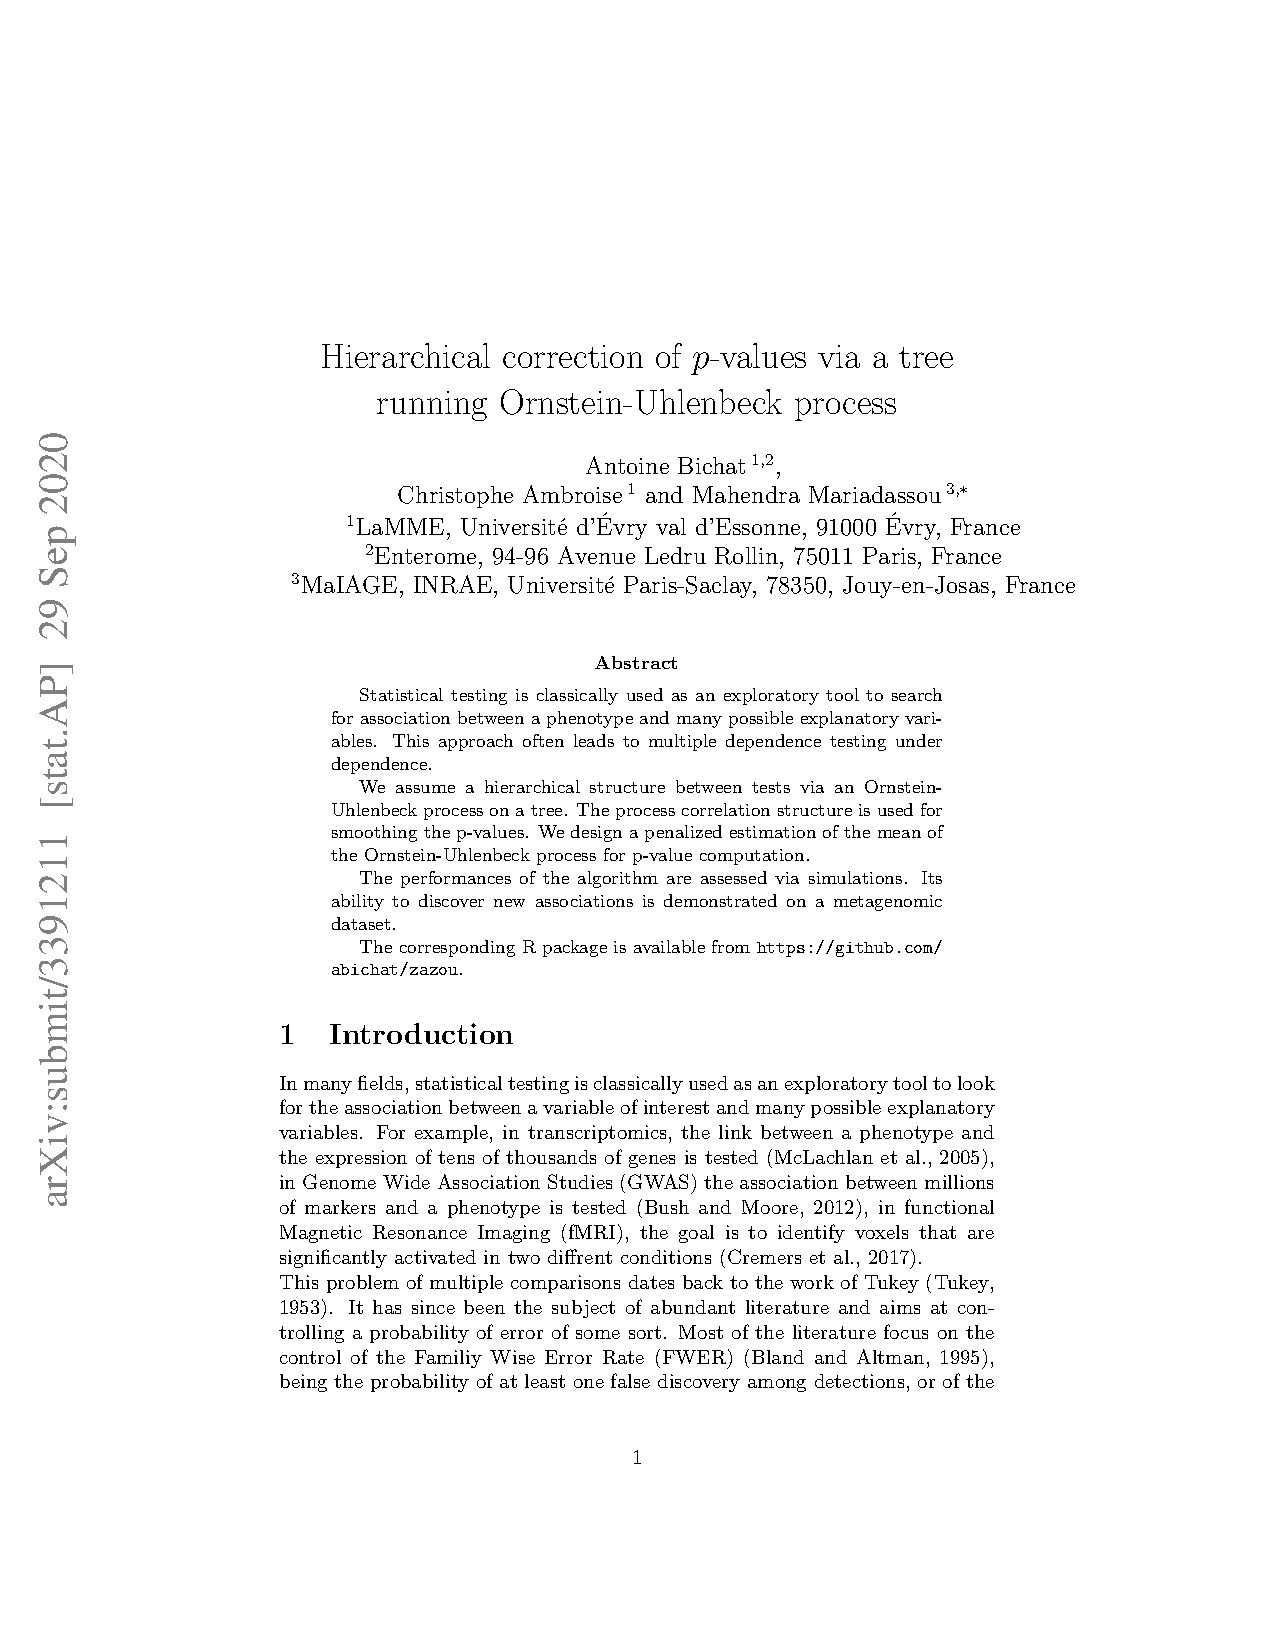
\includepdf[pages=1-13]{productions/Bichat2020hierarchical.pdf}

\hypertarget{packages-r}{%
\section*{Packages R}\label{packages-r}}
\addcontentsline{toc}{section}{Packages R}

\hypertarget{yatah}{%
\subsection*{yatah}\label{yatah}}
\addcontentsline{toc}{subsection}{yatah}

Lorsque l'on travaille avec les données taxonomiques, il est courant d'avoir des lignes taxonomiques écrites sous la forme \texttt{k\_\_Bacteria\textbar{}p\_\_Firmicutes\textbar{}c\_\_Bacilli} pour décrire les différents clades auxquels appartient un taxon donné. \texttt{\{yatah\}} fournit une série de fonctions basées sur des expressions régulières pour manipuler de telles lignées : filtrer les lignées appartenant à un clade spécifique, ne conserver que le dernier rang ou encore créer la table et l'arbre taxonomiques associés. Au moment de la rédaction de ce manuscrit, la version \(0.1.0\) est disponible sur le CRAN.

\hypertarget{evabic}{%
\subsection*{evabic}\label{evabic}}
\addcontentsline{toc}{subsection}{evabic}

\texttt{\{evabic\}}, pour \emph{EVAluation of BInary Classifiers}, permet de calculer facilement des métriques associées à des procédures de classification binaires, typiquement rejet ou non de l'hypothèse nulle. Il a été conçu pour bien s'intégrer dans une logique de code orienté \texttt{\{dplyr\}} et \texttt{\{tidyverse\}} (Wickham et al., \protect\hyperlink{ref-tidyverse2019}{2019}). Au moment de la rédaction de ce manuscrit, la version \(0.0.3\) est disponible sur le CRAN.

\hypertarget{correlationtree}{%
\subsection*{correlationtree}\label{correlationtree}}
\addcontentsline{toc}{subsection}{correlationtree}

La création de l'arbre des corrélations proposée dans la section \ref{cortree} a été implémentée dans le \emph{package} \texttt{\{correlationtree\}}. Au moment de la rédaction de ce manuscrit, la version \(0.0.3\) est disponible sur GitHub.

\hypertarget{zazou}{%
\subsection*{zazou}\label{zazou}}
\addcontentsline{toc}{subsection}{zazou}

L'algorithme \emph{zazou}, décrit dans la section \ref{zazousection}, est implémenté dans le \emph{package} éponyme. Il bénéficie du package \texttt{\{ggtree\}} (Yu, Smith, Zhu, Guan, \& Lam, \protect\hyperlink{ref-yu2017ggtree}{2017}) pour mettre en regard l'arbre et différentes variables associées aux feuilles. Un exemple d'utilisation est donné dans l'annexe \ref{vignette}.

\hypertarget{vignette}{%
\chapter{Vignette de zazou}\label{vignette}}

Nous commençons par charger les \emph{packages} qui seront utilisés dans cette vignette.
\begin{Shaded}
\begin{Highlighting}[]
\KeywordTok{library}\NormalTok{(zazou)}
\KeywordTok{library}\NormalTok{(evabic)}
\KeywordTok{library}\NormalTok{(dplyr)}
\KeywordTok{library}\NormalTok{(ggplot2)}
\KeywordTok{set.seed}\NormalTok{(}\DecValTok{20201209}\NormalTok{)}
\end{Highlighting}
\end{Shaded}
On récupère ensuite le jeu de données de Wu et al. (\protect\hyperlink{ref-wu2011linking}{2011}), où l'on ne conserve que les individus avec une faible consommation d'alcool. On modifie les longueurs de branches de la phylogénie pour que celle-ci soit ultramétrique.
\begin{Shaded}
\begin{Highlighting}[]
\KeywordTok{data}\NormalTok{(}\StringTok{"alcohol"}\NormalTok{)}
\NormalTok{abund <-}\StringTok{ }\NormalTok{alcohol}\OperatorTok{$}\NormalTok{X[, alcohol}\OperatorTok{$}\NormalTok{Y }\OperatorTok{==}\StringTok{ "Low"}\NormalTok{]}
\NormalTok{tree <-}\StringTok{ }\KeywordTok{force_ultrametric}\NormalTok{(alcohol}\OperatorTok{$}\NormalTok{tree)}
\end{Highlighting}
\end{Shaded}
On filtre ensuite les OTUs qui sont présentes dans au moins 25 échantillons parmi les 49.
\begin{Shaded}
\begin{Highlighting}[]
\NormalTok{abund <-}\StringTok{ }\NormalTok{abund[}\KeywordTok{rowSums}\NormalTok{(abund }\OperatorTok{>}\StringTok{ }\DecValTok{0}\NormalTok{) }\OperatorTok{>}\StringTok{ }\DecValTok{25}\NormalTok{, ]}
\NormalTok{tree <-}\StringTok{ }\NormalTok{ape}\OperatorTok{::}\KeywordTok{drop.tip}\NormalTok{(tree, }\KeywordTok{setdiff}\NormalTok{(tree}\OperatorTok{$}\NormalTok{tip.label, }\KeywordTok{rownames}\NormalTok{(abund)))}
\end{Highlighting}
\end{Shaded}
Il en reste alors 91.

Nous assignons ensuite chaque échantillon aléatoirement à un groupe \(A\) ou \(B\).
\begin{Shaded}
\begin{Highlighting}[]
\NormalTok{groups <-}\StringTok{ }\KeywordTok{sample}\NormalTok{(}\KeywordTok{c}\NormalTok{(}\StringTok{"A"}\NormalTok{, }\StringTok{"B"}\NormalTok{), }\DataTypeTok{size =} \KeywordTok{ncol}\NormalTok{(abund), }\DataTypeTok{replace =} \OtherTok{TRUE}\NormalTok{)}
\NormalTok{pvalues_original <-}\StringTok{ }\KeywordTok{test_wilcoxon}\NormalTok{(abund, groups)}\OperatorTok{$}\NormalTok{p.value}
\NormalTok{zscores_original <-}\StringTok{ }\KeywordTok{p2z}\NormalTok{(pvalues_original)}
\KeywordTok{sum}\NormalTok{(pvalues_original }\OperatorTok{<}\StringTok{ }\FloatTok{0.05}\NormalTok{)}
\end{Highlighting}
\end{Shaded}
\begin{verbatim}
[1] 7
\end{verbatim}
Certaines OTUs sont déjà considérées comme différentiellement abondantes.

L'ensemble des OTUs est partitionné en \(20\) groupes cohérents avec la phylogénie, comme expliqué dans la section \ref{simuzazou}. Puis \(5\) de ces groupes et les OTUs qu'ils contiennent sont tirés aléatoirement pour être différentiellement abondants.
\begin{Shaded}
\begin{Highlighting}[]
\NormalTok{clustering <-}\StringTok{ }\KeywordTok{create_clusters}\NormalTok{(tree, }\DataTypeTok{N_clusters =} \DecValTok{20}\NormalTok{, }
                              \DataTypeTok{method =} \StringTok{"paraphyletic"}\NormalTok{)}
\NormalTok{clusters_da <-}\StringTok{ }\KeywordTok{sample}\NormalTok{(}\DecValTok{20}\NormalTok{, }\DecValTok{5}\NormalTok{)}
\NormalTok{clusters_da}
\end{Highlighting}
\end{Shaded}
\begin{verbatim}
[1]  5  4  6  1 17
\end{verbatim}
\begin{Shaded}
\begin{Highlighting}[]
\NormalTok{otus_da <-}\StringTok{ }\KeywordTok{names}\NormalTok{(clustering[}\KeywordTok{which}\NormalTok{(clustering }\OperatorTok\StringTok{ }\NormalTok{clusters_da)])}
\DecValTok{1} \OperatorTok{-}\StringTok{ }\KeywordTok{length}\NormalTok{(otus_da) }\OperatorTok{/}\StringTok{ }\KeywordTok{nrow}\NormalTok{(abund)}
\end{Highlighting}
\end{Shaded}
\begin{verbatim}
[1] 0.6483516
\end{verbatim}
On applique ensuite un \emph{fold-change} de \(10\) aux OTUs différentiellement abondants dans le groupe \(B\).
\begin{Shaded}
\begin{Highlighting}[]
\NormalTok{abund[otus_da, groups }\OperatorTok{==}\StringTok{ "B"}\NormalTok{] <-}\StringTok{ }\DecValTok{10} \OperatorTok{*}\StringTok{ }\NormalTok{abund[otus_da,  groups }\OperatorTok{==}\StringTok{ "B"}\NormalTok{]}
\end{Highlighting}
\end{Shaded}
On effectue un test de Wilcoxon sur ce nouveau jeu de données.
\begin{Shaded}
\begin{Highlighting}[]
\NormalTok{pvalues <-}\StringTok{ }\KeywordTok{test_wilcoxon}\NormalTok{(abund, groups)}\OperatorTok{$}\NormalTok{p.value}
\NormalTok{zscores <-}\StringTok{ }\KeywordTok{p2z}\NormalTok{(pvalues)}
\KeywordTok{plot_shifts}\NormalTok{(tree, }\OtherTok{NA}\NormalTok{, }\DataTypeTok{obs_scores =}\NormalTok{ zscores,}
            \DataTypeTok{sup_scores =} \KeywordTok{list}\NormalTok{(}
              \KeywordTok{list}\NormalTok{(}\DataTypeTok{scores =}\NormalTok{ clustering,}
                   \DataTypeTok{title =} \StringTok{"Clusters"}\NormalTok{,}
                   \DataTypeTok{color =} \KeywordTok{as.character}\NormalTok{(clustering)),}
              \KeywordTok{list}\NormalTok{(}\DataTypeTok{scores =}\NormalTok{ zscores }\OperatorTok{-}\StringTok{ }\NormalTok{zscores_original,}
                   \DataTypeTok{title =} \StringTok{"Difference in z-scores after fold-change"}\NormalTok{,}
                   \DataTypeTok{color =} \KeywordTok{as.character}\NormalTok{(}\KeywordTok{sign}\NormalTok{(zscores }\OperatorTok{-}\StringTok{ }\NormalTok{zscores_original)))}
\NormalTok{              ))}
\end{Highlighting}
\end{Shaded}
\begin{center}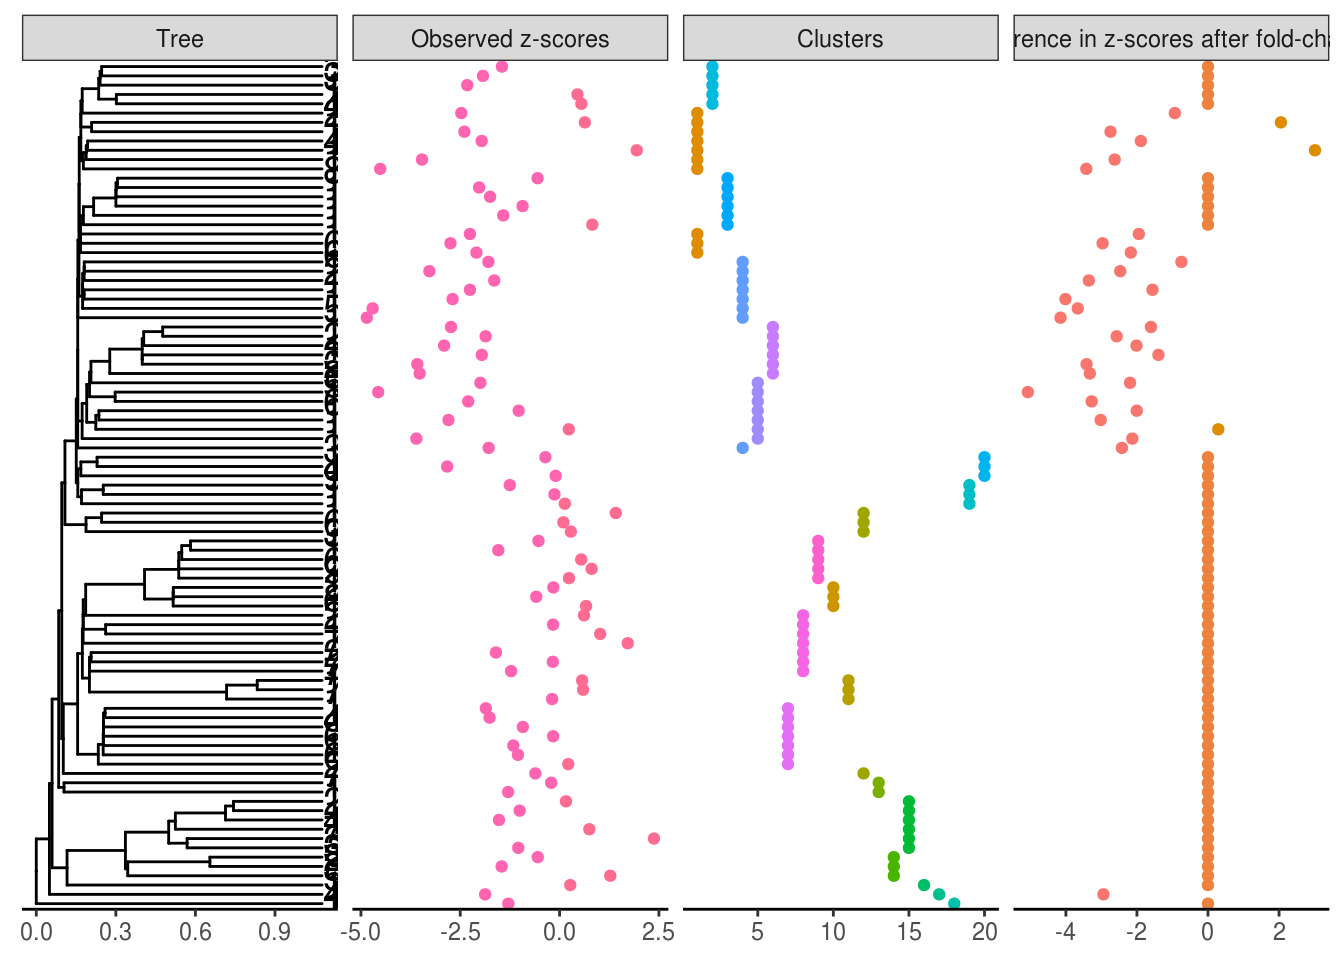
\includegraphics[width=0.9\linewidth]{thesis_files/figure-latex/unnamed-chunk-9-1} \end{center}

Nous donnons ensuite nos \(z\)-scores à la fonction \texttt{estimate\_shifts} pour déterminer la position idéale des sauts avec une régression lasso. La grille des \(\ou{\alpha}\) est également spécifiée mais celle des \(\lambda\) est déterminée automatiquement.
\begin{Shaded}
\begin{Highlighting}[]
\NormalTok{estimation_lasso <-}\StringTok{ }\KeywordTok{estimate_shifts}\NormalTok{(}\DataTypeTok{zscores =}\NormalTok{ zscores, }\DataTypeTok{tree =}\NormalTok{ tree, }
                                    \DataTypeTok{alphaOU =} \KeywordTok{c}\NormalTok{(}\FloatTok{0.2}\NormalTok{, }\FloatTok{0.5}\NormalTok{, }\DecValTok{1}\NormalTok{, }\DecValTok{2}\NormalTok{, }\DecValTok{5}\NormalTok{),}
                                    \DataTypeTok{method =} \StringTok{"lasso"}\NormalTok{)}
\NormalTok{estimation_lasso}
\end{Highlighting}
\end{Shaded}
\begin{verbatim}
Tree is binary with 91 leafs and 180 branches
Covariance matrix has been estimated from an OU with alpha = 5 and sigma = 3.162 
---
Method: lasso with model selection
Regularization parameter: lambda = 14.068 
Objective value: 100.466
BIC: 333.88
pBIC: 372.38
---
Estimated shifts: 0 -0.217 0 0 0 0 -0.539 -0.943 0 0 ...
3 shifts have been identified (ie 98.3 % of sparsity)
A parsimonious solution would involve 3 shifts
---
Observed z-scores:  -2.474 -1.929 -1.451 -2.324 0.549 0.45 -2.397 0.636 -3.463 1.943 ...
Estimated z-scores:   -1.7   -1.7   -1.7   -1.7  -1.7 -1.7   -1.7  -1.7   -1.7  -1.7 ...
90 z-scores have been shifted (ie 1.1 % of sparsity)
\end{verbatim}
\begin{Shaded}
\begin{Highlighting}[]
\KeywordTok{plot}\NormalTok{(estimation_lasso)}
\end{Highlighting}
\end{Shaded}
\begin{center}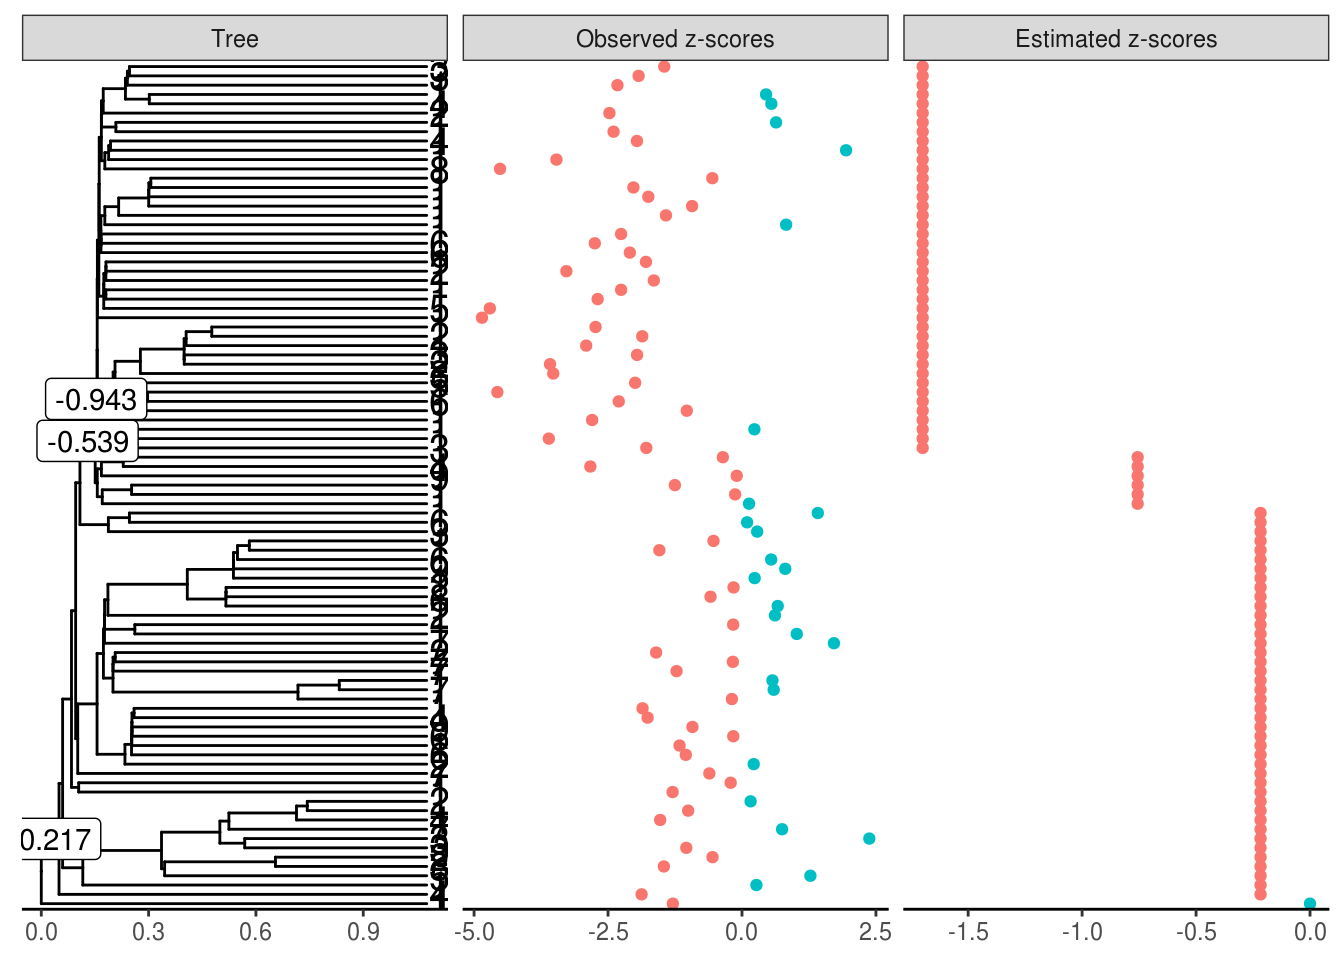
\includegraphics[width=0.9\linewidth]{thesis_files/figure-latex/unnamed-chunk-10-1} \end{center}

Trois sauts sur l'arbre ont été détectés, sur des branches ayant beaucoup de descendants.

Si nous voulons avoir des \(p\)-valeurs et des intervalles de confiance, il faut utiliser une régression \emph{scaled lasso} avant d'appliquer la fonction \texttt{estimate\_confint}.
\begin{Shaded}
\begin{Highlighting}[]
\NormalTok{estimation_scaledlasso <-}\StringTok{ }
\StringTok{  }\KeywordTok{estimate_shifts}\NormalTok{(}\DataTypeTok{zscores =}\NormalTok{ zscores,}
                  \DataTypeTok{tree =}\NormalTok{ tree, }\DataTypeTok{alphaOU =} \KeywordTok{c}\NormalTok{(}\FloatTok{0.2}\NormalTok{, }\FloatTok{0.5}\NormalTok{, }\DecValTok{1}\NormalTok{, }\DecValTok{2}\NormalTok{, }\DecValTok{5}\NormalTok{),}
                  \DataTypeTok{method =} \StringTok{"scaled lasso"}\NormalTok{)}
\NormalTok{estimation_scoresystem <-}\StringTok{ }
\StringTok{  }\KeywordTok{estimate_confint}\NormalTok{(estimation_scaledlasso, }
                   \DataTypeTok{method =} \StringTok{"score system"}\NormalTok{)}
\end{Highlighting}
\end{Shaded}
\begin{verbatim}
t_star is not feasible, falling back to default value.
\end{verbatim}
\begin{Shaded}
\begin{Highlighting}[]
\NormalTok{estimation_scoresystem}
\end{Highlighting}
\end{Shaded}
\begin{verbatim}
Tree is binary with 91 leafs and 180 branches
Method: score system 
Confidence threshold: 0.05 
---
z-scores:
   leaf   estimate     lower      upper     pvalue    qvalue
1   283 -12.887241 -25.64441 -0.1300754 0.02385467 0.8941353
2  3494 -13.363635 -29.06041  2.3331434 0.04759456 1.0000000
3  3470 -12.803510 -28.47336  2.8663408 0.05463910 1.0000000
4  1661 -13.171378 -27.61457  1.2718194 0.03693836 1.0000000
5  4206  -7.310320 -21.70978  7.0891438 0.15985974 1.0000000
6 10038  -7.386608 -21.75859  6.9853783 0.15688556 1.0000000
  ...
\end{verbatim}
\begin{Shaded}
\begin{Highlighting}[]
\KeywordTok{plot}\NormalTok{(estimation_scoresystem)}
\end{Highlighting}
\end{Shaded}
\begin{center}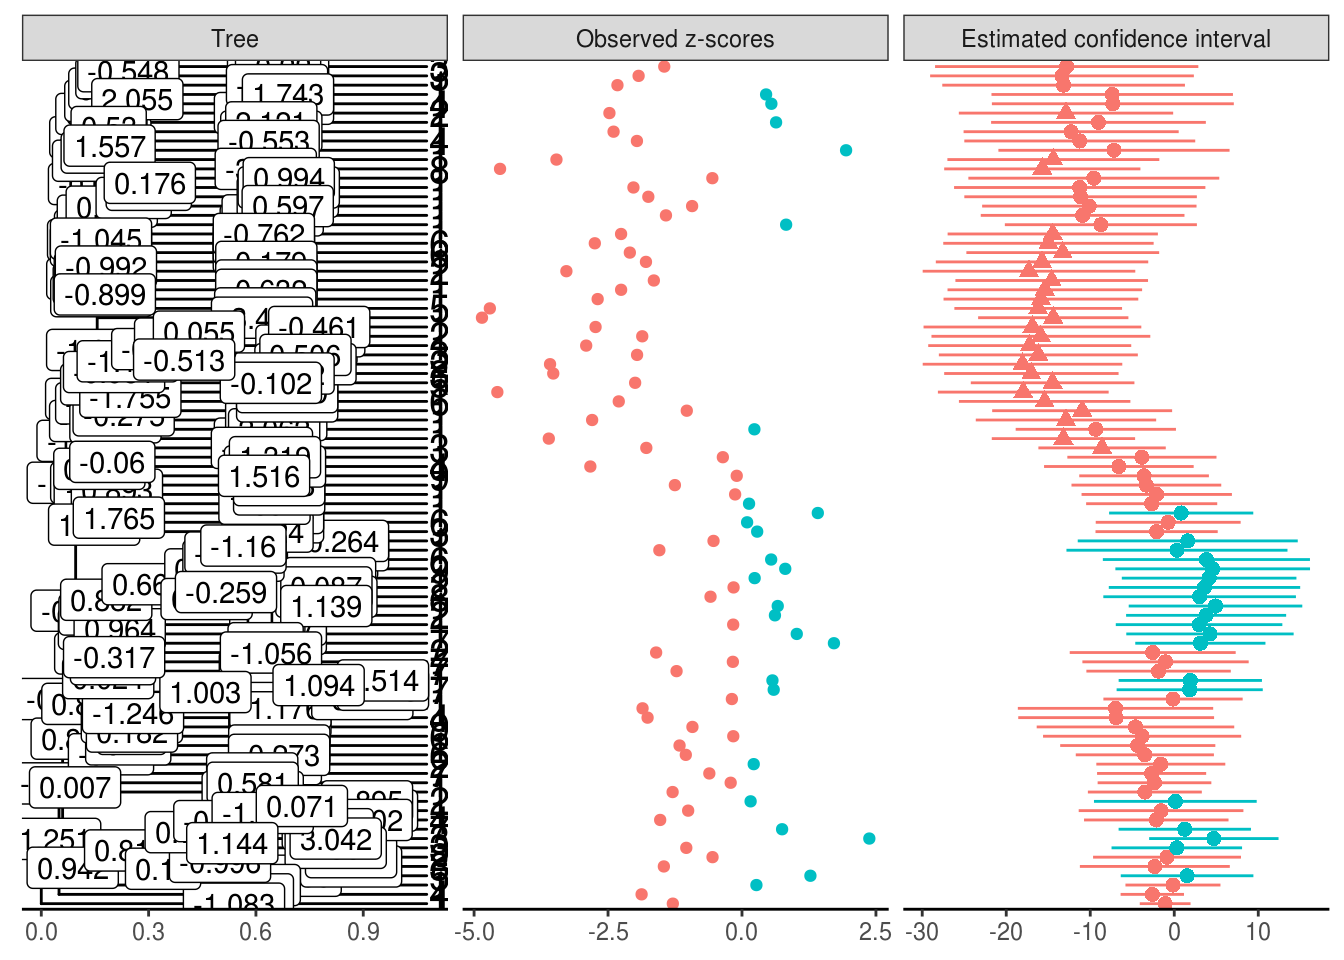
\includegraphics[width=0.9\linewidth]{thesis_files/figure-latex/unnamed-chunk-11-1} \end{center}
\begin{Shaded}
\begin{Highlighting}[]
\NormalTok{pvalues_smoothed <-}\StringTok{ }\KeywordTok{pull_pvalues}\NormalTok{(estimation_scoresystem)}
\end{Highlighting}
\end{Shaded}
Après le débiaisage, les sauts dans les branches ne sont plus parcimonieux.

Nous allons regarder les performances de notre prédicteur via une courbe ROC.
\begin{Shaded}
\begin{Highlighting}[]
\NormalTok{df_measures_zazou <-}\StringTok{ }
\StringTok{  }\KeywordTok{ebc_tidy_by_threshold}\NormalTok{(}\DataTypeTok{detection_values =}\NormalTok{ pvalues_smoothed, }
                        \DataTypeTok{true =}\NormalTok{ otus_da, }\DataTypeTok{all =} \KeywordTok{rownames}\NormalTok{(abund))}
\NormalTok{df_measures_classic <-}\StringTok{ }
\StringTok{  }\KeywordTok{ebc_tidy_by_threshold}\NormalTok{(}\DataTypeTok{detection_values =}\NormalTok{ pvalues, }
                        \DataTypeTok{true =}\NormalTok{ otus_da, }\DataTypeTok{all =} \KeywordTok{rownames}\NormalTok{(abund))}
\KeywordTok{bind_rows}\NormalTok{(}\KeywordTok{mutate}\NormalTok{(df_measures_zazou, }\DataTypeTok{type =} \StringTok{"zazou"}\NormalTok{),}
          \KeywordTok{mutate}\NormalTok{(df_measures_classic, }\DataTypeTok{type =} \StringTok{"classic"}\NormalTok{)) }\OperatorTok\StringTok{ }
\StringTok{  }\KeywordTok{ggplot}\NormalTok{() }\OperatorTok{+}
\StringTok{  }\KeywordTok{aes}\NormalTok{(}\DataTypeTok{x =}\NormalTok{ FPR, }\DataTypeTok{y =}\NormalTok{ TPR, }\DataTypeTok{color =}\NormalTok{ type) }\OperatorTok{+}
\StringTok{  }\KeywordTok{geom_line}\NormalTok{() }\OperatorTok{+}
\StringTok{  }\KeywordTok{theme_bw}\NormalTok{()}
\end{Highlighting}
\end{Shaded}
\begin{center}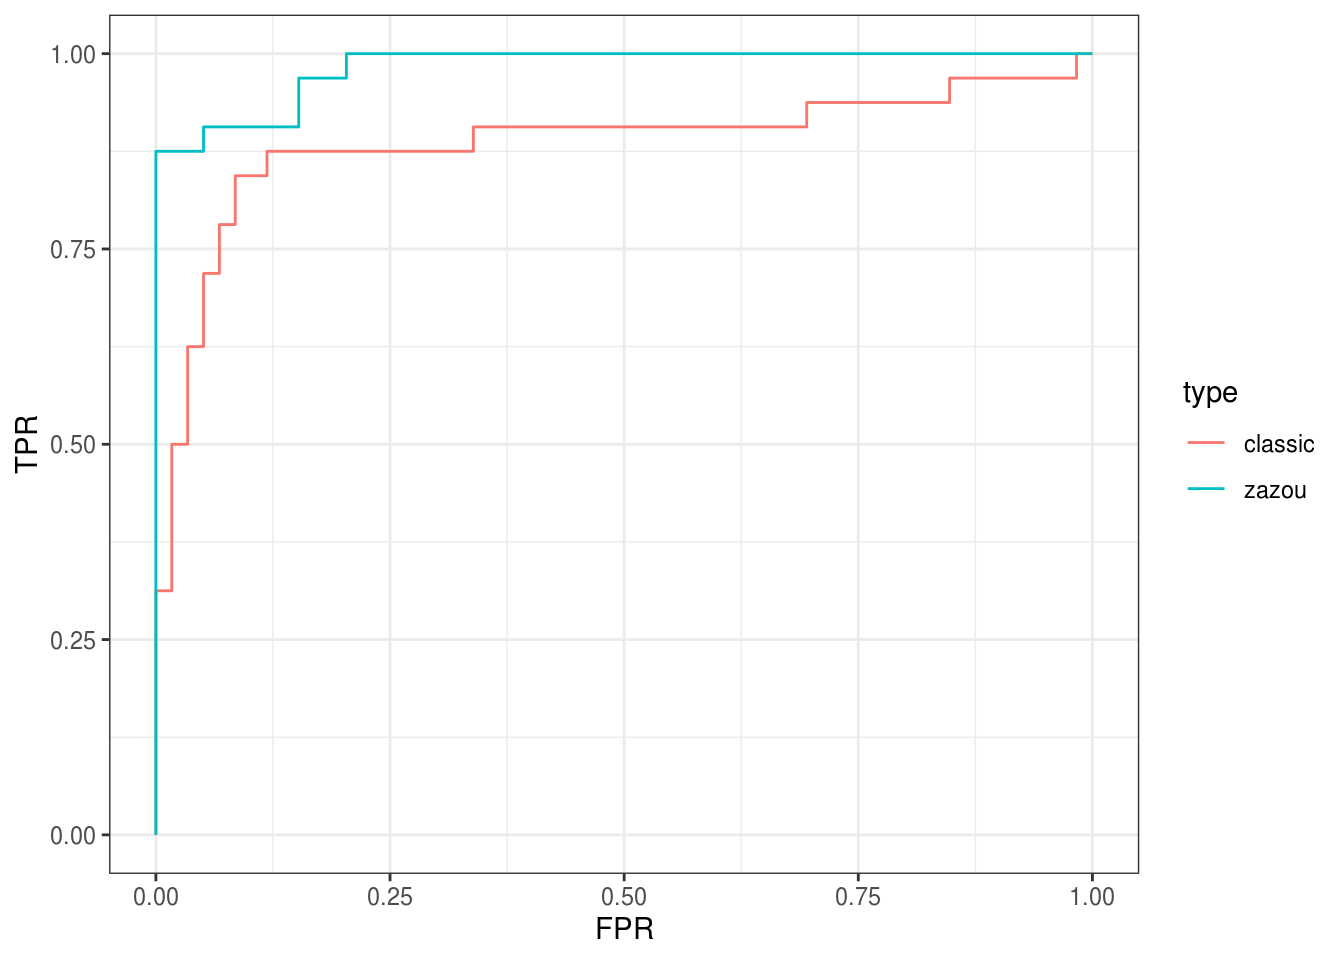
\includegraphics[width=0.9\linewidth]{thesis_files/figure-latex/unnamed-chunk-12-1} \end{center}

La courbe ROC de \emph{zazou} est au dessus de celle de la méthode standard. Et ceci se traduit en terme d'AUC :
\begin{Shaded}
\begin{Highlighting}[]
\KeywordTok{ebc_AUC_from_measures}\NormalTok{(df_measures_zazou)}
\end{Highlighting}
\end{Shaded}
\begin{verbatim}
[1] 0.9825212
\end{verbatim}
\begin{Shaded}
\begin{Highlighting}[]
\KeywordTok{ebc_AUC_from_measures}\NormalTok{(df_measures_classic)}
\end{Highlighting}
\end{Shaded}
\begin{verbatim}
[1] 0.8850636
\end{verbatim}
Version de \texttt{\{zazou\}} utilisée dans cette analyse :
\begin{Shaded}
\begin{Highlighting}[]
\KeywordTok{packageVersion}\NormalTok{(}\StringTok{"zazou"}\NormalTok{)}
\end{Highlighting}
\end{Shaded}
\begin{verbatim}
[1] '0.0.1'
\end{verbatim}
\backmatter

\hypertarget{ruxe9fuxe9rences}{%
\chapter*{Références}\label{ruxe9fuxe9rences}}
\addcontentsline{toc}{chapter}{Références}

\markboth{References}{References}

\noindent

\setlength{\parindent}{-0.20in}
\setlength{\leftskip}{0.20in}
\setlength{\parskip}{8pt}

\hypertarget{refs}{}
\leavevmode\hypertarget{ref-abrahamsson2012low}{}%
Abrahamsson, T. R., Jakobsson, H. E., Andersson, A. F., Björkstén, B., Engstrand, L., \& Jenmalm, M. C. (2012). Low diversity of the gut microbiota in infants with atopic eczema. \emph{Journal of Allergy and Clinical Immunology}, \emph{129}(2), 434--440.

\leavevmode\hypertarget{ref-aitchison1982statistical}{}%
Aitchison, J. (1982). The statistical analysis of compositional data. \emph{Journal of the Royal Statistical Society: Series B (Methodological)}, \emph{44}(2), 139--160.

\leavevmode\hypertarget{ref-aitchison1986statistical}{}%
Aitchison, J. (1986). The statistical analysis of compositional data. Monographs on statistics and applied probability (reprinted in 2003).

\leavevmode\hypertarget{ref-albarede1996introduction}{}%
Albarède, F. (1996). \emph{Introduction to geochemical modeling}. Cambridge University Press.

\leavevmode\hypertarget{ref-almeida2020unified}{}%
Almeida, A., Nayfach, S., Boland, M., Strozzi, F., Beracochea, M., Shi, Z. J., \ldots{} others. (2020). A unified catalog of 204,938 reference genomes from the human gut microbiome. \emph{Nature Biotechnology}, 1--10.

\leavevmode\hypertarget{ref-anders2010differential}{}%
Anders, S., \& Huber, W. (2010). Differential expression analysis for sequence count data. \emph{Nature Precedings}, 1--1.

\leavevmode\hypertarget{ref-araya2020microbiome}{}%
Araya, J. P., González, M., Cardinale, M., Schnell, S., \& Stoll, A. (2020). Microbiome dynamics associated with the atacama flowering desert. \emph{Frontiers in Microbiology}, \emph{10}, 3160.

\leavevmode\hypertarget{ref-aronson2017specific}{}%
Aronson, H. S., Zellmer, A. J., \& Goffredi, S. K. (2017). The specific and exclusive microbiome of the deep-sea bone-eating snail, rubyspira osteovora. \emph{FEMS Microbiology Ecology}, \emph{93}(3), fiw250.

\leavevmode\hypertarget{ref-arumugam2011enterotypes}{}%
Arumugam, M., Raes, J., Pelletier, E., Le Paslier, D., Yamada, T., Mende, D. R., \ldots{} others. (2011). Enterotypes of the human gut microbiome. \emph{Nature}, \emph{473}(7346), 174--180.

\leavevmode\hypertarget{ref-bastide2018inference}{}%
Bastide, P., Ané, C., Robin, S., \& Mariadassou, M. (2018). Inference of adaptive shifts for multivariate correlated traits. \emph{Systematic Biology}, \emph{67}(4), 662--680.

\leavevmode\hypertarget{ref-bastide2017detection}{}%
Bastide, P., Mariadassou, M., \& Robin, S. (2017). Detection of adaptive shifts on phylogenies by using shifted stochastic processes on a tree. \emph{Journal of the Royal Statistical Society: Series B (Statistical Methodology)}, \emph{79}(4), 1067--1093.

\leavevmode\hypertarget{ref-baudry2012slope}{}%
Baudry, J.-P., Maugis, C., \& Michel, B. (2012). Slope heuristics: Overview and implementation. \emph{Statistics and Computing}, \emph{22}(2), 455--470.

\leavevmode\hypertarget{ref-bedarf2017functional}{}%
Bedarf, J. R., Hildebrand, F., Coelho, L. P., Sunagawa, S., Bahram, M., Goeser, F., \ldots{} Wüllner, U. (2017). Functional implications of microbial and viral gut metagenome changes in early stage l-dopa-naïve parkinson's disease patients. \emph{Genome Medicine}, \emph{9}(1), 1--13.

\leavevmode\hypertarget{ref-benjamini1995controlling}{}%
Benjamini, Y., \& Hochberg, Y. (1995). Controlling the false discovery rate: A practical and powerful approach to multiple testing. \emph{Journal of the Royal Statistical Society: Series B (Methodological)}, \emph{57}(1), 289--300.

\leavevmode\hypertarget{ref-benjamini2001control}{}%
Benjamini, Y., \& Yekutieli, D. (2001). The control of the false discovery rate in multiple testing under dependency. \emph{Annals of Statistics}, 1165--1188.

\leavevmode\hypertarget{ref-benoit2016multiple}{}%
Benoit, G., Peterlongo, P., Mariadassou, M., Drezen, E., Schbath, S., Lavenier, D., \& Lemaitre, C. (2016). Multiple comparative metagenomics using multiset k-mer counting. \emph{PeerJ Computer Science}, \emph{2}, e94.

\leavevmode\hypertarget{ref-bichat2020incorporating}{}%
Bichat, A., Plassais, J., Ambroise, C., \& Mariadassou, M. (2020). Incorporating phylogenetic information in microbiome differential abundance studies has no effect on detection power and fdr control. \emph{Frontiers in Microbiology}, \emph{11}, 649. \url{http://doi.org/10.3389/fmicb.2020.00649}

\leavevmode\hypertarget{ref-billera2001geometry}{}%
Billera, L. J., Holmes, S. P., \& Vogtmann, K. (2001). Geometry of the space of phylogenetic trees. \emph{Advances in Applied Mathematics}, \emph{27}(4), 733--767.

\leavevmode\hypertarget{ref-blander2017regulation}{}%
Blander, J. M., Longman, R. S., Iliev, I. D., Sonnenberg, G. F., \& Artis, D. (2017). Regulation of inflammation by microbiota interactions with the host. \emph{Nature Immunology}, \emph{18}(8), 851--860.

\leavevmode\hypertarget{ref-bokulich2016antibiotics}{}%
Bokulich, N. A., Chung, J., Battaglia, T., Henderson, N., Jay, M., Li, H., \ldots{} others. (2016). Antibiotics, birth mode, and diet shape microbiome maturation during early life. \emph{Science Translational Medicine}, \emph{8}(343), 343ra82--343ra82.

\leavevmode\hypertarget{ref-brady2009phymm}{}%
Brady, A., \& Salzberg, S. L. (2009). Phymm and phymmbl: Metagenomic phylogenetic classification with interpolated markov models. \emph{Nature Methods}, \emph{6}(9), 673--676.

\leavevmode\hypertarget{ref-brito2016mobile}{}%
Brito, I. L., Yilmaz, S., Huang, K., Xu, L., Jupiter, S. D., Jenkins, A. P., \ldots{} others. (2016). Mobile genes in the human microbiome are structured from global to individual scales. \emph{Nature}, \emph{535}(7612), 435--439.

\leavevmode\hypertarget{ref-callahan2017exact}{}%
Callahan, B. J., McMurdie, P. J., \& Holmes, S. P. (2017). Exact sequence variants should replace operational taxonomic units in marker-gene data analysis. \emph{The ISME Journal}, \emph{11}(12), 2639--2643.

\leavevmode\hypertarget{ref-callahan2016dada2}{}%
Callahan, B. J., McMurdie, P. J., Rosen, M. J., Han, A. W., Johnson, A. J. A., \& Holmes, S. P. (2016). DADA2: High-resolution sample inference from illumina amplicon data. \emph{Nature Methods}, \emph{13}(7), 581.

\leavevmode\hypertarget{ref-canani2011potential}{}%
Canani, R. B., Di Costanzo, M., Leone, L., Pedata, M., Meli, R., \& Calignano, A. (2011). Potential beneficial effects of butyrate in intestinal and extraintestinal diseases. \emph{World Journal of Gastroenterology: WJG}, \emph{17}(12), 1519.

\leavevmode\hypertarget{ref-caporaso2010qiime}{}%
Caporaso, J. G., Kuczynski, J., Stombaugh, J., Bittinger, K., Bushman, F. D., Costello, E. K., \ldots{} others. (2010). QIIME allows analysis of high-throughput community sequencing data. \emph{Nature Methods}, \emph{7}(5), 335.

\leavevmode\hypertarget{ref-caporaso2011global}{}%
Caporaso, J. G., Lauber, C. L., Walters, W. A., Berg-Lyons, D., Lozupone, C. A., Turnbaugh, P. J., \ldots{} Knight, R. (2011). Global patterns of 16S rRNA diversity at a depth of millions of sequences per sample. \emph{Proceedings of the National Academy of Sciences}, \emph{108}(Supplement 1), 4516--4522.

\leavevmode\hypertarget{ref-cavalli1967phylogenetic}{}%
Cavalli-Sforza, L. L., \& Edwards, A. W. (1967). Phylogenetic analysis. Models and estimation procedures. \emph{American Journal of Human Genetics}, \emph{19}(3 Pt 1), 233.

\leavevmode\hypertarget{ref-cekanaviciute2017gut}{}%
Cekanaviciute, E., Yoo, B. B., Runia, T. F., Debelius, J. W., Singh, S., Nelson, C. A., \ldots{} others. (2017). Gut bacteria from multiple sclerosis patients modulate human t cells and exacerbate symptoms in mouse models. \emph{Proceedings of the National Academy of Sciences}, \emph{114}(40), 10713--10718.

\leavevmode\hypertarget{ref-chaillou2015origin}{}%
Chaillou, S., Chaulot-Talmon, A., Caekebeke, H., Cardinal, M., Christieans, S., Denis, C., \ldots{} others. (2015). Origin and ecological selection of core and food-specific bacterial communities associated with meat and seafood spoilage. \emph{The ISME Journal}, \emph{9}(5), 1105--1118.

\leavevmode\hypertarget{ref-chen2018omnibus}{}%
Chen, J., King, E., Deek, R., Wei, Z., Yu, Y., Grill, D., \& Ballman, K. (2018). An omnibus test for differential distribution analysis of microbiome sequencing data. \emph{Bioinformatics}, \emph{34}(4), 643--651.

\leavevmode\hypertarget{ref-chene2019microbiome}{}%
Chene, L., Sader, C. D., Magalhaes, J., Strozzi, F., Tibaldi, L., Mendez, C., \ldots{} Bonny, C. (2019). Microbiome derived peptides stimulate strong immune response against tumor associated antigens and trigger in vivo tumor regression after vaccination. AACR.

\leavevmode\hypertarget{ref-chong2019microbiome}{}%
Chong, P. P., Chin, V. K., Looi, C. Y., Wong, W. F., Madhavan, P., \& Yong, V. C. (2019). The microbiome and irritable bowel syndrome--a review on the pathophysiology, current research and future therapy. \emph{Frontiers in Microbiology}, \emph{10}, 1136.

\leavevmode\hypertarget{ref-coelho2019ng}{}%
Coelho, L. P., Alves, R., Monteiro, P., Huerta-Cepas, J., Freitas, A. T., \& Bork, P. (2019). NG-meta-profiler: Fast processing of metagenomes using ngless, a domain-specific language. \emph{Microbiome}, \emph{7}(1), 84.

\leavevmode\hypertarget{ref-cuthbertson2014time}{}%
Cuthbertson, L., Rogers, G. B., Walker, A. W., Oliver, A., Hafiz, T., Hoffman, L. R., \ldots{} Van Der Gast, C. J. (2014). Time between collection and storage significantly influences bacterial sequence composition in sputum samples from cystic fibrosis respiratory infections. \emph{Journal of Clinical Microbiology}, \emph{52}(8), 3011--3016.

\leavevmode\hypertarget{ref-david2014diet}{}%
David, L. A., Maurice, C. F., Carmody, R. N., Gootenberg, D. B., Button, J. E., Wolfe, B. E., \ldots{} others. (2014). Diet rapidly and reproducibly alters the human gut microbiome. \emph{Nature}, \emph{505}(7484), 559--563.

\leavevmode\hypertarget{ref-deorowicz2015kmc}{}%
Deorowicz, S., Kokot, M., Grabowski, S., \& Debudaj-Grabysz, A. (2015). KMC 2: Fast and resource-frugal k-mer counting. \emph{Bioinformatics}, \emph{31}(10), 1569--1576.

\leavevmode\hypertarget{ref-desantis2006greengenes}{}%
DeSantis, T. Z., Hugenholtz, P., Larsen, N., Rojas, M., Brodie, E. L., Keller, K., \ldots{} Andersen, G. L. (2006). Greengenes, a chimera-checked 16S rRNA gene database and workbench compatible with arb. \emph{Applied and Environmental Microbiology}, \emph{72}(7), 5069--5072.

\leavevmode\hypertarget{ref-ding2019selective}{}%
Ding, X., Zhang, F., Li, Q., Ting, Z., Cui, B., \& Li, P. (2019). Selective microbiota transplantation is effective for controlling tourette's syndrome. \emph{Gastroenterology}, \emph{156}(6), S--456.

\leavevmode\hypertarget{ref-edgar2010search}{}%
Edgar, R. C. (2010). Search and clustering orders of magnitude faster than blast. \emph{Bioinformatics}, \emph{26}(19), 2460--2461.

\leavevmode\hypertarget{ref-edgar2016uchime2}{}%
Edgar, R. C. (2016). UCHIME2: Improved chimera prediction for amplicon sequencing. \emph{BioRxiv}, 074252.

\leavevmode\hypertarget{ref-egozcue2003isometric}{}%
Egozcue, J. J., Pawlowsky-Glahn, V., Mateu-Figueras, G., \& Barcelo-Vidal, C. (2003). Isometric logratio transformations for compositional data analysis. \emph{Mathematical Geology}, \emph{35}(3), 279--300.

\leavevmode\hypertarget{ref-ekekezie2020understanding}{}%
Ekekezie, C., Perler, B. K., Wexler, A., Duff, C., Lillis, C. J., \& Kelly, C. R. (2020). Understanding the scope of do-it-yourself fecal microbiota transplant. \emph{American Journal of Gastroenterology}, \emph{115}(4), 603--607.

\leavevmode\hypertarget{ref-eloe2013impact}{}%
Eloe-Fadrosh, E. A., McArthur, M. A., Seekatz, A. M., Drabek, E. F., Rasko, D. A., Sztein, M. B., \& Fraser, C. M. (2013). Impact of oral typhoid vaccination on the human gut microbiota and correlations with s. Typhi-specific immunological responses. \emph{PloS One}, \emph{8}(4), e62026.

\leavevmode\hypertarget{ref-eren2014oligotyping}{}%
Eren, A. M., Borisy, G. G., Huse, S. M., \& Welch, J. L. M. (2014). Oligotyping analysis of the human oral microbiome. \emph{Proceedings of the National Academy of Sciences}, \emph{111}(28), E2875--E2884.

\leavevmode\hypertarget{ref-eren2013oligotyping}{}%
Eren, A. M., Maignien, L., Sul, W. J., Murphy, L. G., Grim, S. L., Morrison, H. G., \& Sogin, M. L. (2013). Oligotyping: Differentiating between closely related microbial taxa using 16S rRNA gene data. \emph{Methods in Ecology and Evolution}, \emph{4}(12), 1111--1119.

\leavevmode\hypertarget{ref-fan2015activation}{}%
Fan, D., Coughlin, L. A., Neubauer, M. M., Kim, J., Kim, M. S., Zhan, X., \ldots{} Koh, A. Y. (2015). Activation of hif-1\(\alpha\) and ll-37 by commensal bacteria inhibits candida albicans colonization. \emph{Nature Medicine}, \emph{21}(7), 808.

\leavevmode\hypertarget{ref-felsenstein1985confidence}{}%
Felsenstein, J. (1985). Confidence limits on phylogenies: An approach using the bootstrap. \emph{Evolution}, \emph{39}(4), 783--791.

\leavevmode\hypertarget{ref-fernandes2014unifying}{}%
Fernandes, A. D., Reid, J. N., Macklaim, J. M., McMurrough, T. A., Edgell, D. R., \& Gloor, G. B. (2014). Unifying the analysis of high-throughput sequencing datasets: Characterizing rna-seq, 16S rRNA gene sequencing and selective growth experiments by compositional data analysis. \emph{Microbiome}, \emph{2}(1), 15.

\leavevmode\hypertarget{ref-flint2012microbial}{}%
Flint, H. J., Scott, K. P., Duncan, S. H., Louis, P., \& Forano, E. (2012). Microbial degradation of complex carbohydrates in the gut. \emph{Gut Microbes}, \emph{3}(4), 289--306.

\leavevmode\hypertarget{ref-foster2013gut}{}%
Foster, J. A., \& Neufeld, K.-A. M. (2013). Gut--brain axis: How the microbiome influences anxiety and depression. \emph{Trends in Neurosciences}, \emph{36}(5), 305--312.

\leavevmode\hypertarget{ref-freckleton2003bergmann}{}%
Freckleton, R. P., Harvey, P. H., \& Pagel, M. (2003). Bergmann's rule and body size in mammals. \emph{The American Naturalist}, \emph{161}(5), 821--825.

\leavevmode\hypertarget{ref-fu1998penalized}{}%
Fu, W. J. (1998). Penalized regressions: The bridge versus the lasso. \emph{Journal of Computational and Graphical Statistics}, \emph{7}(3), 397--416.

\leavevmode\hypertarget{ref-geer2010ncbi}{}%
Geer, L. Y., Marchler-Bauer, A., Geer, R. C., Han, L., He, J., He, S., \ldots{} Bryant, S. H. (2010). The ncbi biosystems database. \emph{Nucleic Acids Research}, \emph{38}(suppl\_1), D492--D496.

\leavevmode\hypertarget{ref-gibson2017expert}{}%
Gibson, G. R., Hutkins, R., Sanders, M. E., Prescott, S. L., Reimer, R. A., Salminen, S. J., \ldots{} others. (2017). Expert consensus document: The international scientific association for probiotics and prebiotics (isapp) consensus statement on the definition and scope of prebiotics. \emph{Nature Reviews Gastroenterology \& Hepatology}, \emph{14}(8), 491.

\leavevmode\hypertarget{ref-gloor2017microbiome}{}%
Gloor, G. B., Macklaim, J. M., Pawlowsky-Glahn, V., \& Egozcue, J. J. (2017). Microbiome datasets are compositional: And this is not optional. \emph{Frontiers in Microbiology}, \emph{8}, 2224.

\leavevmode\hypertarget{ref-gloor2016compositional}{}%
Gloor, G. B., \& Reid, G. (2016). Compositional analysis: A valid approach to analyze microbiome high-throughput sequencing data. \emph{Canadian Journal of Microbiology}, \emph{62}(8), 692--703.

\leavevmode\hypertarget{ref-gloor2016relative}{}%
Gloor, G. B., Wu, J. R., Pawlowsky-Glahn, V., \& Egozcue, J. J. (2016). It's all relative: Analyzing microbiome data as compositions. \emph{Annals of Epidemiology}, \emph{26}(5), 322--329.

\leavevmode\hypertarget{ref-gower1966some}{}%
Gower, J. C. (1966). Some distance properties of latent root and vector methods used in multivariate analysis. \emph{Biometrika}, \emph{53}(3-4), 325--338.

\leavevmode\hypertarget{ref-hehemann2010transfer}{}%
Hehemann, J.-H., Correc, G., Barbeyron, T., Helbert, W., Czjzek, M., \& Michel, G. (2010). Transfer of carbohydrate-active enzymes from marine bacteria to japanese gut microbiota. \emph{Nature}, \emph{464}(7290), 908--912.

\leavevmode\hypertarget{ref-holm1979simple}{}%
Holm, S. (1979). A simple sequentially rejective multiple test procedure. \emph{Scandinavian Journal of Statistics}, 65--70.

\leavevmode\hypertarget{ref-holmes2012dirichlet}{}%
Holmes, I., Harris, K., \& Quince, C. (2012). Dirichlet multinomial mixtures: Generative models for microbial metagenomics. \emph{PloS One}, \emph{7}(2), e30126.

\leavevmode\hypertarget{ref-huang2020treeclimbr}{}%
Huang, R., Soneson, C., Germain, P.-L., Schmidt, T., Mering, C. von, \& Robinson, M. (2020). TreeclimbR pinpoints the data-dependent resolution of hierarchical hypotheses. \url{http://doi.org/10.1101/2020.06.08.140608}

\leavevmode\hypertarget{ref-jaglin2018indole}{}%
Jaglin, M., Rhimi, M., Philippe, C., Pons, N., Bruneau, A., Goustard, B., \ldots{} Rabot, S. (2018). Indole, a signaling molecule produced by the gut microbiota, negatively impacts emotional behaviors in rats. \emph{Frontiers in Neuroscience}, \emph{12}, 216.

\leavevmode\hypertarget{ref-javanmard2019false}{}%
Javanmard, A., Javadi, H., \& others. (2019). False discovery rate control via debiased lasso. \emph{Electronic Journal of Statistics}, \emph{13}(1), 1212--1253.

\leavevmode\hypertarget{ref-javanmard2013confidence}{}%
Javanmard, A., \& Montanari, A. (2013). Confidence intervals and hypothesis testing for high-dimensional statistical models. In \emph{Advances in neural information processing systems} (pp. 1187--1195).

\leavevmode\hypertarget{ref-javanmard2014confidence}{}%
Javanmard, A., \& Montanari, A. (2014). Confidence intervals and hypothesis testing for high-dimensional regression. \emph{The Journal of Machine Learning Research}, \emph{15}(1), 2869--2909.

\leavevmode\hypertarget{ref-jiang2017discrete}{}%
Jiang, L., Amir, A., Morton, J. T., Heller, R., Arias-Castro, E., \& Knight, R. (2017). Discrete false-discovery rate improves identification of differentially abundant microbes. \emph{MSystems}, \emph{2}(6).

\leavevmode\hypertarget{ref-jombart2017treespace}{}%
Jombart, T., Kendall, M., Almagro-Garcia, J., \& Colijn, C. (2017). Treespace: Statistical exploration of landscapes of phylogenetic trees. \emph{Molecular Ecology Resources}, \emph{17}(6), 1385--1392.

\leavevmode\hypertarget{ref-jousset2017less}{}%
Jousset, A., Bienhold, C., Chatzinotas, A., Gallien, L., Gobet, A., Kurm, V., \ldots{} others. (2017). Where less may be more: How the rare biosphere pulls ecosystems strings. \emph{The ISME Journal}, \emph{11}(4), 853--862.

\leavevmode\hypertarget{ref-kates2020household}{}%
Kates, A. E., Jarrett, O., Skarlupka, J. H., Sethi, A., Duster, M., Watson, L., \ldots{} Safdar, N. (2020). Household pet ownership and the microbial diversity of the human gut microbiota. \emph{Frontiers in Cellular and Infection Microbiology}, \emph{10}, 73.

\leavevmode\hypertarget{ref-kelly2016gut}{}%
Kelly, T. N., Bazzano, L. A., Ajami, N. J., He, H., Zhao, J., Petrosino, J. F., \ldots{} He, J. (2016). Gut microbiome associates with lifetime cardiovascular disease risk profile among bogalusa heart study participants. \emph{Circulation Research}, \emph{119}(8), 956--964.

\leavevmode\hypertarget{ref-kembel2012incorporating}{}%
Kembel, S. W., Wu, M., Eisen, J. A., \& Green, J. L. (2012). Incorporating 16S gene copy number information improves estimates of microbial diversity and abundance. \emph{PLoS Comput Biol}, \emph{8}(10), e1002743.

\leavevmode\hypertarget{ref-khabbazian2016fast}{}%
Khabbazian, M., Kriebel, R., Rohe, K., \& Ané, C. (2016). Fast and accurate detection of evolutionary shifts in ornstein--uhlenbeck models. \emph{Methods in Ecology and Evolution}, \emph{7}(7), 811--824.

\leavevmode\hypertarget{ref-kim2016centrifuge}{}%
Kim, D., Song, L., Breitwieser, F. P., \& Salzberg, S. L. (2016). Centrifuge: Rapid and sensitive classification of metagenomic sequences. \emph{Genome Research}, \emph{26}(12), 1721--1729.

\leavevmode\hypertarget{ref-kruskal1952use}{}%
Kruskal, W. H., \& Wallis, W. A. (1952). Use of ranks in one-criterion variance analysis. \emph{Journal of the American Statistical Association}, \emph{47}(260), 583--621.

\leavevmode\hypertarget{ref-kultima2012mocat}{}%
Kultima, J. R., Sunagawa, S., Li, J., Chen, W., Chen, H., Mende, D. R., \ldots{} others. (2012). MOCAT: A metagenomics assembly and gene prediction toolkit. \emph{PloS One}, \emph{7}(10), e47656.

\leavevmode\hypertarget{ref-ley2006ecological}{}%
Ley, R. E., Peterson, D. A., \& Gordon, J. I. (2006). Ecological and evolutionary forces shaping microbial diversity in the human intestine. \emph{Cell}, \emph{124}(4), 837--848.

\leavevmode\hypertarget{ref-liu2011accurate}{}%
Liu, B., Gibbons, T., Ghodsi, M., Treangen, T., \& Pop, M. (2011). Accurate and fast estimation of taxonomic profiles from metagenomic shotgun sequences. \emph{Genome Biology}, \emph{12}(1), 1--27.

\leavevmode\hypertarget{ref-love2014moderated}{}%
Love, M. I., Huber, W., \& Anders, S. (2014). Moderated estimation of fold change and dispersion for rna-seq data with deseq2. \emph{Genome Biology}, \emph{15}(12), 550.

\leavevmode\hypertarget{ref-mai2011fecal}{}%
Mai, V., Young, C. M., Ukhanova, M., Wang, X., Sun, Y., Casella, G., \ldots{} others. (2011). Fecal microbiota in premature infants prior to necrotizing enterocolitis. \emph{PloS One}, \emph{6}(6), e20647.

\leavevmode\hypertarget{ref-maidak2000rdp}{}%
Maidak, B. L., Cole, J. R., Lilburn, T. G., Parker Jr, C. T., Saxman, P. R., Stredwick, J. M., \ldots{} others. (2000). The rdp (ribosomal database project) continues. \emph{Nucleic Acids Research}, \emph{28}(1), 173--174.

\leavevmode\hypertarget{ref-maidak1997rdp}{}%
Maidak, B. L., Olsen, G. J., Larsen, N., Overbeek, R., McCaughey, M. J., \& Woese, C. R. (1997). The rdp (ribosomal database project). \emph{Nucleic Acids Research}, \emph{25}(1), 109--110.

\leavevmode\hypertarget{ref-maillet2014commet}{}%
Maillet, N., Collet, G., Vannier, T., Lavenier, D., \& Peterlongo, P. (2014). COMMET: Comparing and combining multiple metagenomic datasets. In \emph{2014 ieee international conference on bioinformatics and biomedicine (bibm)} (pp. 94--98). IEEE.

\leavevmode\hypertarget{ref-maillet2012compareads}{}%
Maillet, N., Lemaitre, C., Chikhi, R., Lavenier, D., \& Peterlongo, P. (2012). Compareads: Comparing huge metagenomic experiments. In \emph{BMC bioinformatics} (Vol. 13, p. S10). Springer.

\leavevmode\hypertarget{ref-mann1947test}{}%
Mann, H. B., \& Whitney, D. R. (1947). On a test of whether one of two random variables is stochastically larger than the other. \emph{The Annals of Mathematical Statistics}, 50--60.

\leavevmode\hypertarget{ref-mathieu1996dna}{}%
Mathieu-Daudé, F., Welsh, J., Vogt, T., \& McClelland, M. (1996). DNA rehybridization during pcr: The `c o t effect'and its consequences. \emph{Nucleic Acids Research}, \emph{24}(11), 2080--2086.

\leavevmode\hypertarget{ref-mcdonald2018american}{}%
McDonald, D., Hyde, E., Debelius, J. W., Morton, J. T., Gonzalez, A., Ackermann, G., \ldots{} others. (2018). American gut: An open platform for citizen science microbiome research. \emph{Msystems}, \emph{3}(3), e00031--18.

\leavevmode\hypertarget{ref-mclachlan2004finite}{}%
McLachlan, G. J., \& Peel, D. (2004). \emph{Finite mixture models}. John Wiley \& Sons.

\leavevmode\hypertarget{ref-mcmurdie2014waste}{}%
McMurdie, P. J., \& Holmes, S. (2014). Waste not, want not: Why rarefying microbiome data is inadmissible. \emph{PLoS Comput Biol}, \emph{10}(4), e1003531.

\leavevmode\hypertarget{ref-meyerhans1990dna}{}%
Meyerhans, A., Vartanian, J.-P., \& Wain-Hobson, S. (1990). DNA recombination during pcr. \emph{Nucleic Acids Research}, \emph{18}(7), 1687--1691.

\leavevmode\hypertarget{ref-modolo2015urqt}{}%
Modolo, L., \& Lerat, E. (2015). UrQt: An efficient software for the unsupervised quality trimming of ngs data. \emph{BMC Bioinformatics}, \emph{16}(1), 137.

\leavevmode\hypertarget{ref-mohty2018odyssee}{}%
Mohty, M., Malard, F., Vekhoff, A., Lapusan, S., Isnard, F., d'Incan, E., \ldots{} others. (2018). The odyssee study: Prevention of dysbiosis complications with autologous fecal microbiota transfer (fmt) in acute myeloid leukemia (aml) patients undergoing intensive treatment: Results of a prospective multicenter trial. In \emph{60th annual meeting of the american-society-of-hematology (ash)} (Vol. 132, p. 4). AMER SOC HEMATOLOGY.

\leavevmode\hypertarget{ref-morgan2012human}{}%
Morgan, X. C., \& Huttenhower, C. (2012). Human microbiome analysis. \emph{PLoS Comput Biol}, \emph{8}(12), e1002808.

\leavevmode\hypertarget{ref-morgan2012dysfunction}{}%
Morgan, X. C., Tickle, T. L., Sokol, H., Gevers, D., Devaney, K. L., Ward, D. V., \ldots{} others. (2012). Dysfunction of the intestinal microbiome in inflammatory bowel disease and treatment. \emph{Genome Biology}, \emph{13}(9), R79.

\leavevmode\hypertarget{ref-otoole2010gut}{}%
O'Toole, P. W., \& Claesson, M. J. (2010). Gut microbiota: Changes throughout the lifespan from infancy to elderly. \emph{International Dairy Journal}, \emph{20}(4), 281--291.

\leavevmode\hypertarget{ref-ounit2015clark}{}%
Ounit, R., Wanamaker, S., Close, T. J., \& Lonardi, S. (2015). CLARK: Fast and accurate classification of metagenomic and genomic sequences using discriminative k-mers. \emph{BMC Genomics}, \emph{16}(1), 236.

\leavevmode\hypertarget{ref-owen2010fast}{}%
Owen, M., \& Provan, J. S. (2010). A fast algorithm for computing geodesic distances in tree space. \emph{IEEE/ACM Transactions on Computational Biology and Bioinformatics}, \emph{8}(1), 2--13.

\leavevmode\hypertarget{ref-palleja2018recovery}{}%
Palleja, A., Mikkelsen, K. H., Forslund, S. K., Kashani, A., Allin, K. H., Nielsen, T., \ldots{} others. (2018). Recovery of gut microbiota of healthy adults following antibiotic exposure. \emph{Nature Microbiology}, \emph{3}(11), 1255--1265.

\leavevmode\hypertarget{ref-park2007averaged}{}%
Park, M. Y., Hastie, T., \& Tibshirani, R. (2007). Averaged gene expressions for regression. \emph{Biostatistics}, \emph{8}(2), 212--227.

\leavevmode\hypertarget{ref-pasolli2017accessible}{}%
Pasolli, E., Schiffer, L., Manghi, P., Renson, A., Obenchain, V., Truong, D. T., \ldots{} others. (2017). Accessible, curated metagenomic data through experimenthub. \emph{Nature Methods}, \emph{14}(11), 1023.

\leavevmode\hypertarget{ref-paulson2013differential}{}%
Paulson, J. N., Stine, O. C., Bravo, H. C., \& Pop, M. (2013). Differential abundance analysis for microbial marker-gene surveys. \emph{Nature Methods}, \emph{10}(12), 1200--1202.

\leavevmode\hypertarget{ref-pawlowsky2007lecture}{}%
Pawlowsky-Glahn, V., Egozcue, J. J., \& Tolosana Delgado, R. (2007). Lecture notes on compositional data analysis.

\leavevmode\hypertarget{ref-philippot2010ecological}{}%
Philippot, L., Andersson, S. G., Battin, T. J., Prosser, J. I., Schimel, J. P., Whitman, W. B., \& Hallin, S. (2010). The ecological coherence of high bacterial taxonomic ranks. \emph{Nature Reviews Microbiology}, \emph{8}(7), 523--529.

\leavevmode\hypertarget{ref-pinto2017probiotic}{}%
Pinto-Sanchez, M. I., Hall, G. B., Ghajar, K., Nardelli, A., Bolino, C., Lau, J. T., \ldots{} others. (2017). Probiotic bifidobacterium longum ncc3001 reduces depression scores and alters brain activity: A pilot study in patients with irritable bowel syndrome. \emph{Gastroenterology}, \emph{153}(2), 448--459.

\leavevmode\hypertarget{ref-pistollato2016role}{}%
Pistollato, F., Sumalla Cano, S., Elio, I., Masias Vergara, M., Giampieri, F., \& Battino, M. (2016). Role of gut microbiota and nutrients in amyloid formation and pathogenesis of alzheimer disease. \emph{Nutrition Reviews}, \emph{74}(10), 624--634.

\leavevmode\hypertarget{ref-plaza2018mspminer}{}%
Plaza Oñate, F., Le Chatelier, E., Almeida, M., Cervino, A. C., Gauthier, F., Magoulès, F., \ldots{} Wren, J. (2018). MSPminer: Abundance-based reconstitution of microbial pan-genomes from shotgun metagenomic data. \emph{Bioinformatics}.

\leavevmode\hypertarget{ref-polyak1987introduction}{}%
Polyak, B. T. (1987). Introduction to optimization. Optimization software. \emph{Inc., Publications Division, New York}, \emph{1}.

\leavevmode\hypertarget{ref-pons2010meteor}{}%
Pons, N., Batto, J.-M., Kennedy, S., Almeida, M., Boumezbeur, F., Moumen, B., \& others. (2010). METEOR, a platform for quantitative metagenomic profiling of complex ecosystems. \emph{Journées Ouvertes En Biologie, Informatique et Mathématiques Http://Www. Jobim2010. Fr/Sites/Default/Files/Presentations/27Pons. Pdf}.

\leavevmode\hypertarget{ref-price2010fasttree}{}%
Price, M. N., Dehal, P. S., \& Arkin, A. P. (2010). FastTree 2--approximately maximum-likelihood trees for large alignments. \emph{PloS One}, \emph{5}(3), e9490.

\leavevmode\hypertarget{ref-qin2012metagenome}{}%
Qin, J., Li, Y., Cai, Z., Li, S., Zhu, J., Zhang, F., \ldots{} others. (2012). A metagenome-wide association study of gut microbiota in type 2 diabetes. \emph{Nature}, \emph{490}(7418), 55--60.

\leavevmode\hypertarget{ref-qin2014alterations}{}%
Qin, N., Yang, F., Li, A., Prifti, E., Chen, Y., Shao, L., \ldots{} others. (2014). Alterations of the human gut microbiome in liver cirrhosis. \emph{Nature}, \emph{513}(7516), 59--64.

\leavevmode\hypertarget{ref-quast2012silva}{}%
Quast, C., Pruesse, E., Yilmaz, P., Gerken, J., Schweer, T., Yarza, P., \ldots{} Glöckner, F. O. (2012). The silva ribosomal rna gene database project: Improved data processing and web-based tools. \emph{Nucleic Acids Research}, \emph{41}(D1), D590--D596.

\leavevmode\hypertarget{ref-quince2017shotgun}{}%
Quince, C., Walker, A. W., Simpson, J. T., Loman, N. J., \& Segata, N. (2017). Shotgun metagenomics, from sampling to analysis. \emph{Nature Biotechnology}, \emph{35}(9), 833--844.

\leavevmode\hypertarget{ref-ravel2011vaginal}{}%
Ravel, J., Gajer, P., Abdo, Z., Schneider, G. M., Koenig, S. S., McCulle, S. L., \ldots{} others. (2011). Vaginal microbiome of reproductive-age women. \emph{Proceedings of the National Academy of Sciences}, \emph{108}(Supplement 1), 4680--4687.

\leavevmode\hypertarget{ref-r2020}{}%
R Core Team. (2020). \emph{R: A language and environment for statistical computing}. Vienna, Austria: R Foundation for Statistical Computing. Retrieved from \url{https://www.R-project.org/}

\leavevmode\hypertarget{ref-reardon2018faecal}{}%
Reardon, S. (2018). Faecal transplants could help preserve vulnerable species. \emph{Nature}, \emph{558}(7709), 173--175.

\leavevmode\hypertarget{ref-regier2019combination}{}%
Regier, Y., Komma, K., Weigel, M., Kraiczy, P., Laisi, A., Pulliainen, A. T., \ldots{} Kempf, V. A. (2019). Combination of microbiome analysis and serodiagnostics to assess the risk of pathogen transmission by ticks to humans and animals in central germany. \emph{Parasites \& Vectors}, \emph{12}(1), 11.

\leavevmode\hypertarget{ref-reynolds2006clustering}{}%
Reynolds, A. P., Richards, G., Iglesia, B. de la, \& Rayward-Smith, V. J. (2006). Clustering rules: A comparison of partitioning and hierarchical clustering algorithms. \emph{Journal of Mathematical Modelling and Algorithms}, \emph{5}(4), 475--504.

\leavevmode\hypertarget{ref-robinson1981comparison}{}%
Robinson, D. F., \& Foulds, L. R. (1981). Comparison of phylogenetic trees. \emph{Mathematical Biosciences}, \emph{53}(1-2), 131--147.

\leavevmode\hypertarget{ref-robinson2010edger}{}%
Robinson, M. D., McCarthy, D. J., \& Smyth, G. K. (2010). EdgeR: A bioconductor package for differential expression analysis of digital gene expression data. \emph{Bioinformatics}, \emph{26}(1), 139--140.

\leavevmode\hypertarget{ref-robinson2007moderated}{}%
Robinson, M. D., \& Smyth, G. K. (2007). Moderated statistical tests for assessing differences in tag abundance. \emph{Bioinformatics}, \emph{23}(21), 2881--2887.

\leavevmode\hypertarget{ref-rowland2018gut}{}%
Rowland, I., Gibson, G., Heinken, A., Scott, K., Swann, J., Thiele, I., \& Tuohy, K. (2018). Gut microbiota functions: Metabolism of nutrients and other food components. \emph{European Journal of Nutrition}, \emph{57}(1), 1--24.

\leavevmode\hypertarget{ref-sakwinska2017prebiotics}{}%
Sakwinska, O., Berger, B., Zolezzi, I. S., \& Holbrook, J. (2017). Prebiotics for reducing the risk of obesity later in life. WO2016026684A1.

\leavevmode\hypertarget{ref-sankaran2014structssi}{}%
Sankaran, K., \& Holmes, S. (2014). StructSSI: Simultaneous and selective inference for grouped or hierarchically structured data. \emph{Journal of Statistical Software}, \emph{59}(13), 1.

\leavevmode\hypertarget{ref-schloss2009introducing}{}%
Schloss, P. D., Westcott, S. L., Ryabin, T., Hall, J. R., Hartmann, M., Hollister, E. B., \ldots{} others. (2009). Introducing mothur: Open-source, platform-independent, community-supported software for describing and comparing microbial communities. \emph{Applied and Environmental Microbiology}, \emph{75}(23), 7537--7541.

\leavevmode\hypertarget{ref-schretter2018gut}{}%
Schretter, C. E., Vielmetter, J., Bartos, I., Marka, Z., Marka, S., Argade, S., \& Mazmanian, S. K. (2018). A gut microbial factor modulates locomotor behaviour in drosophila. \emph{Nature}, \emph{563}(7731), 402--406.

\leavevmode\hypertarget{ref-segata2012metagenomic}{}%
Segata, N., Waldron, L., Ballarini, A., Narasimhan, V., Jousson, O., \& Huttenhower, C. (2012). Metagenomic microbial community profiling using unique clade-specific marker genes. \emph{Nature Methods}, \emph{9}(8), 811--814.

\leavevmode\hypertarget{ref-sergeant2012high}{}%
Sergeant, M. J., Constantinidou, C., Cogan, T., Penn, C. W., \& Pallen, M. J. (2012). High-throughput sequencing of 16S rRNA gene amplicons: Effects of extraction procedure, primer length and annealing temperature. \emph{PloS One}, \emph{7}(5), e38094.

\leavevmode\hypertarget{ref-sharon2010commensal}{}%
Sharon, G., Segal, D., Ringo, J. M., Hefetz, A., Zilber-Rosenberg, I., \& Rosenberg, E. (2010). Commensal bacteria play a role in mating preference of drosophila melanogaster. \emph{Proceedings of the National Academy of Sciences}, \emph{107}(46), 20051--20056.

\leavevmode\hypertarget{ref-silverman2017phylogenetic}{}%
Silverman, J. D., Washburne, A. D., Mukherjee, S., \& David, L. A. (2017). A phylogenetic transform enhances analysis of compositional microbiota data. \emph{Elife}, \emph{6}, e21887.

\leavevmode\hypertarget{ref-sneath1973numerical}{}%
Sneath, P. H., Sokal, R. R., \& others. (1973). \emph{Numerical taxonomy. The principles and practice of numerical classification.}

\leavevmode\hypertarget{ref-sokal1962comparison}{}%
Sokal, R. R., \& Rohlf, F. J. (1962). The comparison of dendrograms by objective methods. \emph{Taxon}, \emph{11}(2), 33--40.

\leavevmode\hypertarget{ref-stoddard2015rrn}{}%
Stoddard, S. F., Smith, B. J., Hein, R., Roller, B. R., \& Schmidt, T. M. (2015). Rrn db: Improved tools for interpreting rRNA gene abundance in bacteria and archaea and a new foundation for future development. \emph{Nucleic Acids Research}, \emph{43}(D1), D593--D598.

\leavevmode\hypertarget{ref-stokholm2018maturation}{}%
Stokholm, J., Blaser, M. J., Thorsen, J., Rasmussen, M. A., Waage, J., Vinding, R. K., \ldots{} others. (2018). Maturation of the gut microbiome and risk of asthma in childhood. \emph{Nature Communications}, \emph{9}(1), 1--10.

\leavevmode\hypertarget{ref-sun2012scaled}{}%
Sun, T., \& Zhang, C.-H. (2012). Scaled sparse linear regression. \emph{Biometrika}, \emph{99}(4), 879--898.

\leavevmode\hypertarget{ref-tibshirani1996regression}{}%
Tibshirani, R. (1996). Regression shrinkage and selection via the lasso. \emph{Journal of the Royal Statistical Society: Series B (Methodological)}, \emph{58}(1), 267--288.

\leavevmode\hypertarget{ref-truong2015metaphlan2}{}%
Truong, D. T., Franzosa, E. A., Tickle, T. L., Scholz, M., Weingart, G., Pasolli, E., \ldots{} Segata, N. (2015). MetaPhlAn2 for enhanced metagenomic taxonomic profiling. \emph{Nature Methods}, \emph{12}(10), 902--903.

\leavevmode\hypertarget{ref-turnbaugh2009core}{}%
Turnbaugh, P. J., Hamady, M., Yatsunenko, T., Cantarel, B. L., Duncan, A., Ley, R. E., \ldots{} others. (2009). A core gut microbiome in obese and lean twins. \emph{Nature}, \emph{457}(7228), 480--484.

\leavevmode\hypertarget{ref-valdez2014influence}{}%
Valdez, Y., Brown, E. M., \& Finlay, B. B. (2014). Influence of the microbiota on vaccine effectiveness. \emph{Trends in Immunology}, \emph{35}(11), 526--537.

\leavevmode\hypertarget{ref-vandeputte2017quantitative}{}%
Vandeputte, D., Kathagen, G., D'hoe, K., Vieira-Silva, S., Valles-Colomer, M., Sabino, J., \ldots{} others. (2017). Quantitative microbiome profiling links gut community variation to microbial load. \emph{Nature}, \emph{551}(7681), 507--511.

\leavevmode\hypertarget{ref-nood2013duodenal}{}%
Van Nood, E., Vrieze, A., Nieuwdorp, M., Fuentes, S., Zoetendal, E. G., Vos, W. M. de, \ldots{} others. (2013). Duodenal infusion of donor feces for recurrent clostridium difficile. \emph{New England Journal of Medicine}, \emph{368}(5), 407--415.

\leavevmode\hypertarget{ref-tidyverse2019}{}%
Wickham, H., Averick, M., Bryan, J., Chang, W., McGowan, L. D., François, R., \ldots{} Yutani, H. (2019). Welcome to the tidyverse. \emph{Journal of Open Source Software}, \emph{4}(43), 1686. \url{http://doi.org/10.21105/joss.01686}

\leavevmode\hypertarget{ref-wilcoxon1992individual}{}%
Wilcoxon, F. (1992). Individual comparisons by ranking methods. In \emph{Breakthroughs in statistics} (pp. 196--202). Springer.

\leavevmode\hypertarget{ref-wilgenbusch2017visualizing}{}%
Wilgenbusch, J. C., Huang, W., \& Gallivan, K. A. (2017). Visualizing phylogenetic tree landscapes. \emph{BMC Bioinformatics}, \emph{18}(1), 85.

\leavevmode\hypertarget{ref-wood2014kraken}{}%
Wood, D. E., \& Salzberg, S. L. (2014). Kraken: Ultrafast metagenomic sequence classification using exact alignments. \emph{Genome Biology}, \emph{15}(3), 1--12.

\leavevmode\hypertarget{ref-wright2012decipher}{}%
Wright, E. S., Yilmaz, L. S., \& Noguera, D. R. (2012). DECIPHER, a search-based approach to chimera identification for 16S rRNA sequences. \emph{Applied and Environmental Microbiology}, \emph{78}(3), 717--725.

\leavevmode\hypertarget{ref-wu2011linking}{}%
Wu, G. D., Chen, J., Hoffmann, C., Bittinger, K., Chen, Y.-Y., Keilbaugh, S. A., \ldots{} others. (2011). Linking long-term dietary patterns with gut microbial enterotypes. \emph{Science}, \emph{334}(6052), 105--108.

\leavevmode\hypertarget{ref-xia2018statistical}{}%
Xia, Y., Sun, J., \& Chen, D.-G. (2018). \emph{Statistical analysis of microbiome data with r}. Springer.

\leavevmode\hypertarget{ref-xiao2017false}{}%
Xiao, J., Cao, H., \& Chen, J. (2017). False discovery rate control incorporating phylogenetic tree increases detection power in microbiome-wide multiple testing. \emph{Bioinformatics}, \emph{33}(18), 2873--2881.

\leavevmode\hypertarget{ref-xinyan2016zero}{}%
Xinyan, Z., Himel, M., \& Nengjun, Y. (2016). Zero-inflated negative binomial regression for differential abundance testing in microbiome studies. \emph{Journal of Bioinformatics and Genomics}, (2), 1--1.

\leavevmode\hypertarget{ref-yatsunenko2012human}{}%
Yatsunenko, T., Rey, F. E., Manary, M. J., Trehan, I., Dominguez-Bello, M. G., Contreras, M., \ldots{} others. (2012). Human gut microbiome viewed across age and geography. \emph{Nature}, \emph{486}(7402), 222--227.

\leavevmode\hypertarget{ref-yekutieli2008hierarchical}{}%
Yekutieli, D. (2008). Hierarchical false discovery rate--controlling methodology. \emph{Journal of the American Statistical Association}, \emph{103}(481), 309--316.

\leavevmode\hypertarget{ref-yu2017ggtree}{}%
Yu, G., Smith, D. K., Zhu, H., Guan, Y., \& Lam, T. T.-Y. (2017). Ggtree: An r package for visualization and annotation of phylogenetic trees with their covariates and other associated data. \emph{Methods in Ecology and Evolution}, \emph{8}(1), 28--36.

\leavevmode\hypertarget{ref-zeller2014potential}{}%
Zeller, G., Tap, J., Voigt, A. Y., Sunagawa, S., Kultima, J. R., Costea, P. I., \ldots{} others. (2014). Potential of fecal microbiota for early-stage detection of colorectal cancer. \emph{Molecular Systems Biology}, \emph{10}(11), 766.

\leavevmode\hypertarget{ref-zhang2014confidence}{}%
Zhang, C.-H., \& Zhang, S. S. (2014). Confidence intervals for low dimensional parameters in high dimensional linear models. \emph{Journal of the Royal Statistical Society: Series B (Statistical Methodology)}, \emph{76}(1), 217--242.

\leavevmode\hypertarget{ref-zhang2012should}{}%
Zhang, F., Luo, W., Shi, Y., Fan, Z., \& Ji, G. (2012). Should we standardize the 1,700-year-old fecal microbiota transplantation? \emph{American Journal of Gastroenterology}, \emph{107}(11), 1755.

\leavevmode\hypertarget{ref-zhang2017negative}{}%
Zhang, X., Mallick, H., Tang, Z., Zhang, L., Cui, X., Benson, A. K., \& Yi, N. (2017). Negative binomial mixed models for analyzing microbiome count data. \emph{BMC Bioinformatics}, \emph{18}(1), 4.

\leavevmode\hypertarget{ref-zheng2019gut}{}%
Zheng, P., Zeng, B., Liu, M., Chen, J., Pan, J., Han, Y., \ldots{} others. (2019). The gut microbiome from patients with schizophrenia modulates the glutamate-glutamine-gaba cycle and schizophrenia-relevant behaviors in mice. \emph{Science Advances}, \emph{5}(2), eaau8317.

\leavevmode\hypertarget{ref-zhernakova2016population}{}%
Zhernakova, A., Kurilshikov, A., Bonder, M. J., Tigchelaar, E. F., Schirmer, M., Vatanen, T., \ldots{} others. (2016). Population-based metagenomics analysis reveals markers for gut microbiome composition and diversity. \emph{Science}, \emph{352}(6285), 565--569.

\newpage\thispagestyle{empty}\null

% 4eme de couverture
\ifthispageodd{}{\newpage\thispagestyle{empty}\null}
\newpage
\thispagestyle{empty}
\newgeometry{top=1.5cm, bottom=1.25cm, left=2cm, right=2cm}
\fontfamily{rm}\selectfont

\lhead{}
\rhead{}
\rfoot{}
\cfoot{}
\lfoot{}

\noindent
%*****************************************************
%***** LOGO DE L'EDMH *********
%*****************************************************

\includegraphics[height=2.45cm]{logos/edmh.jpg}
\vspace{1cm}
%*****************************************************
\begin{mdframed}[linecolor=Prune,linewidth=1]
\vspace{-.25cm}
\paragraph*{Titre~:} Prise en compte de l'organisation hiérarchique des espèces pour la découverte de signatures métagénomiques multi-échelles
\begin{small}
\vspace{-.25cm}
\paragraph*{Mots-clefs~:} Statistique -- Apprentissage -- Métagénomique -- Arbre phylogénétique -- Tests multiples -- Processus stochastiques

\vspace{-.5cm}
\begin{multicols}{2}
\paragraph*{Résumé~:} Cette thèse porte sur l'inclusion d'informations hiérarchiques dans des procédures
de détection d'abondance différentielle sur des données métagénomiques. Les différents
taxons qui composent le microbiote sont généralement accompagnés d'un arbre, comme la
taxonomie ou la phylogénie, qui traduit une proximité biologique entre eux.
Il est alors naturel de vouloir tirer parti de cette information hiérarchique afin
d'augmenter la puissance des tests de détection de taxons différentiellement
abondants. Dans un premier temps, nous nous sommes intéressés aux performances des
procédures hiérarchiques existantes et à l'impact du choix de l'arbre sur celles-ci.
Dans un second temps, nous avons développé notre propre méthode hiérarchique de
détection d'abondance différentielle. Celle-ci modélise les \(z\)-scores associés
à chaque taxon comme la réalisation d'un processus d'Ornstein-Uhlenbeck sur arbre
avec sauts dans la valeur optimale du processus puis effectue une régression de type lasso
pour déterminer les positions et intensités optimales des sauts.
\end{multicols}
\end{small}
\end{mdframed}
\selectlanguage{english}
\begin{mdframed}[linecolor=Prune,linewidth=1]
\vspace{-.25cm}
\paragraph*{Title:} Discovering multi-scale metagenomic signatures through hierarchical organization of species
\begin{small}
\vspace{-.25cm}
\paragraph*{Keywords:} Statistics -- Machine learning -- Metagenomics -- Phylogenetic tree -- Multiple testing -- Stochastic processes

\vspace{-.5cm}
\begin{multicols}{2}
\paragraph*{Abstract:} This thesis deals with the use of hierarchical information in differential abundance
analyses in metagenomics. Taxa that make up the microbiome are
usually associated with a tree, like the taxonomy or the phylogeny, that reflects a
biological link between them. It is therefore natural to exploit this hierarchical
information to increase the statistical power of differential abundance techniques.
We first investigated the efficiency of existing hierarchical
differential abundance detection procedures and the impact of tree choice
on those. We then developed our own hierarchical differentially
abundance detection procedure. It models the taxa associated \(z\)-scores as realization
of an Ornstein-Uhlenbeck process on a tree with shifts on its optimal value
then a lasso-like regression is used to identify optimal positions and intensities
of the shifts. \newline
\end{multicols}
\end{small}
\end{mdframed}

\vfill
\fontfamily{fvs}\fontseries{m}\selectfont
\noindent\begin{tabular}{p{14cm}}
\multirow{3}{16cm}[+0mm]{\small {\color{Prune} {\bf Université Paris-Saclay}\\
{\scriptsize Espace Technologique / Immeuble Discovery}\\
{\scriptsize  Route de l’Orme aux Merisiers RD 128 / 91190 Saint-Aubin, France}}}\\\mbox{}
\end{tabular}

% Index?

\end{document}
